\documentclass[letterpaper,reqno,11pt]{article}
\usepackage[margin=1.0in]{geometry}
\parskip 1ex
\XeTeXgenerateactualtext=1
\usepackage[no-math]{fontspec}
\usepackage{xeCJK}
\setCJKmainfont{FandolSong-Regular.otf}[
  BoldFont=FandolSong-Bold.otf,
  ItalicFont=FandolSong-Regular.otf,
  BoldItalicFont=FandolSong-Bold.otf
]
\setCJKsansfont{FandolHei-Regular.otf}[
  BoldFont=FandolHei-Bold.otf
]
\setCJKfamilyfont{kaishu}{FandolKai-Regular.otf}
\newcommand{\kaishu}{\CJKfamily{kaishu}}
\setmainfont{cmunrm.otf}[
  BoldFont=cmunbx.otf,
  ItalicFont=cmunti.otf,
  BoldItalicFont=cmunbi.otf
]
\setsansfont{lmsans10-regular.otf}[
  BoldFont=lmsans10-bold.otf,
  ItalicFont=lmsans10-oblique.otf,
  BoldItalicFont=lmsans10-boldoblique.otf
]
\setmonofont{lmmono10-regular.otf}
\usepackage{amsmath,amssymb,amsthm,mathtools,bm}
\usepackage{graphicx,float}
\usepackage{tikz}
\usepackage{young-kugo}
\graphicspath{{figures/}}
\usepackage{titlesec}
\titleformat*{\section}{\normalfont\sffamily\Large\bfseries}
\titleformat*{\subsection}{\normalfont\sffamily\large\bfseries}
\titleformat*{\subsubsection}{\normalfont\sffamily\normalsize\bfseries}
\usepackage{makeidx}
\makeindex
\usepackage[unicode,hidelinks,backref=page,linktoc=all,bookmarksdepth=3]{hyperref}
\usepackage{bookmark}
\usepackage[nameinlink,noabbrev]{cleveref}
\hypersetup{pdftitle={N=2 超对称动力学入门},pdfauthor={Yuji Tachikawa},pdfsubject={arXiv:1312.2684v2}}
\renewcommand{\contentsname}{目录}
\renewcommand{\refname}{参考文献}
\renewcommand{\indexname}{概念与术语索引}
\renewcommand{\figurename}{图}
\renewcommand{\tablename}{表}
\renewcommand{\proofname}{证明}
\renewcommand*{\backref}[1]{}
\renewcommand*{\backrefalt}[4]{\ifcase#1 未被引用.\or 引用页：#2.\else 引用页：#2.\fi}
\renewcommand*{\backreftwosep}{、}
\renewcommand*{\backreflastsep}{、}
\crefname{equation}{式}{式}
\crefname{figure}{图}{图}
\crefname{table}{表}{表}
\crefname{section}{节}{节}
\crefname{subsection}{小节}{小节}
\crefname{subsubsection}{小节}{小节}
\pagestyle{plain}
\numberwithin{equation}{subsection}
\numberwithin{figure}{section}
\numberwithin{table}{section}
\setcounter{tocdepth}{2}
\setcounter{secnumdepth}{3}
\def\cA{\mathcal{A}}\def\cB{\mathcal{B}}\def\cC{\mathcal{C}}
\def\cE{\mathcal{E}}\def\cF{\mathcal{F}}\def\cG{\mathcal{G}}
\def\cH{\mathcal{H}}\def\cL{\mathcal{L}}\def\cM{\mathcal{M}}
\def\cN{\mathcal{N}}\def\cO{\mathcal{O}}\def\cP{\mathcal{P}}
\def\cQ{\mathcal{Q}}\def\cR{\mathcal{R}}\def\cRRS{\mathcal{RRS}}
\def\cS{\mathcal{S}}\def\cT{\mathcal{T}}\def\cU{\mathcal{U}}
\def\cV{\mathcal{V}}\def\cW{\mathcal{W}}\def\cX{\mathcal{X}}
\def\cY{\mathcal{Y}}\def\cZ{\mathcal{Z}}
\def\bC{\mathbb{C}}\def\bH{\mathbb{H}}\def\bR{\mathbb{R}}\def\bZ{\mathbb{Z}}
\def\sL{\mathsf{L}}\def\sN{\mathsf{N}}\def\sP{\mathsf{P}}\def\sQ{\mathsf{Q}}
\def\sl{\mathfrak{sl}}\def\ff{\mathfrak{f}}\def\fe{\mathfrak{e}}
\def\fg{\mathfrak{g}}\def\fh{\mathfrak{h}}\def\fl{\mathfrak{l}}
\def\so{\mathfrak{so}}\def\sp{\mathfrak{sp}}
\def\slash#1{\ooalign{{\text{$#1$}}\crcr \hss\big/\hss}}
\def\Arg{\mathop{\mathrm{Arg}}\nolimits}\def\BPS{\mathop{\mathrm{BPS}}\nolimits}
\def\str{\mathop{\mathrm{str}}\nolimits}\def\tr{\mathop{\mathrm{tr}}\nolimits}
\def\ch{\mathop{\mathrm{ch}}\nolimits}\def\triv{\mathrm{triv}}\def\Null{\mathrm{null}}
\def\Frac{\mathop{\mathrm{Frac}}}\def\hkq{/\!/\!/}\def\kq{/\!/}
\def\diag{\mathop{\mathrm{diag}}}\def\vol{\mathop{\mathrm{vol}}\nolimits}
\def\div{\mathop{\mathrm{div}}}\def\Disc{\mathop{\mathrm{Disc}}}\def\Det{\mathop{\mathrm{Det}}}
\def\rank{\mathop{\mathrm{rank}}}\def\Im{\mathop{\mathrm{Im}}}\def\Out{\mathop{\mathrm{Out}}}
\def\Ind{\mathop{\mathrm{Ind}}\nolimits}\def\Hom{\mathop{\mathrm{Hom}}}\def\Hol{\mathop{\mathrm{Hol}}}
\def\Re{\mathop{\mathrm{Re}}}\def\RG{\mathop{\mathcal{RG}}}\def\Res{\mathop{\mathrm{Res}}}
\def\Spec{\mathop{\mathrm{Spec}}}\def\Spin{\mathop{\mathrm{Spin}}}\def\Pin{\mathop{\mathrm{Pin}}}
\def\SO{\mathop{\mathrm{SO}}}\def\OO{\mathrm{O}}\def\SU{\mathop{\mathrm{SU}}}
\def\SL{\mathop{\mathrm{SL}}}\def\su{\mathop{\mathfrak{su}}}\def\fu{\mathop{\mathfrak{u}}}
\def\Sp{\mathop{\mathrm{Sp}}}\def\Sym{\mathop{\mathrm{Sym}}\nolimits}\def\Hyp{\mathop{\mathrm{Hyp}}}
\def\Image{\mathop{\mathrm{Image}}}\def\Fuk{\mathop{\mathrm{Fuk}}}
\def\UU{{\mathrm{U}}}\def\U{{\mathrm{U}}}\def\Vac{\mathop{\mathrm{Vac}}}\def\WP{\mathop{\mathbb{WP}}}
\def\SYM{\mathop{SY\!M}\nolimits}\def\vev#1{\langle#1\rangle}\def\ket#1{|#1\rangle}
\def\ii{\mathrm{i}}\def\LambdaRG{E}\def\primeM{\prescript{\prime}{}M}
\let\oldstar\star\def\star{{\oldstar}}
\def\SeibergWitten{Seiberg-Witten}\def\Gaiotto{紫外}
\def\inc#1{\vcenter{\hbox{\includegraphics[scale=.2]{#1}}}}
\def\incc#1{\vcenter{\hbox{\includegraphics[scale=.6]{#1}}}}

\pdfstringdefDisableCommands{%
\def\cN{N}\def\SU{SU}\def\SO{SO}\def\Sp{Sp}\def\U{U}\def\UU{U}%
\def\lambda{λ}\def\phi{φ}\def\Omega{Ω}\def\infty{∞}\def\pm{±}%
\def\SeibergWitten{Seiberg-Witten}\def\Gaiotto{紫外}%
}

\begin{document}
\begin{titlepage}
\begin{flushright}
IPMU 13-0234\\
UT-13-42\\
第 2 版
\end{flushright}
\vskip 2cm
\begin{center}
{\LARGE $\cN{=}2$ 超对称动力学入门\par}
\bigskip
{\large $\cN{=}2$ supersymmetric dynamics for pedestrians\par}
\vskip 1.2cm
{\large Yuji Tachikawa$^{\sharp,\flat}$\par}
\bigskip\bigskip
{\large
$^\flat$ 东京大学理学院物理学系\\
日本东京都文京区，133-0022\par
\medskip
$^\sharp$ 东京大学科维理宇宙物理学与数学研究所（WPI）\\
日本千叶县柏市，277-8583\par
\bigskip
2014 年 5 月 22 日\par}
\vskip 1.5cm
\textbf{摘要}
\end{center}
\begingroup\small
\noindent
本文对四维 $\cN{=}2$ 超对称系统的动力学作教学性介绍。所涉及的主题从 $\SU(2)$ 规范理论的拉格朗日量及其 Seiberg-Witten 解，延伸至 Argyres-Douglas 共形场论和 Gaiotto 对偶。

本讲义根据作者在东北大学、名古屋大学和立教大学的授课内容整理而成。
\par\endgroup
\vfill
\end{titlepage}
\tableofcontents
\newpage
\setcounter{section}{-1}
\section{引言}

四维 $\cN{=}2$ 超对称量子场论的研究，长期以来一直是理论物理学家耕耘的一片沃土。这些理论中的物质场表示总是非手征的，因此永远不可能直接用于描述真实世界。尽管如此，两组超对称性的存在，使我们能够比在非超对称理论或 $\cN{=}1$ 超对称理论中更为细致地研究它们的性质。能够进行这样的研究，本身就颇有乐趣；而且，我们希望由此获得的有关 $\cN{=}2$ 超对称理论的一般性认识，在研究超对称性较少的理论的动力学时也会有所帮助。至少，人们已经成功地利用 $\cN{=}2$ 理论的物理性质，向数学家揭示了若干他们此前并不知道的新数学现象。

这些话大概还不足以说服原本缺乏兴趣的人开始研究 $\cN{=}2$ 动力学。不过，作者并不打算在这里提出一套令人信服的论证，来说明你为什么无论如何都应当研究它；既然你正在阅读这句话，就应当意味着你已经对这个主题有些兴趣，而且正在寻找一个入门之处。

自 $\cN{=}2$ 理论提出以来\cite{Fayet:1975yi}，这一领域已经出现了许多重要贡献。依作者非常个人化的看法，其中最重要的四项如下：
\begin{itemize}
\item 1994 年，Seiberg 和 Witten 在文献\cite{Seiberg:1994rs,Seiberg:1994aj}中利用全纯性，并引入 Seiberg-Witten 曲线的概念，找到了 $\cN{=}2$ 超对称 $\SU(2)$ 规范理论的精确低能解。
\item 1996--1997 年，此前一直作为数学辅助对象的 Seiberg-Witten 曲线，被认定为 $\cN{=}2$ 超对称理论的各种弦论构造中出现的物理对象\cite{Klemm:1996bj,Banks:1996nj,Witten:1997sc}。
\item 2002 年，Nekrasov 在文献\cite{Nekrasov:2002qd}中找到了通过瞬子计数获得 Seiberg 和 Witten 的解的简洁方法。
\item 2009 年，Gaiotto 在文献\cite{Gaiotto:2009we}中发现了作用于 $\cN{=}2$ 超对称系统的庞大 S 对偶网络。
\end{itemize}

许多出色的入门综述和讲义已经介绍了 2002 年以前的发展，例如文献\cite{Bilal:1995hc,Lerche:1996xu,AlvarezGaume:1996mv,Klemm:1997gg,Peskin:1997qi,DiVecchia:1998ky,Argyres1998Lecture,Giveon:1998sr,D'Hoker:1999ft}。较新的教科书也有章节讨论这些内容，例如文献\cite{WeinbergIII}的第 29.5 章和文献\cite{Terning}的第 13 章。一篇有关瞬子计数的简短综述也即将发表\cite{TachikawaInstantonReview}。因此，一篇全面介绍 2009 年以来新进展的综述当然会很有用，但本讲义并不完全属于这一类。相反，本讲义的主要目的，是借助 2009 年引入并在最近几年发展起来的新视角，重新呈现上述讲义和综述中已经涵盖的那些旧成果，使读者在读完本讲义之后，自然而然地为研究近期工作做好准备。强调较新进展的出色综述可见文献\cite{JaewonThesis,Giacomelli:2013tia}。

本讲义其余部分的安排如下。前三节为研究 $\cN{=}2$ 动力学作准备。
\begin{itemize}
\item 第\ref{sec:emdual}节首先介绍 $\U(1)$ 规范理论的电磁对偶，并回顾单极子的基本半经典性质。
\item 第\ref{sec:lagrangian}节构造 $\cN{=}2$ 超对称拉格朗日量，并研究它们的经典性质。我们将引入库仑支和希格斯支的概念。
\item 第\ref{sec:renormalization}节首先说明，$\cN{=}2$ 规范理论的重整化在微扰意义下是单圈精确的。我们还将研究超对称理论中存在反常的 R 对称性。作为应用，我们将简要研究纯 $\cN{=}1$ 规范理论的行为。
\end{itemize}
\noindent 接下来的两节专门讨论两个最基本情形的解。
\begin{itemize}
\item 第\ref{sec:pureSU2}节非常详细地讨论纯 $\cN{=}2$ 超对称 $\SU(2)$ 规范理论的解。我们将引入 Seiberg-Witten 曲线和紫外曲线\footnote{Seiberg-Witten 曲线的概念是在文献\cite{Seiberg:1994rs}中引入的。可适用于一般情形的紫外曲线概念，则可以追溯到文献\cite{Klemm:1996bj}，参见其中的图 1。 正如该文所述，这一概念此前已在文献\cite{Gorsky:1995zq,Martinec:1995by,Itoyama:1995nv}中被隐含地使用。文献\cite{Gaiotto:2009we}非常有效地运用紫外曲线揭示了 $\cN{=}2$ 理论的对偶性。私下里，作者经常把紫外曲线称为 Gaiotto 曲线，但这种叫法对所有相关人士而言并不十分公平。考虑到\href{http://en.wikipedia.org/wiki/Stigler's_law_of_eponymy}{斯蒂格勒定律}，作者原本可以在本讲义中采用这一术语，但最终还是选择了更中性的“紫外曲线”一词，它同时也包含更多科学信息。类似地，作者也本可以把 Seiberg-Witten 曲线称为“红外曲线”。不过，这里并不存在文献归属问题，因此作者决定沿用标准称谓，仍称其为 Seiberg-Witten 曲线。}这两个重要概念。
\item 第\ref{sec:nf=1}节求解含有一个二重态表示超多重态的 $\cN{=}2$ 超对称 $\SU(2)$ 规范理论。我们将再次看到，其解可以用曲线来给出。
\end{itemize}
\noindent 第\ref{sec:6d}节和第\ref{sec:higgsbranch}节再次属于准备性内容。
\begin{itemize}
\item 第\ref{sec:6d}节利用六维理论赋予 Seiberg-Witten 曲线和紫外曲线以物理意义。借助这一点，我们便能够猜出含有任意数目二重态表示超多重态的 $\SU(2)$ 规范理论的解。这一节远非自足，但它应当能为读者提供从此继续研究所需的最基本知识。
\item 在上一节之前，我们主要关注库仑支。由于希格斯支的分析在后面也会变得有用并具有启发性，我们将在第\ref{sec:higgsbranch}节稍微详细地研究希格斯支的性质。
\end{itemize}
接下来的两节继续研究 $\SU(2)$ 规范理论。
\begin{itemize}
\item 第\ref{sec:nf=2,3}节将说明，我们在第\ref{sec:6d}节猜出的、含有两个或三个二重态表示超多重态的 $\SU(2)$ 规范理论的解，确实通过了所有检验，因而是正确的解。
\item 第\ref{sec:gaiotto}节首先研究含有四个二重态表示超多重态的 $\SU(2)$ 规范理论。我们将看到，它具有一种通过外自同构作用于 $\SO(8)$ 味对称性的 S 对偶。随后，我们将遵循 Gaiotto 的思路，把这一分析推广到规范群具有 $\SU(2)^n$ 形式的任意理论。
\end{itemize}
在正文最后三节中，我们将考虑更加多样的例子。
\begin{itemize}
\item 第\ref{sec:AD}节研究 Argyres 和 Douglas 最先发现的那一类超共形场论；当带电粒子和带磁荷粒子同时变得很轻时，这类理论就会出现。
\item 第\ref{sec:higherrank}节简要介绍 $\SU(N)$ 和 $\SO(2N)$ 规范理论的解，包括不含超多重态以及含有基本表示或矢量表示超多重态的情形。
\item 第\ref{sec:duality}节分析含有 $2N$ 个味的 $\SU(N)$ 规范理论的 S 对偶及其推广。紫外曲线上由含 $N$ 个方格的杨图标记的穿孔将发挥重要作用，我们还将解释它们与希格斯支的关系。作为应用，我们将构造具有例外味对称性 $E_{6,7,8}$ 的超共形场论。
\end{itemize}
第\ref{sec:conclusions}节讨论进一步的研究方向，以此结束本讲义。本讲义另有两个附录：
\begin{itemize}
\item 附录\ref{sec:instcount}显式计算第\ref{sec:pureSU2}节得到的纯 $\SU(2)$ 理论预势的弱耦合展开，并说明它与通过瞬子计算得到的预势一致；我们也将非常简要地说明这种瞬子计算。
\item 附录\ref{sec:zoo}把本讲义中遇到的各种 $\cN{=}2$ 理论集中列出，并概述它们的构造。
\end{itemize}
本讲义各节之间的相互关系总结于图\ref{fig:relation}。

\begin{figure}[h]
\centering
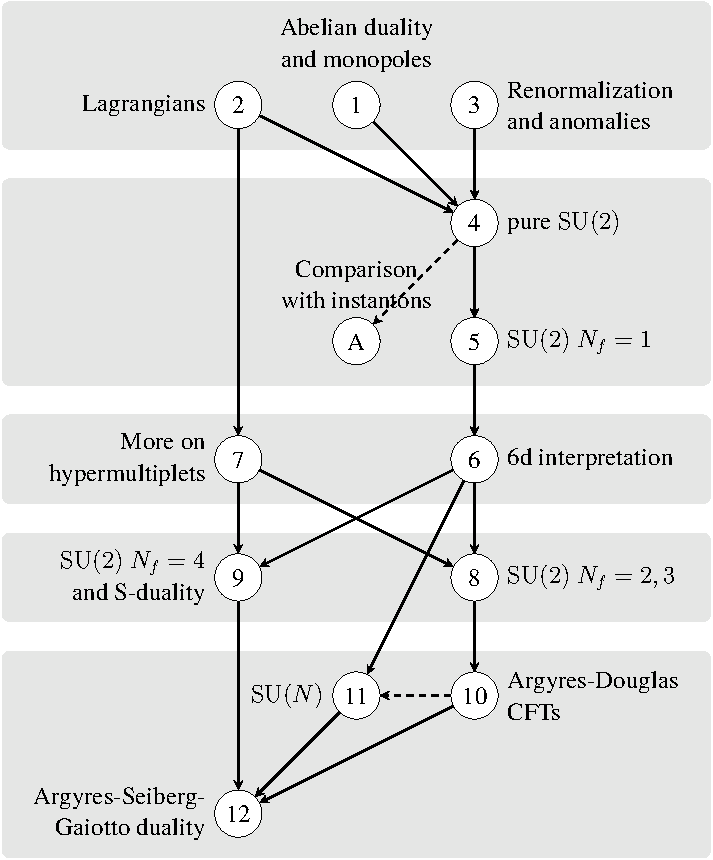
\includegraphics[width=12cm]{relation.pdf}
\caption{本讲义各节之间的依赖关系\label{fig:relation}}
\end{figure}

\section*{预备知识、免责声明与致谢}
\pdfbookmark[1]{预备知识、免责声明与致谢}{prerequisites}
读者需要能够熟练运用 $\cN{=}1$ 超场；我们在第\ref{sec:lagrangian}节约定所用记号。类似地，读者应当了解单圈重整化和微扰反常，并且至少听说过瞬子和单极子，尽管我们会作简短回顾并提供参考文献。本讲义不要求读者预先了解弦论或 M 理论，但读者应当愿意接受定义在维数高于四维的时空上的理论这一概念。除非另有说明，我们沿用物理学中的通常约定：凡是规范代数为 $\mathfrak{su}(N)$ 的规范群，都称为 $\SU(N)$，其他情形亦然。

拉格朗日量各项中的符号和 $i$ 的幂次并非完全一致或正确，但本讲义所呈现的总体思想应当没有问题。作者为使用同一个字母 $i$ 同时表示虚数单位和指标、使用同一个字母 $\theta$ 同时表示 $\theta$ 角和超坐标而致歉。总的来说，作者鼓励读者不仅阅读实际写出的内容，还要读出本来应当写出的内容。想必还存在许多其他排印错误、错误和有待改进之处。作者欢迎你提出任何意见，因此请不要犹豫，欢迎通过电子邮件 \href{mailto:[邮箱隐去]}{\texttt{[邮箱隐去]}} 与作者联系。

引文方面的不足最为明显，因为相关论文的数量极其庞大。作者非常确信，自己引用了过多自己的论文。除此以外，作者至少尝试提供一些近期论文的线索，使感兴趣的读者能够从这些论文的参考文献开始探索相关文献。作者也愿意在本讲义中增补参考文献，再次欢迎任何读者发来邮件。

本讲义根据作者 2011 年在名古屋大学和东北大学，以及 2013 年在立教大学的授课内容整理而成。作者感谢这三所大学的邀请者，使他有机会运用新的技巧综述 $\cN{=}2$ 超对称动力学。他也感谢这些课程的参与者在授课过程中提出的许多有益意见。作者研究这一主题的方法是在与诸多同事的讨论中形成的，并深受这些讨论的影响；本讲义中的大部分新论证，除那些错误的论证之外，都不应归功于作者。Ofer Aharony、Lakshya Bhardwaj、Chi-Ming Chang、Jacques Distler、Sheng-Lan Ko、John Mangual、Satoshi Nawata、Vasily Pestun、Futoshi Yagi 以及一位匿名审稿人，对本讲义初稿提出了有益意见。特别是 Simone Giacomelli、Brian Henning、Greg Moore、Tatsuma Nishioka、Jun'ya Yagi 和 Kazuya Yonekura，详细阅读了初稿，并向作者提出了许多改进建议。能够在此向他们致谢，令作者感到欣慰，也深感荣幸。最后，作者还要感谢 Teppei Kitahara 对插图制作提供的帮助；没有这些插图，本讲义将失去很大一部分价值。

作者还要感谢与其职位相伴的、分量恰到好处的各项职责：这些职责使他不再能够专心从事前沿研究，却仍然有一些时间来总结自己已经知道的内容。尤其要感谢他不得不参加的各种愚蠢的教师会议，本讲义的大部分插图就是在这些会议期间用笔记本电脑绘制的。因此，读者应当感谢东京大学盛行的过度官僚化体制，正是这一体制促成了本讲义的问世。本工作部分得到日本学术振兴会科学研究费补助金第 25870159 号项目资助，部分得到日本文部科学省 WPI 计划对东京大学 IPMU 的资助。

\section{电磁对偶与单极子}\label{sec:emdual}\index{ElectromagneticDuality@电磁对偶|hyperpage}
麦克斯韦理论中交换电场与磁场的电磁对偶，在本讲义中发挥着核心作用。因而，我们不妨先在不引入超对称性这一额外复杂因素的情况下，对它作一回顾。我们也将回顾磁单极子的基本性质。
\subsection{电荷与磁荷}\label{charges}\index{ElectricCharge@电荷|hyperpage}\index{MagneticCharge@磁荷|hyperpage}
考虑一个 $\U(1)$ 规范场，它由规范势 $A=A_\mu dx^\mu$ 和场强 $F=\frac12F_{\mu\nu} dx^\mu \wedge dx^\nu$ 描述，其中 $F_{\mu\nu}=\partial_{[\mu} A_{\nu]}$。场强在规范变换
\begin{equation}
A\to A+i g^{-1} dg
\end{equation}
下不变，其中 $g$ 是从时空到绝对值为一的复数的映射，即 $|g|=1$。我们可以用实函数 $\chi$ 将其写为 $g=e^{i\chi}$，于是得到更熟悉的形式
\begin{equation}
A\to A-d\chi,\label{agauge}
\end{equation}
不过，对我们而言，重要的一点是 $\chi$ 可以是多值的，因此我们作如下等同：
\begin{equation}
\chi\sim \chi+2\pi. \label{chiperiod}
\end{equation}

考虑一个场 $\phi$，其规范变换为
\begin{equation}
\phi \to g^n \phi
\end{equation}
这里，我们要求 $g$ 唯一地确定系统中所有场的变换。因此，$n$ 必须是整数；分数次幂的定义并不唯一。

协变导数为
\begin{equation}
D_\mu\phi = \partial_\mu\phi + inA_\mu \phi,
\end{equation}
而动能项 $|D_\mu\phi|^2$ 是规范不变的。我们将规范场的作用量写为
\begin{equation}
S_\text{Maxwell}=\int d^4 x \frac1{2e^2} F_{\mu\nu} F_{\mu\nu}.\label{maxwell}
\end{equation}
分母中的系数 $2$ 稍显不合惯例，但这一选择会消去后面出现的各种烦人的因子。于是，对场 $\phi$ 量子化得到的两个粒子之间的力，正比于 $e^2n^2$。在唯象学文献中，组合 $en$ 经常被称为电荷，但在本讲义中，我们把整数 $n$ 称为电荷。人们也可能倾向于对 $F$ 作重新标度，以消去上式分母中的因子 $e^2$。不过，我们坚持采用 $\chi$ 的周期为 $2\pi$ 的约定，参见式\eqref{chiperiod}。

在一次量子化框架中，经过 Wick 转动到欧氏号差之后，一个电荷为 $n$ 的带电粒子通过
\begin{equation}
S= in \int_L dx^\mu A_\mu\label{particle}
\end{equation}
与规范场耦合，其中 $L$ 是世界线。在这一描述中，$n$ 的整数性可以如下看出。由于 $\chi$ 具有式\eqref{chiperiod}所示的周期性，线积分 $\int dx^\mu A_\mu$ 只能确定到相差 $2\pi$ 的整数倍。在路径积分中，$e^{iS}$ 必须有良好定义。因而，$n$ 必须是整数。

将式\eqref{maxwell}与式\eqref{particle}相加，并写出 $A_\mu$ 的运动方程，可得
\begin{equation}
\int_{S^2}  \frac{4\pi}{e^2}\vec E \cdot d\vec n=
\int_{S^2}  \frac{4\pi}{e^2} \star F=2\pi n,\label{equantize}
\end{equation}
其中 $E_i=F_{0i}$ 是电场的分量，$S^2$ 是无穷远处的球面，而
\begin{equation}
\star F=\frac12 (\star F)_{\mu\nu} dx^\mu\wedge dx^\nu
\end{equation}
中的
\begin{equation}
(\star F)_{\mu\nu}=\frac12\epsilon_{\mu\nu\rho\sigma} F^{\rho\sigma}
\end{equation}
为对偶场强。我们也会交替使用记号 $\tilde F=\star F$。

接下来，考虑去掉原点的空间。用一个球面包围原点。北、南半球上的规范场 $A_{N,S}$ 在赤道上通过规范变换联系起来：
\begin{equation}
A_N = A_S+ig^{-1} dg
\end{equation}
于是有
\begin{equation}
\int_{S^2} F = \int_{N} F + \int_{S} F = \int_\text{赤道}(A_N-A_S) =\int_{\theta=0}^{\theta =2\pi} \frac{d\chi}{d\theta} d\theta=2\pi m,\label{mquantize}
\end{equation}
其中 $m$ 为整数。我们把 $m$ 称为这一组态的磁荷。库仑型磁场中所含的能量在原点处发散；不过，不必对此过分担心，因为量子化的带电粒子也具有库仑型电场，而该电场的能量同样发散。通过重整化，两者都会变为有限。当 $m$ 非零时，这一组态称为磁单极子。通常，我们简称它为单极子。

\begin{figure}[h]
\[
\inc{angular}
\]
\caption{带电粒子与带磁荷粒子同时存在时产生的角动量。实线箭头、虚线箭头和双线箭头分别表示电场、磁场和坡印廷矢量。\label{fig:angular}}
\end{figure}

在两个分离的点上，分别放置一个电荷为 $n$ 的粒子和一个磁荷为 $m$ 的粒子。两者的电场和磁场共同通过坡印廷矢量，产生绕两点连线方向的角动量，参见图\ref{fig:angular}。仔细计算表明，电磁场中所含的总角动量为 $\hbar nm/2$，这与量子力学中的角动量量子化相一致。

更一般地，我们可以考虑双荷子，即同时具有电荷和磁荷的粒子。如果有一个粒子的电荷为 $n$、磁荷为 $m$，另一个粒子的电荷为 $n'$、磁荷为 $m'$，那么总角动量就是 $\hbar/2$ 乘以
\begin{equation}
 nm'-mn'.
\end{equation}
我们把这一组合称为两组荷 $(n,m)$ 和 $(n',m')$ 的狄拉克配对\index{DiracPairing@狄拉克配对|hyperpage}。

\subsection{S 变换与 T 变换}\label{ST}\index{STransformation@S 变换|hyperpage}\index{TTransformation@T 变换|hyperpage}\index{ComplexifiedCoupling@复化耦合|hyperpage}
麦克斯韦方程为
\begin{equation}
\partial_{[\mu}F_{\nu\rho]}=0,\qquad
\partial_{\mu}F_{\mu\nu}=0
\end{equation}
或等价地，用微分形式记号写为
\begin{equation}
dF=d\star F=0.
\end{equation}
这组方程在交换
\begin{equation}
F\leftrightarrow \star F.
\end{equation}
下不变。用电场 $\vec E$ 和磁场 $\vec B$ 表示，并示意性地记为 $F=(\vec E,\vec B)$，则这一变换的作用为
\begin{equation}
F=(\vec E,\vec B) \longrightarrow
\star F=(\vec B,-\vec E) \longrightarrow
\star^2 F=(-\vec E,-\vec B).
\end{equation}
这一操作经常被称为 $S$ 变换。

为保持式\eqref{equantize}、\eqref{mquantize}中的电荷与磁荷量子化，对偶场强 $F_D$ 和对偶耦合 $e_D$ 必须定义为满足
\begin{equation}
F_D=\frac{4\pi}{e^2}{}\star F,\qquad
\frac{4\pi}{e^2}\frac{4\pi}{e_D^2}=1.
\end{equation}

在这一变换下，荷 $(n,m)$ 按照如下方式变换：
\begin{equation}
\begin{array}{r|ccc}
\text{粒子 1} & (n,m) & \stackrel{S}{\longrightarrow} & (-m,n), \\
\text{粒子 2} &(n',m') & \stackrel{S}{\longrightarrow} & (-m',n'), \\
\text{狄拉克配对} & nm'-n'm & = &  -mn'-(-m')n.
\end{array}
\end{equation}
注意，狄拉克配对在这一操作下保持不变。

假设存在一个中性的实标量场 $\phi$，而 $\U(1)$ 规范场的作用量由下式给出：
\begin{equation}
\frac{1}{2e(\phi)^2} F_{\mu\nu}F_{\mu\nu} + \frac{\theta(\phi)}{16\pi^2} F_{\mu\nu} \tilde F_{\mu\nu}.
\label{u1coupling}
\end{equation}
现在，麦克斯韦方程为
\begin{align}
\partial_{[\mu}F_{\nu\rho]}&=0,\label{MaxwellEq1}\\
\partial_{\mu}\left[ \frac{4\pi}{e(\phi)^2} F_{\mu\nu}+\frac{\theta(\phi)}{2\pi}\tilde F_{\mu\nu}\right]&=0.
\label{MaxwellEq2}
\end{align}
像前面一样作分解 $F=(\vec E,\vec B)$。上述方程表明，满足高斯定律的磁场仍为 $\vec B$，但满足高斯定律的电场现在是如下组合：
\begin{equation}
\vec E_\text{conserved} = \frac{4\pi }{e(\phi)^2} \vec E+\frac{\theta(\phi)}{2\pi} \vec B.
\end{equation}
因此有
\begin{equation}
\int_{S^2} \vec B \cdot d\vec n= 2\pi m,\quad
\int_{S^2} \vec E_\text{conserved} \cdot d\vec n = 2\pi n
\end{equation}
其中 $m$ 和 $n$ 是第\ref{charges}小节引入的整数。这揭示了一个有趣的事实：让我们绝热地改变 $\phi$，从而改变 $\theta(\phi)$。由于 $n$ 是整数，它不能改变。因而，为保持 $\vec E_\text{conserved}$ 不变，$\vec E$ 会获得一个正比于 $\theta(\phi)\vec B$ 的贡献。这称为 Witten 效应\index{WittenEffect@Witten 效应|hyperpage}\cite{Witten:1979ey}。

于是，S 变换交换的是 $(\vec E)_\text{conserved}$ 与 $\vec B$。对偶规范场强 $F_D$ 因此应为
\begin{equation}
F_D=\frac{4\pi}{e(\phi)^2} {}\star F - \frac{\theta}{2\pi}F
\end{equation}
使得式\eqref{MaxwellEq2}恰好成为
\begin{equation}
\partial_{[\mu}F_{D,\nu\rho]}=0.
\end{equation}
我们发现，式\eqref{MaxwellEq1}变为
\begin{equation}
\partial_{\mu}\left[ \frac{4\pi}{e_D(\phi)^2} F_{D,\mu\nu}+\frac{\theta_D(\phi)}{2\pi}\tilde F_{D,\mu\nu}\right]=0
\end{equation}
其中 $e_D(\phi)$、$\theta_D(\phi)$ 由
\begin{equation}
\tau_D(\phi)  = -\frac{1}{\tau(\phi)}
\end{equation}
确定，而
\begin{equation}
\tau(\phi)= \frac{4\pi i}{e(\phi)^2} + \frac{\theta(\phi)}{2\pi},\qquad
\tau_D(\phi)= \frac{4\pi i}{e_D(\phi)^2} + \frac{\theta_D(\phi)}{2\pi}.\label{u1tau}
\end{equation}
这一组合 $\tau(\phi)$ 称为复化耦合。

我们还知道，在量子理论中，$\theta(\phi)$ 与 $\theta(\phi)+2\pi$ 无法区分，因为欧氏路径积分中的被积函数仅改变一个因子
\begin{equation}
\exp\left[i\int d^4x \frac{1}{8\pi}  F_{\mu\nu} \tilde F_{\mu\nu}\right]
\end{equation}
而该因子始终为一\footnote{严格地说，这仅在自旋流形上成立。注意，$\int d^4x (8\pi)^{-1}  F_{\mu\nu} \tilde F_{\mu\nu}= \pi \int (F/2\pi)^2=\pi \int c_1(F)^2$。在自旋流形上，交叉形式为偶形式，最后一个表达式是 $2\pi$ 的整数倍。有关非自旋流形上的细微问题，参见文献\cite{Witten:1995gf}。}。我们将其称为 $T$ 变换。不过，它确实会通过加上 $\vec B$ 而改变 $\vec E_\text{conserved}$。等价地，它使荷 $(n,m)$ 发生如下变化：
\begin{equation}
\begin{array}{r|ccc}
\text{粒子 1} & (n,m) & \stackrel{T}{\longrightarrow} & (n+m,m), \\
\text{粒子 2} &(n',m') & \stackrel{T}{\longrightarrow} & (n'+m',m'), \\
\text{狄拉克配对} & nm'-n'm & = &  (n+m)m'-(n'+m')m.
\end{array}
\end{equation}
可以看到，两个粒子的狄拉克配对保持不变。它对复化耦合 $\tau(\phi)$ 的作用为
\begin{equation}
\tau(\phi)_\text{old}  \stackrel{T}{\longrightarrow} \tau(\phi)_\text{new} = \tau(\phi)_\text{old}+1.
\end{equation}
变换 $S$ 与 $T$ 生成 $\SL(2,\bZ)$ 对荷 $(n,m)$ 的作用：
\begin{align}
S&=\begin{pmatrix}
0&-1\\1&0
\end{pmatrix}, &
S \begin{pmatrix}n \\ &=
\begin{pmatrix}-m \\,&
S\tau &= -\frac1\tau \label{S}\\
T&=\begin{pmatrix}1&1\\0&1\end{pmatrix}, &
T \begin{pmatrix}n \\ &=
\begin{pmatrix}n+m \\,&
T\tau &= \tau+1. \label{T}
\end{align}
一般而言，它对 $\tau$ 的作用为分式线性变换
\begin{equation}
\begin{pmatrix}a&b \\c&d\end{pmatrix} \in \SL(2,\bZ) :
\tau \to \frac{d\tau+b}{c\tau+a}.
\end{equation}

\subsection{'t Hooft-Polyakov 单极子}\label{sec:monopole}\index{HooftPolyakovMonopole@'t Hooft-Polyakov 单极子|hyperpage}
这里，我们总结磁单极子的一些性质，后面将反复引用这些性质。有关本小节所讨论内容的详细阐述，读者可参阅文献\cite{Harvey:1996ur,Weinberg:2006rq}等综述，或教科书\cite{Shifman}。Coleman 的综述\cite{Coleman:1982cx}也非常具有启发性。\footnote{遗憾的是，这篇综述并未收入《Aspects of Symmetry》一书。R.~Stora 所译的法文版本也可见于文献\cite{Coleman1982cxF}，其排版比文献\cite{Coleman:1982cx}中的版本精美得多。}
\subsubsection{经典性质}\index{BPSBound@BPS 界|hyperpage}\index{BPSEquation@BPS 方程|hyperpage}
考虑一个含有伴随表示标量场的 $\SU(2)$ 规范理论，其作用量为
\begin{equation}
S=\int d^4 x\frac{1}{g^2}\left[\frac{1}{2}\tr F_{\mu\nu} F_{\mu\nu} + \tr D_\mu\Phi D_\mu\Phi \right].
\end{equation}
场 $\Phi$ 是一个无迹厄米 $2\times 2$ 矩阵。

考虑满足
\begin{equation}
\Phi= \begin{pmatrix}a & 0 \\0 & -a\end{pmatrix}.\label{phivev}
\end{equation}
的真空。当 $a\neq 0$ 时，$\SU(2)$ 规范对称性破缺为 $\U(1)$。事实上，真空期望值\eqref{phivev}与具有如下形式的规范场强对易：
\begin{equation}
F_{\mu\nu}=\begin{pmatrix}
F_{\mu\nu}^{\U(1)} & 0\\
0 & -F_{\mu\nu}^{\U(1)}
\end{pmatrix}\label{u1embed}
\end{equation}
其中 $F_{\mu\nu}^{\U(1)}$ 是按照第\ref{charges}小节约定归一化的 $\U(1)$ 规范场强。注意，标量场 $\Phi$ 的非对角分量的量子，相对于这一 $\U(1)$ 场具有电荷 $\pm 2$；这可以通过展开协变导数得出。

我们考虑的是规范理论，因此场 $\Phi$ 不必严格取为式\eqref{phivev}右端的形式。相反，我们只需要 $\Phi$ 的本征值为 $\pm a$。因而，可以考虑如下形式的组态：
\begin{equation}
\Phi(x)=\frac{x_i \sigma^i}{|x|} f(|x|) a
\label{tHP}
\end{equation}
其中 $i=1,2,3$，而 $f(r)$ 是满足
\begin{equation}
\lim_{r\to 0} f(r)=0,\qquad
\lim_{r\to \infty} f(r)=1.
\end{equation}
的无量纲函数。在空间无穷远处，$\Phi$ 的真空期望值与式\eqref{phivev}共轭，因此这一组态可被视为式\eqref{phivev}所给真空的激发。

$\SU(2)$ 中未破缺的 $\U(1)$ 沿着 $\Phi$ 的方向。因而，至少在 $r\gg 0$ 时，$\U(1)$ 场强 $F_{\mu\nu}^{\U(1)}$ 的一个更一般的定义是如下组合：
\begin{equation}
F_{\mu\nu}^{\U(1)}:=\frac{1}{2a}\tr F_{\mu\nu} \Phi .\label{gauge-inv-def-of-u1}
\end{equation}
在 $r\gg 0$ 的区域中，尝试通过一个规范变换将组态\eqref{tHP}化为式\eqref{phivev}。除南极点以外，这可以光滑地实现，所用的规范变换为
\begin{equation}
\exp[ i\frac{\varphi}{2} (-\sigma^1 \sin\theta + \sigma^2 \cos\theta )],\quad
\text{其中}\quad \frac{\vec x}{|x|}=(\cos\varphi,\sin\varphi\cos\theta,\sin\varphi\sin\theta).
\end{equation}
由此得到的南极点附近的规范变换为
\begin{equation}
i (-\sigma^1 \sin\theta + \sigma^2\cos\theta) =  \exp[ -i\theta \sigma^3 ] \cdot (i\sigma^2).
\end{equation}
当 $\theta$ 从 $0$ 变到 $2\pi$ 时，可以看到 $\U(1)$ 场 $F^{\U(1)}_{\mu\nu}$ 的磁荷为 $m=1$，因此它是一个单极子。这一结果最初由 't Hooft 和 Polyakov 发现。注意，它与场 $\Phi$ 的粒子的狄拉克配对为 2，是最小允许值的两倍。

我们来计算这一场组态中所含的能量。动能为 $1/g^2$ 乘以下式：
\begin{align}
\int d^3x \left[\tr B_{i} B_i + \tr D_i\Phi D_i\Phi \right]
&=\int d^3 x \left[ \tr(B_i\mp D_i\Phi)^2 \pm 2 \tr B_i D_i\Phi \right]\\
&\ge \pm 2 \int d^3 x  \tr B_i D_i\Phi = \pm 2 \int d^3 x \partial_i \tr B_i\Phi \\
&= \pm 2 \int_{S^2}  d\vec n \cdot \tr \vec B\Phi
\end{align}
其中最后一个积分是在空间无穷远处的球面上进行的。根据式\eqref{gauge-inv-def-of-u1}，它等于 $\pm 2(2a)(2\pi m)$，其中 $m$ 为磁荷。因而得到下界
\begin{equation}
\text{（单极子的能量）}\ge \frac{4\pi }{g^2} (2a) |m|  \label{monopole-energy}
\end{equation}
这称为 Bogomolnyi-Prasad-Sommerfield（BPS）界。当且仅当
\begin{equation}
B_i=\pm D_i\Phi,
\end{equation}
时，该不等式取等号；这一方程称为 BPS 方程。它确定了式\eqref{tHP}中函数 $f(r)$ 的形式。

\subsubsection{半经典性质}\index{ZeroModes@零模|hyperpage}\index{Dyon@双荷子|hyperpage}\index{SemiclassicalQuantization@半经典量子化|hyperpage}\index{FlavorSpinor@味旋量|hyperpage}
给定这样一个显式的单极子解，我们可以利用对称性构造与它相关的其他解。首先，组态\eqref{tHP}的中心位于坐标系原点。可以把单极子的中心平移到空间 $\bR^3$ 中的任意一点 $\vec y$。由此得到三个零模。

另一个零模由如下规范变换得到：
\begin{equation}
e^{ i \alpha \Phi/a }\label{gauge-zm}
\end{equation}
注意，在无穷远处为零的规范变换是物理系统的一种冗余，而在无穷远处不为零的规范变换则被认为会改变经典组态。对一般的 $\alpha$，变换\eqref{gauge-zm}会改变 $F_{ij}(x)$ 的渐近行为；但在 $\alpha=\pi$ 时，这一变换对伴随表示中的场作用平凡。因此，$\alpha$ 是一个取值范围为 $0\le\alpha<\pi$ 的角变量。

单极子的半经典量子化涉及非零模的 Fock 空间，以及依赖于零模 $\vec y$ 和 $\alpha$ 的波函数 $\psi(\vec y,\alpha)$。沿 $\vec y$ 方向的波函数描述单极子质心的空间运动。沿 $\alpha$ 方向的波函数则描述单极子的电荷，这一点可以如下看出。

将式\eqref{gauge-zm}与式\eqref{u1embed}、\eqref{gauge-inv-def-of-u1}比较，可以看到，未破缺的 $\U(1)$ 整体规范变换 $e^{i\varphi}$ 使 $\alpha$ 平移为
\begin{equation}
\alpha\to \alpha+\varphi.\label{shift-el}
\end{equation}
回顾一下，电荷为 $n$ 的态 $\ket\psi$ 在 $\U(1)$ 整体变换 $e^{i\varphi}$ 下按照
\begin{equation}
\ket\psi \to e^{in\varphi} \ket\psi.\label{www}
\end{equation}
变换。现在，由于 $\alpha$ 是周期为 $\pi$ 的变量，$\psi(\alpha)$ 可以展开为 $e^{i2d\alpha}$ 的线性组合，其中 $d$ 为整数。在变换\eqref{shift-el}下，波函数按照式\eqref{www}中 $n=2d$ 的情形变换，因此，具有这一零模波函数的单极子态的电荷为 $2d$。

总之，由半经典量子化得到的电荷与磁荷组合 $(n,m)$ 具有 $(n,m)=(2d,1)$ 的形式，其中 $d$ 为整数。这一结果最初由 Julia 和 Zee 发现：一旦对 't Hooft-Polyakov 单极子进行量子化，我们得到的就不仅是一个纯磁单极子，而是从 $d=-\infty$ 到 $+\infty$ 的一整塔双荷子态。

最后，考虑 't Hooft-Polyakov 单极子\eqref{tHP}中的费米子零模的效应。首先考虑伴随表示中的两个 Weyl 费米子 $\lambda$、$\tilde\lambda$，其拉格朗日量为
\begin{equation}
\tr \bar\lambda \slash D \lambda + \tr\bar{\tilde\lambda} \slash D \tilde\lambda
+ c(\tr  \lambda [\Phi,  \tilde\lambda ] + \tr \bar \lambda [\Phi,\bar{\tilde\lambda}]).
\end{equation}
将协变导数 $D$ 中的规范势以及标量场都视为背景，并把 $\lambda$、$\tilde\lambda$ 分解成角动量本征态。轨道角动量的下界由狄拉克配对给出，在这里等于 $\hbar$。旋量场的自旋为 $\hbar/2$。因此，最低角动量的态具有 $\hbar/2$ 的自旋。已知当系数 $c$ 取值于某一区间时，存在一对零模 $b_\alpha$，其中 $\alpha=1,2$ 是空间转动群 $\SO(3)$ 的旋量指标。半经典量子化将它们提升为一对费米子振子：
\begin{equation}
\{b_\alpha,b_\beta^\dagger\}=\delta_{\alpha\beta}.
\end{equation}
从玻色部分半经典量子化得到的一个态 $\ket\psi$ 出发，它们产生四个态：
\begin{equation}
\begin{array}{ccccc}
&\raisebox{-.8ex}{\rotatebox{30}{$\leftrightarrow$}}& b^\dagger_1 \ket\psi & \leftrightarrow & b^\dagger_1 b^\dagger_2 \ket\psi \\
\ket\psi & \leftrightarrow & b^\dagger_2\ket\psi & \rotatebox{30}{$\leftrightarrow$}
\end{array}.
\end{equation}
这相当于一个复玻色子和一个费米子。

假设再引入一对伴随 Weyl 费米子 $\lambda'$、$\tilde\lambda'$。那么将得到另一对费米子振子 $b_\alpha'$。它们共同生成 $2^4=16$ 个态，包括一个有质量矢量（有 3 个态）、四个有质量旋量（有 8 个态）以及五个有质量标量。

接下来，考虑二重态表示中的 $2N$ 个 Weyl 费米子 $\psi_i^a$，其中 $a=1,2$，$i=1,\ldots,2N$，其拉格朗日量为
\begin{equation}
 \bar\psi_i \slash D \psi_i
+ c'  (\psi^a_i \Phi_{(ab)}  \psi^b_i +\bar\psi^a_i \Phi_{(ab)}  \bar\psi^b_i ).
\end{equation}
注意，该拉格朗日量具有作用于指标 $i$ 的 $\SO(2N)$ 味对称性。

现在，$\psi$、$\tilde\psi$ 的量子相对于未破缺的 $\U(1)$ 的电荷为 $1$。因而，狄拉克配对为 $\hbar/2$。与内禀自旋 $\hbar/2$ 作张量积，可知最小轨道角动量为 $0$。已知适当选择 $c'$ 后，该费米子系统具有零模 $\gamma_i$，$i=1,\ldots,2N$。半经典量子化之后，它们成为一组满足如下对易关系的费米子算符：
\begin{equation}
\{\gamma_i,\gamma_j\}=\delta_{ij}.
\end{equation}
这就是 $\SO(2N)$ 的伽马矩阵的对易关系。单极子态构成 $\gamma_i$ 的表示，这意味着它们按照味对称群 $\SO(2N)$ 的旋量表示变换。

$\SU(2)$ 规范对称性二重态表示中的场还有另一个效应。即在规范零模\eqref{gauge-zm}中，$\alpha=\pi$ 给出矩阵
\begin{equation}
\begin{pmatrix}-1 & 0 \\0 & -1\end{pmatrix}
\end{equation}
它对二重态表示中的场具有非平凡作用。于是，规范零模 $\alpha$ 的周期现在是 $2\pi$，沿 $\alpha$ 方向的波函数可以取为任意整数 $n$ 对应的 $e^{in\alpha}$。因此，电荷 $n$ 既可以为偶数，也可以为奇数。算符 $\gamma_i$ 来自二重态表示中场的模，因此会使电荷改变 $\pm1$。

可以通过
\begin{equation}
\Gamma=\gamma_1\gamma_2 \cdots \gamma_{2N},
\end{equation}
定义味旋量的手征性 $\Gamma$，从而将 $\SO(2N)$ 的旋量分解为正手征和负手征旋量。算符 $\gamma_i$ 的作用会改变味旋量的手征性。结合上一段所见的 $\U(1)$ 电荷的行为，我们得出结论：单极子态的 $\U(1)$ 电荷的奇偶性，与味旋量表示的手征性相关。

\section{$\cN{=}2$ 多重态与拉格朗日量}\label{sec:lagrangian}

\subsection{微观拉格朗日量}
\subsubsection{$\cN{=}1$ 超场}\index{Superfield@超场|hyperpage}\index{ChiralMultiplet@手征多重态|hyperpage}\index{AuxiliaryField@辅助场|hyperpage}
现在转向具有 $\cN{=}2$ 超对称性的拉格朗日量的构造。一个 $\cN{=}2$ 超对称理论，特别地也是一个 $\cN{=}1$ 超对称理论。因而，用 $\cN{=}1$ 超场来描述 $\cN{=}2$ 系统很方便。为此，先简要回顾 $\cN{=}1$ 形式体系。仅在本节中，我们将虚数单位写成 $\ii$，以示区别。

一个 $\cN{=}1$ 矢量多重态由一个 Weyl 费米子 $\lambda_\alpha$ 和一个矢量场 $A_\mu$ 组成，二者都属于规范群 $G$ 的伴随表示。将它们合并为超场 $W_\alpha$，其展开为
\begin{equation}
W_\alpha=\lambda_\alpha+F_{(\alpha\beta)}\theta^\beta + D\theta_\alpha+\cdots
\end{equation}
其中 $D$ 是辅助场，同样属于规范群的伴随表示。$F_{\alpha\beta}=\frac \ii2 \sigma^\mu{}^\beta_{\dot\gamma} \bar\sigma^{\nu}{}^{\dot \gamma}_\alpha F_{\mu\nu}$ 是场强 $F_{\mu\nu}$ 的反自对偶部分。

矢量多重态的动能项为
\begin{equation}
\int d^2\theta \frac{-\ii}{8\pi} \tau \tr W_\alpha W^\alpha + cc.
\end{equation}
其中
\begin{equation}
\tau=\frac{4\pi \ii}{g^2}+\frac{\theta}{2\pi}
\end{equation}
是将耦合常数的倒数与 $\theta$ 角合并而成的复数。我们将其称为规范多重态的复化耦合。按分量展开，得到
\begin{equation}
\frac{1}{2g^2} \tr F_{\mu\nu}F^{\mu\nu} + \frac{\theta}{16\pi^2} \tr F_{\mu\nu} \tilde F^{\mu\nu} + \frac{1}{g^2}\tr D^2 -\frac{2\ii}{g^2}\tr \bar\lambda\slash\partial \lambda.
\end{equation}
对于规范代数的标准生成元，我们采用约定 $\tr T^a T^b = \frac12 \delta^{ab}$，这就解释了规范动能项前为何出现因子 $1/(2g^2)$。$\theta$ 项是一个规范依赖项的全导数，因此不影响微扰计算。它确实会影响非微扰计算，我们将在后面回到这一点。

一个 $\cN{=}1$ 手征多重态 $Q$ 由一个复标量 $Q$ 和一个 Weyl 费米子 $\psi_\alpha$ 组成，二者属于规范群的同一表示。用超场表示，有
\begin{equation}
Q=Q\big|_{\theta=0} + 2\psi_\alpha \theta^\alpha + F \theta_\alpha \theta^\alpha
\end{equation}
其中 $F$ 为辅助场。中间分量前的系数 2 不合通常惯例，但这一选择使我们能够消去后面公式中出现的各种烦人的 $\sqrt{2}$ 因子。手征多重态 $Q_{1,\ldots}$ 可以属于规范群 $G$ 的任意复表示 $R$。此时，拉格朗日密度为
\begin{equation}
\int d^4\theta Q^\dagger{}^{j} e^{V^a \rho_a{}^{i}_{j}} Q_i + \int d^2\theta W(Q)+ cc.
\end{equation}
其中 $V$ 是矢量超场，$\rho_a{}^i_j$ 是规范代数的矩阵表示，而 $W(Q)$ 是 $Q_{1,\ldots}$ 的规范不变全纯函数。

要求各个场的超对称变换为零，即可得到超对称真空。非平凡条件来自
\begin{equation}
\delta \lambda_\alpha =0, \qquad \delta\psi_\alpha=0
\end{equation}
它们给出
\begin{equation}
D_a=0, \quad F_i=0.
\end{equation}
解出辅助场的代数运动方程，得到
\begin{equation}
Q^\dagger_{\bar j} \rho_a^{\bar ji}Q_i =0,\quad
\frac{\partial W}{\partial Q_i}=0.
\end{equation}

\subsubsection{矢量多重态与超多重态}\label{sec:hyperdef}\index{VectorMultiplet@矢量多重态|hyperpage}\index{Hypermultiplet@超多重态|hyperpage}\index{RSymmetry@R 对称性|hyperpage}\index{HalfHypermultiplet@半超多重态|hyperpage}\index{NFourTheory@$\cN{=}4$ 理论|hyperpage}\index{NTwoStarTheory@$\cN{=}2^*$ 理论|hyperpage}
一个 $\cN{=}2$ 矢量多重态由如下两个 $\cN{=}1$ 多重态组成，二者都属于规范群 $G$ 的伴随表示：
\begin{equation}
\begin{array}{ccccc@{\qquad}c}
&\raisebox{-.8ex}{\rotatebox{30}{$\leftrightarrow$}}& \lambda_\alpha & \leftrightarrow & A_\mu & \text{$\cN{=}1$ 矢量多重态},\\
\Phi & \leftrightarrow & \tilde\lambda _\alpha &  \rotatebox{30}{$\leftrightarrow$} &  & \text{$\cN{=}1$ 手征多重态}.
\end{array}
\end{equation}
这里，水平箭头表示在 $\cN{=}1$ 超场形式体系中显式呈现的 $\cN{=}1$ 子超对称生成元，斜箭头则对应第二组 $\cN{=}1$ 子超对称性。

构造第二组超对称作用的一种简单方法，是要求理论在作用于 $\lambda_\alpha$ 和 $\tilde\lambda_\alpha$ 的 $\SU(2)$ 转动下对称。一般而言，不与超对称生成元对易的对称性称为 R 对称性。因而，这一 $\SU(2)$ 对称性经常被称为 $\SU(2)_R$ 对称性。将超场形式体系中显式的超对称性与某个 R 对称性结合起来，构造具有更多超对称性的理论，如今已经是一种标准技巧；有关应用，可参见文献\cite{Aharony:2008ug}。还应当记住，不具有 $\SU(2)_R$ 对称性的 $\cN{=}2$ 超对称理论是可能存在的，而且确实存在：可以只有两组超对称生成元，而没有联系它们的 $\SU(2)$ 对称性，例如参见文献\cite{Antoniadis:1995vb,FujiwaraItoyamaSakaguchi}。尽管如此，为简单起见，本讲义只讨论具有 $\SU(2)_R$ 对称性的 $\cN{=}2$ 超对称系统。

此时拉格朗日量为
\begin{equation}
\frac{\Im\tau}{4\pi} \int d^4\theta \tr \Phi^\dagger e^{[V,\cdot]} \Phi +\int d^2\theta \frac{-\ii}{8\pi}\tau \tr W_\alpha W^\alpha + cc.\label{vectorlag}
\end{equation}
凯勒势与规范动能项前的系数之比，由 $\SU(2)_R$ 对称性的要求确定。

一个 $\cN{=}2$ 超多重态\footnote{有一个愚蠢的惯例：拼写“vector multiplets”时，要在“vector”和“multiplets”之间加空格，而拼写“hypermultiplets”时却不加空格。在口语中，hypermultiplets 经常简称为 hypers。}包含如下各场：
\begin{equation}
\begin{array}{ccccc@{\qquad}c}
&\raisebox{-.8ex}{\rotatebox{30}{$\leftrightarrow$}}& Q & \leftrightarrow & \psi & \text{$\cN{=}1$ 手征多重态}\\
\tilde\psi^\dagger & \leftrightarrow &\tilde Q^\dagger &   \rotatebox{30}{$\leftrightarrow$}  &  & \text{$\cN{=}1$ 反手征多重态}
\end{array}
\end{equation}
它们都属于规范群的同一表示 $R$。因而，$\cN{=}1$ 手征多重态 $Q$ 和 $\tilde Q$ 属于规范群的共轭表示。为使理论具有 $\cN{=}2$ 超对称性，我们再次要求它在作用于 $Q$ 和 $\tilde Q^\dagger$ 的 $\SU(2)$ 转动下对称。

为具体起见，考虑 $G=\SU(N)$ 以及基本 $N$ 维表示中的 $N_f$ 个超多重态 $Q_i^a$、$\tilde Q^i_a$，其中 $a=1,\ldots,N$，$i=1,\ldots,N_f$。这组场经常被称为 $\SU(N)$ 的 $N_f$ 个基本表示味。规范变换对它们的作用为
\begin{equation}
Q_i \to e^{\Lambda} Q_i,\qquad
\tilde Q^i \to  \tilde Q^i e^{-\Lambda}
\end{equation}
其中 $\Lambda$ 是由手征超场组成的无迹 $N\times N$ 矩阵；这里省略了规范指标。

超多重态的拉格朗日量为
\begin{equation}
c\int d^4\theta (Q^\dagger{}^i e^V Q_i+ \tilde Q^i e^{-V} \tilde Q^\dagger{}_i)
+c'(\int d^2 \theta \tilde Q^i \Phi Q_i + cc.)
+(\int d^2\theta \mu^i_j \tilde Q^jQ_i + cc.)\label{hyperlag}
\end{equation}
其中再次省略了规范指标 $a$。$\SU(2)_R$ 对称性的存在确定了 $c$ 与 $c'$ 的比值：例如，可以比较第一项中 $Q^i\lambda\psi$ 的系数和第二项中 $\tilde Q^i\tilde\lambda\psi$ 的系数。我们发现，取 $c=c'$ 即可。除非另有说明，以下均取 $c=c'=1$。$\SU(2)_R$ 对称性还要求质量项 $\mu^i_j$ 满足 $[\mu,\mu^\dagger]=0$。因此，$\mu$ 可以对角化，质量项也就经常写为
\begin{equation}
\sum_i \int d^2\theta \mu_i \tilde Q^i Q_i + cc.
\end{equation}

作为另一个例子，考虑伴随表示中的一个超多重态 $(Z,\tilde Z)$，即二者都是 $N\times N$ 无迹矩阵。以下讨论也很容易推广到任意规范群。当超多重态无质量时，总拉格朗日量具有如下形式：
\begin{multline}
\int d^2\theta \frac{-\ii}{8\pi}\tau \tr W_\alpha W^\alpha + cc.
+\frac{\Im\tau}{4\pi} \int d^4\theta \tr \Phi^\dagger e^{[V,\cdot]} \Phi \\
+\frac{\Im\tau}{4\pi} \int d^4\theta (Z^\dagger{} e^{[V,\cdot]} Z+ \tilde Z e^{-[V,\cdot]} \tilde Z^\dagger{})
+\frac{\Im\tau}{4\pi} \int d^2 \theta \tilde Z [\Phi, Z] + cc.\label{n4lag}
\end{multline}
这里，我们对式\eqref{hyperlag}中的 $c=c'$ 作了不同选择。这一拉格朗日量显然具有转动 $\Phi$、$Z$ 和 $\tilde Z$ 的 $\SU(3)_F$ 味对称性。它与超场形式体系中显式的 $\cN{=}1$ 超对称性对易。我们还知道，该理论具有转动 $Z$ 和 $\tilde Z^\dagger$ 的 $\SU(2)_R$ 对称性。$\SU(3)_F$ 与 $\SU(2)_R$ 这两个对称性不对易：我们发现，存在作用于
\begin{equation}
\Re \Phi, \Im \Phi, \Re Z, \Im Z, \Re \tilde Z, \Im \tilde Z.
\end{equation}
的 $\SO(6)_R$ 对称性。注意，$\SO(6)_R$ 也可以视为 $\SU(4)_R$，因为 $\SO(6)$ 与 $\SU(4)$ 具有相同的李代数。于是，$\SU(4)_R$ 对称性作用于系统中的四个 Weyl 费米子
\begin{equation}
\lambda, \tilde\lambda, \psi, \tilde \psi
\end{equation}
其中 $\lambda$ 和 $\tilde\lambda$ 属于 $\cN{=}2$ 矢量多重态，而 $\psi$、$\tilde\psi$ 属于 $\cN{=}2$ 超多重态。我们得出结论，该系统实际上具有 $\cN{=}4$ 超对称性，其四个超对称生成元受 $\SU(4)_R\simeq\SO(6)_R$ 作用。这里的论证，是结合超场形式体系中显式与非显式对称性的又一次应用。

可以向式\eqref{n4lag}加入质量项 $\int d^2\theta \mu Z\tilde Z + cc.$。它保持 $\cN{=}2$ 超对称性，但破坏 $\cN{=}4$ 超对称性。得到的理论有时称为 $\cN{=}2^*$ 理论。

在结束这一小节之前，还应当提及半超多重态的概念。从一个完整超多重态 $(Q_a,\tilde Q^a)$ 出发，其中 $Q_a$ 与 $\tilde Q^a$ 分别属于表示 $R$ 和 $\bar R$。当 $R$ 为赝实表示，或等价地，当存在反对称不变张量 $\epsilon_{ab}$ 时，可以施加与 $\cN{=}2$ 超对称性相容的约束
\begin{equation}
Q_a=\epsilon_{ab} \tilde Q^b
\end{equation}
使多重态中的自由度数目减半。所得多重态称为表示 $R$ 中的半超多重态。第\ref{sec:hyperrevisited}小节还将回到这一概念。

\subsection{真空}\label{sec:classicalvac}\index{SupersymmetricVacuum@超对称真空|hyperpage}\index{CoulombBranch@库仑支|hyperpage}\index{HiggsBranch@希格斯支|hyperpage}\index{MixedBranch@混合支|hyperpage}\index{DTerm@D 项|hyperpage}\index{FTerm@F 项|hyperpage}

矢量多重态与超多重态组成的系统，其拉格朗日量是式\eqref{vectorlag}与式\eqref{hyperlag}之和。超对称真空由以下条件给出。

首先，对辅助场 $D$ 变分得到
\begin{equation}
\frac{1}{g^2}[\Phi^\dagger,\Phi]+ (Q_i Q^\dagger{}^i-\tilde Q^\dagger{}_i \tilde Q^i)\big|_\text{traceless}=0,\label{Deq}
\end{equation}
其中，对于一个 $N\times N$ 矩阵，$X|_\text{traceless}$ 定义为
\begin{equation}
X|_\text{traceless}=X-\frac1N\tr X.
\end{equation}
我们约定，在需要时将标量乘以单位矩阵。

其次，对 $\Phi$ 的辅助场 $F$ 变分得到
\begin{equation}
Q_i \tilde Q^i \big|_\text{traceless}=0\label{Feq}
\end{equation}
而 $Q_i$、$\tilde Q^i$ 的辅助场 $F$ 给出
\begin{equation}
\Phi Q_i +\mu^j_i Q_j =0, \qquad \tilde Q^i \Phi + \mu^i_j \tilde Q^j=0 \label{Qeq}
\end{equation}
它们对所有 $i$ 都成立。总标量势是式\eqref{Deq}、\eqref{Feq}和\eqref{Qeq}中各表达式的绝对值平方的加权和。

到目前为止，我们只使用了相对于超场记号中显式的 $\cN{=}1$ 超对称性的超对称条件。对式\eqref{Deq}第一项与第二项之间的交叉项作适当整理，再与式\eqref{Qeq}的平方项合并，就可以把总标量势重写为下列各对象的加权和。首先，有一个只含 $\Phi$ 的项：
\begin{equation}
[\Phi^\dagger,\Phi]=0.\label{phieq}
\end{equation}
其次，有只含 $Q$ 和 $\tilde Q$ 的项，其中之一为
\begin{equation}
(Q_i Q^\dagger{}^i-\tilde Q^\dagger{}_i \tilde Q^i)\big|_\text{traceless}=0\label{tripleteq}
\end{equation}
另一个则是式\eqref{Feq}。最后，还有混合 $\Phi$ 和 $Q$ 的项，即式\eqref{Qeq}以及
\begin{equation}
\Phi^\dagger Q_i +\mu^\dagger{}^j_i Q_j =0, \qquad \tilde Q^i \Phi^\dagger + \mu^\dagger{}^i_j \tilde Q^j=0 \label{QQeq}.
\end{equation}

注意，式\eqref{phieq}与式\eqref{tripleteq}分别是方程\eqref{Deq}的 $\SU(2)_R$ 单态部分和三重态部分。此外，方程\eqref{tripleteq}与方程\eqref{Feq}的实部和虚部共同构成 $\SU(2)_R$ 的三重态。最后，方程\eqref{Qeq}与方程\eqref{QQeq}按照 $\SU(2)_R$ 的二重态变换。

总结一下。我们最初在式\eqref{Deq}、\eqref{Feq}和\eqref{Qeq}中要求一组 $\cN{=}1$ 子超对称性不破缺。随后发现，所满足的方程自动具有 $\SU(2)_R$ 不变性，因此全部 $\cN{=}2$ 超对称性也就自动保持不破缺。

获得超对称性的一种简单方式，是要求式\eqref{phieq}成立并令 $Q=\tilde Q=0$。超对称真空模空间的这一子空间称为库仑支，因为通常在红外仍有若干阿贝尔规范场保留下来。

当质量项 $\mu^i_j$ 非零时，一般而言，其他真空组态的讨论并不直接。当 $\mu^i_j=0$ 时，还存在另一类真空组态，只需要求式\eqref{tripleteq}与式\eqref{Feq}成立，并令 $\Phi=0$。这称为希格斯支。这一领域中的一些人只把规范群完全破缺的分支称为希格斯支；但从理论上说，这里所定义的希格斯支在各种操作下具有更统一的行为。

超多重态中的标量 $Q$、$\tilde Q$ 与矢量多重态中的标量 $\Phi$ 同时非零的分支，称为混合支。

由式\eqref{phieq}可知，在超对称真空中，$\Phi$ 可以对角化。为具体起见，令 $G=\SU(2)$。此时 $\Phi=\diag(a,-a)$。当 $a\neq0$ 时，规范群破缺为 $\U(1)$。由于红外仍有库仑场存在，这些真空称为库仑支。下面计算由此产生的 W 玻色子的质量。由
\begin{equation}
\frac1{g^2}\tr|D_\mu \Phi|^2 = \frac1{g^2}\tr (\partial_\mu \Phi+[A_\mu,\Phi])^2
\end{equation}
可知，拉格朗日量中存在一项
\begin{equation}
\frac1{g^2}\tr [A_\mu,\vev{\Phi}]^2
\end{equation}
它赋予矢量场以质量。写成
\begin{equation}
A_\mu=\begin{pmatrix}A^0 & W^+ \\W^- & -A^0\end{pmatrix}_\mu,
\end{equation}
可得
\begin{equation}
\left[
\begin{pmatrix}0 & W^+_\mu \\0 & 0\end{pmatrix},
\begin{pmatrix}a & 0\\0 & -a\end{pmatrix}
\right]=-2a \begin{pmatrix}0 & W^+_\mu \\0 & 0\end{pmatrix}.
\end{equation}
在我们的约定中，动能项为 $\tr F_{\mu\nu}F_{\mu\nu}/(2g^2)$，因此得到质量
\begin{equation}
M_W=|2a|.
\end{equation}
对于固定的 $i$，场 $Q_i$、$\tilde Q^i$ 的质量项为
\begin{equation}
\tilde Q^i \Phi Q_i+ \mu_i \tilde Q^i Q_i =
(\tilde Q_1^i, \tilde Q_2^i)
\begin{pmatrix}a+\mu_i & 0 \\0 & -a+\mu_i\end{pmatrix}
\begin{pmatrix}Q_1^i \\Q_2^i\end{pmatrix}.
\end{equation}
因此有
\begin{equation}
M_{Q_{i,1}}=|a+\mu|,\qquad
M_{Q_{i,2}}=|{-a}+\mu|.
\end{equation}

在 $\theta=0$ 的情形下，我们已经在式\eqref{monopole-energy}中研究了这一模型的单极子的经典质量。一般而言，它由
\begin{equation}
M_\text{monopole}=|2\tau a|.
\end{equation}
给出。经典地，粒子的质量满足一个一般不等式：
\begin{equation}
M \geq |na+m(2\tau a) + \sum_i f_i \mu_i| \label{classicalBPS}
\end{equation}
其中 $n$、$m$、$f_i$ 分别为粒子的电荷、磁荷和味荷。这里，第 $i$ 个味荷对应于对称性
\begin{equation}
Q_i \to e^{\ii\varphi_i} Q_i,\quad
\tilde Q^i \to e^{-\ii\varphi_i} \tilde Q^i.
\end{equation}
这一不等式称为 Bogomolnyi-Prasad-Sommerfield（BPS）界；只要计入 $a$ 与 $2\tau a$ 的量子修正，它在量子系统中仍然成立。接下来研究这一点。

\subsection{BPS 界}\index{BPSBound@BPS 界|hyperpage}\index{BPSState@BPS 态|hyperpage}\index{CentralCharge@中心荷|hyperpage}\index{BPSMassFormula@BPS 质量公式|hyperpage}
一般的 $\cN{=}2$ 超对称代数具有如下形式：
\begin{align}
\{Q^I_\alpha,Q^\dagger{}^{\bar J}_{\dot \beta}\} &= \delta^{I\bar J} P_{\mu} \sigma^\mu_{\alpha\dot\beta},\\
\{Q^I_\alpha , Q^J_\beta\}&= \epsilon^{IJ} \epsilon_{\alpha\beta}Z.\label{Zcomm}
\end{align}
这里，$I=1,2$ 是区分两个超对称生成元的指标，而 $Z$ 是一个与所有量都对易的复量。取满足
\begin{equation}
P_\mu = (M,0,0,0).
\end{equation}
的坐标系。这一选择将洛伦兹对称性 $\SO(3,1)$ 破缺为三维空间转动 $\SO(3)$，使我们能够将不带点和带点的旋量指标等同起来。随后定义
\begin{equation}
{}^{(\varphi)}Q_\alpha=\frac{1}{\sqrt2}(Q^1_\alpha + e^{-\ii\varphi} \sigma^0{}_{\alpha}{}^{\dot\beta} Q^\dagger{}^2_{\dot\beta})
\end{equation}
它满足
\begin{equation}
\{
{}^{(\varphi)}Q_\alpha,
{}^{(\varphi)}Q^\dagger_\beta
\}=\delta_{\alpha\beta} (M-\Re (e^{-\ii\varphi} Z)).\label{varphi}
\end{equation}

一般而言，如果存在一个算符 $a$，满足 $\{a,a^\dagger\}=c$，其中 $c$ 为常数，那么 $c$ 必须非负。事实上，取一个右矢 $\ket{\psi}$，便有
\begin{equation}
\left|a^\dagger \ket{\psi}\right|^2
+\left|a \ket{\psi}\right|^2
=\vev{\psi|a a^\dagger|\psi}+\vev{\psi|a^\dagger a|\psi} = c\vev{\psi|\psi},\label{tmp}
\end{equation}
这意味着 $c\ge0$。于是，由式\eqref{varphi}可知
\begin{equation}
M\ge \Re (e^{-\ii\varphi} Z)
\end{equation}
对所有 $\varphi$ 都成立。选择 $\varphi=\Arg Z$，就得到不等式
\begin{equation}
M\geq |Z|. \label{BPS}
\end{equation}

一般而言，超平移 $Q^I_\alpha$ 和 $Q^J{}^\dagger_\alpha$ 的多重态在超多重态中生成 $2^4=16$ 个态。当不等式\eqref{BPS}取等号时，对于 $a_\alpha={}^{(\Arg Z)}Q_\alpha$，式\eqref{tmp}中的 $c$ 为零，迫使算符 ${}^{(\Arg Z)}Q_\alpha$ 本身为零。于是，超平移只生成 $2^2=4$ 个态。这样的多重态称为 BPS 多重态，而那些在超平移作用下包含 16 个态的多重态称为非 BPS 多重态。BPS 态相当稳健：在一般扰动下，一个多重态中的态数不能发生跃变。因此，一般情况下，BPS 态会继续保持为 BPS 态。

这个与所有量都对易的量 $Z$ 究竟是什么？按照定义，与所有量都对易的量就是守恒荷。当低能理论是弱耦合的 $\U(1)$ 规范理论时，$Z$ 是电荷 $n$、磁荷 $m$ 与味荷 $f_i$ 的线性组合。在量子理论中，我们将这一线性组合中出现的系数定义为 $a$、$a_D$ 和 $\mu_i$：
\begin{equation}
Z=na+ma_D+\sum_i \mu_i f_i.\label{Zlin}
\end{equation}
当理论弱耦合时，通过比较量子 BPS 质量公式\eqref{BPS}与其经典对应式\eqref{classicalBPS}，可以将 $a$ 认定为场 $\Phi$ 的对角矩阵元，将 $a_D$ 认定为 $2\tau a$，并将 $\mu_i$ 认定为拉格朗日量中质量项的系数。在强耦合区域，说 $a$ 是规范依赖场 $\Phi$ 的对角矩阵元并没有意义。相反，应当把式\eqref{Zlin}视为量 $a$ 的定义。

\subsection{低能拉格朗日量}\label{sec:lel}\index{Prepotential@预势|hyperpage}\index{SpecialKahlerManifold@特殊凯勒流形|hyperpage}\index{SpecialCoordinates@特殊坐标|hyperpage}\index{LowEnergyLagrangian@低能拉格朗日量|hyperpage}
考虑一个在红外描述 $\U(1)^n$ 规范场的一般有效拉格朗日量。将 $n$ 个 $\U(1)$ 矢量多重态记为
\begin{equation}
\begin{array}{ccccc@{\qquad}c}
&\raisebox{-.8ex}{\rotatebox{30}{$\leftrightarrow$}}& \lambda_\alpha & \leftrightarrow & A_\mu & \text{$\cN{=}1$ 矢量多重态}\\
a & \leftrightarrow & \tilde\lambda _\alpha & \rotatebox{30}{$\leftrightarrow$}  &  & \text{$\cN{=}1$ 手征多重态}
\end{array}\label{u1mult}
\end{equation}
并附加指标 $i=1,\ldots,n$。一般的 $\cN{=}1$ 超对称拉格朗日量为
\begin{equation}
\frac{1}{8\pi}\int d^4\theta K(\bar a_i,a_j)+\int d^2\theta \frac{-\ii}{8\pi}\tau^{ij}(a) W_{\alpha,i} W^\alpha{}_j + cc.\label{u1kin}
\end{equation}
注意，我们允许凯勒势与规范耦合矩阵非平凡地依赖于 $a_i$。

要求存在转动 $\lambda_\alpha$ 和 $\tilde\lambda_\alpha$ 的 $\SU(2)_R$ 对称性，以保证 $\cN{=}2$ 超对称性的存在。$\tilde\lambda_\alpha$ 的动能矩阵为
\begin{equation}
\frac{1}{4\pi}\frac{\partial^2 K}{\partial a_i \partial\bar a_j}
\end{equation}
而 $\lambda$ 的动能矩阵为
\begin{equation}
\frac{\Im \tau^{ij}}{2\pi}=\frac{\tau^{ij}-\bar \tau^{ij}}{4\pi \ii}.
\end{equation}
令二者相等，得到
\begin{equation}
\frac{\tau^{ij}-\bar \tau^{ij}}\ii =\frac{\partial^2 K}{\partial a_i \partial\bar a_j}.
\end{equation}
两边对 $a_k$ 求导，得到
\begin{equation}
\frac{\partial}{\partial a_k} \frac{\tau^{ij}}\ii=\frac{\partial^3 K}{\partial a_k\partial a_i \partial\bar a_j}.
\end{equation}
左边在 $i\leftrightarrow j$ 下对称，右边在 $k\leftrightarrow i$ 下对称。因此，至少在局部，$\tau^{ij}$ 可以积分两次：
\begin{equation}
\tau^{ij}=\frac{\partial^2 F}{\partial a_i\partial a_j}\label{pretau}
\end{equation}
其中 $F(a)$ 为局部全纯函数。定义
\begin{equation}
a_D^i=\frac{\partial F}{\partial a_i},\label{adi}
\end{equation}
则有
\begin{equation}
K=\ii(\bar a_D^i a_i-\bar a_i a_D^i ).\label{Keq}
\end{equation}

具有这一附加结构的凯勒流形经常称为特殊凯勒流形。在超引力中，会出现稍有不同的结构。为与之区分，这里也称为刚性特殊凯勒流形。同一几何结构还称为 Seiberg-Witten 可积系统，或 Donagi-Witten 可积系统。有关综述，例如可参见文献\cite{Donagi:1997sr,Craps:1997gp,Freed:1997dp}。在这一语境下，场 $a_i$ 与 $a_D^i$ 称为特殊坐标。

记号 $a_i$ 与 $a_D^i$ 的合理性可以如下说明。假设存在超多重态 $Q$、$\tilde Q$，它仅相对于第 $i$ 个矢量多重态带荷。它具有超势
\begin{equation}
W=Qa_i \tilde Q,
\end{equation}
从而给出质量
\begin{equation}
M_Q=|a_i|.
\end{equation}
因此，$a_i$ 确实就是式\eqref{Zlin}中出现的系数。为说明记号 $a_D^i$ 的合理性，先按分量写出玻色部分的拉格朗日量：
\begin{equation}
\frac{\Im \tau^{ij}}{4\pi} \partial_\mu\bar a_i \partial^\mu a_j
+\frac{\Im \tau^{ij}}{8\pi} F_{\mu\nu\ i} F^{\mu\nu}_j
+\frac{\Re \tau^{ij}}{8\pi} F_{\mu\nu\ i} \tilde F^{\mu\nu}_j.
\end{equation}
推广第\ref{ST}小节的论证，对偶电磁场 $F_D$ 为
\begin{equation}
F_D{}_{\mu\nu}^i = \Im \tau^{ij} F_{\mu\nu\ j} + \Re \tau^{ij} \tilde F_{\mu\nu\ j},
\end{equation}
以它表示，规范场的动能项为
\begin{equation}
\frac{1}{8\pi} \left(\Im \tau_D{}_{ij} F_D{}_{\mu\nu}^{i} F_D{}^{\mu\nu\ j}
+\Re \tau_D{}_{ij} F_D{}_{\mu\nu\ i} \tilde F_D{}^{\mu\nu\ j} \right)
\end{equation}
其中
\begin{equation}
\tau_D{}_{ij} = (-\tau^{-1})_{ij}.
\end{equation}
于是得到
\begin{equation}
\frac{1}{4\pi}\Im \tau^{ij} \partial_\mu\bar a_i \partial^\mu a_j
=\frac{1}{4\pi}\Im \tau_D{}_{ij} \partial_\mu\bar a_D^i \partial^\mu a_D^j
\end{equation}
其中 $a_D$ 按式\eqref{adi}定义。这意味着，我们有对偶的 $\cN{=}2$ 多重态
\begin{equation}
\begin{array}{ccccc@{\qquad}c}
&\raisebox{-.8ex}{\rotatebox{30}{$\leftrightarrow$}}& \lambda_D{}_\alpha & \leftrightarrow & A_D{}_\mu & \text{$\cN{=}1$ 矢量多重态}\\
a_D & \leftrightarrow & \tilde\lambda _D{}_\alpha & \rotatebox{30}{$\leftrightarrow$}   &  & \text{$\cN{=}1$ 手征多重态}
\end{array}
\end{equation}
其中 $A_D{}_\mu$ 是上面引入的 $F_D{}_{\mu\nu}$ 的规范势，并另附上标 $i$。

本小节以一种相当间接的方式引入了预势 $F$，即说明 $\U(1)$ 矢量多重态的动能项\eqref{u1kin}应由式\eqref{pretau}与式\eqref{Keq}给出。利用 $\cN{=}2$ 超空间，可以更好地理解这一点，因为已知预势就是 $\cN{=}2$ 超空间中的拉格朗日密度。这与凯勒势给出 $\cN{=}1$ 超空间中的拉格朗日密度的情形类似。

回顾一下，多重态\eqref{u1mult}可以归纳为 $\cN{=}1$ 超场
\begin{equation}
\Phi_i=a_i+2\tilde\lambda _i{}^\alpha \theta_\alpha+\cdots,\qquad
W_i=\lambda_{\alpha\ i} +F_{\alpha\beta}\theta^\beta+\cdots.
\end{equation}
可以引入另一组超坐标 $\tilde\theta_\alpha$，将它们合并起来：
\begin{equation}
\mathbf{\Phi}_i=\Phi_i+2W_{\alpha\ i} \tilde\theta^\alpha
=a_i + 2\tilde\lambda_{\alpha\ i} \theta^\alpha + 2\lambda_{\alpha\ i}\tilde \theta^\alpha +2 F_{\alpha\beta\ i}\theta^{(\alpha} \tilde\theta^{\beta)}+\cdots.
\end{equation}
于是，转动 $\lambda$ 与 $\tilde\lambda$ 的 $\SU(2)$ R 对称性就作用于两组超坐标 $\theta_\alpha$ 和 $\tilde\theta_\alpha$。

现在，取 $n$ 个变量的任意全纯函数 $F(a_1,\ldots,a_n)$，并考虑它在手征 $\cN{=}2$ 超空间上的积分：
\begin{equation}
\int d^2\theta d^2\tilde \theta F(\mathbf{\Phi}_1,\ldots,\mathbf{\Phi}_n) + cc.
\end{equation}
显然，这会给出规范动能矩阵的结构\eqref{pretau}。为得到凯勒势\eqref{Keq}，需要研究 $\cN{=}2$ 超场的约束和辅助场的结构，例如参见文献\cite{D'Hoker:1999ft}的第 2.10 节。非阿贝尔微观作用量\eqref{vectorlag}的预势为 $F(\mathbf{\Phi})=\frac12\tau\tr\mathbf{\Phi}^2$。

\section{重整化与反常}\label{sec:renormalization}
上一节构造了 $\cN{=}2$ 超对称场论的拉格朗日量。在分析它们的动力学之前，先在这里回顾几种基本方法，即单圈重整化与反常。

\subsection{重整化}\index{Renormalization@重整化|hyperpage}\index{OneLoopExactness@单圈精确性|hyperpage}\index{Holomorphy@全纯性|hyperpage}\index{DynamicalScale@动力学能标|hyperpage}\index{BetaFunction@β 函数|hyperpage}\index{ExactlyMarginalCoupling@恰好边缘耦合|hyperpage}\index{DualCoxeterNumber@对偶 Coxeter 数|hyperpage}
回顾一般拉格朗日场论中规范耦合的单圈重整化：
\begin{equation}
\LambdaRG\frac{d}{d\LambdaRG}g=-\frac{g^3}{(4\pi)^2}\left[
\frac{11}{3}C(\text{adj})-\frac23  C(R_f)-\frac13   C(R_s)
\right].
\end{equation}
这里，$\LambdaRG$ 是测量 $g$ 时的能标，并且我们约定将所有费米子都写成左手 Weyl 费米子。于是，$R_f$ 与 $R_s$ 分别为 Weyl 费米子和复标量所属的规范群表示。量 $C(\rho)$ 定义为满足
\begin{equation}
\tr \rho(T^a) \rho(T^b) =C(\rho) \delta^{ab}
\end{equation}
其中 $T^a$ 为规范代数的生成元，$\rho(T^a)$ 是表示 $\rho$ 中的矩阵，归一化使得 $C(\text{adj})$ 等于对偶 Coxeter 数。对于 $\SU(N)$，有
\begin{equation}
C(\text{adj})=N,\qquad C(\text{fund})=\frac12.
\end{equation}
在 $\cN{=}1$ 规范理论中，该方程简化为
\begin{equation}
\LambdaRG\frac{d}{d\LambdaRG}g=-\frac{g^3}{(4\pi)^2} \left[
3C(\text{adj})-C(R)
\right]
\end{equation}
或等价地
\begin{equation}
\LambdaRG\frac{d}{d\LambdaRG}\frac{8\pi^2 }{g^2}=
3C(\text{adj})-C(R),\label{n1running}
\end{equation}
其中 $R$ 是手征多重态的表示。在 $\cN{=}2$ 规范理论中，一个伴随手征多重态 $\Phi$ 被视为矢量多重态的一部分。于是有
\begin{equation}
\LambdaRG\frac{d}{d\LambdaRG}\frac{8\pi^2 }{g^2}=
2C(\text{adj})-C(R),\label{n2running}
\end{equation}
其中 $R$ 现在是描述系统中超多重态的 $\cN{=}1$ 手征多重态的表示。如果存在一个伴随超多重态，由两个 $\cN{=}1$ 手征多重态 $A$ 和 $B$ 组成，那么单圈 $\beta$ 函数为零。当 $A$、$B$ 的质量项为零时，系统实际上具有进一步扩大的超对称性，成为 $\cN{=}4$ 超杨--米尔斯理论。当质量项非零时，则称为 $\cN{=}2^*$ 理论。

在超对称理论中，耦合 $g$ 与 $\theta$ 角 $\theta$ 合并，并以下述形式进入拉格朗日量：
\begin{equation}
\ \int d^2\theta \frac{-i}{8\pi}\tau \tr W_\alpha W^\alpha + cc.
\end{equation}
其中 $\tau$ 为
\begin{equation}
\tau=\frac{4\pi i}{g^2} +\frac{\theta}{2\pi}.
\end{equation}
我们将 $\tau$ 称为复化规范耦合。

可以把 $\tau$ 看作某个背景手征超场的期望值。存在一种重整化方案，使超势始终是手征超场的全纯函数；这里也包括真空期望值给出规范耦合和超势耦合的背景场\cite{Intriligator:1995au}。我们称其为 Seiberg 全纯性原理。

在这一方案中，能标 $\LambdaRG$ 处的单圈跑动耦合可以表示为
\begin{equation}
\tau(\LambdaRG )=\tau_{UV} - \frac{b}{2\pi i} \log\frac{\LambdaRG }{\Lambda_{UV}} + \cdots
\label{1looprunning}
\end{equation}
其中 $b$ 是式\eqref{n1running}或式\eqref{n2running}右边出现的有理数。注意，耦合 $\tau$ 从 $1/g^2$ 开始，因此 $n$ 圈图会具有 $g^{2(n-1)}$ 的依赖关系。于是，式\eqref{1looprunning}中虚部的常数平移就是一个单圈效应。

微扰论与 $\theta$ 角无关，因为 $F_{\mu\nu}\tilde F_{\mu\nu}$ 是全导数，尽管它是一个规范依赖量的全导数。因此，$n$ 圈效应是 $(\Im\tau)^{1-n}$ 的函数，除非 $n=1$，否则它不全纯。我们得出结论，在全纯方案中，跑动关系\eqref{1looprunning}是单圈精确的。可以发现，组合
\begin{equation}
\Lambda^b = \LambdaRG ^b e^{2\pi i  \tau(\LambdaRG )}
\end{equation}
在微扰论的所有阶都不变。我们将 $\Lambda$ 称为理论的复化动力学能标。\footnote{以实常数 $c$ 作形式为 $\Lambda\to c\Lambda$ 的重新定义，对应于形式为 $1/g^2\to1/g^2-c'$ 的耦合重新定义，其中 $c'$ 为另一常数；或等价地，$g^2\to g^2+c'g^4+\cdots$。因此，这一重新定义始于单圈阶，并保持 $g^2$ 的领头阶定义不变。本讲义并不十分仔细地追踪这类耦合的有限重整化。} 注意，$\Lambda$ 是复量，可以看作背景手征超场的真空期望值。

这种单圈精确性并不必然意味着，例如控制散射过程的物理规范耦合也是单圈精确的。对于一般的 $\cN{=}1$ 超对称理论，在全纯方案中存在非平凡的波函数重整化因子 $Z_{ij}$：
\begin{equation}
\int d^4\theta Z^{\bar ij}(\LambdaRG ) Q^\dagger_{\bar i}  e^{V} Q_j \label{wr}
\end{equation}
计算物理散射振幅时，需要通过进一步的场重新定义将这些因子计入。已知这会对规范耦合的物理跑动产生额外的微扰贡献。更多讨论例如可参见文献\cite{ArkaniHamed:1997mj}。

不过，对于 $\cN{=}2$ 超对称理论，可以作出更强的论断。我们假设存在一种全纯重整化方案，它与 $\SU(2)_R$ 对称性的存在相容。此时，拉格朗日量的结构受到限制：矢量多重态部分必须具有式\eqref{vectorlag}的形式，超多重态部分必须具有式\eqref{hyperlag}的形式。将 $\tau$ 视为背景场的真空期望值。于是，在矢量多重态一侧，可以发现拉格朗日量\eqref{vectorlag}中不能出现式\eqref{wr}那样非平凡的波函数重整化因子 $Z_{\bar ij}$。在超多重态一侧，式\eqref{hyperlag}中的系数 $c'$ 在全纯方案中不被重整化。由于 $c=c'$，凯勒势也不被重整化。因而，超多重态拉格朗日量\eqref{hyperlag}中不存在重整化。

于是，特别是在 $b=0$ 时，$\beta$ 函数在微扰论所有阶都为零。这使系统具有共形性，而 $\tau$ 的值成为一个恰好边缘的耦合参数。非微扰修正会引起有限重整化，但人们认为它们不会引入任何额外的无限重整化。

例如，$\cN{=}4$ 超杨--米尔斯理论自动具有超共形性，并有一个恰好边缘耦合。另一个 $b=0$ 的例子，是含有 $2N$ 个基本表示超多重态的 $\cN{=}2$ 超对称 $\SU(N)$ 规范理论。事实上，在式\eqref{n2running}中，有 $C(\text{adj})=N$，$C(R)=2\cdot2N\cdot1/2$。

\subsection{反常}
\subsubsection{整体对称性的反常}\label{sec:anomaly}\index{Anomaly@反常|hyperpage}\index{Instanton@瞬子|hyperpage}\index{InstantonNumber@瞬子数|hyperpage}
非阿贝尔规范理论中的非微扰效应有一个重要来源，称为瞬子。它是欧氏 $\mathbb{R}^4$ 上的非平凡经典场组态，具有非零积分
\begin{equation}
16\pi^2 k :=\int_{\mathbb{R}^4} \tr F_{\mu\nu}\tilde F^{\mu\nu}.
\end{equation}
在 $\SU(N)$ 的迹的标准归一化下，$k$ 自动为整数，称为瞬子数。欧氏路径积分中的 theta 项以如下形式出现：
\begin{equation}
\exp\left[i\frac{\theta}{16\pi^2} \tr F_{\mu\nu} \tilde F^{\mu\nu}\right].
\end{equation}
因此，瞬子数为 $k$ 的组态具有非平凡相位 $e^{i\theta k}$。注意，将 $\theta$ 平移 $2\pi$ 完全不会改变这一相位。因而，即使在量子理论中，平移 $\theta\to\theta+2\pi$ 也仍然是一种对称性。

利用
\begin{equation}
\tr F_{\mu\nu}F_{\mu\nu} = \frac12 \tr(F_{\mu\nu}\pm \tilde F_{\mu\nu})^2 \mp  \tr F_{\mu\nu} \tilde F_{\mu\nu}
\ge \mp \tr F_{\mu\nu}\tilde F_{\mu\nu},
\end{equation}
得到
\begin{equation}
\int d^4 x \tr F_{\mu\nu} F_{\mu\nu} \ge 16\pi^2 |k| \label{bound}
\end{equation}
它只在
\begin{equation}
F_{\mu\nu} + \tilde F_{\mu\nu}\propto F_{\alpha\beta}=0 \quad
\text{或}
\quad F_{\mu\nu} - \tilde F_{\mu\nu}\propto F_{\dot\alpha\dot\beta}=0
\label{SD}
\end{equation}
时取等号，具体取决于 $k$ 的符号。因此，在固定 $k$ 的组态中，满足关系\eqref{SD}的组态对路径积分给出主导贡献。根据 $k$ 的符号，式\eqref{SD}的解称为瞬子或反瞬子。

在瞬子背景中，路径积分中来自规范动能项的权重为
\begin{equation}
\exp\left[
-\frac{1}{2g^2}\int \tr F_{\mu\nu}F^{\mu\nu}
+
i\frac{\theta}{16\pi^2}\int \tr F_{\mu\nu}\tilde F^{\mu\nu}
\right]
=e^{2\pi i \tau k}.\label{instanton_contri}
\end{equation}
类似地，在反瞬子背景中有贡献 $e^{2\pi i\bar\tau |k|}$。这里仅出现 $\tau$ 或 $\bar\tau$，而不是更复杂的组合，这与下述事实有关：在超对称理论的瞬子背景中，假定 D 项也为零，则有 $\delta\lambda_{\dot\alpha}=F_{\dot\alpha\dot\beta}\epsilon^{\dot\beta}=0$，因此带点的超平移被保持。类似地，在反瞬子背景中，不带点的超对称性保持不破缺。

现在，考虑与规范场耦合的带荷 Weyl 费米子 $\psi_\alpha$，其动能项为
\begin{equation}
\bar\psi_{\dot\alpha} {D}{}_\mu \sigma^{\mu \dot\alpha\alpha} \psi_\alpha.
\end{equation}
设 $\psi_\alpha$ 属于规范群的表示 $R$。已知 $\psi_\alpha$ 中的零模数减去 $\bar\psi_{\dot\alpha}$ 中的零模数，等于 $2C(R)k$。特别地，在 $k$ 为正时，限制到 $k$ 瞬子组态的路径积分为零，除非在被积函数中额外插入 $k$ 个 $\psi$。更明确地说，
\begin{equation}
\vev{O_1O_2\cdots} = \int [D\psi] [D\bar\psi] O_1O_2 \cdots e^{-S} =0
\end{equation}
除非算符乘积 $O_1O_2\cdots$ 中包含的 $\psi$ 比 $\bar\psi$ 多 $2C(R)k$ 个。这可以解释如下：路径积分测度 $[D\psi]$ 和 $[D\bar\psi]$ 都包含无穷多个积分。不过，两者的积分变量数目相差一个有限数 $2C(R)k$。等价地，在常数转动
\begin{equation}
\psi \to e^{i\varphi} \psi,\quad
\bar\psi \to e^{-i\varphi} \bar\psi,
\end{equation}
下，费米子路径积分测度按照
\begin{equation}
\begin{aligned}\relax
[D\psi] & \to [D\psi]e^{+\infty i\varphi + 2C(R)k i\varphi  }, \\
[D\bar\psi] & \to [D\bar\psi]e^{-\infty i\varphi }.
\end{aligned}
\end{equation}
转动。将二者合并，得到
\begin{equation}
[D\psi][D\bar\psi] \to [D\psi][D\bar\psi] e^{2C(R)k i\varphi} =
[D\psi][D\bar\psi] \exp\left[
2C(R)\varphi \frac{i}{16\pi^2}\int \tr F_{\mu\nu}\tilde F^{\mu\nu}
\right].
\end{equation}
这可以通过平移 $\theta$ 角，即 $\theta\to\theta+2C(R)\varphi$ 来补偿。正如前面所回顾的，平移 $\theta\to\theta+2\pi$ 是一种对称性。因而，对场 $\psi$ 施以 $\exp(\frac{2\pi i}{2C(R)})$ 的转动，是一种真正未破缺的对称性。

\subsubsection{规范对称性的反常}\index{GaugeAnomaly@规范反常|hyperpage}\index{WittenGlobalAnomaly@Witten 整体反常|hyperpage}
在 $\cN{=}2$ 规范理论中，费米子总是出现在非手征表示中。事实上，矢量多重态中的费米子总属于伴随表示，完整超多重态中的 $\cN{=}1$ 手征超场构成表示 $R$ 与其共轭表示 $\bar R$ 之和，而一个半超多重态则相当于赝实表示 $R$ 中的一个 $\cN{=}1$ 手征超场。因此，不存在微扰规范反常。

不过，必须小心 Witten 整体反常\cite{Witten:1982fp}，因为即使对于实表示，它也可能出现。已知规范群 $\SU(2)$ 二重态中的一个 Weyl 费米子具有反常，其原因如下。进行这一系统的路径积分时，首先需要考虑
\begin{equation}
Z[A_\mu] = \int [D\psi_{\alpha i}][D\bar\psi_{\dot\alpha i}] e^{-\int \bar\psi D_\mu \sigma^\mu \psi}
\end{equation}
其中 $i=1,2$ 是 $\SU(2)$ 二重态指标。为了进一步一致地对 $A_\mu$ 积分，需要
\begin{equation}
Z[A_\mu]= Z[A^g_\mu], \quad A^g_\mu = g^{-1} A_\mu g  + g^{-1} \partial_\mu g.
\end{equation}
对任意规范变换 $g:\mathbb{R}^4\to\SU(2)$ 都成立。这些映射由 $\pi_4(\SU(2))$ 刻画。已知
\begin{equation}
\pi_4(\SU(2))=\pi_4(S^3)=\mathbb{Z}_2.
\end{equation}
令 $g_0:\mathbb{R}^4\to\SU(2)$ 为对应于这一 $\bZ_2$ 中非平凡元素的映射。则已知
\begin{equation}
[D\psi_{\alpha i}][D\bar\psi_{\dot\alpha i}] \stackrel{g_0}{\longrightarrow}
-[D\psi_{\alpha i}][D\bar\psi_{\dot\alpha i}]
\end{equation}
从而有
\begin{equation}
Z[A^{g_0}_\mu] = -Z[A_\mu],
\end{equation}
使得对 $A_\mu$ 的路径积分不一致。

一般而言，若 $G=\Sp(n)$，则 $\pi_4(G)=\mathbb{Z}_2$；否则 $\pi_4(G)=1$。因此，只有规范群 $\Sp(n)$ 的表示 $R$ 中的 Weyl 费米子才可能存在 Witten 整体反常。一个简短的计算表明，只有当 $C(R)$ 为半整数时，才存在反常。

在四维中，Witten 反常总是取值于 $\bZ_2$。因而，完整超多重态总是不具有 Witten 整体反常。这种危险只存在于规范群 $\Sp(n)$ 的半超多重态中。例如，不能有奇数个规范群 $\SU(2)$ 二重态表示中的半超多重态；更一般地，不能有规范群 $\Sp(n)$ 的赝实表示 $R$ 中满足 $C(R)$ 为半整数的半超多重态。

\subsection{$\cN{=}1$ 纯杨--米尔斯理论}\label{sec:n=1pure}
\subsubsection{禁闭与规范微子凝聚}\index{Confinement@禁闭|hyperpage}\index{GauginoCondensate@规范微子凝聚|hyperpage}
作为本节所学内容的一个应用，考虑规范群为 $\SU(N)$ 的 $\cN{=}1$ 纯超对称杨--米尔斯理论。这一小节的内容在本讲义后面不会被大量使用。

该理论只有矢量多重态，拉格朗日量为
\begin{equation}
L=\int d^2\theta \frac{-i}{8\pi}\tau \tr W_\alpha W^\alpha+ cc., \qquad
W_\alpha=\lambda_\alpha + F_{\alpha\beta}\theta^\beta + \cdots
\end{equation}
耦合的单圈跑动为
\begin{equation}
E\frac{\partial}{\partial E}\tau(E) = 3N,
\end{equation}
% [Tutor Note: p.31 式 (3.3.2) 原文（v2）作 $E\frac{\partial}{\partial E}\tau(E)=3N$，缺因子 $\frac{i}{2\pi}$：
%  由式 (1looprunning) 的 $\tau(E)=\tau_{UV}-\frac{b}{2\pi i}\log\frac{E}{\Lambda_{UV}}$ 且纯 $\cN{=}1$ SYM 的 $b=3N$，
%  得 $E\frac{\partial}{\partial E}\tau(E)=\frac{i}{2\pi}3N$；也可由 $\Lambda^{3N}=E^{3N}e^{2\pi i\tau(E)}$ 对 $\log E$ 求导
%  （$3N+2\pi i\,E\tau'=0$）得到同一结果。arXiv v3 源码已把此处改为 $\frac{i}{2\pi}3N$。正文照 v2 原文排。]
因而通过关系
\begin{equation}
\Lambda^{3N}= e^{2\pi i\tau_{UV} }\Lambda_{UV}^{3N}.
\end{equation}
定义动力学能标 $\Lambda$。

赋予规范场零 R 荷，赋予规范微子 $\lambda_\alpha$ 的 R 荷为 1。相位转动 $\lambda_\alpha\to e^{i\varphi}\lambda_\alpha$ 存在反常，需要用 $\theta\to\theta+2N\varphi$ 来补偿。将 $\theta$ 平移 $2\pi$ 仍是一种对称性，因此离散转动
\begin{equation}
\lambda_\alpha \to e^{\pi i/N} \lambda_\alpha, \qquad \theta\to \theta+2\pi
\end{equation}
是一种生成 $\bZ_{2N}$ 的对称性。注意，在这一对称性下，上面定义的 $\Lambda$ 按照
\begin{equation}
\Lambda \to e^{2\pi i/(3N)} \Lambda.\label{lambdatrans}
\end{equation}
变换。

人们认为，这一理论发生禁闭，并具有非零的规范微子凝聚 $\vev{\lambda_\alpha\lambda^\alpha}$。这一凝聚的值会是多少？它应当具有质量量纲 3 和 R 荷 2。唯一的候选是
\begin{equation}
\vev{\lambda_\alpha\lambda^\alpha}=c \Lambda^3
\end{equation}
其中 $c$ 为某个常数。对称性\eqref{lambdatrans}在两边都以乘上 $e^{2\pi i/N}$ 的相同方式作用。假定数值常数 $c$ 非零，$\bZ_{2N}$ 会进一步自发破缺为 $\bZ_2$，产生 $N$ 个不同的解：
\begin{equation}
\vev{\lambda_\alpha\lambda^\alpha}=c e^{2\pi i \ell/N } \Lambda^3
\end{equation}
其中 $\ell=0,1,\ldots,N-1$。未破缺的 $\bZ_2$ 以 $\lambda_\alpha\to-\lambda_\alpha$ 作用于费米子，这对应于 $360^\circ$ 转动。这一 $\bZ_2$ 对称性很难破缺。

现在普遍认为，这一理论恰好具有上述 $N$ 个超对称真空，没有更多真空。对其他规范群，分析方式相同，只需用所考虑规范群的对偶 Coxeter 数 $C(\text{adj})$ 替换 $N$。例如，纯 $\cN{=}1$ $\SO(N)$ 规范理论具有 $N-2$ 个真空。

\subsubsection{盒子中的理论}\label{sec:box}\index{WittenIndex@Witten 指标|hyperpage}\index{Holonomy@和乐|hyperpage}
回顾另一种计算规范群为 $G$ 的 $\cN{=}1$ 纯杨--米尔斯理论真空数目的方法，是很有启发性的；这一方法最初在文献\cite{Witten:1982df}中讨论。将系统放入一个大小为 $L\times L\times L$ 的空间盒子，并在每个方向施加周期性边界条件。时间方向仍保持为 $\bR$。沿三个空间方向作 Kaluza-Klein 约化，系统就成为具有无穷多个自由度的超对称量子力学。

这一盒子仍然保持平移生成元 $P^\mu$ 和超平移 $Q_\alpha$ 不破缺。我们只使用 $Q_\alpha$ 与 $Q_\alpha^\dagger$ 的一个线性组合 $\cQ$，满足
\begin{equation}
H=P^0=  \{\cQ,\cQ^\dagger\}.
\end{equation}
还存在费米子数算符 $(-1)^F$，使得
\begin{equation}
\{(-1)^F,\cQ\}=0.
\end{equation}
考虑哈密顿量 $H$ 的本征态，满足
\begin{equation}
H\ket{E}=E\ket{E}.
\end{equation}
一般而言，在 $\cQ$、$\cQ^\dagger$、$H$ 与 $(-1)^F$ 的代数下，多重态结构具有如下形式：
\begin{equation}
\begin{array}{ccccc@{\qquad}c}
&\raisebox{-.8ex}{\rotatebox{30}{$\leftrightarrow$}}& \cQ^\dagger \ket{E} & \leftrightarrow & (\cQ^\dagger\cQ-\cQ\cQ^\dagger)\ket{E} \\
\ket{E} & \leftrightarrow & \phantom{^\dagger}\cQ\ket{E} &  \rotatebox{30}{$\leftrightarrow$}
\end{array}
\end{equation}
其中包含四个态。当 $\cQ\ket{E}=0$ 或 $\cQ^\dagger\ket{E}=0$ 时，多重态只有两个态。若 $\cQ\ket{E}=\cQ^\dagger\ket{E}=0$，多重态便只有一个态，而且由等式
\begin{equation}
E\vev{EE}
=\vev{E|H|E}
=\vev{E|(\cQ \cQ^\dagger+\cQ^\dagger \cQ)|E}=
|\cQ\ket{E}|^2+
|\cQ^\dagger\ket{E}|^2 .
\end{equation}
可知 $E$ 自动为零。可以看到，除非 $E=0$，否则一个玻色态总会与一个费米态配对。

这保证了 Witten 指标
\begin{equation}
\tr e^{-\beta H} (-1)^F =\tr\big|_{E=0} (-1)^F
\end{equation}
是一个不随盒子大小 $L$ 改变的稳健量：当某个扰动使若干零能态变为非零能量 $E\neq0$ 的态时，所涉及的态必定由成对的费米态和玻色态构成。因而，它不能改变 $\tr(-1)^F$。

因此，可以在盒子大小 $L$ 远小于动力学所确定的尺度 $\Lambda^{-1}$ 的极限下计算 Witten 指标。此时系统弱耦合，可以使用微扰分析。为了使能量接近零，需要空间方向上的 $F_{\mu\nu}=0$，因为磁场会对能量作贡献。于是，系统中唯一的低能自由度就是彼此对易的和乐
\begin{equation}
U_x, U_y, U_z \in \SU(N),
\end{equation}
假设它们可以同时对角化，则有
\begin{align}
U_x&=\diag(e^{i\theta^x_1},\ldots,e^{i\theta^x_N}),\\
U_y&=\diag(e^{i\theta^y_1},\ldots,e^{i\theta^y_N}),\\
U_z&=\diag(e^{i\theta^z_1},\ldots,e^{i\theta^z_N}).\label{Uxyz}
\end{align}
同时还有规范微子零模
\begin{equation}
\lambda^{\alpha=1}_1,\ldots,\lambda^{\alpha=1}_N,\quad
\lambda^{\alpha=2}_1,\ldots,\lambda^{\alpha=2}_N
\end{equation}
并满足条件
\begin{equation}
\sum_i \theta^x_i=\sum_i \theta^y_i=\sum_i \theta^z_i=0,\quad
\sum_i\lambda^{\alpha=1}_i=
\sum_i\lambda^{\alpha=2}_i=0.
\end{equation}
这一截断后的量子系统的波函数，是具有如下形式的态的线性组合：
\begin{equation}
\lambda^{\alpha_1}_{i_1}\lambda^{\alpha_2}_{i_2}\cdots \lambda^{\alpha_\ell}_{i_\ell}\psi(\theta^x_i;\theta^y_i;\theta^z_i)
\end{equation}
它在作用于指标 $i=1,\ldots N$ 的置换下不变。为了具有零能量，波函数不能依赖 $\theta^{x,y,z}_i$，因为对这些变量的导数就是电场分量，会对能量作贡献。因而，唯一可能的零能态就是 $\lambda$ 的不变多项式。我们找到 $N$ 个态，其波函数为
\begin{equation}
1,\ S,\ S^2,\ \ldots,\ S^{N-1}\label{tow}
\end{equation}
其中 $S=\sum_i\lambda^{\alpha=1}_i\lambda^{\alpha=2}_i$。它们都具有相同的 Grassmann 奇偶性，并以相同符号对 Witten 指标作贡献。因此，在小盒子极限中也找到了 $N$ 个态。

将上述构造应用到其他群，只会得到 $1+\rank G$ 个态。例如，考虑 $N>4$ 时的 $G=\SO(N)$。目前介绍的方法只给出 $\lfloor N/2\rfloor+1$ 个态：
\begin{equation}
1,\ S,\ S^2,\ \ldots,\ S^{\lfloor N/2\rfloor},
\end{equation}
而在 $N\ge7$ 时，这与 $C(\text{adj})=N-2$ 不一致。这一难题已经在文献\cite{Witten:1982df}中指出，后来由同一作者在文献\cite{Witten:1997bs}的附录 I 中解决。\footnote{文献\cite{Witten:1982df}如此重要，其中提出的问题却在 15 年间都未被其他物理学家解决，这实在令人遗憾。看来，我们这一领域的人们过于依赖文献\cite{Witten:1982df,Witten:1997bs}的作者了。} 错误之处在于，假设三个彼此对易的矩阵 $U_{x,y,z}$ 可以像式\eqref{Uxyz}那样同时对角化。已知还存在另一个分支，在其中它们不能同时对角化到 Cartan 环面中。对于 $\SO(7)$，下面这个三元组就是一个例子：
\begin{align}
U_x^{(7)}&=\diag(++---+-),\\
U_y^{(7)}&=\diag(+-+-+--),\\
U_z^{(7)}&=\diag(-+++---).
\end{align}
这三个矩阵看起来可能是对角的，但并不属于同一个 Cartan 子群。这一分支增加一个超对称态。因此，总共有 $(\lfloor7/2\rfloor+1)+1=5=7-2$ 个态，再现了 $C(\text{adj})$。

对于更大的 $N$，可以考虑如下形式的 $U_{x,y,z}$：
\begin{equation}
U_x=U_x^{(7)} \oplus U_x',\quad
U_y=U_y^{(7)} \oplus U_y',\quad
U_z=U_z^{(7)} \oplus U_z',\label{N-7}
\end{equation}
其中 $U_{x,y,z}'$ 属于 $\SO(N-7)$ 的 Cartan 子群。在两个分支中分别应用导出式\eqref{tow}的分析，即分别考虑 $U_{x,y,z}$ 属于 $\SO(N)$ 的 Cartan 子群的分支，以及 $U_{x,y,z}$ 具有式\eqref{N-7}形式的分支，总共得到
\begin{equation}
(\lfloor N/2\rfloor+1)+(\lfloor (N-7)/2\rfloor+1) = N-2
\end{equation}
个零能态，从而再现了 $C(\text{adj})$ 个态。这一分析已被推广到任意规范群\cite{Kac:1999gw,BorelFreedmanMorgan}。

\section{纯 $\SU(2)$ 理论的 Seiberg-Witten 解}\label{sec:pureSU2}\index{PureSU2@纯 $\SU(2)$ 理论|hyperpage}
我们终于做好了充分准备，可以开始分析最简单的非阿贝尔 $\cN{=}2$ 超对称理论，即纯 $\SU(2)$ 规范理论。我们主要遵循原始论文 \cite{Seiberg:1994rs} 的论述，不过将采用文献 \cite{Martinec:1995by} 首次给出的 \SeibergWitten\ 曲线形式，因为它更适合后面的推广。

\subsection{单圈跑动与无穷远处的单值变换}\index{Monodromy@单值变换|hyperpage}\index{UPlane@$u$ 平面|hyperpage}
纯 $\SU(2)$ 理论只包含规范群 $\SU(2)$ 的一个 $\cN{=}2$ 矢量多重态，其拉格朗日量由式 \eqref{vectorlag} 给出。为便于查阅，我们在此将其重写如下：
\begin{equation}
L=\frac{\Im\tau}{4\pi} \int d^4\theta \tr \Phi^\dagger e^{[V,\cdot]} \Phi +\int d^2\theta \frac{-\ii}{8\pi}\tau \tr W_\alpha W^\alpha + cc. \label{high}
\end{equation}

在经典层面，超对称真空由 D 项约束的解来刻画：
\begin{equation}
[\Phi^\dagger,\Phi]=0.
\end{equation}
这意味着 $\Phi$ 可以通过规范旋转对角化。令
\begin{equation}
\Phi=\diag(a,-a).\label{dv}
\end{equation}

粗略地说，规范耦合 $\tau$ 按照 $\SU(2)$ 理论的单圈重整化，从一个很高的能标跑动到能标 $a$。随后，真空期望值 $a$ 将规范群 $\SU(2)$ 破缺为 $\U(1)$。存在带未破缺 $\U(1)$ 荷的有质量激发，但它们很快就会退耦，因此在能标 $a$ 以下，耦合几乎保持不变。这一演化如图 \ref{fig:roughrunning} 所示。
\begin{figure}[h]
\[
\inc{su2pure-runningX}
\]
\caption{耦合跑动的示意图。\label{fig:roughrunning}}
\end{figure}

让我们稍微更定量地描述这一过程。我们对 $\U(1)$ 拉格朗日量和规范耦合的归一化由式 \eqref{u1coupling} 和 \eqref{u1tau} 给出，在此重写如下：
\begin{equation}
\frac{1}{2e^2} F_{\mu\nu}^{\U(1)}F_{\mu\nu}^{\U(1)} + \frac{\theta}{16\pi^2} F_{\mu\nu}^{\U(1)} \tilde F_{\mu\nu}^{\U(1)},
\qquad \text{以及}\qquad
\tau^{\U(1)}= \frac{4\pi i}{e^2} + \frac{\theta}{2\pi}.
\end{equation}
在破缺真空中，低能的 $\U(1)$ 与高能的 $\SU(2)$ 之间具有式 \eqref{u1embed} 所示的关系，我们也将其重写如下：
\begin{equation}
F_{\mu\nu}^{\SU(2)}=\diag(F_{\mu\nu}^{\U(1)},-F_{\mu\nu}^{\U(1)}).
\end{equation}
将其代入高能拉格朗日量 \eqref{high}，并比较各个 $\tau$ 的定义，我们得到
\begin{equation}
\tau^{\U(1)} = 2\tau^{\SU(2)}.
\end{equation}
量子修正会改变这一关系。

当真空期望值由式 \eqref{dv} 给出时，以 $\tau(a)$ 表示 $\U(1)$ 规范场的低能耦合，并以 $\tau_{UV}$ 表示高能重整化点 $\Lambda_{UV}$ 处 $\SU(2)$ 规范场的高能耦合。单圈跑动 \eqref{n2running} 随即给出
\begin{align}
\tau(a)&=2\tau_{UV}-\frac{8}{2\pi i}\log \frac{a}{\Lambda_{UV}}+\cdots \\
&=-\frac{8}{2\pi i}\log \frac{a}{\Lambda} + \cdots\label{puretau}
\end{align}
其中我们定义了
\begin{equation}
\Lambda^4 = \Lambda_{UV}^4 e^{2\pi i \tau_{UV}}.\label{lambdaSU2pure}
\end{equation}
将式 \eqref{puretau} 积分一次即可得到对偶变量 $a_D$，结果为
\begin{equation}
a_D=-\frac{8a}{2\pi i}\log\frac{a}{\Lambda} + \cdots.
\end{equation}
只要保持 $|a|\gg |\Lambda|$，耦合 $\tau(a)$ 就仍然很弱，上述计算便给出了可靠的近似。

一种以规范不变方式标记超对称真空的方法是使用
\begin{equation}
u=\frac12\vev{\tr\phi^2}=a^2+\cdots
\end{equation}
其中 $\cdots$ 表示量子修正。考虑将 $u$ 的相位绝热地旋转 $2\pi$：
\begin{equation}
u=e^{i\theta}|u|, \qquad \theta=0 \sim 2\pi
\end{equation}
于是有 $a\mapsto -a$。根据 $a_D$ 的显式形式，可得 $a_D\to -a_D+4a$。我们将其记作
\begin{equation}
(a,a_D)\to (a,a_D) \begin{pmatrix}
-1 & 4 \\
0 & -1
\end{pmatrix}.\label{amat}
\end{equation}
BPS 粒子的质量公式为
\begin{equation}
M=|na+ma_D|=\left|
(a,a_D)
\begin{pmatrix}
n \\ m
\end{pmatrix}
\right|.
\end{equation}
因此，变换 \eqref{m_inf_nf_0} 也可以归结为荷的变换：
\begin{equation}
\begin{pmatrix}
n \\ m
\end{pmatrix}
\to
\begin{pmatrix}
-1 & 4 \\
0 & -1
\end{pmatrix}
\begin{pmatrix}
n \\ m
\end{pmatrix}.\label{chargemat}
\end{equation}

我们将矩阵
\begin{equation}
M_\infty= \begin{pmatrix}
-1 & 4 \\
0 & -1
\end{pmatrix}\label{m_inf_nf_0}
\end{equation}
称为无穷远处的单值变换。图 \ref{fig:m_inf_nf_0} 示意性地描绘了这一情形。由 $u$ 参数化的超对称真空空间通常称为 $u$ 平面。
\begin{figure}[h]
\[
\inc{su2pure-monodromy-fromafar}
\]
\caption{无穷远处的单值变换。\label{fig:m_inf_nf_0}}
\end{figure}

在我们的论证中，矩阵 \eqref{amat} 原本可能包含非整数矩阵元，因为这些矩阵元是从 $a$ 和 $a_D$ 的近似公式中读出的。然而，变换 \eqref{chargemat} 必须将整数向量映为整数向量，这就保证了矩阵 \eqref{chargemat} 是整数矩阵。不仅如此，这一变换只是在重新标记荷，因此不应改变狄拉克配对
\begin{equation}
nm'-mn'=\det \begin{pmatrix}
n & n' \\
m & m'
\end{pmatrix}
\end{equation}
当存在两个荷分别为 $(n,m)$ 和 $(n',m')$ 的粒子时，它衡量空间中所携带的角动量。形如
\begin{equation}
\begin{pmatrix}
n \\ m
\end{pmatrix}
\to
M
\begin{pmatrix}
n \\ m
\end{pmatrix}
\end{equation}
的变换对狄拉克配对的影响为
\begin{equation}
\det \begin{pmatrix}
n & n' \\
m & m'
\end{pmatrix}
\to
\det M
\det
\begin{pmatrix}
n & n' \\
m & m'
\end{pmatrix}.
\end{equation}
因此，$M$ 的行列式必须为一。行列式为一的 $2\times 2$ 整数矩阵称为 $\SL(2,\bZ)$ 的一个元素。矩阵 \eqref{m_inf_nf_0} 确实满足这一条件，令人安心。

\subsection{强耦合区域中的行为}
让我们研究 $u$ 平面内部的强耦合区域中发生了什么。要实现全纯函数 $a$ 和 $a_D$ 的单值变换 $M_\infty$，这一内部区域中至少需要有一个奇点。因而，最朴素的预期便是图 \ref{fig:m_0_nf_0} 所示的结构。
\begin{figure}[h]
\[
\inc{su2pure-monodromy-naive}
\]
\caption{一个行不通的朴素猜测。\label{fig:m_0_nf_0}}
\end{figure}
奇点会在哪里？这里，系统中未破缺的离散 $\U(1)$ R 对称性可以派上用场。回忆一下，我们的 $\cN{=}2$ 理论具有 $\SU(2)_R$ 对称性。在经典层面，还可以考虑一个 $\U(1)_R$ 对称性，其标准 R 荷赋值如下：
\begin{equation}
\begin{array}{r|ccc}
R=0 & & A\\
1& \lambda & & \lambda \\
2 & & \Phi
\end{array}.
\end{equation}
同一超对称多重态中的不同分量具有不同的荷，因此这是一个 R 对称性。

在量子层面，旋转
\begin{equation}
\lambda\to e^{i\varphi} \lambda,
\end{equation}
具有反常，但正如第 \ref{sec:anomaly} 小节所述，可以通过
\begin{equation}
\theta_{UV}\to \theta_{UV}+8\varphi,
\end{equation}
予以补偿。

因此，$\varphi=\pi/4$ 是一个真正的对称性，其作用为
\begin{equation}
\theta\to \theta+2\pi,\quad
\Phi\to e^{\pi i/2}\Phi.
\end{equation}
它生成系统的 $\bZ_4$ 离散 R 对称性。对低能变量，其作用为
\begin{equation}
\theta_{IR}\to \theta_{IR}+4\pi,\qquad
u\to -u.\label{discrete_r_nf_0}
\end{equation}
那么，如果 $u=u_0$ 处有一个奇点，$u=-u_0$ 处就应当还有一个奇点。因此，如果只有一个奇点，它就位于 $u=0$。

如果确实如此，我们会发现 $\tau(a)$ 由下式给出：
\begin{equation}
\tau(a)=-\frac{8}{2\pi i}\log \frac{a}{\Lambda} + f(a).\label{wrongt}
\end{equation}
其中 $f(a)$ 是一个唯一奇点位于 $a=0$ 的亚纯函数。然而，这听起来并不正确。耦合由 $\Im\tau(a)$ 给出，它是一个全纯函数的虚部。因而，它没有下界，所以会在某些 $a$ 值处变成负数。这意味着耦合 $g^2$ 在那些位置为负，系统变得不稳定。例如，假设 $f(a)=0$，当 $|a|$ 足够小时，虚部就是负的。我们由此得出结论：假设只在 $u=0$ 处有一个奇点，实在过于朴素。

其次简单的可能性是，假设 $u=\pm u_0$ 处有两个奇点，见图 \ref{fig:monodromy_nf_0_correct}。
\begin{figure}[h]
\[
\inc{su2pure-monodromy-correct}
\]
\caption{接下来的猜测，事实证明是正确的。\label{fig:monodromy_nf_0_correct}}
\end{figure}
系统中唯一的能标是动力学能标 $\Lambda$，因此 $u_0$ 应当由 $c\Lambda$ 给出，其中 $c$ 是一个数。将绕两个奇点的单值变换记为 $M_\pm$，则应有
\begin{equation}
M_\infty=M_+ M_-,
\end{equation}
因为绕 $u$ 平面无穷远处的路径，在拓扑上等同于先绕 $u=-u_0$、再绕 $u=u_0$ 的路径。由于两个奇点通过一个对称性彼此交换，绕它们的单值变换本质上应当相同，只差荷的重新标记。等价地说，它们应当通过某个 $\SL(2,\bZ)$ 矩阵 $X$ 共轭：
\begin{equation}
M_-=X M_+ X^{-1}
\end{equation}
注意，矩阵 $X$ 可以看作与对称操作 \eqref{discrete_r_nf_0} 对应的半单值变换，见图 \ref{fig:discrete_r_nf_0}。
\begin{figure}[h]
\[
\inc{mplus-mminus}
\]
\caption{$M_+$ 与 $M_-$ 之间的关系。\label{fig:discrete_r_nf_0}}
\end{figure}

这些方程的一个解为
\begin{equation}
M_+=STS^{-1}=\begin{pmatrix}
1 & 0\\
-1 & 1
\end{pmatrix}, \quad
M_-=T^2 S T S^{-1} T^{-2}=\begin{pmatrix}
-1 & 4 \\
-1 & 3
\end{pmatrix}\label{mpm}
\end{equation}
其中 $S$ 和 $T$ 由式 \eqref{S}、\eqref{T} 给出。注意，我们有
\begin{equation}
X=T^2,
\end{equation}
这与离散 R 对称性 \eqref{discrete_r_nf_0} 将 $\theta_{IR}$ 平移 $4\pi$ 这一事实大体相容。

\subsection{Seiberg-Witten 解}\label{sec:purecurve}\index{SeibergWittenCurve@Seiberg-Witten 曲线|hyperpage}\index{SeibergWittenDifferential@Seiberg-Witten 微分|hyperpage}\index{UltravioletCurve@紫外曲线|hyperpage}\index{Period@周期|hyperpage}\index{ComplexStructure@复结构|hyperpage}
让我们显式构造满足这些单值变换的全纯函数 $a$ 和 $a_D$。注意，一个全纯函数由它的奇点唯一确定。因而，假定我们正确地识别了奇点，只要找到一个在定义域的奇点附近和无穷远处具有正确性质的候选函数，它就必然是正确答案本身。因此，只需构造一个候选函数，再检验它是否满足条件即可。

\subsubsection{曲线}
我们首先引入两个辅助复变量 $x$ 和 $z$，然后考虑方程
\begin{equation}
\Sigma:\quad
\Lambda^2 z + \frac{\Lambda^2}z=x^2-u.\label{curve_pure}
\end{equation}
我们将此方程看作在由 $x$ 和 $z$ 构成的复二维空间中定义了一个复一维子空间。\footnote{以 $(z,x)$ 作为坐标遵循了文献 \cite{Martinec:1995by} 的约定。将我们所称的 $(z,x)$ 写为 $(t,v)$ 也很常见，这一记法源自文献 \cite{Witten:1997sc}。} 随着 $u$ 改变，方程也随之改变，因此这个子空间的形状也会变化。这一复一维对象称为 \SeibergWitten\ 曲线。\footnote{它是实二维的，因此从通常的观点来看是一个曲面。数学家很奇怪，他们将一维对象都视为曲线，无论它是复一维还是实一维。} 一个称为 Seiberg-Witten 微分的微分形式
\begin{equation}
\lambda=x\frac{dz}z,
\end{equation}
将在后面发挥重要作用。\footnote{到目前为止，符号 $\lambda$ 一直表示伴随表示中的费米子；不过从现在起，除非另有说明，我们主要用 $\lambda$ 表示微分形式。}

由 $z$ 参数化的空间本身也很重要。我们在 $z$ 复平面上加入 $z=\infty$ 这一点；等价地说，将 $z$ 视为球面的复坐标。将此球面记为 $C$，并称其为这一系统的\Gaiotto 曲线。作为 $z$ 的函数，变量 $x$ 有四个平方根分支点，见图 \ref{fig:gaiotto_curve_nf_0}。
\begin{figure}[h]
\[
\inc{su2purecurveX}
\]
\caption{纯 $\SU(2)$ 理论的\Gaiotto 曲线 $C$。\label{fig:gaiotto_curve_nf_0}}
\end{figure}
\begin{figure}[h]
\[
\inc{su2purecurve-sheets}
\]
\caption{纯 $\SU(2)$ 理论的 \SeibergWitten\ 曲线 $\Sigma$ 的各个叶片。\label{fig:curve_nf_0}}
\end{figure}

于是，曲线 $\Sigma$ 是 $C$ 的二重覆盖，
\begin{equation}
\Sigma\stackrel{2:1}{\longrightarrow} C,
\end{equation}
见图 \ref{fig:curve_nf_0}。随后，我们如图所示在曲线上画出两个一维闭链 $A$、$B$，并规定
\begin{equation}
a=\frac{1}{2\pi i}\oint_A \lambda,\qquad
a_D=\frac{1}{2\pi i}\oint_B \lambda.
\end{equation}

让我们检验由此定义的函数 $a(u)$ 和 $a_D(u)$ 是否满足物理上预期的性质。首先，计算 $\tau(a)$：
\begin{equation}
\tau(a)=\frac{\partial a_D}{\partial a}
=\frac{\partial a_D/\partial u}{\partial a/\partial u}.
\end{equation}
对 $u$ 的导数可以如下计算：
\begin{align}
\frac{\partial a}{\partial u}&=\int_A \frac{\partial}{\partial u} \lambda
=\int_A \frac{dz}{xz}\\
\frac{\partial a_D}{\partial u}&=\int_B \frac{\partial}{\partial u} \lambda
=\int_B \frac{dz}{xz}
\end{align}
其中积分号内对 $u$ 求导时固定 $z$。微分形式 $\omega=dz/(xz)$ 在 $\Sigma$ 上处处有限，即使在看似危险的点 $z=0$、$z=\infty$ 或 $x=0$ 处也是如此。例如，当 $x=0$ 时，有 $z\sim c+c'x^2$，其中 $c$ 和 $c'$ 为常数。于是 $dz/(xz)\sim (2c'/c)dx$。
\begin{figure}[h]
\[
\inc{su2purecurve-torus}\qquad \Longrightarrow \qquad
\inc{su2purecurve-parallelogramX}
\]
\caption{纯 $\SU(2)$ 理论的 \SeibergWitten\ 曲线 $\Sigma$ 经光滑化后是一个环面。\label{fig:para_nf_0}}
\end{figure}

给定曲线 $\Sigma$ 上一条从固定点 $P_0$ 出发的开路径，就得到一个从路径终点到另一个复平面的映射：
\begin{equation}
t=\int_{P_0}^P \omega.\label{mapping_to_t}
\end{equation}
如图 \ref{fig:para_nf_0} 所示，曲线 $\Sigma$ 被映到复平面中的一个平行四边形，它的边界是闭链 $A$ 和 $B$ 的像所构成的线段。像式 \eqref{mapping_to_t} 这样的全纯映射都保持角度。因此，闭链 $B$ 的像始终位于闭链 $A$ 的像的左侧。于是
\begin{equation}
\tau(a)=\frac{\partial a_D/\partial u}{\partial a/\partial u}=
\frac{\int_B {dz}/(xz)}{\int_A {dz}/(xz)}
\end{equation}
的取值位于实轴的左侧，因此
\begin{equation}
\Im \tau(a)>0,
\end{equation}
这就保证耦合的平方 $g^2(a)$ 始终为正。复数 $\tau(a)$ 称为环面的周期或复结构。

\subsubsection{单值变换 $M_\infty$}
让我们检验曲线 \eqref{curve_pure} 是否重现了从物理考虑确定的单值变换。将曲线 $\Sigma$ 写为
\begin{equation}
z+\frac1z=\frac{x^2}{\Lambda^2}-\frac{u}{\Lambda^2}.\label{simplified_eq}
\end{equation}
由此可见，当 $|u|\gg\Lambda^2$ 时，函数 $x(z)$ 的两个分支点 $z_\pm$ 大致位于
\begin{equation}
z_+\sim -u/\Lambda^2,\qquad z_-\sim -\Lambda^2/u.
\end{equation}
此外，$z=0$ 和 $z=\infty$ 也是分支点。我们选取的分支割线分别从 $z=0$ 延伸到 $z=z_-$，以及从 $z=z_+$ 延伸到 $z=\infty$。

将 $A$ 闭链放在 $|z|=1$ 处。沿它的积分非常容易计算：在 $|z|=1$ 附近，$x\simeq\sqrt{u}$，因此
\begin{equation}
a=\frac{1}{2\pi i}\oint x\frac{dz}z\simeq \sqrt{u}.
\end{equation}
至于沿 $B$ 闭链的积分，主要贡献来自变量 $z$ 不太靠近分支点的区域。变量 $x$ 同样可以近似为 $\sqrt{u}\simeq a$，因此
\begin{equation}
a_D=\frac{2}{2\pi i} \int^{z_-}_{z_+} x\frac{dz}z\simeq \frac{2\cdot 2}{2\pi i}  \int^1_{u/\Lambda^2} a\frac{dz}z \simeq -\frac{8a}{2\pi i}\log \frac{a}{\Lambda}.\label{aDpure}
\end{equation}
由这两个方程可知，通过曲线 $\Sigma$ 定义的 $a$ 和 $a_D$ 在 $u\sim\infty$ 周围具有正确的单值变换，
\begin{equation}
M_\infty=\begin{pmatrix}
-1 & 4 \\
0  & -1
\end{pmatrix}.
\end{equation}

通过更仔细的计算，可以显式求出式 \eqref{aDpure} 或其导数 $\tau(a)$ 的修正。从曲线 \eqref{curve_pure} 的形式可以明显看出，修正可以按 $\Lambda^2$ 的幂展开，但实际上它们由 $\Lambda^4$ 的幂给出。我们得到
\begin{equation}
\tau(a)= -\frac{8}{2\pi i}\log\frac{a}{\Lambda} + \sum_{k=0}^\infty c_k \left(\frac{\Lambda}{a}\right)^{4k}
\label{tauexpansion}
\end{equation}
其中 $c_k$ 是无量纲有理数。现在，我们知道了式 \eqref{puretau} 中以 $\cdots$ 隐去的各项。例如，可以通过引入 $\tilde z=\Lambda^2 z$ 来理解这一展开。此时曲线为 $\tilde z+\Lambda^4/\tilde z=x^2-u$；将 $\Lambda^4/\tilde z$ 视为对曲线领头阶形式 $\tilde z=x^2-u$ 的微扰，就可以计算 $a$ 和 $\tilde a_D$。

让我们解释这些按 $\Lambda^4$ 的幂给出的修正。从式 \eqref{lambdaSU2pure} 可知，$\Lambda^{4k}$ 项携带相位 $e^{ik\theta_{UV}}$，其中 $\theta_{UV}$ 是 $\theta$ 角。正如式 \eqref{instanton_contri} 所述，它对应于瞬子数为 $k$ 的构型。这一展开显式说明，低能耦合 $\tau(a)$ 唯一的微扰修正来自单圈阶，同时还存在来自瞬子的非微扰修正。在瞬子背景下进行真正的路径积分计算，应当重现系数 $c_k$。对于单瞬子贡献 $c_1$，文献 \cite{Finnell:1995dr} 已经完成了这一计算。随后，文献 \cite{Nekrasov:2002qd,Nekrasov:2003rj} 将其推广到了所有 $k$。总之，我们看到，各种物理量都由单圈对数贡献加上瞬子修正的组合给出。得益于始于文献 \cite{Nekrasov:2002qd} 的一系列发展，现在已知它们在瞬子展开的所有阶都相符。在附录 \ref{sec:instcount} 中，我们将直接由曲线计算系数 $c_k$，并看到它们与微观瞬子计算的结果一致。

\subsubsection{单值变换 $M_\pm$}\index{MonopolePoint@单极子点|hyperpage}\index{DyonPoint@双荷子点|hyperpage}
接下来研究强耦合奇点周围的单值变换。再看一下式 \eqref{simplified_eq}，显然，当 $z+1/z=\pm2$ 时，情形颇为特殊。当 $u=2\Lambda^2$ 时，两个分支点在 $z_\pm=-1$ 处碰撞；当 $u=-2\Lambda^2$ 时，它们在 $z_\pm=+1$ 处碰撞。这就是图 \ref{fig:monodromy_nf_0_correct} 中引入的奇点 $u=\pm u_0$。

以 $u=u_0=2\Lambda^2$ 附近的行为为例。令 $u=2\Lambda^2+\delta u$，则分支点位于
\begin{equation}
z_\pm-1\propto \pm \sqrt{\delta u}.
\end{equation}
分支点 $z_\pm$ 与闭链 $A$、$B$ 的局部放大图见图 \ref{fig:closeup_nf_0}。
\begin{figure}[h]
\[
\inc{monodromy-on-cyclesX}
\]
\caption{单极子点周围的单值变换对闭链的作用。\label{fig:closeup_nf_0}}
\end{figure}
当我们绕 $u=2\Lambda^2$ 缓慢改变 $u$ 的值时，两个分支点 $z=z_\pm$ 发生交换。这使闭链 $A$ 如图所示地改变，等价于原来的闭链 $A$ 减去闭链 $B$。闭链 $B$ 显然不变。因此有
\begin{equation}
a \to a-a_D,\qquad
a_D\to a_D
\end{equation}
等价地，单值变换为
\begin{equation}
M_+=\begin{pmatrix}
1 & 0 \\
-1 & 1
\end{pmatrix},
\end{equation}
重现了式 \eqref{mpm}。

让我们研究 $u=u_0=2\Lambda^2$ 处的物理。施行 $S$ 变换 \eqref{S}，
\begin{equation}
a'=-a_D,\quad
a_D'=a
\end{equation}
以交换电荷和磁荷。它们作为 $u$ 的函数可写为
\begin{equation}
a'=c(u-u_0),\quad
a_D'=\frac{a'}{2\pi i}\log c'(u-u_0)\label{cc}
\end{equation}
其中 $c$ 和 $c'$ 是两个常数，由此可得
\begin{equation}
\tau_D(a')=\frac{\partial a_D'}{\partial a'}\sim +\frac{\log a'}{2\pi i}.\label{dual_run}
\end{equation}
注意，$a'$ 确定了系统的能标。这一结果与含有一个带荷超多重态的 $\cN{=}2$ 超对称 $\U(1)$ 规范理论的耦合跑动具有相同的行为；这个超多重态由 $\cN{=}1$ 手征多重态 $(Q,\tilde Q)$ 组成。此时的超势耦合为
\begin{equation}
\int d^2\theta Qa'\tilde Q.
\end{equation}
写成
\begin{equation}
\tau_D=\frac{4\pi i}{g_D^2} + \frac{\theta_D}{2\pi},
\end{equation}
就可发现，当 $u\to u_0$ 时，
\begin{equation}
g_D\to 0
\end{equation}
成立。$Q$ 的量子的质量由 BPS 质量公式给出：
\begin{equation}
\text{$Q$ 的量子的质量}=|a'|=|a_D|.
\end{equation}
因此，我们将带荷手征多重态 $Q$ 识别为原理论中单极子的二次量子化版本。在弱耦合区域中非常重的单极子，现在变得非常轻。

施行离散 R 对称性 \eqref{discrete_r_nf_0}，就很容易得到 $u=-u_0$ 处的行为。由于映射由 $T^2$ 给出，我们发现此时非常轻的粒子具有电荷 $n=2$ 和磁荷 $m=1$，也就是说，它们是双荷子。出于这些原因，$u=u_0=2\Lambda$ 这一点通常称为单极子点，而 $u=-u_0=-2\Lambda$ 这一点称为双荷子点。
% [Tutor Note: 原文此处印作 $u=u_0=2\Lambda$、$u=-u_0=-2\Lambda$，量纲与本节前文不符：本小节已确定强耦合奇点位于 $u=\pm 2\Lambda^2$（见 "When $u=2\Lambda^2$, the two branch points collide at $z_\pm=-1$"），故单极子点、双荷子点应为 $u=\pm 2\Lambda^2$。原文 $2\Lambda$ 系笔误，正文照原文排，读者请以 $2\Lambda^2$ 为准。]

\subsection{超对称性较少的情形}
在继续研究 $\cN{=}2$ 系统之前，让我们稍作停顿，看看能从纯 $\cN{=}2$ $\SU(2)$ 理论的解中，了解到超对称性较少的理论的哪些性质。本小节考虑的一般拉格朗日量为
\begin{equation}
\begin{aligned}
&(\int d^2\theta \frac{-i}{8\pi}\tau \tr W_\alpha W^\alpha + cc.)
+\frac{\Im \tau}{4\pi}\int d^4\theta \Phi^\dagger \Phi \\
&\qquad +(\int d^2\theta \frac{m}2\tr\Phi^2 + cc.)
+(\mu \lambda_\alpha\lambda^\alpha + cc.)
\end{aligned}\label{441}
\end{equation}
当 $m=\mu=0$ 时，这一系统具有 $\cN{=}2$ 超对称性。令 $|m|\to\infty$，手征超场 $\Phi$ 退耦，最终得到第 \ref{sec:n=1pure} 小节讨论过的 $\cN{=}1$ 纯 $\SU(2)$ 理论。接着令 $|\mu|\to\infty$，规范微子 $\lambda$ 退耦，就恢复了纯玻色的杨--米尔斯理论。

\subsubsection{$\cN{=}1$ 系统}\index{MonopoleCondensation@单极子凝聚|hyperpage}\index{Confinement@禁闭|hyperpage}
首先考虑 $\cN{=}1$ 系统。当 $m$ 很小时，$m\tr\Phi^2$ 项可以视为对刚刚得到的 $\cN{=}2$ 解的微扰。用变量 $u$ 表示时，$\int d^2\theta m\tr\Phi^2$ 项为 $\sim\int d^2\theta mu$，因此，除非 $u$ 位于奇点，对 $u$ 的 F 项方程就不可能满足。在一般的 $u$ 值处，没有超对称真空。

当 $u$ 接近 $u_0=2\Lambda^2$ 时，超势中存在额外项
\begin{equation}
\int d^2\theta Qa'\tilde Q = \int d^2\theta c(u-u_0)Q\tilde Q
\end{equation}
其中常数 $c$ 已在式 \eqref{cc} 中引入。加上 $\int d^2\theta mu$ 项，对 $u$、$Q$ 和 $\tilde Q$ 的 F 项方程分别为
\begin{equation}
m=cQ\tilde Q,\quad
(u-u_0)\tilde Q=0,\quad
(u-u_0)Q=0.
\end{equation}
于是得到一个解
\begin{equation}
u=u_0,\quad Q\tilde Q=m/c.
\end{equation}
真空被固定在 $u=u_0$，并且存在非零的单极子凝聚 $Q\tilde Q=m/c$。在 $u=-u_0$ 处作类似的论证可知，还存在另一个超对称真空，
\begin{equation}
u=-u_0,\quad Q'\tilde Q'=m/c
\end{equation}
其中 $Q'$、$\tilde Q'$ 是双荷子场。

总之，我们在 $u=\pm u_0$ 处找到了两个超对称真空，在其中单极子或双荷子发生凝聚，从而具体实现了禁闭由带磁荷对象的凝聚所导致这一思想，见图 \ref{fig:less_supersymmetric}。
\begin{figure}[h]
\[
\inc{vacuaX}
\]
\caption{软破缺的 $\cN{=}1$、$\cN{=}0$ 理论的真空。\label{fig:less_supersymmetric}}
\end{figure}

回忆一下，由反常破缺的连续 R 对称性
\begin{equation}
\Phi\to e^{i\varphi}\Phi,
\end{equation}
可以通过
\begin{equation}
\theta_{UV}\to\theta_{UV}+4\varphi.
\end{equation}
予以补偿。将它应用到拉格朗日量 \eqref{441}，可以看到
\begin{equation}
m\vev{\tr\Phi^2}=\frac{-i}{2\pi}\vev{\tr W^\alpha W_\alpha}
\end{equation}
由此得到
\begin{equation}
\vev{\lambda_\alpha\lambda^\alpha}\propto\pm2\pi i m\Lambda^2=: \pm\Lambda_{\cN{=}1}^3.
\end{equation}
必须记住，右端包含相位 $e^{i\theta_{UV}/2}$。

现在保持 $\Lambda_{\cN{=}1}$ 不变，并取极限 $m\to\infty$。这应当给出纯 $\cN{=}1$ $\SU(2)$ 杨--米尔斯理论。令人安心的是，与第 \ref{sec:n=1pure} 小节一样，我们在这里也看到了两个真空。

\subsubsection{纯玻色系统}\index{SoftBreaking@软破缺|hyperpage}\index{FirstOrderPhaseTransition@一级相变|hyperpage}
现在令 $\mu\neq0$，同时保持 $|\mu|\ll|\Lambda_{\cN{=}1}|$。在这一极限下，规范微子质量项 $\mu\lambda_\alpha\lambda^\alpha$ 的效应由一阶微扰论给出，真空能为
\begin{equation}
V\propto\Re(\pm\mu\Lambda^3_{\cN{=}1})
\propto\Lambda^4_{\cN{=}0}\Re(\pm e^{i\theta_{UV}/2}).
\end{equation}
文献 \cite{Konishi:1996iz} 首次指出了这一点。

我们看到，$\cN{=}1$ 超对称理论的两个简并真空分裂为两个具有不同能量密度的能级，分别对应单极子凝聚与双荷子凝聚。将 $\theta_{UV}$ 从 $0$ 缓慢改变到 $2\pi$，会交换这两个能级，它们在 $\theta_{UV}=\pi$ 处交叉。因而，至少在 $|\mu|$ 足够小时，$\theta_{UV}=\pi$ 处存在一级相变。

一个有趣的问题是，在 $|\mu|\to\infty$ 的极限下，也就是在纯玻色的杨--米尔斯理论中，这一一级相变是否仍然存在。让我们给出支持其持续存在的论证。思路是将两个带磁荷或双荷的外部粒子之间势能的行为用作序参量 \cite{Aharony:2013hda}。

首先更仔细地考虑动力学。两个分支的区别在于发生凝聚的粒子种类不同，因此可相应地称它们为单极子支和双荷子支。按照我们的约定，这些粒子的荷分别为 $(n,m)=(0,1)$ 和 $(2,1)$。在我们的归一化下，$\SU(2)$ 伴随场对于未破缺 $\U(1)$ 对称性的荷为 $(2,0)$。由于不存在荷为 $(1,0)$ 的动力学粒子，单极子的荷 $(0,1)$ 是最小允许磁荷的两倍。因此，这种外部单极子的荷可以写为 $(n,m)=(0,1/2)$。

首先考虑引入两个荷为 $(n,m)=(1,0)$ 的外部电粒子。在两个分支中，凝聚的单极子或双荷子都会将电场束缚成通量管。通量管具有恒定张力，并且不能成对产生动力学粒子，因为所有动力学粒子的荷都是 $(\pm2,0)$。因此，通量管不会断裂，势能是线性的。荷为 $(1,0)$ 的电粒子被禁闭。

换一种情形，考虑在系统中引入外部单极子，并测量两者之间的势能。在 $\theta=0$ 时，不失一般性，可以假设单极子支的能量更低。背景中有荷为 $(n,m)=(0,1)$ 的动力学单极子粒子发生凝聚。现在引入两个荷为 $(n,m)=(0,1/2)$ 的外部单极子。荷为 $(n,m)=(0,1)$ 的外部粒子所产生的磁场被屏蔽并呈指数衰减。因而，它们之间的势能基本上是常数。
% [Tutor Note: 原文此句 "The magnetic field produced by the external particles with charges $(n,m)=(0,1)$" 中的荷 $(0,1)$ 与前一句刚引入的外部单极子的荷 $(0,1/2)$ 不一致：此处被屏蔽的应是外部荷 $(0,1/2)$ 的磁场，而 $(0,1)$ 是背景中凝聚的动力学单极子的荷；疑原文应作 $(0,1/2)$（或径指动力学粒子）。正文照原文排，特此提示。]

再考虑向单极子支引入两个荷为 $(1,1/2)$ 的外部粒子。动力学单极子无法屏蔽电荷，因此电场被禁闭在通量管内。两者之间的势能是线性的，它们受到禁闭。

可以在双荷子支重复这一分析。外部粒子之间势能的行为可以总结如下：
\begin{center}
\begin{tabular}{r|cc}
& $(0,1/2)$ & $(1,1/2)$ \\
\hline
单极子支 & 屏蔽 & 禁闭 \\
双荷子支 & 禁闭 & 屏蔽
\end{tabular}
\end{center}
当 $\theta$ 从 $0$ 缓慢且连续地改变到 $2\pi$ 时，这两种行为相互交换。因此，至少应当存在一次相变。通过格点强耦合展开或计算机模拟来验证这一分析，将是很有趣的。

\subsection{$\SU(2)$ 与 $\SO(3)$ 的比较}\index{GlobalGaugeGroup@规范群的整体形式|hyperpage}
此时，讨论一个有关理论的 \SeibergWitten\ 曲线的微妙问题或许会有所帮助：它依赖于究竟将规范群选为 $\SU(2)$ 还是 $\SO(3)$。初次阅读时可以跳过这一小节。
% [Tutor Note: 原文 "a rather sutble point" 中 "sutble" 为 "subtle" 的拼写笔误（同一段下文即出现 "subtle manner"），译文按 "微妙" 译出。]

在本节中，我们对荷的选择是：
\begin{equation}
(n,m)=(1,0)
\end{equation}
表示 $\SU(2)$ 中的一个电二重态，
\begin{equation}
(n,m)=(0,1)
\end{equation}
表示与 $\SU(2)\to\U(1)$ 破缺相联系的一个 't Hooft-Polyakov 单极子。

不过，理论中所有动力学粒子的荷都具有形式
\begin{equation}
(n,m)=(2k,m)\label{dync}
\end{equation}
其中 $k$ 和 $m$ 为整数。此外，由于没有任何处于 $\SU(2)$ 二重态中的动力学场，我们可以考虑一个荷为
\begin{equation}
(n,m)=(0,1/2).
\end{equation}
的外部单极子。相对于理论中的任意动力学粒子，它仍然满足狄拉克量子化条件；这些动力学粒子的荷由式 \eqref{dync} 给出。
% [Tutor Note: 原文 "whose chages are given by \eqref{dync}" 中 "chages" 为 "charges" 的拼写笔误，译文按 "荷" 译出。]

相应地，单值变换矩阵
\begin{equation}
M_\infty=\begin{pmatrix}
-1 & 4 \\
0 & -1
\end{pmatrix},\qquad
M_+=\begin{pmatrix}
1 & 0 \\
-1 & 1
\end{pmatrix},\qquad
M_-=\begin{pmatrix}
-1 & 4 \\
-1 & 3
\end{pmatrix}
\end{equation}
的右上角矩阵元都是 $4$ 的整数倍。

因此，可以作如下处理。通过
\begin{equation}
(n',m')=(n/2,2m)
\end{equation}
定义重新缩放后的电荷与磁荷，单值变换仍然取整数值：
\begin{equation}
M_\infty'=\begin{pmatrix}
-1 & 1 \\
0 & -1
\end{pmatrix},\qquad
M_+'=\begin{pmatrix}
1 & 0 \\
-4 & 1
\end{pmatrix},\qquad
M_-'=\begin{pmatrix}
-1 & 1 \\
-4 & 3
\end{pmatrix}.
\end{equation}
现在，BPS 质量公式为
\begin{equation}
|na+ma_D|=|n'a'+m'a'_D|\qquad\text{其中}\quad(a',a'_D)=(2a,a_D/2)
\end{equation}
相应地，新的 $A$、$B$ 闭链与旧闭链之间的关系为
\begin{equation}
A'=2A,\qquad B'=B/2.
\end{equation}
与图 \ref{fig:para_nf_0} 一样，将相应的 \SeibergWitten\ 曲线视为复平面的商，便得到图 \ref{fig:so3}。
\begin{figure}[h]
\[
\inc{so3}
\]
\caption{\SeibergWitten\ 曲线的不同选择。从左到右依次为：纯 $\SU(2)$ 理论、纯 $\SO(3)$ 理论，以及文献 \cite{Seiberg:1994rs} 中的选择。\label{fig:so3}}
\end{figure}

标准解释是，将闭链为 $A$、$B$ 的 \SeibergWitten\ 曲线视为纯 $\SU(2)$ 理论的曲线，而将闭链为 $A'=2A$、$B'=B/2$ 的 \SeibergWitten\ 曲线视为纯 $\SO(3)$ 理论的曲线。二者的区别以一种相当微妙的方式表现出来。

对于规范群 $\SO(3)$，单极子点处的单值变换为上面给出的 $M_+'$。这意味着该处的轻粒子对于低能 $\U(1)$ 场的荷为 $2$：左下角的矩阵元 $-4$ 由荷的平方给出。其原因在于，低能 $\U(1)$ 嵌入的是 $\SO(3)$ 而不是 $\SU(2)$，因此其周期缩短了一半。单极子的荷为 $(n',m')=(0,2)$，而 $n'$ 与 $m'$ 的最大公因数为二。

在双荷子点，单值变换 $M_-'$ 仍与 $\begin{pmatrix}1&1\\0&1\end{pmatrix}$ 共轭，也就是说，轻双荷子对于 $\U(1)$ 的荷为 $1$。双荷子的荷为 $(n',m')=(1,2)$，$n'$ 与 $m'$ 的最大公因数为一。因此，单极子点与双荷子点在物理上的等价性不再成立。当系统被置于 $\bR^3\times S^1$ 或更复杂的流形上时，这些微妙区别会对系统产生更显著的影响。

另一个有趣的事实是，$M_\infty'$、$M_+'$ 和 $M_-'$ 这一组合，与含有 $3$ 个无质量味的 $\SU(2)$ 理论的单值变换矩阵完全相同，后者将在第 \ref{sec:nf3} 小节讨论。然而，正如后面将看到的，纯 $\SO(3)$ 理论与含有 $3$ 个无质量味的 $\SU(2)$ 理论，其物理却截然不同。这说明了一个显而易见的道理：仅凭库仑支的结构，并不能确定整个理论。

最后需要提及，在关于纯 $\SU(2)$ 理论的最初论文 \cite{Seiberg:1994rs} 中，使用的是另一条以 $2A$ 和 $B$ 为两个闭链的曲线，如图 \ref{fig:so3} 所示。这一选择适合动力学粒子的谱 \eqref{dync}，但现在已知，当考虑非平凡流形上的理论以及线算符的性质时，它并没有很充分的理由。因此，最好采用纯 $\SU(2)$ 曲线或纯 $\SO(3)$ 曲线，即图 \ref{fig:so3} 中的前两项。
% [Tutor Note: 原文 "in the very orignal paper" 中 "orignal" 为 "original" 的拼写笔误，译文按 "最初论文" 译出。]

\section{含有一个味的 $\SU(2)$ 理论}\label{sec:nf=1}\index{SU2OneFlavor@含一个味的 $\SU(2)$ 理论|hyperpage}
接下来的任务是研究含有一个二重态表示超多重态的 $\cN{=}2$ 超对称 $\SU(2)$ 规范理论。它通常称为含有一个味的 $\SU(2)$ 理论，或更简洁地记为 $N_f=1$。我们将看到，上一节采用的所有方法同样很容易应用到这一理论。我们仍然遵循原始论文 \cite{Seiberg:1994aj} 的论述，但采用更适合后续推广的 \SeibergWitten\ 曲线形式。文献 \cite{Hollands:2010xa} 的附录 C 是一份很好的资料，其中总结了 $\SU(2)$ 理论的 \SeibergWitten\ 曲线的许多不同形式。

\subsection{$u$ 平面的结构}
\subsubsection{耦合跑动的示意描述}
用 $\cN{=}1$ 手征多重态表示时，超多重态由两个 $\SU(2)$ 二重态 $Q^a$ 和 $\tilde Q_a$ 组成，其中 $a=1,2$ 是 $\SU(2)$ 指标。存在一个 $\cN{=}1$ 超势
\begin{equation}
W=Q\Phi\tilde Q+\mu Q\tilde Q
\end{equation}
其中 $\mu$ 是超多重态的裸质量。在经典层面，$\Phi=\diag(a,-a)$ 与 $Q=\tilde Q=0$ 仍然给出超对称真空。当 $a$ 非零时，规范群破缺为 $\U(1)$；显式展开上述超势，就可以求出场 $Q$ 和 $\tilde Q$ 的物理质量：
\begin{equation}
W=(Q_1,Q_2)\begin{pmatrix}
a&0\\0&-a
\end{pmatrix}
\begin{pmatrix}\tilde Q_1\\\tilde Q_2\end{pmatrix}
+\mu(Q_1,Q_2)\begin{pmatrix}\tilde Q_1\\\tilde Q_2\end{pmatrix}.
\end{equation}
可见，这些质量为
\begin{equation}
|{\pm a\pm\mu}|\label{qmass}
\end{equation}
其中允许全部四种符号选择。

一般而言，BPS 质量公式为
\begin{equation}
\text{质量}\ge |na+ma_D+f\mu|\label{bps_nf_1}
\end{equation}
其中 $f$ 是 $\U(1)$ 味对称性下的荷；在这一对称性下，$Q$ 的荷为 $1$，$\tilde Q$ 的荷为 $-1$。

由耦合常数的单圈跑动，我们在紫外区域得到
\begin{align}
\tau(a)&=2\tau_{UV}-\frac{6}{2\pi i}\log\frac{a}{\Lambda_{UV}}+\cdots\\
&=-\frac{6}{2\pi i}\log\frac{a}{\Lambda_1}+\cdots\label{running_nf_1}
\end{align}
这里定义了
\begin{equation}
\Lambda_1^6=\Lambda_{UV}^6 e^{4\pi i\tau_{UV}}
\end{equation}
下标 $1$ 提醒我们，所讨论的是 $N_f=1$ 理论。由此可以完全仿照纯 $\SU(2)$ 的情形，确定无穷远处作用于 $(a,a_D)$ 的单值变换 $M_\infty$：
\begin{equation}
M_\infty=\begin{pmatrix}-1&3\\0&-1\end{pmatrix}\label{Minf_nf_1}
\end{equation}

为了研究系统的强耦合区域，先考虑两个极端情形。当 $|\mu|$ 很大时，预期耦合跑动大致如图 \ref{fig:running_nf_1} 所示。也就是说，在能标 $|\mu|$ 附近，场 $Q$ 和 $\tilde Q$ 退耦，系统有效地变成上一节研究的纯 $\SU(2)$ 规范理论。相应地，在 $|u|\ll|\mu^2|$ 区域内，$u$ 平面的结构应当有效地等同于纯 $\SU(2)$ 理论的结构，在 $u=\pm2\Lambda_0^2$ 处有两个奇点。
\begin{figure}[h]
\[
\inc{su2nf1-runningX}
\]
\caption{当 $|\Lambda|\ll|a|\ll|\mu|$ 时，$N_f=1$ 理论的耦合跑动示意图。\label{fig:running_nf_1}}
\end{figure}

从图 \ref{fig:running_nf_1} 所示的耦合跑动示意图，可以读出 $\Lambda_0$ 与 $\Lambda_1$ 之间的粗略关系。图中最右侧的线段由下式给出：
\begin{equation}
\tau(\LambdaRG)=-\frac{6}{2\pi i}\log\frac{\LambdaRG}{\Lambda_1}
\end{equation}
而中间的线段代表有效的纯 $\SU(2)$ 理论，其表达式为
\begin{equation}
\tau(\LambdaRG)=-\frac{8}{2\pi i}\log\frac{\LambdaRG}{\Lambda_0}.
\end{equation}
令这两个值在 $\LambdaRG=\mu$ 处相等，得到
\begin{equation}
\Lambda_0^4=\mu\Lambda_1^3.\label{l1vsl0}
\end{equation}

此外，根据式 \eqref{qmass}，当 $\pm a\sim\mu$ 时，$Q$ 和 $\tilde Q$ 的某个分量的量子会变得非常轻。这应当在 $u$ 平面上 $u\simeq\mu^2$ 附近产生一个奇点。因此，我们预期 $u$ 平面有三个奇点，如图 \ref{fig:uplane_nf_1_m_large} 所示。注意，在这三个奇点，即 $u\simeq\mu^2$ 和 $u\simeq\pm2\Lambda_0^2$ 处，局部物理始终只是含有一个带荷超多重态的 $\U(1)$ 规范理论。

% [Tutor Note: p.52 原文 "We therefore expect that the u-plane to have three singularities" 语法有误（应为 "expect the u-plane to have…"）；紧随其后的图注作 "when $m\gg\Lambda$"，用 $m$ 而正文用 $\mu$。两处均照原文原貌译出。]
\begin{figure}[h]
\[
\inc{su2nf1-uplane-mbig}
\]
\caption{当 $m\gg\Lambda$ 时，$u$ 平面上的奇点。\label{fig:uplane_nf_1_m_large}}
\end{figure}

在另一个极端 $\mu=0$ 时，可以利用离散 R 对称性。标准的 R 荷赋值如下：
\begin{equation}
\begin{array}{r|ccc}
R=0&&A\\
1&\lambda&&\lambda\\
2&&\Phi
\end{array},\qquad
\begin{array}{r|ccc}
R=-1&&\psi_Q\\
0&Q&&\tilde Q^\dagger\\
1&&\psi_{\tilde Q}^\dagger
\end{array}.
\end{equation}
旋转
\begin{equation}
\lambda\to e^{i\varphi}\lambda,\qquad
\psi_{Q,\tilde Q}\to e^{-i\varphi}\psi_{Q,\tilde Q}
\end{equation}
具有反常，但可以通过
\begin{equation}
\theta_{UV}\to\theta_{UV}+6\varphi.
\end{equation}
予以补偿。因此，$\varphi=2\pi/6$ 是一个真正的对称性，其作用为
\begin{equation}
\theta\to\theta+2\pi,\quad
\Phi\to e^{2\pi i/3}\Phi,\quad
u\to e^{4\pi i/3}u.
\end{equation}
这就保证了 $u$ 平面上的奇点应当三个一组地出现，并通过 $120^\circ$ 旋转相互联系。最小的假设便是恰好有三个奇点，如图 \ref{fig:uplane_nf_1_mless} 所示。三个奇点的存在与此前对 $|\mu|$ 很大时的分析相容。我们预期，当绝热地改变 $\mu$ 时，图 \ref{fig:uplane_nf_1_m_large} 中的情形会平滑地变为图 \ref{fig:uplane_nf_1_mless} 中的情形。
\begin{figure}[h]
\[
\inc{su2nf1-uplane-mzero}
\]
\caption{当 $m=0$ 时，$u$ 平面上的奇点。\label{fig:uplane_nf_1_mless}}
\end{figure}

\subsubsection{单值变换}
\begin{figure}[h]
\[
\inc{su2nf1-monodromyX}
\]
\caption{$N_f=1$ 理论的单值变换。\label{fig:monodromy_nf_1}}
\end{figure}
将绕三个奇点各自的单值变换记为 $M_{1,2,3}$，见图 \ref{fig:monodromy_nf_1}。显然，应当有
\begin{equation}
M_\infty=M_3M_2M_1
\end{equation}
其中 $M_\infty$ 由式 \eqref{Minf_nf_1} 给出。由于三个奇点通过离散 R 对称性相互联系，它们的单值变换应当共轭。例如，如图 \ref{fig:conj_nf_1} 所示，我们预期 $M_2=YM_1Y^{-1}$。
\begin{figure}[h]
\[
\inc{m1-m2}
\]
\caption{$M_1$、$M_2$ 的关系。\label{fig:conj_nf_1}}
\end{figure}
一个解为
\begin{equation}
M_2=T^{-1}M_1T^{1},\quad
M_3=T^{-2}M_1T^{2},
\end{equation}
以及
\begin{equation}
M_1=STS^{-1}=\begin{pmatrix}1&0\\-1&1\end{pmatrix}.
\end{equation}
由于此处得到的 $M_1$ 与纯理论情形 \eqref{mpm} 中的 $M_+$ 相同，奇点附近的局部物理也相同，即由耦合于一个带荷超多重态的 $\cN{=}2$ $\U(1)$ 规范理论描述。对 $M_2$ 和 $M_3$ 也同样如此。

对于纯理论，我们看到，这一低能 $\U(1)$ 描述中的轻带荷超多重态，在原始描述中是一个单极子。这里是否也是如此？当 $|\mu|$ 很大时，比较容易给出明确的回答。此时，强耦合区域中的两个奇点具有与纯 $\SU(2)$ 理论相同的物理，因此那里应当有轻的单极子和双荷子。在第三个奇点 $u\simeq\mu^2$ 处，二重态超多重态 $(Q,\tilde Q)$ 的一个分量变得非常轻。对于全部三个奇点，低能描述都是耦合于一个带荷超多重态的 $\U(1)$ 规范理论。

将 $\mu$ 逐渐减小至零，这三个奇点就变为通过离散 R 对称性相互联系的三个奇点。到了这一阶段，已经无法说清三个奇点中哪一个的轻粒子最初来自二重态超多重态，哪两个最初对应单极子与双荷子。原本是基本场的超多重态，与来自单极子或双荷子等孤子的超多重态，两者之间的区别就这样消失了；对于习惯于经典场论的人来说，这多少令人惊讶。下面的图 \ref{fig:motion} 将更明确地展示这一点。

\subsection{曲线}\label{sec:nf_1_curve}\index{Discriminant@判别式|hyperpage}\index{Residue@留数|hyperpage}
现在构造满足上述单值变换的全纯函数 $a(u)$、$a_D(u)$。这仍然借助 \SeibergWitten\ 曲线完成；在当前情形下，曲线为
\begin{equation}
\Sigma:\quad
\frac{2\Lambda(x-\mu)}z+\Lambda^2z=x^2-u\label{curve_nf_1}
\end{equation}
其中 $z$ 和 $x$ 是辅助复变量，并配以 Seiberg-Witten 微分
\begin{equation}
\lambda=x\frac{dz}z.
\end{equation}
为简化记号，我们省略了 $\Lambda$ 的下标 $1$。
\begin{figure}[h]
\[
\inc{su2nf1curve}
\]
\caption{$\SU(2)$ $N_f=1$ 理论的\Gaiotto 曲线。\label{fig:gaiotto_nf_1}}
\end{figure}
% [Tutor Note: p.55 原书印作的 "ultraviolet curve" 来自源码宏 \Gaiotto（v2 源码中该宏展开为 ultraviolet），并非 "Gaiotto curve"；译文照此作「紫外曲线」，与 glossary 的 UV curve（紫外曲线）一致。]
我们同样加入 $z=\infty$ 这一点，将 $z$ 视为球面 $C$ 上的复坐标。这就是\Gaiotto 曲线。变量 $x$ 现在是它上面的一个函数，见图 \ref{fig:gaiotto_nf_1}。注意，$z=0$ 不再是分支点；事实上，$x$ 在那里的局部行为现在为
\begin{align}
x_+&\sim\frac{2\Lambda}z-\mu+O(z),\\
x_-&\sim\phantom{\frac{2\Lambda}z}+\mu+O(z).
\end{align}
还要注意，$\lambda$ 在 $z=0$ 处的留数为 $\mp\mu$。曲线 $\Sigma$ 是 $C$ 的二重覆盖，如图 \ref{fig:swcurve_nf_1} 所示。
\begin{figure}[h]
\[
\inc{su2nf1curve-sheets}
\]
\caption{$\SU(2)$ $N_f=1$ 理论的 \SeibergWitten\ 曲线的各个叶片。\label{fig:swcurve_nf_1}}
\end{figure}
如图定义闭链 $A$ 和 $B$，函数 $a(u)$、$a_D(u)$ 随后由下式给出：
\begin{equation}
a=\frac{1}{2\pi i}\oint_A\lambda,\qquad
a_D=\frac{1}{2\pi i}\oint_B\lambda.
\end{equation}
\begin{figure}[h]
\[
\inc{su2nf1curve-torus}\qquad\Longrightarrow\qquad
\inc{su2nf1curve-parallelogram}
\]
\caption{$\SU(2)$ $N_f=1$ 理论的曲线整理成的光滑环面。\label{fig:torus_nf_1}}
\end{figure}
$\Im\tau(a)>0$ 的证明与纯理论完全相同。通过 $\int_{P_0}^P\partial\lambda/\partial u=\int_{P_0}^P dz/(xz)$，可以将曲线 $\Sigma$ 映为复 $t$ 平面中的一个平行四边形，见图 \ref{fig:torus_nf_1}。图中显式标出了 $\lambda$ 的留数为 $\pm\mu$ 的极点。当环面上的一个闭链 $L$ 沿 $A$ 闭链绕行 $n$ 次、沿 $B$ 闭链绕行 $m$ 次、并绕极点 $f$ 次时，$\lambda$ 的积分为
\begin{equation}
\frac{1}{2\pi i}\oint_L\lambda=na+ma_D+f\mu,
\end{equation}
恰好与 BPS 质量公式 \eqref{bps_nf_1} 一致。

让我们检验曲线是否正确重现了弱耦合区域中的耦合跑动。为简单起见，令 $\mu=0$，并假定 $|u|\gg|\Lambda|$。将 $A$ 闭链放在 $|z|=1$ 处，就与此前一样容易得到
\begin{equation}
\frac{1}{2\pi i}\oint_A x\frac{dz}z\sim\sqrt{u}
\end{equation}
至于 $B$ 积分，两个分支点位于 $z\sim\Lambda/\sqrt{u}$ 附近，一个分支点位于 $z\sim u/\Lambda^2$ 附近。因而，积分的主要贡献为
\begin{equation}
\frac{1}{2\pi i}\oint_B x\frac{dz}z\sim
\frac{2}{2\pi i}\int^{\Lambda/\sqrt{u}}_{u/\Lambda^2}a\frac{dz}z
=-\frac{6}{2\pi i}a\log\frac{a}{\Lambda}.
\end{equation}
由此得到
\begin{equation}
\tau(a)=\frac{\partial a_D}{\partial a}=-\frac{6}{2\pi i}\log\frac{a}{\Lambda},
\end{equation}
重现了跑动 \eqref{running_nf_1}。

接下来检验曲线是否正确重现了 $u$ 平面上的奇点结构。研究式 \eqref{curve_nf_1} 给出的 $\Sigma$ 方程何时具有二重根，即可确定函数 $x(z)$ 的分支点。分支点所满足的方程为
\begin{equation}
z^3+\frac{uz^2}{\Lambda^2}-\frac{2\mu z}{\Lambda}+1=0.
\end{equation}
$u$ 平面上的奇点是由 $x(z)$ 的两个分支点在以 $z$ 为坐标的\Gaiotto 曲线 $C$ 上碰撞所导致的。取上述关于 $z$ 的方程的判别式，即可得到这一条件：
\begin{equation}
u^3-\mu^2u^2+9\Lambda^3\mu u+\frac{27}{4}\Lambda^6-8\Lambda^3\mu^3=0.\label{u-eq}
\end{equation}

当 $\mu=0$ 时，方程简化为 $u^3+\frac{27}4\Lambda^6=0$，其解为
\begin{equation}
u=c\Lambda^2,\ e^{2\pi i/3}c\Lambda^2,\ e^{4\pi i/3}c\Lambda^2
\end{equation}
其中 $c$ 为常数，从而重现了图 \ref{fig:uplane_nf_1_mless}。

当 $|\mu|\gg|\Lambda|$ 时，可以分别采用两种近似来求解方程 \eqref{u-eq}。假定 $u$ 较大，可将方程截断为 $u^3-\mu^2u^2\sim0$，找到一个奇点
\begin{equation}
u\sim\mu^2.
\end{equation}
接着，假定 $u$ 较小，得到 $-\mu^2u^2-8\Lambda^3\mu^3\sim0$，从而
\begin{equation}
u\sim\pm\sqrt{-8\Lambda^3\mu}.\label{asd}
\end{equation}
二者共同重现了图 \ref{fig:uplane_nf_1_m_large}。由此可见，在 $|u|\ll|\mu|$ 区域中，有效纯 $\SU(2)$ 理论的动力学能标为
\begin{equation}
\Lambda_0^2\sim\sqrt{\Lambda^3\mu}.\label{relation01}
\end{equation}
这与式 \eqref{l1vsl0} 中的结果一致。

考察另一种从曲线推导 $u\sim\mu^2$ 处奇点的方法也很有启发。我们希望采用 $|\Lambda|\ll|\mu|$ 的近似。为便于取极限，在式 \eqref{curve_nf_1} 中引入 $\tilde z=z/\Lambda$，得到
\begin{equation}
\frac{2(x-\mu)}{\tilde z}+\Lambda^3\tilde z=x^2-u.
\end{equation}
现在很容易取极限，直接得到
\begin{equation}
\frac{2(x-\mu)}{\tilde z}=x^2-u.
\end{equation}
显然，当 $u=\mu^2$ 时，方程可以因式分解为
\begin{equation}
(x-\mu)(x+\mu-\frac{2}{\tilde z})=0,
\end{equation}
因而它表示在一点相交的两个叶片。当 $u\neq\mu^2$ 时，两个叶片平滑地连接。图 \ref{fig:connection} 示意性地展示了这一变化。我们由此了解到，$u\sim\mu^2$ 处的奇点本质上源自曲线中的结构 $2\Lambda(x-\mu)/z$。
\begin{figure}[h]
\[
\begin{array}{c@{\qquad}c}
\inc{connected}&\inc{separated}\\
u\neq\mu^2&u=\mu^2
\end{array}
\]
\caption{当 $u\to\mu^2$ 时，\SeibergWitten\ 曲线变化的示意图。\label{fig:connection}}
\end{figure}

\subsection{一些值得注意的特征}\index{ArgyresDouglasPoint@Argyres-Douglas 点|hyperpage}
\begin{figure}[h]
\[
\incc{motion}\qquad\inc{mupath}
\]
\caption{$u$ 平面上奇点的运动。\label{fig:motion}}
\end{figure}
通过求解式 \eqref{u-eq}，来看看改变 $\mu$ 时 $u$ 平面上的三个奇点如何运动。图 \ref{fig:motion} 给出了一个例子。右图给出 $\mu$ 空间中的路径。左图用分别标有 $\triangle$、$\square$ 和 \raisebox{.1ex}{$\bigcirc$} 的三个点表示给定 $\mu$ 时的三个奇点，并用浅灰色三角形将其连接起来。当 $\mu$ 沿着 $|\mu|$ 为较大常数的半圆移动时，夸克点 $u\sim\mu^2$ 在 $u$ 平面上旋转一周。与此同时，有效纯 $\SU(2)$ 理论的单极子点和双荷子点旋转 $90$ 度，这可由式 \eqref{asd} 看出。现在先减小 $|\mu|$，三个奇点都靠近 $u$ 平面的原点。最后，再让 $|\mu|$ 回到同一个半圆上。从图中可见，这一过程交换了夸克点与单极子点。由此可知，借助强耦合区域，我们可以将一个夸克连续地变成一个单极子。
\begin{figure}[h]
\[
\inc{AD-uplane-rough}\qquad\inc{AD-curve-rough}
\]
\caption{$u$ 平面上的三个奇点中，有两个可以发生碰撞。此时，\Gaiotto 曲线上的三个分支点发生碰撞。\label{fig:uplane_nf1_ad}}
\end{figure}
最后，研究方程 \eqref{u-eq} 本身的判别式，它由下式给出：
\begin{equation}
\mu^3+\frac{27}{8}\Lambda^3=0.
\end{equation}
具体取 $\mu=-3\Lambda/2$。此时，$u$ 平面上有一个奇点位于 $u=-15\Lambda^2/4$，另两个奇点在 $u=3\Lambda^2$ 处碰撞。在曲线上，$x(z)$ 的分支点包括一个位于 $z=\infty$ 的分支点，以及三个在 $z=-1$ 处碰撞的分支点，见图 \ref{fig:uplane_nf1_ad}。由于积分闭链收缩，从曲线立刻可以看出 $a=a_D=0$。利用 BPS 质量公式，可知带电荷粒子与带磁荷粒子同时变得非常轻。对于习惯于经典场论的人来说，这是很不寻常的情形。在半经典层面，带磁荷粒子来自孤子；与作为理论中基本场量子的带电荷粒子相比，它们在参数意义上总是重得多。第 \ref{sec:AD} 节将更详细地研究这一系统。

\section{曲线与六维 $\cN{=}(2,0)$ 理论}\label{sec:6d}\index{SixDimensionalTheory@六维 $\cN{=}(2,0)$ 理论|hyperpage}
我们已经看到，纯 $\SU(2)$ 规范理论与含有一个味的 $\SU(2)$ 规范理论，其低能动力学都可以用复曲线 \eqref{curve_pure}、\eqref{curve_nf_1} 表示。本节的目的是说明，这些二维空间可以赋予物理解释。

本节将介绍的思想，最初是利用弦论和 M 理论的各种深刻性质得到的，包括 Calabi-Yau 紧致化、膜构造以及弦对偶。利用 Calabi-Yau 紧致化的方法可以追溯到文献 \cite{Kachru:1995wm,Kachru:1995fv,Klemm:1996bj}，而膜构造方法则由文献 \cite{Witten:1997sc} 引入。学习这些构造无疑有助于理解 $\cN{=}2$ 超对称动力学，反过来也一样。不过，本讲义并不讲授这些内容。

这里的论述更多依靠类比，而非严密的逻辑推演；作者有意选择这样的表述方式，使阅读所需的弦论和 M 理论知识尽可能少。对更多细节感兴趣的读者，应参阅原始论文，或文献 \cite{Lerche:1996xu,Giveon:1998sr} 这样的综述，以及文献 \cite{Gaiotto:2009hg} 的第 3 节。

\subsection{张力可变的弦}\index{VariableTensionString@张力可变的弦|hyperpage}\index{BPSEquation@BPS 方程|hyperpage}
回忆纯理论中电荷为 $n$、磁荷为 $m$ 的粒子的 BPS 质量公式，
\begin{equation}
M\ge |na+ma_D|=|\int_L\lambda|\label{bpsagain}
\end{equation}
其中 $L$ 是曲线上沿 $A$ 方向绕行 $n$ 次、沿 $B$ 方向绕行 $m$ 次的闭链。我们采用的基本思想，是认真看待这个方程：将四维粒子视为缠绕在闭链 $L$ 上的一条弦所产生的对象。此时，$\lambda$ 就类似于弦的张力。在本节中，我们在 $\lambda$ 的定义中引入一个 $2\pi i$ 因子，以简化公式。

为了使这一思想更具体，假设有一个以弦为激发的六维理论，\footnote{一些刚开始学习弦论的年轻读者，此时可能会疑惑：具有相对论性洛伦兹不变性的弦论，不是只有在玻色情形下的 $26$ 维、或超对称情形下的 $10$ 维中才可能存在吗？关键在于，教科书中的标准论证假定弦之间的相互作用是微扰性的。} 并假设这一理论定义在二维空间 $C$ 与四维闵可夫斯基空间 $\bR^{1,3}$ 的乘积上。再假设弦的张力依赖于这些额外维度的方向。也就是说，假定存在一个局部全纯的一形式 $\lambda$，使得以 $s$ 参数化的无穷小弦段的张力为
\begin{equation}
|\lambda|:=|\frac{\lambda}{ds}|ds,
\end{equation}
见图 \ref{fig:var_tension_string} 左侧。为明确起见，图中的二维空间取为环面。
\begin{figure}[h]
\[
\inc{variabletension}
\]
\caption{张力可变的弦。其张力由 $f(s)=\int^s_{P_0}\lambda$ 控制。\label{fig:var_tension_string}}
\end{figure}

从未紧致化的四维空间看，弦表现为一个粒子，其质量由可变张力的积分给出：
\begin{equation}
M=\int_L|\lambda|\label{m-l}
\end{equation}
利用三角不等式的积分形式，可以给出右端的下界：
\begin{equation}
\int_L|\lambda|\ge|\int_L\lambda|.\label{tri-ineq}
\end{equation}
考虑复平面中由
\begin{equation}
f(s)=\int^s_{P_0}\lambda
\end{equation}
定义、以 $s$ 为参数的曲线，就可以将这一不等式直观地呈现出来，其中 $P_0$ 是闭链 $L$ 上的一个固定点。式 \eqref{tri-ineq} 左端是参数曲线 $f(s)$ 的长度，而右端是 $f(s)$ 两个端点之间的距离，见图 \ref{fig:var_tension_string} 右侧。显然，前者长于后者，只有当曲线 $f(s)$ 本身是一条直线时才取等号。等价地，
\begin{equation}
\Arg\frac{\lambda}{ds}=\text{常数}.\label{curveBPSeq}
\end{equation}

当闭链 $L$ 在拓扑上平凡时，函数 $f(s)$ 的像本身也是一个闭环，式 \eqref{tri-ineq} 的右端为零。当闭链 $L$ 非平凡时，函数 $f(s)$ 的像可以是一条开线段。由于 $\lambda$ 全纯，线段两端的差只依赖于闭链 $L$ 的拓扑。设 $L$ 绕 $A$ 闭链 $n$ 次，绕 $B$ 闭链 $m$ 次。结合式 \eqref{m-l} 和 \eqref{tri-ineq}，得到
\begin{equation}
M\ge|na+ma_D|
\end{equation}
其中 $a$、$a_D$ 由关系
\begin{equation}
a=\int_A\lambda,\qquad
a_D=\int_B\lambda.
\end{equation}
定义。这就重现了 BPS 质量公式 \eqref{bpsagain}。此外，我们还知道，只有满足式 \eqref{curveBPSeq} 时，不等式才取等号。因而，将式 \eqref{curveBPSeq} 视为弦激发的 BPS 方程。

\subsection{由膜产生的张力可变的弦}
\subsubsection{一般思想}\index{MTheory@M 理论|hyperpage}\index{MTwoBrane@M2 膜|hyperpage}\index{MFiveBrane@M5 膜|hyperpage}
\begin{figure}[h]
\[
\inc{M5M2}
\]
\caption{张力可变的弦如何从更高维度产生。\label{fig:membrane-to-string}}
\end{figure}
有人或许会觉得，张力可变的弦有些奇怪。自然实现这种张力变化的一种方式，是将二维额外空间 $C$ 进一步嵌入四维环境空间 $X$ 中，并让覆盖 $C$ 的 $\Sigma$ 的两个叶片在 $X$ 的额外方向上彼此分离。再进一步假设，存在一个沿两个空间方向和一个时间方向延伸的膜，其端点可以落在 $\Sigma$ 的叶片上。图 \ref{fig:membrane-to-string} 描绘了这一情形。令 $z$ 为 $C$ 的坐标，$X$ 的复坐标为 $(z,x)$。于是，$\Sigma$ 的两个叶片定义了两个函数 $x_1(z)$ 和 $x_2(z)$。一个张力恒为 $|dx|\wedge|d\log z|$、悬置于两个叶片之间的膜，就可以视为一条张力可变的弦，其在给定 $z$ 值处的张力满足
\begin{equation}
\text{（$z$ 处的张力）}\ge\left|\int_{x_2(z)}^{x_1(z)}dx\wedge d\log z\right|
=\left|x_1\frac{dz}z-x_2\frac{dz}z\right|.\label{integ}
\end{equation}
记 $\lambda_i(z)=x_i dz/z$，便得到
\begin{equation}
\text{（$z$ 处的张力）}\ge|\lambda(z)|\qquad\text{其中}\ \lambda(z)=\lambda_1(z)-\lambda_2(z).
\end{equation}

% [Tutor Note: p.62 原文 "can be regarded as a string with variable string whose tension…" 中 "variable string" 应为 "variable tension"（上文即说 tension of the string）；译文按正意。]

M 理论中确实存在具有这些性质的高维对象。考虑形如
\begin{equation}
\mathbb{R}^{3,1}\times X\times\mathbb{R}^3.
\end{equation}
的十一维时空。M 理论具有称为 M5 膜的六维对象。将一个 M5 膜放在
\begin{equation}
\mathbb{R}^{3,1}\times\Sigma\times\{0\}
\end{equation}
上，其中 $\Sigma\subset X$ 是曲线，$0$ 是额外 $\bR^3$ 的原点。这给出一个四维理论。M 理论还具有称为 M2 膜的三维对象，它们的端点可以落在 M5 膜上。可以取一个 M2 膜位于
\begin{equation}
\mathbb{R}^{0,1}\times\text{圆盘}\times\{0\}
\end{equation}
其中 $\mathbb{R}^{0,1}\subset\mathbb{R}^{3,1}$ 是四维时空中粒子的世界线，而 $\text{圆盘}\subset X$ 的边界位于 $\Sigma$ 上，如图 \ref{fig:membrane-to-string} 所示。关于这一点的更多细节，读者可以从原始论文 \cite{Mikhailov:1997jv} 入手。

把系统视为定义在 $\mathbb{R}^{3,1}\times C$ 上的六维系统，考察这一中间情形也很有用。这个六维理论称为 $\SU(2)$ 型六维 $\cN{=}(2,0)$ 理论。

\subsubsection{例：纯 $\SU(2)$ 理论}
将这一高维思想具体应用到纯 $\SU(2)$ 理论的曲线 \eqref{curve_pure}。为便于查阅，重写曲线如下：
\begin{equation}
\Sigma:\qquad\Lambda^2z+\frac{\Lambda^2}z=x^2-u.
\end{equation}
将 $\Sigma$ 视为嵌入四维空间 $X$ 中。给定 $C$ 上的一点 $z$，求解上述二次方程便得到两个 $x$ 坐标，如图 \ref{fig:wboson_from_membrane} 左侧所示。将这两个解记为 $\pm x(z)$。随着点 $z$ 在 $C$ 上移动，它们形成曲线 $\Sigma$ 的两个叶片，见图 \ref{fig:wboson_from_membrane} 右侧。坐标 $x$ 总是用来描述 $C$ 上给出张力的一形式，因此始终将它乘以 $dz/z$ 会更方便，并可说两个叶片的坐标为 $\pm\lambda=x(z)dz/z$。从现在起采用这一约定。
\begin{figure}[h]
\[
\inc{wboson-as-membraneX}
\]
\caption{作为弦和悬置膜的 W 玻色子。\label{fig:wboson_from_membrane}}
\end{figure}

现在可以考虑在 $A$ 闭链上方、悬置于两个叶片之间的环状膜，见图 \ref{fig:wboson_from_membrane}。注意，作为 $C$ 上的一条弦，它的张力为 $2\lambda$，质量满足
\begin{equation}
M\ge|2\int_A\lambda|=|2a|.
\end{equation}
求解式 \eqref{curveBPSeq} 可以使张力最小，得到质量为
\begin{equation}
M=|2a|.
\end{equation}
的构型。注意，这恰好是 W 玻色子的正确质量；在我们的归一化下，它具有电荷 $n=2$，对应于 $\SU(2)$ 的三重态。还需注意，不可能得到质量为
\begin{equation}
M'=|a|,
\end{equation}
的膜，因为根本无法将膜悬置成只有一端位于 $A$ 闭链上方的情形。因此，相比于仅仅将曲线 $\Sigma$ 视为产生具有正确单值变换性质的全纯函数 $a(u)$、$a_D(u)$ 的辅助对象，这种高维推理具有更强的解释力。这一方法知道，这个系统中不存在电荷为 $n=1$ 的动力学粒子。
\begin{figure}[h]
\[
\inc{monopole-as-membraneX}
\]
\caption{作为弦和悬置膜的单极子。\label{fig:monopole_as_membrane}}
\end{figure}
接下来，可以考虑悬置于 $\Sigma$ 的叶片之间的圆盘状膜，使其端点位于 $C$ 的分支点 $z_+$、$z_-$ 上方，见图 \ref{fig:monopole_as_membrane}。通过与上面类似的推理，这个膜的质量为
\begin{equation}
M=2|\int_{z_-}^{z_+}\lambda|=|\int_B\lambda|=|a_D|.
\end{equation}
这是磁荷为 $m=1$ 的单极子的正确质量公式。从 $C$ 上张力可变的弦来看，需要注意，它对应于一条开弦，其端点位于张力 $2\lambda$ 变为零的点上。
\begin{figure}[h]
\[
\inc{Dyon-as-membrane}
\]
\caption{作为弦和悬置膜的双荷子。注意，它自动具有荷 $a_D+2a$，而\emph{不是} $a_D+a$。\label{fig:dyon_as_membrane}}
\end{figure}
还可以沿 $z$ 的相位方向绕行，将两个分支点 $z_\pm$ 连接起来，如图 \ref{fig:dyon_as_membrane} 所示。如图所示，这个膜在拓扑上是此前两个构型的和，其质量为
\begin{equation}
M=|2a+a_D|.
\end{equation}
这是电荷 $n$ 与磁荷 $m$ 满足 $(n,m)=(2,1)$ 的双荷子的正确质量公式。连接分支点时绕行 $n$ 次，就能得到质量为 $|2na+a_D|$ 的双荷子，其中 $n$ 为整数。同时也可看出，无论如何连接这些分支点，都无法得到质量为 $|(2n+1)a+a_D|$ 的双荷子，这与第 \ref{sec:monopole} 小节中的场论分析相容。

\subsection{六维理论的自对偶性}\index{SelfDuality@自对偶性|hyperpage}\index{SelfDualTwoForm@自对偶二形式|hyperpage}\index{DiracPairing@狄拉克配对|hyperpage}
现在我们发现，同一类对象，即 M 理论中的膜，或等价地六维 $\cN{=}(2,0)$ 理论中的弦，既能产生 W 玻色子这样的带电荷对象，也能产生单极子这样的带磁荷对象，见图 \ref{fig:wboson_from_membrane} 和图 \ref{fig:monopole_as_membrane}。为了把握这一性质，先回忆四维带荷粒子的基本特征，见图 \ref{fig:charged_objs}。
\begin{figure}[h]
\[
\inc{chargedthings}\qquad
\]
\caption{四维和六维中的带荷对象。\label{fig:charged_objs}}
\end{figure}
在一次量子化框架中，位于空间原点、沿时间方向 $t$ 延伸的电粒子，通过
\begin{equation}
\int_\text{世界线}A
\end{equation}
与电磁势耦合，从而产生非零电场 $F_{tr}\neq0$，其中
\begin{equation}
F=dA
\end{equation}
而 $r$ 为径向方向。世界线之外的运动方程为
\begin{equation}
dF=d{}\star F=0
\end{equation}
注意，在四维洛伦兹空间中，作用于二形式的 $\star^2=-1$。因此，不能施加条件 $\star F=F$。

考虑六维中由二形式 $B$ 描述的理论，弦通过下列项与之耦合：
\begin{equation}
\int_\text{世界面}B.
\end{equation}
设弦沿空间方向 $s$ 和时间方向 $t$ 延伸。这一构型产生非零电场 $G_{tsr}$，其中 $r$ 仍为径向方向。世界面之外的运动方程为
\begin{equation}
dG=d{}\star G=0
\end{equation}
这里 $\star$ 为六维 Hodge 星运算，定义为
\begin{equation}
(\star G)_{\mu\nu\rho}=\epsilon_{\mu\nu\rho\alpha\beta\gamma}G^{\alpha\beta\gamma}.
\end{equation}

在洛伦兹号差的六维空间中，作用于三形式的 $\star^2=1$，因此可以要求运动方程具有形式
\begin{equation}
dG=0,\quad G={}\star G.
\end{equation}
于是，沿 $t$ 和 $s$ 方向延伸的世界面，会同时具有非零电场 $G_{tsr}$ 和非零磁场 $G_{\theta\phi\psi}$。

% [Tutor Note: p.65 原文 "In six dimensions with Lorentizan signature" 中 "Lorentizan" 为 "Lorentzian" 之误；译文按正意。]

\begin{figure}[h]
\[
\inc{em-from-6d}
\]
\caption{从六维中的同一类对象产生电粒子与磁粒子。\label{fig:em-from-6d}}
\end{figure}
现在将理论置于坐标为 $x_{5,6}$ 的二维环面上，并考虑分别沿各个方向缠绕的弦，如图 \ref{fig:em-from-6d} 所示。将六维三形式场强记为 $G_{ABC}$，其中 $A,\ldots$ 是六维时空指标。考虑
\begin{equation}
F_{\mu\nu}:=G_{6\mu\nu},\qquad
F_{D\ \mu\nu}:=G_{5\mu\nu}.
\end{equation}
便可以提取出四维二形式。六维自对偶关系 $G={}\star_6G$ 转化为等式
\begin{equation}
F_D={}\star_4F.
\end{equation}
因此，六维中的单个自对偶二形式场产生一个 $\U(1)$ 场强。

缠绕 $x_6$ 的弦具有非零的 $G_{6tr}$ 和 $G_{5\theta\phi}$，因此具有非零的 $F_{tr}$。所以它在四维中成为一个电粒子。类似地，缠绕 $x_5$ 的弦具有非零的 $G_{5tr}$ 和 $G_{6\theta\phi}$。因而它具有非零的 $F_{\theta\phi}$，意味着它在四维中是一个磁粒子。
\begin{figure}[h]
\[
\inc{intersection}
\]
\caption{W 玻色子的膜与单极子的膜，其边界在两个点相交。\label{fig:intersection}}
\end{figure}
在纯 $\SU(2)$ 理论的具体情形中，W 玻色子和单极子由图 \ref{fig:intersection} 所示的膜产生。可以看到，W 玻色子的膜的边界与单极子的膜的边界在两个点相交。一般而言，只要计入取向所给出的符号，就可以通过这种交点计数得到它们作为四维时空中粒子的狄拉克配对。

\subsection{中间的五维杨--米尔斯理论及其边界条件}
\subsubsection{五维极大超对称杨--米尔斯理论}\index{FiveDimensionalYangMills@五维杨--米尔斯理论|hyperpage}\index{MonopoleString@单极子弦|hyperpage}
\begin{figure}[h]
\[
\inc{5dmsym-from-6dX}
\]
\caption{由六维得到的五维极大超对称杨--米尔斯理论。图中画出了一个 W 玻色子和一条单极子弦。\label{fig:5d-from-6d}}
\end{figure}
迄今为止，我们考虑的都是将六维理论置于某个二维空间上的情形，设其坐标为 $x_5$ 和 $x_6$。可以取一个极限，使 $x_5$ 方向远大于 $x_6$ 方向。此时，可以先沿 $x_6$ 方向紧致化，考虑一个中间的五维理论，见图 \ref{fig:5d-from-6d}。人们认为，这将给出规范群为 $\SU(2)$ 的五维极大超对称杨--米尔斯理论。

沿 $x_6$ 方向缠绕的弦产生一个有质量电粒子，而不沿 $x_6$ 方向缠绕的弦则成为一条有质量磁弦。这与 $\SU(2)$ 破缺为 $\U(1)$ 的五维杨--米尔斯理论的基本特征一致：首先，存在带电的有质量 W 玻色子；其次，只需规定场不依赖额外的第五个方向，就可以将四维规范理论的标准单极子解视为五维规范理论的解。此时，这些解应当解释为磁单极子弦。

\subsubsection{$\cN{=}4$ 超杨--米尔斯理论}\index{NFourTheory@$\cN{=}4$ 理论|hyperpage}\index{SenConjecture@Sen 猜想|hyperpage}
在 $x^5$ 方向施加周期性边界条件，就得到图 \ref{fig:n4sym-from-6d} 中的情形。我们正在将五维极大超对称杨--米尔斯理论紧致化到 $S^1$ 上，因此应当得到四维 $\cN{=}4$ 超杨--米尔斯理论。
\begin{figure}[h]
\[
\inc{n4sym-from-6dX}
\]
\caption{由六维得到的 $\cN{=}4$ 超杨--米尔斯理论。图中画出了一个 W 玻色子和一个单极子。\label{fig:n4sym-from-6d}}
\end{figure}
现在，\Gaiotto 曲线 $C$ 本身就是一个环面 $T^2$。令此 $T^2$ 的复结构为 $\tau$。\SeibergWitten\ 曲线 $\Sigma$ 由嵌入 $X$ 中的这个环面的两个平行副本组成，它们沿 $x$ 方向相隔 $2\lambda$，其中 $\lambda$ 现在为常数。

可以考虑 $C$ 中的闭链 $L_{n,m}$，它沿 $x_6$ 方向缠绕 $n$ 次，沿 $x_5$ 方向缠绕 $m$ 次。随后，考虑位于这一闭链上方的环状膜，就产生质量为
\begin{equation}
M_{n,m}=2|na+ma_D|
\end{equation}
的粒子，其中
\begin{equation}
a=\int_A\lambda,\quad
a_D=\int_B\lambda=\tau a.
\end{equation}
$(n,m)=(1,0)$ 的粒子是 W 玻色子，$(n,m)=(0,1)$ 的粒子是单极子。这一理论的特殊之处在于，单极子与 W 玻色子都来自环状膜。实际上，从六维观点看，区分环面的两个方向完全是任意的。因此，在交换 W 玻色子与单极子之后，耦合取某个值 $\tau=\tau_0$ 的理论，与取另一个值 $\tau=-1/\tau_0$ 的理论是相同的。

这些确实符合 $\cN{=}4$ 超对称 $\SU(2)$ 杨--米尔斯理论的性质。这一理论是共形的，并具有一个恰好边缘的耦合 $\tau$。在半经典区域中，单极子与 W 玻色子的质量比为 $|\tau|$。$\cN{=}4$ 超对称 $\SU(2)$ 杨--米尔斯理论具有四个伴随表示中的 Weyl 费米子。正如第 \ref{sec:monopole} 小节简要回顾过的，在这一情形下，对单极子解进行半经典量子化，会使单极子态组成一个有质量的 $\cN{=}4$ 矢量多重态。因而可以将其与同样处于有质量 $\cN{=}4$ 矢量多重态中的 W 玻色子交换。一般而言，我们预期对于任意互素整数对 $(n,m)$，都存在一个质量为 $|na+ma_D|$ 的有质量 $\cN{=}4$ 矢量多重态。它应当来自对荷为 $m$ 的单极子背景进行半经典量子化。这就是著名的 Sen 猜想 \cite{Sen:1994yi}。

\subsubsection{$\cN{=}2$ 纯 $\SU(2)$ 理论与 $N_f=1$ 理论}\index{HalfBPSBoundaryCondition@半 BPS 边界条件|hyperpage}
\begin{figure}[h]
\[
\inc{pure-and-nf1-via-5d}
\]
\caption{通过五维构造得到的纯 $\SU(2)$ 理论与 $N_f=1$ $\SU(2)$ 理论。\label{fig:pure_nf_1_from_5d}}
\end{figure}
$\cN{=}2$ 纯 $\SU(2)$ 理论的曲线
\begin{equation}
\frac{\Lambda^2}z+\Lambda^2z=x^2-u
\end{equation}
以及含有一个味的 $\cN{=}2$ $\SU(2)$ 理论的曲线
\begin{equation}
\frac{2\Lambda(x-\mu)}z+\Lambda^2z=x^2-u
\end{equation}
都可以赋予类似的解释。要点是取 $x_5=\log|z|$、$x_6=\Arg z$，并先沿 $x_6$ 方向紧致化，见图 \ref{fig:pure_nf_1_from_5d}。

先考虑纯理论。左端的 $\Lambda^2/z$ 项应当视为使第五个方向 $x_5$ “终止”的边界条件，尽管 $x_5=\log|z|$ 在形式上延伸至 $-\infty$。五维理论的内部（bulk）具有极大超对称性。得到的四维理论具有 $\cN{=}2$ 超对称性，因此边界破缺了一半超对称性，除此之外并未产生太多其他影响。保持原来一半超对称性的边界条件称为半 BPS 边界条件。由此可见，$\Lambda^2/z$ 项代表五维理论的一个半 BPS 边界条件。

$\Lambda^2z$ 项由翻转 $x_5\leftrightarrow-x_5$ 得到，因此应当代表同样的边界条件。最终，我们看到，这一系统是将极大超对称 $\SU(2)$ 杨--米尔斯理论紧致化在一条线段上，并由两个破缺一半超对称性的边界条件使其终止，从而实现四维纯 $\SU(2)$ 杨--米尔斯理论。

接下来考虑单味理论。$\Lambda^2z$ 项与纯理论相同，因此应给出同样的半 BPS 边界条件。$z\sim0$ 处的边界条件则不同：现在有一个形如 $\Lambda(x-\mu)/z$ 的项。这应当意味着，边界上存在一个质量为 $\mu$、处于 $\SU(2)$ 二重态中的超多重态，并与体内的五维规范多重态耦合。

\subsubsection{含有 $N_f=2,3,4$ 个味的 $\SU(2)$ 理论}\label{sec:su2nfpre}
由这一解释，很容易得到含有 $N_f=2,3,4$ 个味的 $\SU(2)$ 理论的六维实现，也就是含有 $N_f=2,3,4$ 个二重态表示超多重态的理论。用 $\cN{=}1$ 手征多重态表示时，场为 $(Q_i^a,\tilde Q^i_a)$，其中 $a=1,2$、$i=1,\ldots,N_f$，超势为
\begin{equation}
\sum_i\left(Q_i\Phi\tilde Q^i+\mu_iQ_i\tilde Q^i\right)
\end{equation}
其中 $\mu_i$ 为质量项。

从 $N_f=2$ 理论开始。我们已经知道，如何在 $z=0$ 一侧的边界上引入一个二重态超多重态。要在 $z=\infty$ 一侧做同样的事情，只需作变量替换 $z\leftrightarrow1/z$。最终得到图 \ref{fig:nf_2_from_6d} 左侧所示的设置，其曲线为
\begin{equation}
\frac{2\Lambda(x-\mu_1)}z+2\Lambda(x-\mu_2)z=x^2-u\label{nf_2_curve_pre}
\end{equation}
并配以 Seiberg-Witten 微分 $\lambda=xdz/z$。

% [Tutor Note: p.70 原文 "we just a change of variables $z\leftrightarrow 1/z$" 脱动词（应为 "we just make a change of variables"）；译文按正意。]
\begin{figure}[h]
\[
\inc{su2nf2-from-6dXX}
\]
\caption{$N_f=2$ 理论。\label{fig:nf_2_from_6d}}
\end{figure}

引入另一个变量 $z'=(x-\mu_2)z/(2\Lambda)$，同一条曲线可以重写为
\begin{equation}
\frac{(x-\mu_1)(x-\mu_2)}{z'}+4\Lambda^2z'=x^2-u.\label{nf_2_curve_pre2}
\end{equation}
但现在可以取 $x_5'=\log|z'|$、$x_6'=\Arg z'$，先约化为由 $z'$ 参数化的 $C'$ 上的理论，再约化为由 $|z'|$ 参数化的线段上的五维理论。在这种解释中，$z'=\infty$ 一侧的边界条件与纯 $\SU(2)$ 情形相同。因此，$z'=0$ 一侧由 ${(x-\mu_1)(x-\mu_2)}/z$ 项给出的边界条件，应当是使边界上存在两个 $\SU(2)$ 二重态超多重态的半 BPS 条件。

只有给出描述可变张力的一形式 $\lambda$，系统的描述才是完整的。在式 \eqref{nf_2_curve_pre} 中，它为 $2\pi i\lambda=xdz/z$；在式 \eqref{nf_2_curve_pre2} 中，它为 $2\pi i\lambda'=xdz'/z'$。二者都由积分 $dx\wedge d\log z=dx\wedge d\log z'$ 得到，见式 \eqref{integ}。不过，这两个微分形式并不完全相等：
\begin{equation}
\lambda'-\lambda=\frac{1}{2\pi i}xd\log\frac{z'}z=\frac{1}{2\pi i}xd\log(x-\mu_2).\label{diff}
\end{equation}
其差与 $u$ 无关，在 $x=\mu_2$ 处具有非零留数 $\mu_2$。这意味着，给定 \SeibergWitten\ 曲线 $\Sigma$ 上的一个闭链 $L$，有
\begin{equation}
\oint_L\lambda'-\oint_L\lambda=k\mu_2
\end{equation}
其中 $k$ 为整数。回忆一下，BPS 质量公式由展开
\begin{equation}
\oint_L\lambda=na+ma_D+f_1\mu_1+f_2\mu_2
\end{equation}
决定，其中 $f_{1,2}$ 是味荷，见式 \eqref{Zlin}。因此，在两个 Seiberg-Witten 微分 $\lambda$ 和 $\lambda'$ 之间作选择，会影响味荷 $f_2$ 与闭链 $L$ 之间的对应关系，但几乎不影响其他内容。一般而言，如果对 Seiberg-Witten 微分所作的改变，是加上一个与 $u$ 无关、且留数为超多重态质量的整数线性组合的微分形式，那么这种改变是安全的。后面我们还会反复遇到这种情形。

% [Tutor Note: p.71 原文 "its non-zero residue is at μ2 at x=μ2" 表述含混（应读作：唯一的非零留数位于 $x=\mu_2$ 处、其值为 $\mu_2$）；译文按此理解。]
\begin{figure}[h]
\[
\inc{su2nf3nf4-from-6dX}
\]
\caption{$N_f=3$ 理论与 $N_f=4$ 理论。\label{fig:nf_3_4_from_6d}}
\end{figure}
既然已经得到了代表两个二重态超多重态的边界条件，就很容易猜出 $N_f=3$ 和 $N_f=4$ 理论的曲线。只需将已经找到的各种边界条件组合起来，如图 \ref{fig:nf_3_4_from_6d} 所示。对 $N_f=3$ 理论，得到
\begin{equation}
\frac{(x-\mu_1)(x-\mu_2)}z+2\Lambda(x-\mu_3)z=x^2-u,\label{nf_3_curve_pre}
\end{equation}
对 $N_f=4$ 理论，得到
\begin{equation}
f\cdot\frac{(x-\mu_1)(x-\mu_2)}z+f'\cdot(x-\mu_3)(x-\mu_4)z=x^2-u\label{nf_4_curve_pre}
\end{equation}
其中引入了复数 $f$ 和 $f'$。其中一个可以通过重新缩放 $z$ 消去。

接下来的任务，是检验通过六维构造得到的这些曲线，是否具有描述相应四维理论所需的正确性质。在继续之前，我们还需要进一步了解一般 $\cN{=}2$ 理论的希格斯支。

\section{希格斯支与超凯勒流形}\label{sec:higgsbranch}
到目前为止，我们只考虑了超对称真空模空间中这样一个分支：矢量多重态中的标量 $\Phi$ 非零，而所有超多重态都为零。现在换一个分支，令 $\Phi=0$，但超多重态标量非零。这个分支称为希格斯支。

\subsection{希格斯支拉格朗日量的一般结构}\label{sec:hypergeneral}\index{HiggsBranch@希格斯支|hyperpage}\index{HyperkahlerManifold@超凯勒流形|hyperpage}\index{KahlerManifold@凯勒流形|hyperpage}\index{Quaternion@四元数|hyperpage}\index{HopfFibration@Hopf 纤维化|hyperpage}
首先回忆只含标量和费米子的一般 $\cN{=}1$ 理论。这样的理论可以用拉格朗日量
\begin{equation}
\int d^4\theta K(\bar\Phi_{\bar j},\Phi_i)=g_{i\bar j}\partial_\mu\phi^i\partial_\nu\bar\phi^{\bar j}+\cdots
\end{equation}
描述，其中
\begin{equation}
g_{i\bar j}=\frac{\partial^2K}{\partial\phi_i\partial\bar\phi_{\bar j}}.
\end{equation}
这定义了一个凯勒流形。特别地，该流形自然是一个复流形。这一事实在我们的形式体系中几乎是不言自明的，因为按定义，手征多重态是复值的。回忆其原因很有启发：基本超对称变换为
\begin{equation}
\delta_\alpha\phi=\psi_\alpha,\quad
\delta^\dagger_{\dot\alpha}\psi_\alpha=i\sigma^\mu_{\alpha\dot\alpha}\partial_\mu\phi
\end{equation}
一个不依赖于约定的事实是，$\delta_\alpha\delta_{\dot\alpha}$ 作用于复标量时，涉及乘以 $i$ 的运算。用 $\phi$ 的实部和虚部，可以将这一事实示意性地写成
\begin{equation}
\delta^\dagger_{\dot\alpha}\delta_\alpha
\begin{pmatrix}\Re\phi\\\
=\sigma^\mu_{\dot\alpha\alpha}\partial_\mu I
\begin{pmatrix}\Re\phi\\\
\end{equation}
其中矩阵
\begin{equation}
I=\begin{pmatrix}0&1\\-1&0\end{pmatrix}
\end{equation}
具有性质 $I^2=-1$。这就是定义 $\cN{=}1$ 理论标量流形复结构的关键矩阵。

现在考虑只由标量和费米子组成的 $\cN{=}2$ 理论。注意，这意味着不存在 $\cN{=}2$ 矢量多重态。这一理论具有两组 $\cN{=}1$ 超对称性 $\delta^{i=1,2}_\alpha$。此外，当 $|c_1|^2+|c_2|^2=1$ 时，
\begin{equation}
\delta^{(c)}_\alpha:=c_1\delta^1_\alpha+c_2\delta^2_\alpha
\end{equation}
也生成一个 $\cN{=}1$ 子超对称性。将上一段的论证应用于这个 $\cN{=}1$ 子代数，就得到矩阵
\begin{equation}
I^{(c)}=I_an^a,\qquad n^a=(\bar c_1,\bar c_2)\sigma^a\begin{pmatrix}c_1\\
\end{equation}
它们总是满足
\begin{equation}
(I^{(c)}){}^2=-1.\label{Icsq}
\end{equation}
注意，$n^a$ 为实数，且 $|n^1|^2+|n^2|^2+|n^3|^2=1$，即它们位于 $S^2$ 上。为简洁起见，记 $(I,J,K):=(I_1,I_2,I_3)$，并展开式 \eqref{Icsq}，得到关系
\begin{equation}
I^2=J^2=K^2=-1,\qquad
IJ=K=-JI,\ 
JK=I=-KJ,\ 
KI=J=-IK.\label{qcom}
\end{equation}
$I$、$J$、$K$ 的这一对易关系就是四元数的关系。切空间上具有四元数代数作用的流形称为超凯勒流形。因此，我们发现，没有无质量矢量多重态的 $\cN{=}2$ 理论的标量流形是超凯勒的。

注意，$\SU(2)_R$ 对称性作用于二重态 $(c_1,c_2)$，而它被限制在三维球面 $|c_1|^2+|c_2|^2=1$ 上。从 $(c_1,c_2)$ 到 $n^a$ 的映射 \eqref{cn} 是标准的 Hopf 纤维化 $S^3\to S^2$，指标 $a$ 按 $\SU(2)_R$ 的三重态变换。

结合第 \ref{sec:lel} 小节的分析，可以看到，一般低能 $\cN{=}2$ 理论的作用量具有形式
\begin{equation}
\int d^2\theta\frac{-\ii}{8\pi}\tau^{ij}W_{\alpha i}W^\alpha_j+cc.
+\int d^4\theta K_v(\bar a_{\bar j},a_i)
+\int d^4\theta K_h(\bar q_{\bar t},q_s)
\end{equation}
其中 $K_h(\bar q_{\bar t},q_s)$ 给出一个超凯勒流形，并且存在一个预势 $F(a_i)$，通过标准公式 \eqref{pretau}、\eqref{adi} 和 \eqref{Keq} 给出 $\tau^{ij}$ 与 $K_v$。

注意，超多重态部分与矢量多重态部分完全退耦。对紫外规范耦合的依赖隐含在矢量多重态部分之中。这意味着超多重态部分不能受到依赖规范耦合的量子修正。

\subsection{再论超多重态}\label{sec:hyperrevisited}\index{Hypermultiplet@超多重态|hyperpage}\index{HalfHypermultiplet@半超多重态|hyperpage}\index{PseudoRealRepresentation@赝实表示|hyperpage}\index{FlavorSymmetry@味对称性|hyperpage}\index{Bifundamental@双基本表示|hyperpage}
从这里的观点重新考察第 \ref{sec:hyperdef} 小节引入的完整超多重态与半超多重态的结构。首先回忆紧群不可约表示的类型：
\begin{equation}
\begin{array}{rll}
\text{复表示}&\text{若 $R\not\simeq\bar R$；}&\\
\text{实表示}&\text{若 $R\simeq\bar R$：}&\begin{cases}
\text{严格实表示}&\text{若不变张量 $\delta_{ij}$ 对称，}\\
\text{赝实表示}&\text{若不变张量 $\epsilon_{ij}$ 反对称。}
\end{cases}
\end{array}
\end{equation}

在含有若干实标量 $\phi^i$（$i=1,\ldots,n$）的非超对称理论中，若存在表示 $G$ 的李代数的实 $n\times n$ 矩阵 $T^a$（$a=1,\ldots,\dim G$），就可以有味对称性 $F$ 或规范对称群 $G$ 对这些标量的作用：
\begin{equation}
F,G\curvearrowright\bR^n.
\end{equation}
这一表示显然具有不变的对称张量 $\delta_{ij}$，因为它作用于具有动能项 $\delta_{ij}\partial_\mu\phi^i\partial_\mu\phi^j$ 的 $n$ 个实标量。因而，此表示是严格实的。

在含有若干实标量 $\phi^i$（$i=1,\ldots,n$）以及 $n/2$ 个 Weyl 费米子的 $\cN{=}1$ 超对称理论中，超对称性要求存在满足 $I^2=-1$ 的矩阵 $I$。味对称性 $F$ 和规范对称性 $G$ 的作用必须与此矩阵 $I$ 对易：
\begin{equation}
F,G\curvearrowright\bR^n\curvearrowleft I.
\end{equation}
可以规定，复数 $a+bi$ 通过矩阵 $a+bI$ 作用于实标量。于是，标量空间变为一个复向量空间，而对称性的作用保持复结构。因此，存在 $m=n/2$ 个手征多重态 $\Phi^s$（$s=1,\ldots,m$），$F$ 和 $G$ 都通过表示其李代数的 $m\times m$ 复矩阵作用于它们。可以将这一情形概括为
\begin{equation}
F,G\curvearrowright\bC^m.
\end{equation}

在含有若干实标量 $\phi^i$（$i=1,\ldots,n$）以及 $n/2$ 个 Weyl 费米子的 $\cN{=}2$ 超对称理论中，超对称性要求存在满足对易关系 \eqref{qcom} 的矩阵 $I$、$J$、$K$。味对称性 $F$ 和规范对称性 $G$ 的作用必须与 $I$、$J$、$K$ 对易：
\begin{equation}
F,G\curvearrowright\bR^n\curvearrowleft I,J,K.
\end{equation}
可以规定，四元数 $a+bi+cj+dk$ 通过矩阵 $a+bI+cJ+dK$ 作用于实标量。于是，标量空间变为一个四元数向量空间，而对称性的作用保持四元数结构。这自动要求 $n$ 为四的倍数，即 $n=4\ell$。$F$ 和 $G$ 都通过表示其李代数的 $\ell\times\ell$ 四元数矩阵作用于它们。总结起来，
\begin{equation}
F,G\curvearrowright\bH^\ell
\end{equation}
其中 $\bH$ 是四元数除环。

由于四元数在物理学家中并不十分常用，我们通常只使用 $a+bI$，将实标量视为复标量。此时得到一个维数为 $2\ell$ 的复向量空间，其中有 $2\ell$ 个复标量 $\Phi^s$（$s=1,\ldots,2\ell$），味对称性 $F$ 和规范对称性 $G$ 通过复表示 $\tilde R$ 作用于它们。矩阵 $J+iK$ 随后确定一个 $2\ell\times2\ell$ 反对称矩阵 $\epsilon_{st}$，它在 $F$ 和 $G$ 的作用下不变。这意味着 $\tilde R$ 是一个赝实表示：
\begin{equation}
F,G\curvearrowright\bC^{2\ell}\curvearrowleft\epsilon_{st}
\end{equation}
这就是第 \ref{sec:hyperdef} 小节末尾简要引入的表示 $\tilde R$ 中的半超多重态。

从这一观点看，半超多重态比完整超多重态更基本，后者可以如下给出。取 $F\times G$ 的任意一个 $m$ 维复表示 $R$，以 $i=1,\ldots,m$ 为其指标。存在一个不变张量 $\delta_{i\bar j}$。令 $\tilde R=R\oplus\bar R$。其指标为 $s=1,\ldots,n,\bar1\ldots,\bar n$，并自动具有一个反对称不变张量
\begin{equation}
\epsilon_{st},\qquad\epsilon_{ij}=\epsilon_{\bar i\bar j}=0,\ \epsilon_{i\bar j}=\delta_{i\bar j}=-\epsilon_{\bar ji}.
\end{equation}
基于表示 $\tilde R$ 的半超多重态，就是表示 $R$ 中的完整超多重态。

% [Tutor Note: 本段前文取表示 $R$ 的维数为 $m$、其指标为 $i=1,\ldots,m$，而这里给 $\tilde R$ 的指标却写作 $s=1,\ldots,n,\bar1\ldots,\bar n$，与 $m$ 不符，疑为笔误（应为 $m$）；按底本照原文排。]

具体而言，考虑四个实标量。这个系统具有自然的对称性 $\SO(4)\simeq\SU(2)_l\times\SU(2)_r$。再加入两个 Weyl 费米子，它们具有自然的对称性 $\SU(2)_l$。于是，整个系统具有 $\cN{=}2$ 超对称性，其中 $\cN{=}2$ 代数的 $\SU(2)_R$ 对称性，就是作用于标量的 $\SU(2)_r$。对称性 $\SU(2)_l$ 可以作为味对称性，也可以作为规范对称性。整个系统恰好由一个完整超多重态组成，或等价地，由一个 $\SU(2)_l$ 二重态中的半超多重态组成。

接下来，令 $i=1,\ldots,n$ 和 $a=1,\ldots,m$ 分别为 $\U(n)$ 和 $\U(m)$ 对称性的指标。$\cN{=}1$ 手征多重态 $Q_{i\bar a}$、$\tilde Q_{\bar ia}$ 随即构成 $\U(n)\times\U(m)$ 双基本表示中的一个 $\cN{=}2$ 超多重态。当 $\U(n)$ 被视为规范对称性时，$\U(m)$ 就成为味对称性。

另一个典型构造，是取 $i=1,\ldots,2n$ 为 $\Sp(n)$ 对称性的指标，取 $a=1,\ldots,m$ 为 $\SO(m)$ 对称性的指标。考虑 $\cN{=}1$ 手征多重态 $Q_{ia}$。将指标对 $ia$ 视为单个指标 $s=(ia)$，取值从 $1$ 到 $2nm$。此系统具有反对称不变张量 $\epsilon_{st}=\epsilon_{(ia)(jb)}=J_{ij}\delta_{ab}$，因此它们构成一个具有 $\Sp(n)\times\SO(m)$ 对称性的超多重态，而这一对称性与超代数对易。当 $\Sp(n)$ 成为规范对称性时，$\SO(m)$ 就成为味对称性，反之亦然。这就解释了如下事实：若有 $n$ 个超多重态处于规范群 $\SO(m)$ 的矢量表示中，就具有 $\Sp(n)$ 味对称性；若有 $m$ 个半超多重态处于规范群 $\Sp(n)$ 的基本表示中，就具有 $\SO(m)$ 味对称性。

\subsection{超凯勒商}\label{sec:hkq}\index{HyperkahlerQuotient@超凯勒商|hyperpage}\index{ComplexifiedGaugeGroup@复化规范群|hyperpage}
回到希格斯支的研究。对含有 $N_f$ 个味的 $\SU(N)$ 规范理论，定义希格斯支的方程已在第 \ref{sec:classicalvac} 小节给出，见式 \eqref{Feq} 和 \eqref{tripleteq}。现在将其写成一般情形的形式。

考虑规范群为 $G$ 的 $\cN{=}2$ 规范理论，并有一个处于表示 $R$ 中的超多重态 $(Q^i,\tilde Q_i)$。这里，指标 $i=1,\ldots,\dim R$ 用于超多重态，而指标 $a=1,\ldots,\dim G$ 用于伴随表示。希格斯支由下式给出：
\begin{equation}
\left\{
\begin{array}{r@{=0}}
(Q^iQ^\dagger{}_j-\tilde Q^\dagger{}^i\tilde Q_j)T^a{}_i^j\\
\Re Q^i\tilde Q_jT^a{}_i^j\\
\Im Q^i\tilde Q_jT^a{}_i^j
\end{array}
\right\}\Bigm/(\text{按规范群作用作等同})\label{hkq}
\end{equation}
其中 $T^a{}_i^j$ 是 $G$ 的代数在表示 $R$ 中的矩阵。

在希格斯支的一般点上，没有剩余的无质量矢量多重态。根据前面的一般分析，我们知道它们构成一个超凯勒流形。在数学和物理文献中，构造 \eqref{hkq} 称为超凯勒商构造，最初由文献 \cite{Hitchin:1986ea} 发现。任意超凯勒流形的实维数总是四的倍数。让我们在当前情形中检验这一点。假设最初的超多重态由 $4m$ 个实标量组成。对每一个 $I$、$J$、$K$，D 项条件都施加 $\dim G$ 个实约束。随后，再按 $G$ 的作用作等同。因此，取商后的实维数为
\begin{equation}
4m-3\dim G-\dim G=4(m-\dim G)\label{realdim}
\end{equation}

如果只关心全纯结构，可以舍去 D 项方程，转而按复化规范群作等同：
\begin{equation}
\left\{Q^i\tilde Q_jT^a{}_i^j=0\right\}\Bigm/(\text{按\emph{复化}规范群作用作等同}).\label{hsq}
\end{equation}
注意，在 $\cN{=}1$ 超场形式中，如果不将矢量超场置于 Wess-Zumino 规范，这是一种更自然的形式。证明式 \eqref{hsq} 与 \eqref{hkq} 相等的基本思想，是在复化规范群的每一条轨道中将 $|D|^2$ 最小化。最小化条件给出 $D=0$，从而恢复式 \eqref{hkq}。这一粗略分析也表明，更准确地说，需要从式 \eqref{hsq} 中去除所谓的不稳定轨道；在这些轨道上，不存在使 $|D|^2$ 取最小值的点。

在这种方法中，从 $2m$ 个复标量出发，施加 $\dim G$ 个复约束，再按复化规范群 $G_\bC$ 的作用作等同，去掉 $\dim G$ 个复维度。最终，商空间中有
\begin{equation}
2m-\dim G-\dim G=2(m-\dim G)\label{complexdim}
\end{equation}
个复标量。这与刚刚在式 \eqref{realdim} 中得到的结果相容。若计算四元数维数，则公式就是
\begin{equation}
m-\dim G.
\end{equation}

\subsubsection{含有一个带荷超多重态的 $\U(1)$ 规范理论}
考虑两个例子。首先取一个 $\cN{=}2$ $\U(1)$ 规范理论，其中有两个荷为 $\pm1$ 的超多重态 $(Q_i,\tilde Q^i)$，这里 $i=1,2$。在上述表达式中，$m=2$、$\dim G=1$，因此预期得到一个复二维的希格斯支。首先显式确定希格斯支。F 项方程为
\begin{equation}
Q_1\tilde Q^1+Q_2\tilde Q^2=0.
\end{equation}
于是有
\begin{equation}
(Q_1,\tilde Q^1)=(z,\tilde zt),\quad
(Q_2,\tilde Q^2)=(\tilde z,-zt)
\end{equation}
其中 $z$、$\tilde z$ 和 $t$ 为某些复数。D 项方程 $|Q_1|^2+|Q_2|^2-|\tilde Q^1|^2-|\tilde Q_2|=0$ 给出
\begin{equation}
|z|^2+|\tilde z|^2=|t|^2(|z|^2+|\tilde z|^2).
\end{equation}

% [Tutor Note: 原文此处 D 项方程印作 $|Q_1|^2+|Q_2|^2-|\tilde Q^1|^2-|\tilde Q_2|=0$，最后一项脱去平方（v3 已补作 $|\tilde Q_2|^2$），与其余三项不一致；按底本 v2 照原文排。]
因此有 $|t|=1$。可以利用 $\U(1)$ 规范旋转，通过要求
\begin{equation}
\Arg z=\Arg(\tilde zt).
\end{equation}
来几乎完全消去 $t$。这仍未固定将 $Q_i$、$\tilde Q^i$ 乘以 $-1$ 的 $\U(1)$ 规范变换，它将 $(z,\tilde z)$ 映为 $(-z,-\tilde z)$。因此，希格斯支为
\begin{equation}
\bC^2/\bZ_2=\{(z,\tilde z)\in\bC^2\}/(z,\tilde z)\leftrightarrow(-z,-\tilde z).\label{c2z2}
\end{equation}
图 \ref{fig:c2z2} 给出了一个不太精确的示意描述。
\begin{figure}[h]
\[
\inc{c2z2}
\]
\caption{$\bC^2/\bZ_2$ 的一个不太精确的示意图。\label{fig:c2z2}}
\end{figure}

利用复描述 \eqref{hsq}，可以用另一种方式得到同一个希格斯支。不必将复化规范群连接起来的点作等同，而可以直接考虑在其作用下不变的坐标组合。在这里，$Q_i$ 的荷为 $+1$，$\tilde Q^i$ 的荷为 $-1$。因此，规范不变量是 $Q_i\tilde Q^j$，其中 $i$、$j$ 可以任意选取。还需要施加
\begin{equation}
Q_1\tilde Q^1+Q_2\tilde Q^2=0,
\end{equation}
这一条件。总共得到三个组合
\begin{equation}
A=Q_1\tilde Q^2,\quad
B=Q_2\tilde Q^1,\quad
C=iQ_1\tilde Q^1=-iQ_2\tilde Q^2.
\end{equation}
它们满足一个显然的关系
\begin{equation}
AB=C^2.\label{abc}
\end{equation}
三个变量 $A$、$B$、$C$ 加上上述一个关系，给出一个复二维空间。这就是希格斯支。

从式 \eqref{c2z2} 中 $\bC^2/\bZ_2$ 的定义出发，也可以得到这一描述。在 $(z,\tilde z)\leftrightarrow(-z,-\tilde z)$ 下不变的 $z$、$\tilde z$ 的组合为
\begin{equation}
A=z^2,\quad B=\tilde z^2,\quad C=z\tilde z
\end{equation}
它们满足同一个关系 \eqref{abc}。因此，作为复流形，它们是同一个空间。

\subsubsection{含有两个二重态超多重态的 $\SU(2)$ 规范理论}
作为第二个例子，考虑具有 $N_f$ 个二重态表示完整超多重态的 $\cN{=}2$ $\SU(2)$ 规范理论。用 $\cN{=}1$ 手征多重态表示，有
\begin{equation}
Q_i^a,\quad\tilde Q^i_a\qquad(a=1,2;\quad i=1,\ldots,N_f)
\end{equation}
由于对 $\SU(2)$ 规范理论而言，二重态与反二重态表示相同，也可以将其记为
\begin{equation}
Q_I^a,\qquad(a=1,2;\quad I=1,\ldots,2N_f)
\end{equation}
这使 $\SO(2N_f)$ 味对称性更加明显。

共有 $4N_f$ 个复标量，且 $\dim\SU(2)=3$。因而，希格斯支的复维数为
\begin{equation}
4N_f-2\cdot3.\label{dimform}
\end{equation}
所以 $N_f=1$ 时没有希格斯支，而 $N_f=2,3,4$ 时，预期分别有复维数为 $2$、$6$、$10$ 的希格斯支。下面更详细地研究 $N_f=2$ 的情形。

$Q_I^a$ 的规范不变组合为
\begin{equation}
M_{IJ}=Q_I^aQ_J^b\epsilon_{ab}.\label{su2mesons}
\end{equation}
左端在交换 $I$ 与 $J$ 时自动反对称。F 项方程为
\begin{equation}
Q_I^{(a}Q_J^{b)}\delta^{IJ}=0.\label{su2Dterm}
\end{equation}

对于 $\SO(2N_f)=\SO(4)$，可以将 $\SO(4)$ 的反对称矩阵 $M_{IJ}$ 分解为自对偶部分和反自对偶部分。等价地，利用 $\SO(4)\simeq\SU(2)_u\times\SU(2)_v$，$M_{IJ}$ 分解为 $\SU(2)_u$ 的三重态 $M_{(\alpha\beta)}$ 和 $\SU(2)_v$ 的三重态 $M_{(\dot\alpha\dot\beta)}$，其中 $\alpha,\beta=1,2$ 与 $\dot\alpha,\dot\beta=1,2$ 分别是 $\SU(2)_{u,v}$ 的二重态指标。指标 $I$ 本身可以视为一对指标：$I=(\alpha\dot\alpha)$。于是，所讨论的超多重态可以写成
\begin{equation}
Q_{a\alpha\dot\alpha},\qquad a,\alpha,\dot\alpha=1,2
\end{equation}
从而使 $\SU(2)^3$ 对称性显现出来。此时
\begin{align}
M_{\alpha\beta}&=Q_{a\alpha\dot\alpha}Q_{b\beta\dot\beta}\epsilon^{ab}\epsilon^{\dot\alpha\dot\beta},\\
M_{\dot\alpha\dot\beta}&=Q_{a\alpha\dot\alpha}Q_{b\beta\dot\beta}\epsilon^{ab}\epsilon^{\alpha\beta}
\end{align}
分别是 $M_{IJ}$ 的自对偶和反自对偶部分。F 项方程可以写为
\begin{equation}
Q_{a\alpha\dot\alpha}Q_{b\beta\dot\beta}\epsilon^{\alpha\beta}\epsilon^{\dot\alpha\dot\beta}=0.
\end{equation}

利用这一描述，不难检验
\begin{align}
M_{\alpha\beta}M_{\gamma\delta}\epsilon^{\alpha\gamma}\epsilon^{\beta\delta}&=0,\label{c2z2ABC}\\
M_{\dot\alpha\dot\beta}M_{\dot\gamma\dot\delta}\epsilon^{\dot\alpha\dot\gamma}\epsilon^{\dot\beta\dot\delta}&=0,\label{c2z2XYZ}\\
M_{\alpha\beta}M_{\dot\alpha\dot\beta}&=0.\label{ABCperpXYZ}
\end{align}
通过定义
\begin{align}
A&=M_{11},&B&=M_{22},&C&=M_{12}=M_{21};\\
X&=M_{\dot1\dot1},&Y&=M_{\dot2\dot2},&Z&=M_{\dot1\dot2}=M_{\dot2\dot1}.
\end{align}
结构会更加清楚。关系 \eqref{c2z2ABC} 与 \eqref{c2z2XYZ} 给出
\begin{equation}
AB=C^2,\qquad XY=Z^2,
\end{equation}
而关系 \eqref{ABCperpXYZ} 意味着两个向量 $(A,B,C)$ 和 $(X,Y,Z)$ 不能同时非零。
\begin{figure}[h]
\[
\inc{c2z2c2z2}
\]
\caption{$\bC^2/\bZ_2\wedge\bC^2/\bZ_2$ 的一个不太精确的示意图。\label{fig:c2z2copies}}
\end{figure}

因此可见，希格斯支具有图 \ref{fig:c2z2copies} 所示的结构：存在两个 $\bC^2/\bZ_2$ 副本，分别由变量 $A,B,C$ 和 $X,Y,Z$ 描述。当真空位于由一组变量 $(A,B,C)$ 描述的某个 $\bC^2/\bZ_2$ 上时，另一组变量被迫为零，反之亦然。因此可以说，两个 $\bC^2/\bZ_2$ 副本共用一个原点，在那里 $A,B,C$ 和 $X,Y,Z$ 全部为零。正如预期，希格斯支的复维数为二。

回忆一下，我们将味对称性 $\SO(4)$ 分解为 $\SU(2)_u\times\SU(2)_v$。向量 $(A,B,C)$ 和 $(X,Y,Z)$ 分别是 $\SU(2)_u$ 与 $\SU(2)_v$ 的三重态。因此，$\OO(4)\supset\SO(4)$ 中的味宇称交换组成希格斯支的两个 $\bC^2/\bZ_2$ 副本。

\section{含有两个和三个味的 $\SU(2)$ 理论}\label{sec:nf=2,3}
\subsection{一般讨论}
本节及下一节考虑含有 $N_f$ 个味的 $\SU(2)$ 规范理论，其中 $N_f=2,3,4$。用 $\cN{=}1$ 手征多重态表示时，场为 $(Q_i,\tilde Q^i)$，其中 $i=1,\ldots,N_f$，超势为
\begin{equation}
\sum_i\left(Q_i\Phi\tilde Q^i+\mu_iQ_i\tilde Q^i\right)
\end{equation}
其中 $\mu_i$ 是裸质量项。当所有 $\mu_i$ 相同时，存在作用于 $Q_i$ 和 $\tilde Q^i$ 的指标 $i$ 上的 $\U(N_f)$ 对称性。在 $\Phi=\diag(a,-a)$ 的库仑支上，超多重态的物理质量为
\begin{equation}
|{}\pm a\pm\mu_i|.
\end{equation}

当 $\mu_i=0$ 时，可以将 $Q_i$ 和 $\tilde Q^i$ 合并为
\begin{equation}
(q_I^a)_{I=1,2,\ldots,2N_f}=(Q_1^a,\ldots,Q_{N_f}^a,\epsilon^{ab}\tilde Q^1_b,\ldots,\epsilon^{ab}\tilde Q^{N_f}_b)
\end{equation}
并具有 $\SO(2N_f)$ 对称性。在这一记号下，超势为
\begin{equation}
\propto\eta^{IJ}q_I^a\Phi_{ab}q_J^b,\qquad
\text{其中}\ \eta=\left(
\begin{array}{c|c}
0&\mathbf{1}_{N_f}\\\hline
\mathbf{1}_{N_f}&0
\end{array}\right).
\end{equation}
由于 $\eta^{IJ}$ 是对称矩阵，作用于指标 $I,J$ 的味对称性就是 $\SO(2N_f)$。等价地说，我们有 $2N_f$ 个处于 $\SU(2)$ 二重态表示中的半超多重态。

在经典层面，引入奇数个 $\SU(2)$ 二重态半超多重态没有问题，此时具有 $\SO(\text{odd})$ 味对称性。然而，这样的理论会有奇数个二重态 Weyl 费米子，因而在量子层面受到 Witten 整体反常的困扰，正如第 \ref{sec:anomaly} 小节所回顾的。因此，对于 $\SU(2)$ 规范群，只能考虑偶数个二重态半超多重态，或等价地，整数个二重态完整超多重态。

这一理论在紫外区域 $|a|\gg|\mu_i|$ 中的单圈跑动为
\begin{equation}
\tau(a)=2\tau_{UV}-\frac{2(4-N_f)}{2\pi i}\log\frac{a}{\Lambda_{UV}}+\cdots\label{su2running}
\end{equation}
当 $N_f\neq4$ 时，还可以进一步重写为
\begin{equation}
=-\frac{2(4-N_f)}{2\pi i}\log\frac{a}{\Lambda}\label{general_1_loop}
\quad\text{其中}\quad
\Lambda^{4-N_f}=\Lambda_{UV}^{4-N_f}e^{2\pi i\tau_{UV}}.
\end{equation}

我们在第 \ref{sec:su2nfpre} 小节猜出了这些理论的曲线形式。对于 $N_f=2,3,4$，结果分别由式 \eqref{nf_2_curve_pre}、\eqref{nf_3_curve_pre}、\eqref{nf_4_curve_pre} 给出。本节及下一节的目的，是进行各种检验，确认它们确实重现预期性质，并利用它们研究强耦合动力学。本节处理 $N_f=2$ 和 $N_f=3$ 的情形。$N_f=4$ 则打开了一个全新的领域，第 \ref{sec:gaiotto} 节将专门讨论它。

\subsection{$N_f=2$：曲线与单值变换}\index{SU2TwoFlavors@含两个味的 $\SU(2)$ 理论|hyperpage}
从含有 $N_f=2$ 个味的 $\SU(2)$ 理论开始。\SeibergWitten\ 曲线已在式 \eqref{nf_2_curve_pre} 中猜出，在此重写为
\begin{equation}
\Sigma:\qquad\frac{2\Lambda(x-\mu_1)}z+2\Lambda(x-\mu_2)z=x^2-u\label{nf_2_curve}
\end{equation}
配以 Seiberg-Witten 微分 $\lambda=xdz/z$。\Gaiotto 曲线 $C$ 仍然只是一个 $S^2$，如图 \ref{fig:nf_2_curve} 所示。
\begin{figure}[h]
\[
\inc{su2nf2-curve}
\]
\caption{$N_f=2$ 理论的曲线。\label{fig:nf_2_curve}}
\end{figure}

当 $|u|\gg|\Lambda^2|,|\mu_i|^2$ 时，很容易估算线积分。首先将 $A$ 闭链放在 $|z|=1$ 处。利用这一带的 $x\simeq\sqrt{u}$，得到
\begin{equation}
a=\frac{1}{2\pi i}\oint_Ax\frac{dz}z\simeq\sqrt{u}.\label{nf_2_a}
\end{equation}
$x(z)$ 在曲线 $C$ 上的分支点位置也很容易估算：两个位于 $z\simeq\sqrt{u}/\Lambda$ 附近，另两个位于 $z\simeq\Lambda/\sqrt{u}$ 附近。因而
\begin{equation}
a_D=\frac{1}{2\pi i}\oint_Bx\frac{dz}z\simeq\frac{2\cdot2}{2\pi i}\int^1_{\sqrt{u}/\Lambda}a\frac{dz}z
\simeq-\frac{4}{2\pi i}a\log\frac{a}{\Lambda}.\label{nf_2_ad}
\end{equation}
由此计算 $\tau(a)=\partial a_D/\partial a$，就重现了单圈跑动 \eqref{general_1_loop}。

接下来研究 $u$ 平面上的奇点结构。当 $\mu_{1,2}\gg\Lambda$ 时，能标 $\mu_{1,2}$ 附近的规范耦合相当小。因此预期，当
\begin{equation}
u\simeq\mu_i^2\quad\text{其中 $i=1,2$}
\end{equation}
时，$(Q_i,\tilde Q^i)$ 的一个分量变得非常轻，从而产生一个奇点。在能标 $\mu_{1,2}$ 以下，理论有效地等价于纯 $\SU(2)$ 理论，应当有两个奇点，分别对应单极子或双荷子变得非常轻。因此，总共预期 $u$ 平面上有四个奇点，见图 \ref{fig:nf_2_u_plane_generic}。
\begin{figure}[h]
\[
\inc{su2nf2-uplane-generic}
\]
\caption{$N_f=2$ 理论的 $u$ 平面。\label{fig:nf_2_u_plane_generic}}
\end{figure}

从曲线 \eqref{nf_2_curve} 出发，研究其判别式即可验证这一结构，这留给读者作为练习。这里详细研究无质量情形 $\mu_1=\mu_2=0$。此时的 \SeibergWitten\ 曲线就是
\begin{equation}
x^2-2\Lambda(z+\frac1z)x-u=0.
\end{equation}
可以看到，当 $u=0$ 或 $u=-4\Lambda^2$ 时，$x(z)$ 的四个分支点两两相遇，如图 \ref{fig:collision_nf_2} 所示。
\begin{figure}[h]
\[
\inc{su2nf2-curve-degenerate}
\]
\caption{当 $u=0$ 或 $u=-4\Lambda^2$ 时，$N_f=2$ 理论的曲线发生退化。\label{fig:collision_nf_2}}
\end{figure}

具体而言，当 $u=0$ 时，它们在 $z=\pm i$ 处相遇；当 $u=-\Lambda^2$ 时，它们在 $z=\pm1$ 处相遇。$u$ 平面上没有其他奇点，因此，当 $\mu_1=\mu_2=0$ 时，$u$ 平面具有图 \ref{fig:u_plane_nf_2_massless} 所示的结构。

% [Tutor Note: 原文在 p.80 同一页内即已前后不一致：叙述"four branch points … meet in pairs when $u=0$ or $u=-4\Lambda^2$"以及图 \ref{fig:collision_nf_2} 的图注均作 $u=-4\Lambda^2$，紧接着的 "Explicitly, …" 一句却改作 $u=-\Lambda^2$，其后（pp.81–83）一律沿用 $u=-\Lambda^2$。由无质量曲线 $x^2-2\Lambda(z+1/z)x-u=0$ 可直接验算：$u=0$ 时分支点在 $z=\pm i$ 相遇、$u=-4\Lambda^2$ 时在 $z=\pm1$ 相遇，而 $u=-\Lambda^2$ 时并不相撞，故 $u=-4\Lambda^2$ 为正确值（v3 已统一为 $-4\Lambda^2$）。本译本按底本 v2 照排。]
\begin{figure}[h]
\[
\inc{su2nf2-uplane-massless}
\]
\caption{无质量 $N_f=2$ 理论的 $u$ 平面。\label{fig:u_plane_nf_2_massless}}
\end{figure}
在 $u=0$ 和 $u=-\Lambda^2$ 这两处，分别都有两对 $x(z)$ 的分支点碰撞。这意味着，$u=0$ 和 $u=-\Lambda^2$ 每一处都应当视为 $u$ 平面上的两个奇点。图 \ref{fig:u_plane_nf_2_massless} 通过在 $u=0,-\Lambda^2$ 各放置两个几乎重叠的圆点，表示了这种情形。总共存在四个奇点，与上面对 $\mu_{1,2}\gg\Lambda$ 的结论相符。我们如图 \ref{fig:u_plane_nf_2_massless} 所示，记下绕各条闭路径的单值变换。

从式 \eqref{nf_2_a}、\eqref{nf_2_ad} 中 $a$、$a_D$ 的显式形式，可以得到无穷远处的单值变换
\begin{equation}
M_\infty=\begin{pmatrix}-1&2\\0&-1\end{pmatrix}.
\end{equation}
为求出绕 $u=0$ 的单值变换 $M_+$，可以取很小的 $\epsilon$，沿路径 $u=\epsilon e^{i\theta}$ 从 $\theta=0$ 缓慢改变至 $\theta=2\pi$，并跟踪分支点的运动。
\begin{figure}[h]
\[
\inc{su2nf2-cycles-monodromy}
\]
\caption{$N_f=2$ 理论中单值变换对闭链的作用。\label{fig:nf_2_mon}}
\end{figure}
分支点对如图 \ref{fig:nf_2_mon} 所示交换位置。可以看到，$B$ 闭链保持不变，而 $A$ 被映为 $A-2B$，从而产生
\begin{equation}
M_+=\begin{pmatrix}1&0\\-2&1\end{pmatrix}=ST^2S^{-1}.\label{nf_2_m+}
\end{equation}
我们看到
\begin{equation}
M_\infty=M_+M_-
\end{equation}
其中
\begin{equation}
M_-=TM_+T^{-1}.
\end{equation}

在继续之前，利用曲线的另一种描述得到相同的 $u$ 平面结构，也很有启发。该曲线由式 \eqref{nf_2_curve_pre2} 给出。在无质量情形下，它变为
\begin{equation}
\frac{x^2}z+\Lambda^2z=x^2-u.
\end{equation}
与此前一样，分支点在 $u=0$ 或 $u=-\Lambda^2$ 时发生碰撞，不过在\Gaiotto 曲线上看起来颇为不同，如图 \ref{fig:nf_2_second} 所示。
\begin{figure}[h]
\[
\inc{su2nf2-curveprime-degenerationX}
\]
\caption{第二种描述：当 $u=0$ 或 $u=-\Lambda^2$ 时，$N_f=2$ 理论的曲线发生退化。\label{fig:nf_2_second}}
\end{figure}

注意，不论 $u$ 取何值，$\lambda$ 都在 $z=0$ 和 $z=1$ 处发散。\Gaiotto 曲线上 $x(z)$ 的一个分支点随着 $u$ 改变而移动；当 $u=0$ 或 $u=-\Lambda^2$ 时，这个分支点分别撞上 $z=0$ 或 $z=1$。从后一种观点重现单值变换 $M_\pm$，留给读者完成。

\subsection{$N_f=2$：离散 R 对称性}\index{DiscreteRSymmetry@离散 R 对称性|hyperpage}\index{FlavorParity@味宇称|hyperpage}\index{CompositeOperator@复合算符|hyperpage}
现在研究离散 R 对称性。将连续 R 对称性下的荷赋值为
\begin{equation}
\begin{array}{r|ccc}
R=0&&A\\1&\lambda&&\lambda\\2&&\Phi
\end{array},\qquad
\begin{array}{r|ccc}
R=-1&&\psi_I\\0&q_I&
\end{array}.
\end{equation}
旋转
\begin{equation}
\lambda\to e^{i\varphi}\lambda,\qquad
\psi_I\to e^{-i\varphi}\psi_I\label{nf_2_shiftx}
\end{equation}
具有反常，但可以通过
\begin{equation}
\theta_{UV}\to\theta_{UV}+4\varphi.\label{nf_2_shift}
\end{equation}
予以补偿。等价地，动力学能标 $\Lambda$ 按照
\begin{equation}
\Lambda^2\to e^{4i\varphi}\Lambda^2.
\end{equation}
变换。因此，$\varphi=\pi/2$ 是一个真正的对称性，其作用为
\begin{equation}
\theta_{UV}\to\theta_{UV}+2\pi,\quad
\Phi\to-\Phi,\quad
u'\to u'
\end{equation}
其中 $u'=\vev{\tr\Phi^2/2}$。为何这里给符号 $u$ 加上撇号，稍后就会解释。遗憾的是，这一对称性在 $u'$ 平面上作用平凡，因此并不能告诉我们有关该平面结构的太多信息。

可以进行一种稍微更微妙的操作。考虑对超多重态的如下作用：
\begin{align}
(q_{I=1},q_2,q_3,q_4)&\mapsto(-q_{I=1},q_2,q_3,q_4),\\
(\psi_{I=1},\psi_2,\psi_3,\psi_4)&\mapsto(-\psi_{I=1},\psi_2,\psi_3,\psi_4).\label{flavor_parity}
\end{align}
迄今我们一直说味对称性是 $\SO(2N_f)=\SO(4)$。这一操作是味宇称作用，
\begin{equation}
\diag(-1,+1,+1,+1)\in\OO(4)\supset\SO(4).
\end{equation}
回忆一下，在 $\SU(2)$ 的 $k$ 瞬子背景中，$\psi_{I=1}$ 的零模数恰好为 $k$。因而，操作 \eqref{flavor_parity} 使路径积分测度乘以 $(-1)^k$。这意味着经典味对称性 $\mathrm{O}(4)$ 的宇称部分具有反常。不过，路径积分的被积函数中有一项 $e^{i\theta k}$，所以可以通过平移 $\theta\to\theta+\pi$ 来补偿它。

因此，可以将 $\varphi=\pi/4$ 的相位旋转 \eqref{nf_2_shiftx}、\eqref{nf_2_shift} 与味宇称 \eqref{flavor_parity} 组合起来，得到一个真正未破缺的对称性。总结起来，它是两个作用的组合：第一个是
\begin{equation}
\theta\to\theta+\pi,\quad\Phi\to i\Phi,\quad u'\to-u'
\end{equation}
第二个是
\begin{equation}
\theta+\pi\to\theta+2\pi,\quad q_{I=1}\to-q_{I=1},\quad\psi_{I=1}\to-\psi_{I=1}.
\end{equation}
总的来说，这是一个 $\bZ_4$ 对称性，它通过 $\bZ_2$ 作用于 $u$ 平面。

乍看之下，这似乎与图 \ref{fig:u_plane_nf_2_massless} 中得到的 $u$ 平面结构矛盾：两个奇点位于 $u=0$ 和 $u=-\Lambda^2$。解决办法是令
\begin{equation}
u=u'-\frac{\Lambda^2}{2}.\label{ushift}
\end{equation}

% [Tutor Note: 若采用上注的正确奇点 $u=0$、$u=-4\Lambda^2$，并要求离散 R 对称性在 $u'$ 上作用为 $u'\to-u'$（见前面 $\varphi=\pi/2$ 的作用），则两个奇点应互相对应，平移关系应为 $u=u'-2\Lambda^2$，相应奇点位于 $u'=\pm2\Lambda^2$。原文此处作 $u=u'-\Lambda^2/2$，与后文 $u'=\pm\Lambda^2/2$ 自洽，但与本节开头及图注的 $-4\Lambda^2$ 矛盾（v3 已改作 $u=u'-2\Lambda^2$）。按底本 v2 照排。]
这说明了场论非微扰分析中经常出现的一处微妙性。朴素地说，$u$ 定义为 $\vev{\tr\Phi^2/2}$。但是，复合算符需要通过仔细实施正则化和重整化来谨慎定义。由于超对称理论中两个手征算符之间几乎没有发散，对手征复合算符做这件事相对安全；不过，仍须注意两个依赖规范的手征算符之间的点分裂，例如它已知是 Konishi 反常的来源 \cite{Konishi:1983hf}。至少在微扰层面，可以采用全纯方案，它唯一确定了手征复合算符在微扰论所有阶的正则化和重整化。然而，在方案定义中仍存在非微扰歧义。在当前情形下，$u$ 与 $\Lambda^2$ 的质量量纲都为二，在已破缺的连续 R 对称性下的荷也都为 $2$，因此它们容易发生混合。在第 \ref{sec:su2nfpre} 小节猜测曲线时，我们没有计入未破缺的离散 R 对称性，因此曲线中出现的 $u$，与按定义构造成在离散 R 对称性下具有良好变换性质的 $u'$ 之间，存在差别。

我们得知，$u=0$ 与 $u=-\Lambda^2$，或等价地 $u'=\pm\Lambda^2/2$ 处的低能行为，由离散 R 对称性与味宇称的组合相互联系。让我们更详细地研究它们。已知 $u=0$ 处的单值变换由式 \eqref{nf_2_m+} 给出。设在 $u=0$ 附近，$a_D\sim cu$，其中 $c$ 为常数。施行一次 $S$ 变换，得到对偶耦合的跑动
\begin{equation}
\tau_D(E)\simeq+\frac{2}{2\pi i}\log\LambdaRG
\end{equation}
其中 $E\sim cu$ 确定能标。将其与纯 $\SU(2)$ 理论单极子点处的对偶耦合跑动 \eqref{dual_run} 比较。分子中的因子 $2$ 来自式 \eqref{nf_2_m+} 中 $M_+$ 的左下角矩阵元；更物理地说，它来自图 \ref{fig:collision_nf_2} 所示的两对分支点同时碰撞这一事实。一般而言，当 $\U(1)$ 规范理论与若干荷为 $q_i$ 的超多重态耦合时，跑动为
\begin{equation}
\tau\simeq+\frac{\sum_iq_i^2}{2\pi i}\log\LambdaRG\label{general_u1_running}
\end{equation}
因此，可以唯一地得出结论：存在两个荷为 $1$ 的超多重态。这一点也可以从高维观点看出：对于每一对碰撞的分支点，都有如图 \ref{fig:monopole_as_membrane} 那样的圆盘状膜。分支点真正碰撞时，它们变为无质量，从而提供两个带荷超多重态。

\subsection{$N_f=2$：模空间}\index{VacuumModuliSpace@真空模空间|hyperpage}\index{HiggsBranch@希格斯支|hyperpage}
在第 \ref{sec:hkq} 小节，我们研究过，含有两个荷为 $1$ 的超多重态的 $\U(1)$ 规范理论具有形如 $\bC^2/\bZ_2$ 的希格斯支。加上描述库仑支的 $u$ 平面，就可以将整个超对称真空模空间描绘为图 \ref{fig:nf_2_quantum_moduli}。注意，$u$ 平面上与希格斯支相接的两个奇点，会被离散 R 对称性与味宇称交换。
\begin{figure}[h]
\[
\inc{su2nf2-quantummoduli}
\]
\caption{$N_f=2$ 理论的量子模空间。\label{fig:nf_2_quantum_moduli}}
\end{figure}

将其与含有 $N_f=2$ 个味的 $\SU(2)$ 理论的经典模空间比较。库仑支仍由 $u=\tr\Phi^2/2$ 描述。当 $\Phi=0$ 时，可以进入希格斯支；我们在第 \ref{sec:hkq} 小节也研究过这个系统，看到它由 $\bC^2/\bZ_2\wedge\bC^2/\bZ_2$ 给出。可以将其描绘为图 \ref{fig:nf_2_classical_moduli}。
\begin{figure}[h]
\[
\inc{su2nf2-classicalmoduli}
\]
\caption{$N_f=2$ 理论的经典模空间。\label{fig:nf_2_classical_moduli}}
\end{figure}

在第 \ref{sec:hypergeneral} 小节，我们论证了规范动力学不能修正希格斯支的局部度规。这里可以看到，量子动力学仍然能够将两个 $\bC^2/\bZ_2$ 副本与 $u$ 平面相接的点分裂开；那一小节的论证不适用于度规奇异的点。

回忆一下，存在味对称性 $\SO(4)\simeq\SU(2)_A\times\SU(2)_B$，使得 $\SU(2)_{A,B}$ 分别作用于两个 $\bC^2/\bZ_2$ 副本。经过非微扰修正后，$\SU(2)_A$ 作用于 $u'=\Lambda^2/2$ 处的超多重态，$\SU(2)_B$ 则作用于 $u'=-\Lambda^2/2$ 处的超多重态。这与味宇称交换 $u'=\pm\Lambda^2/2$ 的作用相符，参见式 \eqref{flavor_parity}。

在第 \ref{sec:monopole} 小节，我们了解到，这类理论中的单极子按 $\SO(2N_f)$ 味对称性的旋量表示变换。这里，$\SO(4)$ 的旋量就是 $\SU(2)_A$ 或 $\SU(2)_B$ 的基本二重态，它们确实由味宇称交换。这与迄今的结果一致。
\begin{figure}[h]
\[
\inc{su2nf2-moduli-equalmass}
\]
\caption{当 $\mu_1=\mu_2$ 时，$N_f=2$ 理论的模空间。\label{fig:nf_2_moduli}}
\end{figure}
结束本小节之前，讨论将 $\mu=\mu_1=\mu_2$ 取为一个很小但非零的值时会发生什么。这将味对称性 $\SO(4)=\SU(2)_A\times\SU(2)_B$ 破缺为，例如 $\SU(2)_A$。相应地，直接分析曲线的判别式，可以检验原来同处于 $u=-\Lambda^2$ 的两个奇点会分裂为两个。$u$ 平面上仍有一个点，两个奇点在那里保持重合，其周围的局部单值变换仍为 $M_+$，没有改变。那里有一个形如 $\bC^2/\bZ_2$ 的希格斯支。所得结构如图 \ref{fig:nf_2_moduli} 所示。当连续增大 $\mu$ 时，最终更适合将这一情形视为图 \ref{fig:nf_2_u_plane_generic} 中 $\mu=\mu_1=\mu_2$ 的特殊情况。即在能标 $\mu$ 处，规范耦合仍然很弱，经典拉格朗日量分析有效。超势为
\begin{equation}
(Q_i^1,Q_i^2)\begin{pmatrix}\mu+a&0\\0&-a+\mu\end{pmatrix}
\begin{pmatrix}\tilde Q^i_1,\tilde Q^i_2\end{pmatrix}\label{supernf}
\end{equation}
因此，当 $a=\mu$ 时，$i=1,2$ 的分量 $(Q_i^2,\tilde Q^i_2)$ 保持无质量。规范群从 $\SU(2)$ 破缺为 $\U(1)$，并有两个荷为 $1$ 的超多重态，产生形如 $\bC^2/\bZ_2$ 的希格斯支。

\subsection{$N_f=3$}\label{sec:nf3}\index{SU2ThreeFlavors@含三个味的 $\SU(2)$ 理论|hyperpage}
含有 $N_f=3$ 个味的 $\SU(2)$ 理论的曲线，已在式 \eqref{nf_3_curve_pre} 中猜出：
\begin{equation}
\Sigma:\qquad\frac{(x-\tilde\mu_1)(x-\tilde\mu_2)}z+{2\Lambda(x-\tilde\mu_3)}z=x^2-u.\label{nf3curve!}
\end{equation}
可以看到，无论 $u$ 如何取值，$\lambda$ 都在 $z=0,1,\infty$ 处发散，并有四个随 $u$ 改变而移动的分支点，见图 \ref{fig:nf_3_curve}。为什么给质量参数加上波浪号，很快就会清楚。
\begin{figure}[h]
\[
\inc{su2nf3-curveX}
\]
\caption{$N_f=3$ 理论的曲线。\label{fig:nf_3_curve}}
\end{figure}

检验 $|u|\gg|\mu_i|^2,|\Lambda|^2$ 时的行为。两个分支点位于 $z\sim O(1)$，另一个分支点位于 $\sqrt{u}/\Lambda$。现在将 $A$ 闭链放在 $|z|=c$ 附近，其中 $1\ll c\ll\sqrt{u}/\Lambda$。积分与此前一样给出
\begin{equation}
a=\frac{1}{2\pi i}\oint_Ax\frac{dz}z\simeq\sqrt{u}.
\end{equation}
$B$ 闭链积分可以近似为
\begin{equation}
a_D\sim\frac{2}{2\pi i}\int^1_{\sqrt{u}/\Lambda}a\frac{dz}z\simeq-\frac{2}{2\pi i}a\log\frac{a}{\Lambda}.
\end{equation}
由此得到
\begin{equation}
\tau(a)=\frac{\partial a_D}{\partial a}=-\frac{2}{2\pi i}a\log\frac{a}{\Lambda},
\end{equation}

% [Tutor Note: 由上一式 $a_D\simeq-\frac{2}{2\pi i}a\log\frac{a}{\Lambda}$ 对 $a$ 求导，应为 $\tau(a)\simeq-\frac{2}{2\pi i}\bigl(\log\frac{a}{\Lambda}+1\bigr)$；原文（v2、v3 同）印作 $-\frac{2}{2\pi i}a\log\frac{a}{\Lambda}$，多出因子 $a$，疑为笔误。其渐近的对数系数仍与单圈计算 \eqref{general_1_loop} 相符。照原文排。]
从而重现了场论单圈计算 \eqref{general_1_loop}。
\begin{figure}[h]
\[
\inc{su2nf3-uplane-equalmasses}
\]
\caption{质量相等时，$N_f=3$ 理论的 $u$ 平面。\label{fig:nf_3_u_plane_generic}}
\end{figure}
当 $\mu_1=\mu_2=\mu_3=\mu$ 且 $|\mu|\gg|\Lambda|$ 时，能标 $\mu$ 处的耦合仍然很小，利用超势 \eqref{supernf} 的经典分析基本有效。预期在 $a\simeq\mu$ 附近，即 $u\simeq\mu^2$ 时，规范群 $\SU(2)$ 破缺为 $\U(1)$，并有三个荷为 $1$ 的超多重态。$u$ 平面上的这一点算作三个奇点，因为当 $\mu_{1,2,3}$ 略有不同时，它们应当位于三个略有区别的点 $u\simeq\mu_i^2$。当 $|u|\ll|\mu|^2$ 时，理论可以有效地用纯 $\SU(2)$ 规范理论描述，它具有单极子点和双荷子点。因此，总共预期 $u$ 平面上有五个奇点，见图 \ref{fig:nf_3_u_plane_generic}。

我们希望研究无质量情形 $\mu=0$。这里，不能直接在曲线 \eqref{nf3curve!} 中令 $\tilde\mu_i=0$。\footnote{作者感谢 Kazuya Yonekura 指出这一点。} 我们已经看到，当 $N_f=2$ 时，真空期望值 $u$ 可以与单瞬子因子 $\Lambda^2$ 混合。这里 $N_f=3$，单瞬子因子为 $\Lambda$，它可以与任何中性、手征、量纲为 $1$ 的算符混合。曲线只显现出 $\U(3)$ 味对称性。对应 $\U(1)$ 味对称性的质量参数是中性的、手征的，且量纲为 $1$。因此可以有形如
\begin{equation}
\tilde\mu_i=\mu_i+c\Lambda
\end{equation}
的混合，其中 $c$ 为常数。这里，我们规定不带波浪号的质量参数 $\mu_i$ 在 $\SO(2N_f)=\SO(6)$ 味对称性的 Weyl 对称性 $\mu_i\to\pm\mu_i$ 下线性变换。

为确定 $c$，令
\begin{equation}
(\tilde\mu_1,\tilde\mu_2,\tilde\mu_3)=(-\mu+c\Lambda,\mu+c\Lambda,\mu+c\Lambda)
\end{equation}
并研究 $u$ 平面上的奇点。这只是对具有 $\SU(3)$ 味对称性的质量选择所作的 $\SO(6)$ 味 Weyl 变换，因此 $u$ 平面上的五个奇点中，仍应有三个像图 \ref{fig:nf_3_u_plane_generic} 中那样碰撞。显式计算表明，这只有在 $c=1$ 时才会发生。
\begin{figure}[h]
\[
\inc{su2nf3-uplane-masslessX}
\]
\caption{无质量 $N_f=3$ 理论的 $u$ 平面。\label{fig:nf_3_uplane_massless}}
\end{figure}

终于可以令 $\mu=0$。现在曲线为
\begin{equation}
\frac{(x-\Lambda)^2}z+2\Lambda(x-\Lambda)z=x^2-u.
\end{equation}
$x(z)$ 在 $z=1$ 处有一个与 $u$ 无关的分支点。另外两个分支点随 $z$ 移动，位于方程
\begin{equation}
\Lambda^2z^2-\Lambda^2z+u-\Lambda^2=0.
\end{equation}
的解处。当 $u=\Lambda^2$ 或 $u=(5/4)\Lambda^2$ 时，分支点发生碰撞：
\begin{itemize}
\item 当 $u=(5/4)\Lambda^2$ 时，两个依赖 $u$ 的分支点在 $z=1/2$ 处相遇。那里的局部物理只是含有一个带荷超多重态的 $\U(1)$ 规范理论。
\item 当 $u=\Lambda^2$ 时，一个分支点移动到 $z=0$，另一个分支点与 $z=1$ 处不依赖 $u$ 的分支点碰撞。根据一般分析，$u$ 平面上有五个奇点，因此这一点应算作四个相碰的奇点，见图 \ref{fig:nf_3_uplane_massless}。
\end{itemize}
无穷远处的单值变换为
\begin{equation}
M_\infty=\begin{pmatrix}-1&1\\0&-1\end{pmatrix}.
\end{equation}
将绕 $u=\Lambda^2$、$u=(5/4)\Lambda^2$ 的单值变换记为 $M_+$、$M_-$，有
\begin{equation}
M_\infty=M_+M_-,\qquad M_+=\begin{pmatrix}1&0\\-4&1\end{pmatrix},\quad
M_-=\begin{pmatrix}-1&1\\-4&3\end{pmatrix}\sim\begin{pmatrix}1&-1\\0&1\end{pmatrix}.
\end{equation}

在 $u=\Lambda^2$ 处转到 S 对偶描述，得到对偶耦合的跑动
\begin{equation}
\tau(\LambdaRG)=+\frac{4}{2\pi i}\log\LambdaRG
\end{equation}
其中能标由 $\LambdaRG\sim(u-\Lambda^2)$ 确定。与式 \eqref{general_u1_running} 比较，可以猜测低能物理是一个 $\U(1)$ 规范理论，并且要么 (i) 只与一个荷为 $2$ 的超多重态耦合，要么 (ii) 与四个荷为 $1$ 的超多重态耦合。

回忆一下，经典理论具有希格斯支。选择 (i) 在 $u=\Lambda^2$ 处没有希格斯支，在 $u=(5/4)\Lambda^2$ 处也没有。量子修正应当保持希格斯支，因此这种选择被排除。

选择 (ii) 在 $u=\Lambda^2$ 处确实具有希格斯支。四个荷为 $1$ 的超多重态与 $\U(1)$ 规范多重态耦合。因而，希格斯支的复维数为 $2\cdot4-2\cdot1=6$。旋转这四个超多重态的 $\SU(4)$ 味对称性作用在其上。

在经典层面，有三个 $\SU(2)$ 二重态超多重态，因此希格斯支的复维数为 $4\cdot3-2\cdot3=6$，与上述计算一致。回忆一下，三个 $\SU(2)$ 二重态超多重态相当于六个 $\SU(2)$ 二重态半超多重态，具有 $\SO(6)$ 味对称性。由于 $\SO(6)\simeq\SU(4)$，希格斯支的对称性也相符。还应记住，这一理论中的单极子按 $\SO(2N_f)$ 味对称性的旋量表示变换。在当前情形中，$\SO(6)$ 的旋量是 $\SU(4)$ 的四维基本表示。这也与我们的选择一致：在 $u=\Lambda^2$ 处，存在四个与对偶 $\U(1)$ 电耦合的带荷超多重态。更详细的分析可以验证，这些希格斯支作为超凯勒流形也是一致的。

\section{含有四个味的 $\SU(2)$ 理论与 Gaiotto 对偶}\label{sec:gaiotto}\index{SU2FourFlavors@含四个味的 $\SU(2)$ 理论|hyperpage}\index{GaiottoDuality@Gaiotto 对偶|hyperpage}
本节从含有 $N_f=4$ 个味的 $\SU(2)$ 规范理论的分析开始。我们将看到，这一分析可以自然推广到一大类规范群形如 $\SU(2)^n$ 的理论。讨论基本遵循开创性论文 \cite{Gaiotto:2009we} 的前半部分。

\subsection{将曲线写成 $\lambda^2=\phi_2(z)$}\index{QuadraticDifferential@二次微分|hyperpage}
考虑含有四个质量为 $\mu_{1,2,3,4}$ 的二重态超多重态的 $\SU(2)$ 规范理论。在极高能区域，单圈跑动由式 \eqref{general_1_loop} 给出，此时就是
\begin{equation}
\tau(a)=\tau_{UV}.
\end{equation}
由此可知，相比于味数较少的理论，$N_f=4$ 理论的一个显著特点是具有无量纲参数 $\tau_{UV}$。当 $N_f<4$ 时，裸耦合 $\tau_{UV}$ 与能标 $\Lambda_{UV}$ 合并为动力学能标 $\Lambda$，后者只确定理论的整体尺度。

现在假设紫外处的规范耦合很小。等价地，假设 $\tau_{UV}$ 具有很大的正虚部。再假设 $\mu_{1,2,3,4}$ 全都同阶，约为 $\mu$。那么，能标 $\sim\mu$ 处的耦合很小，半经典分析适用。可以看到，当 $a\sim\pm\mu_i$，或等价地 $u\sim\mu_i{}^2$ 时，低能极限由含有一个带荷超多重态的 $\U(1)$ 规范理论描述。在远低于这一能标的区域，理论有效地是纯 $\SU(2)$ 理论，具有单极子点和双荷子点。因而，$u$ 平面大致具有图 \ref{fig:nf_4_uplane_generic} 所示的结构。
\begin{figure}[h]
\[
\inc{su2nf4-uplane-generic}
\]
\caption{$N_f=4$ 理论的 $u$ 平面。\label{fig:nf_4_uplane_generic}}
\end{figure}

当 $\mu_{1,2,3,4}=0$ 时，可以考虑具有如下荷赋值的 R 对称性：
\begin{equation}
\begin{array}{r|ccc}
R=0&&A\\1&\lambda&&\lambda\\2&&\Phi
\end{array},\qquad
\begin{array}{r|ccc}
R=-1&&\psi_I\\0&q_I&
\end{array}.
\end{equation}
它没有反常。因此，$u$ 平面上唯一合理的奇点位置就是原点，一般情形下的六个奇点在这里碰撞，见图 \ref{fig:nf_4_uplane_massless}。
\begin{figure}[h]
\[
\inc{su2nf4-uplane-massless}
\]
\caption{无质量 $N_f=4$ 理论的 $u$ 平面。\label{fig:nf_4_uplane_massless}}
\end{figure}
耦合在各处都由 $\tau_{UV}$ 给出，
\begin{equation}
a=\sqrt{u},\qquad a_D=\tau_{UV}a_D.
\end{equation}
因此，无穷远处的单值变换 $M_\infty$ 就是
\begin{equation}
M_\infty=\begin{pmatrix}-1&0\\0&-1\end{pmatrix}.
\end{equation}
这看起来不太有趣。然而我们将看到，研究对 $\tau_{UV}$ 的依赖时，会出现许多有趣的物理。
\begin{figure}[h]
\[
\inc{su2nf4-curve}
\]
\caption{$N_f=4$ 理论的曲线。\label{fig:nf_4_curve}}
\end{figure}
$N_f=4$ 理论的曲线为
\begin{equation}
\Sigma:\qquad f\frac{(\tilde x-\tilde\mu_1)(\tilde x-\tilde\mu_2)}{\tilde z}
+f'\cdot(\tilde x-\tilde\mu_3)(\tilde x-\tilde\mu_4)\tilde z=\tilde x^2-u\label{naive_nf_4}
\end{equation}
其中 $f$、$f'$ 为复数，稍后它们的比值将与 $\tau_{UV}$ 联系起来。微分为 $\tilde\lambda=\tilde x d\tilde z/\tilde z$。额外添加波浪号的原因，后面就会清楚。

\Gaiotto 曲线 $C$ 是以 $z$ 为坐标的球面，其上函数 $\tilde x(\tilde z)$ 的结构如图 \ref{fig:nf_4_curve} 所示。微分 $\tilde\lambda$ 总是在 $\tilde z=0,\infty$，以及方程 $f/\tilde z+f'\tilde z=1$ 的两个解 $\tilde z=c_{1,2}(f)$ 处发散。改变 $u$ 时，这些点不移动。此外还有四个 $\tilde x(z)$ 有限的分支点，图中用点线连接它们，以明确标出分支割线。

将曲线重写成更有启发的形式。首先重新缩放坐标 $z$，使 $f'=1$。然后收集 $\tilde x$ 的同次幂项：
\begin{equation}
(1-\tilde z-\frac f{\tilde z})\tilde x^2-\heartsuit\tilde x-\heartsuit'=0
\end{equation}
其中 $\heartsuit,\heartsuit'$ 是一些复杂表达式，读者可以自行补全。将整个表达式除以 $(1-\tilde z-f/\tilde z)$，得到
\begin{equation}
\tilde x^2-\clubsuit\tilde x-\clubsuit'=0.
\end{equation}
注意，$\clubsuit$ 与 $\clubsuit'$ 在 $1-z-f/z=0$ 的两个解 $c_{1,2}(f)$ 处具有极点。此处将 $\clubsuit$ 显式写出很有启发，它为
\begin{equation}
\clubsuit=-\frac{f\cdot(\tilde\mu_1+\tilde\mu_2)/\tilde z+(\tilde\mu_3+\tilde\mu_4)\tilde z}{1-\tilde z-f/\tilde z}.\label{clubsuit}
\end{equation}
定义 $x=\tilde x-\clubsuit/2$，便有
\begin{equation}
x^2-\diamondsuit=0
\end{equation}
由于配方，$\diamondsuit$ 现在在 $c_{1,2}(f)$ 处具有二阶极点。此后采用 $\lambda=xd\tilde z/\tilde z$，而不用 $\tilde\lambda=\tilde x d\tilde z/\tilde z$。注意
\begin{equation}
\tilde\lambda-\lambda=\frac{\clubsuit}{2}\frac{d\tilde z}{\tilde z}
=-\frac12\frac{f\cdot(\tilde\mu_1+\tilde\mu_2)/\tilde z+(\tilde\mu_3+\tilde\mu_4)\tilde z}{1-\tilde z-f/\tilde z}\frac{d\tilde z}{\tilde z}.
\end{equation}
它与库仑支模参数 $u$ 无关，留数也全是 $\tilde\mu_i$ 的线性组合。在式 \eqref{diff} 中，我们已经遇到过类似的 $\lambda$ 平移，即加上一个与 $u$ 无关、留数仅由质量项给出的一形式。正如那里所讨论的，这种平移只是重新定义味荷与质量项，并不影响物理。
\begin{figure}[h]
\[
\inc{astep}
\]
\caption{将曲线推导为 Gaiotto 形式的一个步骤。\label{fig:z_redef}}
\end{figure}
现在定义坐标 $z=\tilde z/c_1(f)$，使二阶极点位于 $z=q$ 和 $1$，且 $|q|<1$，见图 \ref{fig:z_redef}。最终，曲线的形式为
\begin{equation}
\lambda^2-\phi_2(z)=0,\qquad\phi_2(z)=\frac{P(z)}{(z-1)^2(z-q)^2}\frac{dz^2}{z^2}
\end{equation}
其中 $P(z)$ 为四次多项式，这可以从式 \eqref{naive_nf_4} 出发，重新跟随各次变量替换看出。不过，$P(z)$ 用 $u$、$f$ 和 $\tilde\mu_i$ 表示的显式表达式并不十分重要。

二次微分 $\phi_2(z)$ 在 $z=0,q,1,\infty$ 处具有二阶极点。为看清 $z=\infty$ 处的情况，令 $w=1/z$，则 $dz^2/z^2=dw^2/w^2$。当 $w=0$，即 $z=\infty$ 时，它具有二阶极点。我们将无量纲参数 $q$ 识别为紫外耦合 $\tau_{UV}$ 的函数。

\subsection{参数的识别}\label{sec:ident}
\subsubsection{耦合常数}\index{FiniteRenormalization@有限重整化|hyperpage}\index{EllipticFunction@椭圆函数|hyperpage}
\begin{figure}[h]
\[
\inc{su2nf4-q-vs-coupling}
\]
\caption{在 $\SU(2)$ $N_f=4$ 理论中，$q$ 与紫外耦合相关。\label{fig:q_vs_tau}}
\end{figure}
首先具体看看 $q$ 和 $\tau_{UV}$ 如何联系。假设 $|q|\ll1$，计算 $a$ 和 $a_D$ 即可。如往常一样，将 $A$ 闭链放在 $|z|=c$ 处，其中 $|q|\ll c\ll1$。容易得到
\begin{equation}
a=\frac{1}{2\pi i}\oint_Ax\frac{dz}z\sim\sqrt{u}.
\end{equation}
$\lambda$ 的分支点总在 $1$ 与 $q$ 附近，因此
\begin{equation}
a_D=\frac{1}{2\pi i}\oint_Bx\frac{dz}z\sim\frac{1}{2\pi i}2\int_1^qa\frac{dz}z=\frac{2a}{2\pi i}\log q.
\end{equation}
于是
\begin{equation}
\tau_{\U(1)}=\frac{\partial a_D}{\partial a}\simeq\frac{2}{2\pi i}\log q,
\end{equation}
或等价地，在弱耦合极限中有
\begin{equation}
q\sim e^{2\pi i\tau_{UV}}
\end{equation}
注意我们的约定是 $\tau_{\U(1)}\sim2\tau_{UV}$。这一关系通常用等号写作
\begin{equation}
q_C=e^{2\pi i\tau_{UV,C}}\label{tauUV}
\end{equation}
这应当视为对 $\tau_{UV}$ 的重整化与正则化方案的非微扰定义。这里给 $q$ 和 $\tau_{UV}$ 都加上下标 $C$，以强调耦合 $q_C$ 由\Gaiotto 曲线 $C$ 上的数据给出。

另一种常见的紫外耦合常数的非微扰定义，是利用库仑真空期望值很大，即 $|u|\gg|\tilde\mu_i|$ 的极限下的低能 $\U(1)$ 耦合 $\tau_{\U(1)}$：
\begin{equation}
\tau_{UV,\Sigma}:=\frac12\lim_{|u|\to\infty}\tau_{\U(1)}\label{tauIR}
\end{equation}
这应当分离出在库仑真空期望值所给定的很高能标处停止跑动的 $\SU(2)$ 耦合，并且可以从 \SeibergWitten\ 曲线 $\Sigma$ 的复结构中读出。这就是这里采用下标 $\Sigma$ 的原因。再定义
\begin{equation}
q_\Sigma=e^{2\pi i\tau_{UV,\Sigma}}.
\end{equation}
这也是完全合理的方案，通过有限重整化与式 \eqref{tauUV} 中的方案联系起来。

为显式确定这一有限重整化，注意在 $|u|\to\infty$ 的极限中，\SeibergWitten\ 曲线 $\Sigma$ 就是在 $z=0,1,q_C,\infty$ 处分支的 $C$ 的二重覆盖环面。因此，式 \eqref{tauIR} 中的 $\tau_{\U(1)}$ 由这个 $\Sigma$ 的复结构给出。利用椭圆函数理论中的一个基本结果，得到
\begin{equation}
\begin{aligned}
q_C=\lambda(\tau_{\U(1)})&=\frac{\theta_2(q_\Sigma^2)^4}{\theta_3(q_\Sigma^2)^4}\\
&=16q_\Sigma-128q_\Sigma^2+704q_\Sigma^3-3072q_\Sigma^4+\cdots.
\end{aligned}
\end{equation}
这意味着 $\tau_{UV,C}$ 与 $\tau_{UV,\Sigma}$ 之间的关系，是其虚部的常数平移加上瞬子修正。

关于非微扰有限重整化的更广泛讨论，可参阅文献 \cite{JaewonThesis} 的第 3.4 和第 3.5 节。

\subsubsection{质量参数}\index{RegularPuncture@正则穿孔|hyperpage}\index{MassParameter@质量参数|hyperpage}
接下来研究质量参数。回忆一下，由于 $\lambda$ 的积分给出 BPS 粒子的质量，$\lambda$ 的质量量纲为 $1$。这意味着四次多项式 $P(z)$ 的五个系数的质量量纲为二。可以将这五个系数与五个参数 $\mu_{i=1,2,3,4}$ 和 $u$ 的某些组合对应起来。物理质量参数是 $\lambda$ 在极点处的留数。固定 $\mu_i$ 就固定了 $P(z)$ 系数的四个线性组合。唯一不改变 $z=0,q,1,\infty$ 处二阶极点系数的线性组合，可以识别为参数 $u$。显式地，可以写成
\begin{equation}
\phi_2(z)=\frac{P_0(z)}{(z-q)^2(z-1)^2}\frac{dz^2}{z^2}+\frac{u}{(z-1)(z-q)}\frac{dz^2}z
\end{equation}
其中 $P_0(z)$ 与 $u$ 无关。

现在回到原始曲线，研究 $\lambda$ 的极点。当系统弱耦合，即 $|q|\ll1$ 时，很容易由式 \eqref{naive_nf_4} 算出它们。留数在 $z=0$ 处为 $\sim\tilde\mu_{1,2}$，在 $z=\infty$ 处为 $\sim\tilde\mu_{3,4}$。从 $\tilde x$ 转到 $x$ 时，我们从 $x$ 中减去了 $\clubsuit/2$。由此可见，留数为
\begin{equation}
\begin{aligned}
\pm\frac{\mu_1-\mu_2}2&\quad\text{在}\ z=0, &
\pm\frac{\mu_3-\mu_4}2&\quad\text{在}\ z=\infty,\\
\pm\frac{\mu_1+\mu_2}2&\quad\text{在}\ z=q, &
\pm\frac{\mu_3+\mu_4}2&\quad\text{在}\ z=1
\end{aligned}\label{so8masses}
\end{equation}
其中
\begin{equation}
\mu_i=\tilde\mu_i+O(q).
\end{equation}
变量 $\tilde\mu_i$ 很自然地出现在第 \ref{sec:su2nfpre} 小节猜出的 \SeibergWitten\ 曲线中，而变量 $\mu_i$ 出现在 BPS 质量公式中。可见，它们通过有限重整化联系起来。

为了更好地理解式 \eqref{so8masses} 中的组合，考虑 $\cN{=}1$ 超势很有帮助。对四个二重态超多重态，有
\begin{equation}
W=\sum_i(Q_i\Phi\tilde Q^i+\mu_iQ_i\tilde Q^i).
\end{equation}
将 $i=1,2,3,4$ 的 $(Q_i,\tilde Q^i)$ 合并为 $I=1,\ldots,8$ 的 $q_I$，同一项便成为
\begin{equation}
W\propto q_I^aq_J^b\Phi_{ab}\delta^{IJ}+q_I^aq_J^b\epsilon_{ab}\mu^{IJ}
\end{equation}
其中 $\mu^{IJ}$ 是带有 $\SO(8)$ 反对称指标的常数矩阵：
\begin{equation}
\mu^{IJ}=\begin{pmatrix}&-\mu_1\\\
\oplus\begin{pmatrix}&-\mu_2\\\
\oplus\begin{pmatrix}&-\mu_3\\\
\oplus\begin{pmatrix}&-\mu_4\\\
\end{equation}

在分解
\begin{equation}
\SO(8)\supset\SO(4)\times\SO(4)\simeq\SU(2)_A\times\SU(2)_B\times\SU(2)_C\times\SU(2)_D,
\end{equation}
之下，$\SO(8)$ 反对称矩阵 \eqref{so8matrix} 的矩阵元分解为
\begin{equation}
\begin{array}{c@{\quad}c@{\quad}c@{\quad}c}
\SU(2)_A&\SU(2)_B&\SU(2)_C&\SU(3)_D\\
\diag(\pm\frac{\mu_1-\mu_2}2)&\diag(\pm\frac{\mu_1+\mu_2}2)&\diag(\pm\frac{\mu_3+\mu_4}2)&\diag(\pm\frac{\mu_3-\mu_4}2)
\end{array}
\end{equation}
% [Tutor Note: p.95 式 (9.2.16) 第一行原文 v2 作 $\SU(3)_D$，应为 $\SU(2)_D$：同式其余三列均为 $\SU(2)$，式 (9.2.15) 亦为 $\SO(8)\supset\SO(4)\times\SO(4)\simeq\SU(2)_A\times\SU(2)_B\times\SU(2)_C\times\SU(2)_D$，且紧接的正文说 $z=\infty$ 处的奇点携带 $\SU(2)_D$ 对称性。正文照 v2 原文排 $\SU(3)_D$。]
它们恰好分别是式 \eqref{so8masses} 中在 $z=0,q,1$ 和 $z=\infty$ 处得到的留数。因而，可以认为 $z=0$ 处的奇点携带 $\SU(2)_A$ 对称性，而 $\lambda$ 在那里的留数就是与该 $\SU(2)_A$ 对称性对应的质量参数；$z=q$ 处的 $\SU(2)_B$、$z=1$ 处的 $\SU(2)_C$ 以及 $z=\infty$ 处的 $\SU(2)_D$ 也同样如此。

我们将这些结构称为穿孔。从六维观点看，$z=0$ 处的穿孔是沿闵可夫斯基空间 $\bR^{3,1}$ 延伸的一个四维对象，其上以某种方式携带着 $\SU(2)$ 味对称性。后面还将遇到其他多种穿孔。为将这一类与其他类型区分开，称其为正则 $\SU(2)$ 穿孔。

\subsection{弱耦合极限与三基本表示}\index{Trifundamental@三基本表示|hyperpage}
\begin{figure}[h]
\[
\inc{su2nf4-curve-weaklimit}
\]
\caption{$\SU(2)$ $N_f=4$ 理论的弱耦合极限。\label{fig:nf_4_weaklimit}}
\end{figure}
现在取极限 $q\to0$，使规范 $\SU(2)$ 退耦，见图 \ref{fig:nf_4_weaklimit}。左侧是由 $z$ 参数化的球面，其上有四个点，位于 $z=0,q,1,\infty$。右侧是分别由 $z'$ 和 $z''$ 参数化的两个球面。在第一个球面上，将点 $A$、$B$、$G$ 分别放在 $z'=0,1,\infty$；在第二个球面上，将点 $G'$、$C$、$D$ 分别放在 $z''=0,1,\infty$。然后规定
\begin{equation}
z'z''=q.
\end{equation}
以此粘合 $G$ 与 $G'$ 的邻域。定义 $z=z''$，可以看到四个点 $A,B,C,D$ 恰好与第一种描述相同。在这一极限中，连接 $G$ 和 $G'$ 的管道附近有 $\lambda\simeq\pm a dz/z$。因此，在包含 $A$、$B$、$G$ 的球面上，有三个奇点，$\lambda$ 的留数分别为
\begin{equation}
\pm\frac{\mu_1+\mu_2}2,\quad
\pm\frac{\mu_1-\mu_2}2,\quad
\pm a,
\end{equation}
分别对应 $\SU(2)_A$、$\SU(2)_B$ 和 $\SU(2)_G$ 对称性。这里，$\SU(2)_G$ 原本是规范对称性。
\begin{figure}[h]
\[
\inc{trifundamental-curve}
\]
\caption{三基本表示的\Gaiotto 曲线，以及代表超多重态的 BPS 路径。\label{fig:curve_trifund}}
\end{figure}
我们讨论的是 $N_f=4$ 理论。因此，每个三穿孔球面都应当对应于一个 $N_f=2$ 超多重态系统，见图 \ref{fig:curve_trifund}；注意，它不与任何规范群耦合。再次回忆超多重态的结构。从两个 $\SU(2)$ 二重态超多重态 $(Q_i^a,\tilde Q^i_a)$ 出发，其中 $i=1,2$、$a=1,2$。将其合并为 $q_I^a$，其中 $a=1,2$、$I=1,\ldots,4$，使 $\SU(2)\times\SO(4)$ 对称性显现出来。再将 $\SO(4)$ 指标 $I$ 分解为一对指标 $(\alpha,u)$，其中 $\alpha=1,2$、$u=1,2$，就得到三基本表示 $q_{a\alpha u}$。这个超多重态的质量项为
\begin{equation}
\begin{aligned}
&\mu^{ab}q_{a\alpha u}q_{b\beta v}\epsilon^{\alpha\beta}\epsilon^{uv}
+\tilde\mu^{\alpha\beta}q_{a\alpha u}q_{b\beta v}\epsilon^{ab}\epsilon^{uv}\\
&\qquad+\hat\mu^{uv}q_{a\alpha u}q_{b\beta v}\epsilon^{ab}\epsilon^{\alpha\beta},
\end{aligned}
\end{equation}
其中
\begin{equation}
\begin{aligned}
\mu^a_b&=a\diag(1,-1),\quad
\tilde\mu^\alpha_\beta=\frac{\mu_1-\mu_2}2\diag(1,-1),\\
\hat\mu^\alpha_\beta&=\frac{\mu_1+\mu_2}2\diag(1,-1).
\end{aligned}
\end{equation}
此时 $(a,b)$ 为 $\SU(2)_G$ 的指标，$(\alpha,\beta)$ 为 $\SU(2)_A$ 的指标，$(u,v)$ 为 $\SU(2)_B$ 的指标。这些场的物理质量为
\begin{equation}
\pm a\pm\frac{\mu_1-\mu_2}2\pm\frac{\mu_1+\mu_2}2
=\{\pm a\pm\mu_1,\pm a\pm\mu_2\}.\label{trihyp}
\end{equation}
这正是裸质量为 $\mu_{1,2}$ 的两个 $\SU(2)$ 二重态的质量。

图 \ref{fig:curve_trifund} 所示系统的曲线为
\begin{equation}
\lambda^2-\phi(z)=0,
\end{equation}
其中 $\phi(z)$ 在 $z=0$、$z=1$、$z=\infty$ 处分别具有渐近行为
\begin{equation}
\phi(z)\sim\frac{\tilde\mu^2}{z^2}dz^2,\qquad
\sim\frac{\hat\mu^2}{(z-1)^2}dz^2,\quad
\sim\frac{\mu^2}{w^2}dw^2\label{phicondition_trifund}
\end{equation}
这里仍取 $w=1/z$，并令 $\mu=a$、$\tilde\mu=(\mu_1-\mu_2)/2$、$\hat\mu=(\mu_1+\mu_2)/2$。注意，这些渐近条件唯一确定了二次微分 $\phi(z)$：
\begin{equation}
\phi(z)=\frac{\mu^2z^2+(\hat\mu^2-\tilde\mu^2-\mu^2)z+\tilde\mu^2}{z^2(z-1)^2}dz^2\label{phi-trifund}
\end{equation}
正如此前所讨论的，给定 $\theta$，求解 BPS 方程 \eqref{curveBPSeq}
\begin{equation}
\Arg\frac{\lambda}{ds}=e^{i\theta}
\end{equation}
即可求得系统的 BPS 粒子。由于上面给出的 $\phi(z)$ 只有两个分支点，BPS 方程的解应从其中一个出发，并在另一个结束。计算机模拟表明，这样的解始终有且仅有四个，对应于质量由式 \eqref{trihyp} 给出的超多重态。

\subsection{强耦合极限}\label{sec:su2-4-strong}\index{SDuality@S 对偶|hyperpage}\index{Triality@三重性|hyperpage}\index{OuterAutomorphism@外自同构|hyperpage}
\begin{figure}[h]
\[
\inc{su2nf4-S}
\]
\caption{$\SU(2)$ $N_f=4$ 理论的一个强耦合极限。\label{fig:nf_4_strong}}
\end{figure}
迄今主要考虑的是弱耦合极限 $q\to0$。换一种情形，令 $q\to\infty$，如图 \ref{fig:nf_4_strong} 所示。立刻可见，强耦合极限 $q\to\infty$，就是一个看起来相似的含有四个味的 $\SU(2)$ 规范理论的弱耦合极限 $q'=1/q\to0$。不过，需要注意，奇点 $B$ 与 $C$ 的角色已经交换。

原来有四个味，其质量为
\begin{equation}
\pm\mu_1,\quad\pm\mu_2,\quad\pm\mu_3,\quad\pm\mu_4.\label{so8original}
\end{equation}
$\lambda$ 在穿孔处的留数为
\begin{equation}
\pm\mu_A,\quad\pm\mu_B,\quad\pm\mu_C,\quad\pm\mu_D
\end{equation}
其中
\begin{equation}
\mu_A=\frac{\mu_1-\mu_2}2,\quad
\mu_B=\frac{\mu_1+\mu_2}2,\quad
\mu_C=\frac{\mu_3+\mu_4}2,\quad
\mu_D=\frac{\mu_3-\mu_4}2.
\end{equation}
原来的质量 $\mu_i$ 为
\begin{equation}
\mu_1=\mu_A+\mu_B,\quad
\mu_2=-\mu_A+\mu_B,\quad
\mu_3=\mu_C+\mu_D,\quad
\mu_4=\mu_C-\mu_D.
\end{equation}
现在奇点 $B$ 与 $C$ 交换。因此，耦合为 $q'=1/q$ 的理论中的四个超多重态，其质量 $\mu_i'$ 改为
\begin{align}
\mu'_1&=\phantom{-}\mu_A+\mu_C=\phantom{-}\frac{\mu_1-\mu_2}2+\frac{\mu_3+\mu_4}2,\\
\mu'_2&=-\mu_A+\mu_C=-\frac{\mu_1-\mu_2}2+\frac{\mu_3+\mu_4}2,\\
\mu'_3&=\phantom{-}\mu_B+\mu_D=\phantom{-}\frac{\mu_1+\mu_2}2+\frac{\mu_3-\mu_4}2,\\
\mu'_4&=\phantom{-}\mu_B-\mu_D=\phantom{-}\frac{\mu_1+\mu_2}2-\frac{\mu_3-\mu_4}2.
\end{align}
原来的质量 \eqref{so8original} 可以视为 $\SO(8)$ 矢量表示的权。对偶质量 $\pm\mu_i'$ 则是 $\SO(8)$ 旋量表示的权。
\begin{figure}[h]
\[
\inc{su2nf4-exchange-of-monopoles-and-quarks}
\]
\caption{单极子与夸克相互交换。\label{fig:exchange_of_monopole_and_quark}}
\end{figure}
因此，对偶夸克按味 $\SO(8)$ 对称性的旋量表示变换。可以将这些对偶夸克识别为原始描述中的单极子。缓慢改变 $q$ 的值，并跟踪球面上各条路径如何变化，就能看出这一点，见图 \ref{fig:exchange_of_monopole_and_quark}。原来，连接奇点 $B$ 和 $D$ 附近分支点的路径对应一个单极子。还应回忆，第 \ref{sec:monopole} 小节中的单极子半经典量子化，给出了味对称性 $\SO(2N_f)$ 的旋量表示中的一个多重态。在极限 $q\to\infty$ 中，这些单极子变为路径完全包含在右侧球面中的激发。它们现在是三基本表示中的夸克超多重态，如图 \ref{fig:curve_trifund} 所示。
\begin{figure}[h]
\[
\inc{su2nf4-exchange-wboson-monopole}
\]
\caption{W 玻色子也来自单极子。\label{fig:su2nf4-exchange-wboson-monopole}}
\end{figure}
同样的操作还表明，对偶描述中的 $\SU(2)$ W 玻色子，来自原始描述中的单极子，见图 \ref{fig:su2nf4-exchange-wboson-monopole}。因此必须记住，对偶 $\SU(2)$ 规范多重态，与原始 $\SU(2)$ 规范多重态并不是同一个物理激发。还要注意，这个单极子的磁荷是变为对偶夸克的那个单极子的磁荷的两倍。
\begin{figure}[h]
\[
\inc{su2nf4-triality}
\]
\caption{三重性。\label{fig:triality}}
\end{figure}
还存在一个奇点 $B$ 接近奇点 $C$ 的极限，即 $q\to1$。它同样等价于一个含有四个味的弱耦合 $\SU(2)$ 规范理论，不过各奇点的角色发生了置换，见图 \ref{fig:triality}。此时，超多重态的四个质量参数为
\begin{align}
\mu''_1&=\phantom{-}\mu_A+\mu_D=\phantom{-}\frac{\mu_1-\mu_2}2+\frac{\mu_3-\mu_4}2,\\
\mu''_2&=-\mu_A+\mu_D=-\frac{\mu_1-\mu_2}2+\frac{\mu_3-\mu_4}2,\\
\mu''_3&=\phantom{-}\mu_C+\mu_B=\phantom{-}\frac{\mu_3+\mu_4}2+\frac{\mu_1+\mu_2}2,\\
\mu''_4&=\phantom{-}\mu_C-\mu_B=\phantom{-}\frac{\mu_3+\mu_4}2-\frac{\mu_1-\mu_2}2.
\end{align}
它们是 $\SO(8)$ 共轭旋量表示的权。

因此，我们得知，含有四个味的 $\SU(2)$ 规范理论的强弱对偶
\begin{equation}
q\leftrightarrow q'=1/q\leftrightarrow q''=1-q
\end{equation}
伴随着 $\SO(8)$ 味对称性表示的交换，
\begin{equation}
\vcenter{\hbox{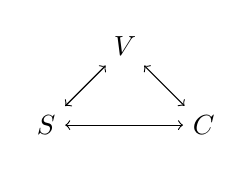
\begin{tikzpicture}
\node (V) at (0,1) {$V$};
\node (S) at (-1,0) {$S$};
\node (C) at (1,0) {$C$};
\draw[<->] (V) to (S);
\draw[<->] (S) to (C);
\draw[<->] (C) to (V);
\end{tikzpicture}}}
\end{equation}
其中 $V$、$S$、$C$ 是 $\SO(8)$ 的八维不可约表示，分别为矢量、旋量和共轭旋量表示。这三个八维不可约表示之间的交换由外自同构诱导，称为群 $\SO(8)$ 的三重性；其 Dynkin 图也画在图 \ref{fig:triality} 中。这一三重性最初由文献 \cite{Seiberg:1994aj} 发现。本小节的论述遵循文献 \cite{Gaiotto:2009we}。

这一系统的希格斯支可以在任一种描述中研究。原来有超多重态 $q_I^a$，其中 $a=1,2$、$I=1,\ldots,8$。规范不变组合为
\begin{equation}
M_{[IJ]}=q_I^aq_J^b\epsilon_{ab}.
\end{equation}
在对偶理论中，有超多重态 $\tilde q^{\tilde a}_{\tilde I}$，其中 $\tilde a=1,2$ 对应对偶 $\SU(2)$，而 $\tilde I=1,\ldots,8$ 对应 $\SO(8)$ 味对称性的旋量表示。此时基本的规范不变量为
\begin{equation}
\tilde M_{[\tilde I\tilde J]}=\tilde q^{\tilde a}_{\tilde I}\tilde q^{\tilde b}_{\tilde J}\epsilon_{\tilde a\tilde b}.
\end{equation}
$M_{[IJ]}$ 和 $\tilde M_{[\tilde I\tilde J]}$ 都处于 $\SO(8)$ 的伴随表示中，可以利用 $\SO(8)$ 的外自同构自然地将它们对应起来。可以检验，$M_{[IJ]}$ 和 $\tilde M_{[\tilde I\tilde J]}$ 满足的约束在外自同构下不变。这表明，希格斯支作为复空间是相同的。
\subsection{推广}\label{sec:trivalent}
\subsubsection{三价图}\index{TrivalentDiagram@三价图|hyperpage}
\begin{figure}[h]
\[
\inc{trivalent}
\]
\caption{三价图及其对应的紫外曲线。\label{fig:trivalent}}
\end{figure}
由 $\cN{=}1$ 手征多重态 $q_{a\alpha u}$（$a,\alpha,u=1,2$）组成的三基本表示超多重态，在迄今的分析中起到了核心作用。我们为它引入一种简记法：如图 \ref{fig:trivalent} 所示，用带有标记 $A$、$B$、$C$ 的三价顶点表示它，分别代表作用于指标 $a$、$\alpha$、$u$ 的对称性 $\SU(2)_A$、$\SU(2)_B$、$\SU(2)_C$。

这一系统的紫外曲线是带有三个穿孔 $A$、$B$、$C$ 的球面，Seiberg-Witten 曲线为
\begin{equation}
\Sigma:\qquad\lambda^2-\phi(z)=0
\end{equation}
其中 $\phi(z)$ 由如下条件确定：在各穿孔 $A,B,C$ 处，二阶极点的系数分别为 $\mu_A^2$、$\mu_B^2$、$\mu_C^2$，如式 \eqref{phicondition_trifund} 所示。

现在，取两个三基本表示超多重态，并将一个 $\SU(2)$ 规范多重态耦合到它们，就可以得到含有四个味的 $\SU(2)$ 理论。我们用两个三价顶点以及连接它们的一条线来表示这一理论，如图 \ref{fig:trivalent} 所示。在连接线上标出指数化耦合 $q$。

从这一三价图出发，很容易写出理论的拉格朗日量。理论的自由参数是质量参数 $\mu_{A,B,C,D}$ 和紫外耦合 $q$。这一系统的紫外曲线是带有四个穿孔 $A$、$B$、$C$、$D$ 的球面，Seiberg-Witten 曲线为
\begin{equation}
\Sigma:\qquad\lambda^2-\phi(z)=0
\end{equation}
其中 $\phi(z)$ 由各穿孔 $X=A,B,C,D$ 处的留数为 $\mu_X^2$ 这一条件确定，如式 \eqref{so8masses} 所示。图 \ref{fig:triality} 已经展示了含有四个味的 $\SU(2)$ 理论的三重性；用三价图可以将其画成图 \ref{fig:triality-trivalent} 的形式。

\begin{figure}[h]
\[
\inc{triality-trivalent}
\]
\caption{用三价图表示的三重性。\label{fig:triality-trivalent}}
\end{figure}

这样，我们可以将三价图视为表示紫外拉格朗日量的简记法。对于给定的这一紫外拉格朗日理论，只需将每个三价顶点替换为一个三穿孔球面，将每条连接线替换为一根连接管，就能得到它的 Seiberg-Witten 解。这是一种出人意料地简洁的、求取 $\cN{=}2$ 规范理论的 Seiberg-Witten 解的方法。

\subsubsection{例：带有一个穿孔的环面}\index{NTwoStarTheory@$\cN{=}2^*$ 理论|hyperpage}\index{WeierstrassFunction@Weierstraß 函数|hyperpage}\index{ModularGroup@模群|hyperpage}
\begin{figure}[h]
\[
\inc{trivalent-n2star}
\]
\caption{含有伴随表示超多重态以及一个自由超多重态的 $\SU(2)$ 理论。\label{fig:n2star}}
\end{figure}
我们来看几个例子。首先，取一个三价顶点，用一条边连接三条线中的两条，见图 \ref{fig:n2star}。我们从由 $\cN{=}1$ 手征多重态 $q_{a\alpha u}$ 描述的三基本表示出发，不过将同一个 $\SU(2)$ 规范多重态耦合到指标 $a$ 和 $\alpha$。于是，组合 $(a,\alpha)$ 处于两个自旋 $1/2$ 表示的张量积中。因此，可以将它分解为一个三重态和一个单态，并带有额外的指标 $u=1,2$：
\begin{equation}
q_{a\alpha u}\to q'_{iu},q''_u,
\end{equation}
其中 $i=1,2,3$ 是 $\SU(2)$ 三重态的指标。

总之，我们只有一个处于三重态中的完整超多重态，以及另一个处于单态中、完全退耦的完整超多重态。因此，这本质上就是 $\cN{=}2^*$ $\SU(2)$ 理论，等价地说，就是对伴随表示超多重态作了质量形变的 $\cN{=}4$ $\SU(2)$ 理论。伴随表示的质量 $\mu$ 与剩下的一个 $\SU(2)$ 味对称性相联系。

用一根管连接三穿孔球面上的两个穿孔，即可得到它的 Seiberg-Witten 解。如图 \ref{fig:n2star} 所示，紫外曲线是带有一个穿孔的环面。此时 Seiberg-Witten 曲线为
\begin{equation}
\lambda^2-\phi(z)=0
\end{equation}
其中 $z$ 现在是环面上的坐标；我们将环面视为施加了等同关系 $z\sim z+1\sim z+\tau$ 的复平面。由于坐标原点可以任意选择，我们将穿孔放在原点。$\phi(z)$ 由如下条件确定：它在 $z=0$ 处有一个给定强度的二阶极点。这一条件将 $\phi(z)$ 的形式唯一确定为
\begin{equation}
\phi(z)=(\mu^2\wp(z;\tau)+u)dz^2
\end{equation}
其中 $\wp$ 是 Weierstra\ss\ 函数，$u$ 是库仑支真空期望值 $u=\vev{\tr\Phi^2}/2$。

现在很清楚，交换单极子与伴随表示夸克之后，耦合由 $\tau$ 给定的理论，与耦合由 $\tau'=-1/\tau$ 给定的同一理论是等价的。耦合空间可以与环面、即亏格为 $1$ 的黎曼曲面的模空间 $\cM_1$ 对应起来，后者为
\begin{equation}
\cM_1=\bH/\SL(2,\bZ)\label{SL2Zfund}
\end{equation}
其中 $\bH$ 是 $\tau$ 取值的上半平面，$\SL(2,\bZ)$ 是交换环面各边的模群。对偶群可以与模群对应起来。

\subsubsection{例：带有五个穿孔的球面}
\begin{figure}[h]
\[
\inc{trivalent-tree}
\]
\caption{一个 $\SU(2)^2$ 理论及其曲线。\label{fig:su2-quiver}}
\end{figure}
再看一个例子：取三个三价顶点，按图 \ref{fig:su2-quiver} 所示的方式将它们连接起来。最左边的三价顶点对于 $\SU(2)_1$ 而言相当于 $N_f=2$ 个味，最右边的三价顶点对于 $\SU(2)_2$ 而言相当于 $N_f=2$ 个味。此外，还有一个来自中央三价顶点的超多重态 $q_{aiu}$，其中 $a$ 对应 $\SU(2)_1$，$i$ 对应 $\SU(2)_2$。剩下的指标 $u=1,2$ 是味对称性的指标。较早的文献更习惯于使用 $\cN{=}1$ 手征多重态 $(Q^i_a,\tilde Q_i^a)$ 来表示这一在 $\SU(2)_1\times\SU(2)_2$ 下带荷的超多重态，其中
\begin{equation}
Q^i_a=q_{aju=1}\epsilon^{ij},\qquad
\tilde Q_i^a=q_{biu=2}\epsilon^{ab}.
\end{equation}
它通常称为在 $\SU(2)_1\times\SU(2)_2$ 下带荷的双基本表示多重态。

这一理论的 Seiberg-Witten 解很容易求得，如图 \ref{fig:su2-quiver} 所示。我们从三个球面出发，分别用复坐标 $z_1$、$z_2$、$z_3$ 描述。穿孔 $A,B$ 位于 $z_1=0,1$；穿孔 $C$ 位于 $z_2=1$；穿孔 $D,E$ 分别位于 $z_3=1,\infty$。为了连接 $z_1=\infty$ 与 $z_2=0$，引入 $w_1=1/z_1$，并要求满足关系 $w_1z_2=q'$。这就意味着有 $z_1=q'z_2$。类似地，连接 $z_2=\infty$ 与 $z_3=0$，就有 $z_2=qz_3$。现在引入 $z=z_3$，用来描述所得到的五穿孔球面上的坐标。于是，各穿孔位于 $z=0$、$qq'$、$q$、$1$ 和 $\infty$，每个穿孔都代表一个 $\SU(2)$ 味对称性，分别记作 $\SU(2)_{A,B,C,D,E}$。$\SU(2)_1\times\SU(2)_2$ 的规范耦合可以与 $q$ 和 $q'$ 对应起来。

将与各味对称性相联系的质量参数记为 $\mu_{A,B,C,D,E}$。Seiberg-Witten 曲线为
\begin{equation}
\lambda^2-\phi(z)=0
\end{equation}
其中 $\phi(z)$ 需要满足渐近行为
\begin{equation}
\phi(z)\sim\frac{\mu_X^2}{z_X^2}dz_X^2\label{massive-full-su2}
\end{equation}
其中，对于 $X=A,B,C,D,E$，$z_X$ 是紫外曲线上的局部坐标，使穿孔 $X$ 位于 $z_X=0$。由 $A$、$B$、$C$、$D$ 处的条件可知，$\phi$ 为
\begin{equation}
\phi(z)=\frac{P(z)}{z^2(z-1)^2(z-q)^2(z-qq')^2}dz^2
\end{equation}
其中 $P(z)$ 是一个多项式。为了施加 $E$ 处的条件，换用坐标 $w=1/z$。要使 $\phi(z)$ 的行为为 $\sim dw^2/w^2$，$P(z)$ 的最高次项只能到 $z^6$。因此，$\phi(z)$ 有七个系数。其中五个组合是质量参数，而不改变二阶极点系数的两个线性组合，则是两个规范多重态 $\SU(2)_{1,2}$ 的库仑支参数 $u=\vev{\tr\Phi^2}/2$ 和 $u'=\vev{\tr\Phi'{}^2}/2$。从 Seiberg-Witten 解可以看出，这一理论具有强弱耦合对偶：只要适当改变两个规范群的耦合 $(q,q')$，就可以任意置换五个味对称群 $\SU(2)_{A,B,C,D,E}$。这一推广的对偶最初由文献 \cite{Argyres:1999fc} 发现。

\subsubsection{例：亏格为二的曲面}\index{MappingClassGroup@映射类群|hyperpage}\index{TeichmullerSpace@Teichmüller 空间|hyperpage}
\begin{figure}[h]
\[
\inc{trivalent-genus2}
\]
\caption{两个 $\SU(2)^3$ 理论及其曲线。\label{fig:genus-2}}
\end{figure}
作为第三个例子，取两个三价顶点，用三条边将它们连接起来。这可以通过两种拓扑上不同的方式实现，如图 \ref{fig:genus-2} 左侧所示。

上方的理论是一个 $\SU(2)_l\times\SU(2)_m\times\SU(2)_r$ 规范理论。它含有处于
\begin{equation}
\mathbf{3}\otimes\mathbf{2}\otimes\mathbf{1},\qquad
\mathbf{1}\otimes\mathbf{2}\otimes\mathbf{3}
\end{equation}
表示中的半超多重态，以及一个在 $\SU(2)_m$ 下带荷的完整超多重态。注意，三价图构造不允许我们考虑最后这个完整超多重态具有非零质量项的理论。下方的理论是一个 $\SU(2)_1\times\SU(2)_2\times\SU(2)_3$ 理论，含有两个三基本表示半超多重态。同样，三价图构造不允许我们为这个三基本表示完整超多重态引入非零质量项。

Seiberg-Witten 解同样很容易得到。为了得到紫外曲线，将两个三价顶点替换为三穿孔球面，再用管将穿孔两两连接起来。可以看到，这两种情形得到的都是光滑的亏格为 $2$ 的曲面。Seiberg-Witten 曲线则是进一步的二重覆盖，由
\begin{equation}
\lambda^2-\phi(z)=0
\end{equation}
给出，其中 $z$ 是亏格为 $2$ 的曲面上的复坐标，$\phi(z)$ 是其上的光滑二次微分。固定亏格为 $2$ 的曲面上的二次微分空间具有三个复维度，我们将它们与库仑支真空期望值 $u_i=\vev{\tr\Phi_i^2}/2$ 对应起来。

现在很清楚，通过调节规范耦合，可以将上方的理论连续地形变为下方的理论。非微扰的耦合空间可以与亏格为 $2$ 的黎曼曲面的模空间 $\cM_2$ 对应起来；该模空间具有三个复维度。对偶群对应于亏格为 $2$ 的曲面的映射类群 $\cG_2$，且 $\cM_2=\cT_2/\cG_2$，其中 $\cT_2$ 是亏格为 $2$ 的黎曼曲面的 Teichm\"uller 空间；可与亏格为 $1$ 的情形式 \eqref{SL2Zfund} 比较。

一个多少有些令人惊讶的数学事实是：$\cT_2$ 在光滑意义下等价于上半平面的三个副本 $\bH^3$，但在全纯意义下并不等价\footnote{作者感谢 Jacques Distler 就这一点所作的极富启发性的讨论。}：
\begin{equation}
\begin{aligned}
\cT_2\simeq\bH^3&\quad\text{在光滑意义下},\\
\cT_2\not\simeq\bH^3&\quad\text{在全纯意义下}.
\end{aligned}
\end{equation}
朴素的微扰分析告诉我们，$\SU(2)^3$ 的耦合空间就是上半平面的三个副本：
\begin{equation}
(\tau_1,\tau_2,\tau_3)\in\bH^3
\end{equation}
而且复结构也包括在内。因此，我们发现，非微扰修正能够使超对称理论参数空间的复结构发生相当剧烈的变化。

\subsubsection{曲线与 Hitchin 场}\label{sec:hitchin}\index{HitchinField@Hitchin 场|hyperpage}\index{HitchinSystem@Hitchin 系统|hyperpage}
我们已经知道，将 Seiberg-Witten 曲线写成
\begin{equation}
\Sigma:\qquad\lambda^2-\phi(z)=0\label{prehitchin}
\end{equation}
的形式，对理解系统很有帮助。曲线的这种表示方式与紫外曲线 $C$ 上所谓的 Hitchin 系统密切相关。对这一技巧的讲解足以另成一份讲义。读者可以从例如文献 \cite{Gaiotto:2009hg} 第 3 节开始了解。

我们至少来非常粗略地介绍它的一个方面。考虑一个无迹的 $2\times2$ 矩阵值亚纯一形式 $\varphi(z)$。于是，可以对一形式 $\lambda$ 构造如下形式的方程：
% [Tutor Note: p.105 原文 "We consider a meromoprhic one-form $\varphi(z)$" 中 "meromoprhic" 应为 "meromorphic"，系拼写笔误；译文按其本意作“亚纯一形式”。]
\begin{equation}
\det(\lambda-\varphi(z))=0.\label{hitchin}
\end{equation}
将式 \eqref{prehitchin} 与式 \eqref{hitchin} 对应起来，得到
\begin{equation}
\frac12\tr\varphi(z)^2=\phi(z).\label{p-p}
\end{equation}
这一矩阵场 $\varphi(z)$ 称为 Hitchin 场\footnote{Hitchin 本人将 $\varphi(z)$ 称为希格斯场，但作者认为，在 $\cN{=}2$ 超对称语境中，这一术语颇易引起混淆，因为 $\varphi(z)$ 控制的是库仑支的物理，而不是希格斯支的物理。}。可以利用弦对偶来理解为何紫外曲线上存在这样一个复的伴随表示场，不过对它的解释超出了本讲义的目的。

在与质量项 $\mu_X$ 相联系、位于 $z_X=0$ 的穿孔处，场 $\phi(z)$ 的条件已在式 \eqref{massive-full-su2} 中给出：
\begin{equation}
\phi(z)=\mu_X^2\frac{dz_X^2}{z_X^2}+\text{（奇异性较弱的项）}.\label{phi-full}
\end{equation}
它转化为 Hitchin 场 $\varphi(z)$ 的条件
\begin{equation}
\varphi(z)\sim\begin{pmatrix}
\mu_X&0\\
0&-\mu_X
\end{pmatrix}\frac{dz_X}{z_X}+\text{（奇异性较弱的项）}.\label{varphi-full}
\end{equation}
这里，符号 $A\sim B$ 表示 $A$ 与 $B$ 共轭，也就是说，存在可逆的 $N\times N$ 复矩阵 $g$，使得 $A=gBg^{-1}$。

现在，考虑将 $\mu_X$ 关掉、令其为零时会发生什么。在式 \eqref{phi-full} 的描述中，边界条件变为
\begin{equation}
\phi(z)=c\frac{dz_X^2}{z_X}+\text{（奇异性较弱的项）}\label{q-q}
\end{equation}
其中 $c$ 是某个常数。而在式 \eqref{varphi-full} 的描述中，留数并不是简单地变成零矩阵。注意，只要 $\mu_X\neq0$，就有
\begin{equation}
\begin{pmatrix}
\mu_X&0\\
0&-\mu_X
\end{pmatrix}
\sim
\begin{pmatrix}
\mu_X&1\\
0&-\mu_X
\end{pmatrix},
\end{equation}
而且可以在右侧取极限 $\mu_X\to0$。这意味着，无质量极限给出的边界条件具有如下形式：
\begin{equation}
\varphi(z)\sim\begin{pmatrix}
0&1\\
0&0
\end{pmatrix}\frac{dz_X}{z_X}+\text{（奇异性较弱的项）}.
\end{equation}
利用式 \eqref{p-p}，可以发现它重现了条件 \eqref{q-q}。

在这一阶段，使用 $\varphi(z)$ 而不是 $\phi(z)$ 的优点可能还不太明显。然而，当我们讨论推广到 $\SU(N)$ 规范理论，或具有更复杂规范群的规范理论时，它就会变得至关重要。
% [Tutor Note: p.106 原文 "one might not find the advantange of using $\varphi(z)$ instead of $\phi(z)$ very much" 中 "advantange" 应为 "advantage"；同段 "It turns out, however, that … it turns out to be crucial" 重复了 "turns out"。两处均为笔误，译文按本意译出。]

\subsection{再论味数较少的理论}\label{sec:less}\index{WildPuncture@野性穿孔|hyperpage}
我们发现，将 $N_f=4$ 理论的 Seiberg-Witten 曲线写成
\begin{equation}
\lambda^2-\phi(z)=0
\end{equation}
的形式，极大地有助于理解对偶的结构。现在将这一思想应用于味数较少、即 $N_f<4$ 的理论的曲线。

\subsubsection{曲线的改写}
首先，考虑纯理论的曲线，
\begin{equation}
\frac{\Lambda^2}z+\Lambda^2z=x^2-u,\qquad\text{其中}\ \lambda=x\frac{dz}z.
\end{equation}
用 $\lambda$ 可以将它写成
\begin{equation}
\lambda^2-\phi(z)=0,\qquad\phi(z)=(\frac{\Lambda^2}z+u+\Lambda^2z)\frac{dz^2}{z^2}.
\end{equation}
可以看到，二次微分 $\phi(z)$ 的奇异性比 $N_f=4$ 理论中的更强：现在它在 $z=0$ 和 $=\infty$ 处具有三阶极点。曲线的情形可以画成图 \ref{fig:lessG} 上排的样子。其中，罗马数字 III 表示 $\phi(z)$ 在该穿孔处具有三阶极点。$\phi(z)$ 的高阶极点奇异性构成了一类新的穿孔，我们将它们称为野性 $\SU(2)$ 穿孔。

作为编码紫外拉格朗日量的三价图的推广，我们引入如下记号：一条边代表一个 $\cN{=}2$ $\SU(2)$ 矢量多重态，而一端的黑色方块表示不引入任何超多重态。于是，很容易看出从表示紫外拉格朗日量的图到紫外曲线的转换关系，如图 \ref{fig:lessG} 所示。
\begin{figure}[h]
\[
\inc{trivalent-lessflavorsXX}
\]
\caption{味数较少的 $\SU(2)$ 理论。\label{fig:lessG}}
\end{figure}
其次，考虑 $N_f=1$ 理论的曲线，
\begin{equation}
\frac{2\Lambda(\tilde x-\mu)}z+\Lambda^2z=\tilde x^2-u,\qquad\text{其中}\ \tilde\lambda=\tilde x\frac{dz}z.
\end{equation}
它可以写成
\begin{equation}
\lambda^2-\phi(z)=0,\qquad\phi(z)=(\frac{\Lambda^2}{z^2}-\frac{2\Lambda\mu}z+u+\Lambda^2z)\frac{dz^2}{z^2}
\end{equation}
其中 $\lambda=xdz/z$ 由 $\tilde\lambda$ 平移而来。我们发现，$z=0$ 处的奇点变成了四阶极点。拉格朗日量及其 Seiberg-Witten 解可以简洁地概括为图 \ref{fig:lessG} 下排的形式。边代表一个 $\SU(2)$ 规范群。一端的黑色方块表示那里没有任何超多重态。另一端的浅色圆点表示引入一个二重态超多重态。将黑色方块对应于一个带有三阶极点、用 III 标记的球面，类似地将浅色圆点对应于一个带有四阶极点、用 IV 标记的球面，最后用一根管将它们连接起来，即可得到解。注意，四阶极点具有自己的 $\SU(2)$ 味对称性和相应的质量参数。

总之，我们将带有一个正则穿孔和一个极点阶数为 III 的野性穿孔的球面视为空理论，将带有一个正则穿孔和一个极点阶数为 IV 的野性穿孔的球面视为退耦的二重态超多重态理论，如图 \ref{fig:lessG} 所示。用管连接正则穿孔，就得到味数较少的理论的紫外曲线。

\subsubsection{推广}
\begin{figure}[h]
\[
\inc{trivalent-mixedX}
\]
\caption{一个 $\SU(2)^4$ 理论及其曲线。\label{fig:complicated-example}}
\end{figure}
这一推广使我们能够求出一大类 $\cN{=}2$ 理论的 Seiberg-Witten 解，其规范群是若干个 $\SU(2)$ 的乘积。例如，考虑图 \ref{fig:complicated-example} 左侧描述的、规范群为 $\SU(2)^4$ 的紫外拉格朗日理论。用文字来说，我们先取三个双基本表示超多重态，
\begin{equation}
Q_{aiu},\quad Q'_{us\alpha},\quad Q''_{\alpha xm}.
\end{equation}
图中展示了如何将各指标分配到三价图的边上。对应于动力学规范群的边用粗线突出表示。用文字来说，指标 $a,i,m$ 对应于 $\SU(2)_{A,B,C}$ 味对称性。一个 $\SU(2)$ 规范多重态耦合到指标 $u$，指数化耦合常数为 $q$；另一个 $\SU(2)$ 规范多重态耦合到指标 $\alpha$，指数化耦合常数为 $q'$。再引入一个 $\SU(2)_1$ 规范多重态，使其耦合到黑色方块所对应的指标 $s$；最后再引入一个 $\SU(2)_2$ 规范多重态，使其耦合到指标 $x$，并额外带有 $N_f=1$ 个超多重态 $(Q''''{}_x,\tilde Q''''{}^x)$。必要时我们可以写出拉格朗日量，但现在已经可以看出，三价图对其结构的概括是多么简洁。

它的 Seiberg-Witten 解可以立即得到，由
\begin{equation}
\lambda^2-\phi(z)=0,
\end{equation}
给出，其中 $\phi(z)$ 有三个二阶极点、一个三阶极点，以及一个四阶极点。分别将它们放在 $z=0,1,z_0$、$z_1$ 和 $\infty$ 处，可以看到 $\phi(z)$ 具有形式
\begin{equation}
\phi(z)=\frac{P(z)}{z^2(z-1)^2(z-z_0)^2(z-z_1)^3}dz^2
\end{equation}
其中 $P(z)$ 是一个多项式。要在 $w=1/z=0$ 处具有四阶极点，$P(z)$ 必须是九次多项式。在十个系数中，三个是 $\SU(2)_{A,B,C}$ 味对称性的质量参数，一个是黑色圆点所对应的 $\SU(2)_1$ 的能标，一个是 $\SU(2)_2$ 的能标，还有一个是 $\SU(2)_2$ 的额外 $N_f=1$ 个味的质量参数。剩下的四个线性组合可以与四个库仑支参数 $u_i=\vev{\tr\Phi_i^2/2}$ 对应起来。这不是一个共形理论：它具有两个动力学能标 $\Lambda$ 和 $\Lambda'$。尽管如此，从紫外曲线的结构仍然可以立即看出，存在交换 $A$、$B$、$C$ 处三个正则穿孔的 S 对偶。

\section{Argyres-Douglas 共形场论}\label{sec:AD}\index{ArgyresDouglasCFT@Argyres-Douglas 共形场论|hyperpage}\index{ArgyresDouglasPoint@Argyres-Douglas 点|hyperpage}\index{ScalingDimension@标度维数|hyperpage}
本节回到第 \ref{sec:nf_1_curve} 小节末尾的观察：$N_f=1$ 理论的库仑支上存在一个高度奇异的点。我们将研究该点的物理及其推广。

\subsection{$N_f=1$ 理论与最简单的 Argyres-Douglas 共形场论}
再次回到含有 $N_f=1$ 个味的 $\SU(2)$ 规范理论的曲线：
\begin{equation}
\Sigma:\quad\frac{2\Lambda(x-\mu)}z+\Lambda^2z=x^2-u.\label{nf1curveagain}
\end{equation}
对于一般的 $\Lambda$ 和 $\mu$，$u$ 平面上有三个奇点。正如第 \ref{sec:nf_1_curve} 小节末尾所见，当取 $\mu=-\frac32\Lambda$ 时，两个奇点在 $u=3\Lambda^2$ 处碰撞，见图 \ref{fig:nf_1_adpoint}。
\begin{figure}[h]
\[
\inc{ADnf1X}
\]
\caption{$N_f=1$ 理论的 Argyres-Douglas 点。\label{fig:nf_1_adpoint}}
\end{figure}
当 $u\sim3\Lambda^2$ 时，$x(z)$ 的三个分支点在 $z=-1$ 处碰撞。此时，定义 $a$ 和 $a_D$ 的 $A$ 闭链与 $B$ 闭链，都可以取为环绕 $z=0$ 的小环路。这保证了 $a$ 和 $a_D$ 都很小。因此，我们同时具有很轻的电荷粒子和磁荷粒子。库仑支上的这种点称为 Argyres-Douglas 点。文献 \cite{Argyres:1995jj} 首先在纯 $\SU(3)$ 理论中识别出了这样的点，文献 \cite{Argyres:1995xn} 又将其推广到含有味的 $\SU(2)$ 理论。

% [Tutor Note: p.109 原文 "small loops around $z=0$" 中的 $z=0$ 应为 $z=-1$：同一段前一句刚说明三个分支点在 $z=-1$ 处碰撞，围绕这些分支点的小环路应取在 $z=-1$ 附近（v3 版已改作 $z=-1$，可作旁证）。正文照原文排 $z=0$。]

环绕 $u=3\Lambda^2$ 的单值变换 $M_{AD1}$ 可以用多种方法求得。一种方法是将 $N_f=1$ 理论中两个相碰奇点的单值变换相乘。另一种方法是追踪三个分支点的运动。令 $u=3\Lambda^2+\delta u$，可得三个分支点位于 $z+1\propto\delta u^{1/3}$ 处。这就确定了闭链如何被映射，从而得到单值变换。无论使用哪种方法，都有
\begin{equation}
M_{AD1}\sim\begin{pmatrix}
1&1\\
-1&0
\end{pmatrix}.
\end{equation}
$M_{AD1}$ 对低能耦合的变换为
\begin{equation}
\tau\mapsto\tau'=\frac1{1-\tau}.
\end{equation}
注意，$\tau=e^{\pi i/3}$ 是这一变换的不动点；通过显式计算，可以检验 $\tau-e^{\pi i/3}\propto\delta u^{1/3}$。我们发现，耦合被固定在这一强耦合值上。

人们认为，低能极限是共形的。为了分离出这一极限中的物理，令
\begin{equation}
\begin{aligned}
z&=-1+\tilde\delta z,&
x&=-\Lambda+\Lambda\delta x,&
u&=3\Lambda^2+\Lambda^2\tilde\delta u,&
\mu&=-\frac32\Lambda+\Lambda\tilde\delta\mu.
\end{aligned}
\end{equation}
并假定所有以 $\delta$ 为前缀的变量都很小。事实表明，进一步引入如下重定义更加有用：
\begin{equation}
\tilde\delta z=\delta z-(\delta z)^2,\quad
\tilde\delta u=\delta u-2\delta\mu-2\delta x+(\delta z)^2,\quad
\tilde\delta\mu=\delta\mu+\delta x.\label{ADredefinition1}
\end{equation}

现在，将关系 \eqref{ADredefinition1} 代入 $N_f=1$ 曲线 \eqref{nf1curveagain}。展开到 $\delta z$ 的三阶，得到如下形式的曲线：
\begin{equation}
(\delta x)^2-\delta u=-(\delta z)^3+2\delta\mu\delta z.\label{nf1ADcurve}
\end{equation}
微分为
\begin{equation}
\lambda=x\frac{dz}z\sim\delta x d\delta z.
\end{equation}
由于积分 $\int\lambda$ 给出 BPS 粒子的质量，$\lambda$ 本身应具有标度维数 $1$。关系 \eqref{nf1ADcurve} 意味着，标度维数 $[\delta x]$ 与 $[\delta z]$ 应满足
\begin{equation}
[\delta x]:[\delta z]=3:2.
\end{equation}
这就固定了所有相关变量的标度维数：
\begin{equation}
[\delta x]=\frac35,\qquad[\delta x]=\frac25,\qquad
[\delta u]=\frac65,\qquad[\delta\mu]=\frac45.
\end{equation}
% [Tutor Note: p.110 式 (10.1.9) 原文第二个 $[\delta x]$ 应为 $[\delta z]$：上一式给出 $[\delta x]:[\delta z]=3:2$，下面两式依次使用 $[\delta x]=3/5$、$[\delta z]=2/5$、$[\delta u]=6/5$、$[\delta\mu]=4/5$（v3 版已改作 $[\delta z]$，可作旁证）。正文照原文排。]
注意，算符 $u=\tr\Phi^2/2$ 的质量量纲，等价地说，它在紫外的标度维数，原本是 $2$。我们发现，反常维数是 $1$ 的量级，使 $[\delta u]$ 显著减小。

\begin{figure}[h]
\[
\inc{AD1}
\]
\caption{Argyres-Douglas 理论 $AD_{N_f=1}(\SU(2))$。\label{fig:H1}}
\end{figure}
在取极限 $\delta u\to0$ 时，我们是在放大 $u$ 平面上 $u=3\Lambda^2$ 附近的邻域。在这一极限中，可以认为低能理论由一个仅在 $\delta u=0$ 处具有奇点的理论描述，如图 \ref{fig:H1} 左侧所示。我们将得到的理论称为 Argyres-Douglas 共形场论 $AD_{N_f=1}(\SU(2))$\footnote{遗憾的是，文献中对于 Argyres-Douglas 理论还没有公认的统一命名体系。本讲义试图提供一种命名体系，它可能比文献中的命名更加繁琐，但在区分各种构造时更加明确。}。

从六维观点重新考察这一取极限的过程。首先，将原来的 $N_f=1$ 曲线写成 $\lambda^2-\phi(z)=0$ 的形式。回顾第 \ref{sec:less} 小节的研究以及图 \ref{fig:lessG}，$\phi(z)$ 有一个三阶极点和一个四阶极点。此外，在一般位置上还有 $\phi(z)$ 的三个分支点。假定仔细调节参数，使 $\phi(z)$ 的两个极点碰撞：
\begin{equation}
\phi(z)\sim(\frac{P_3(z)}{(z-\epsilon)^3}+\frac{P_4(z)}{z^4})dz^2
=\frac{P_7(z)}{(z-\epsilon)^3z^4}dz^2
\to\frac{Q_7(z)}{z^7}dz^2
\end{equation}
其中，在这一阶段，$P_d$、$Q_d$ 是一般的 $d$ 次多项式。最终只剩下一个具有七阶极点的奇点，如图 \ref{fig:H1} 右侧所示。为了在 $z=\infty$ 处没有奇点，$Q_7(z)$ 实际上应当是三次多项式：
\begin{equation}
\lambda^2=\frac{c+c'z+\mu z^2+uz^3}{z^7}dz^2.
\end{equation}
通过坐标变换 $z\to z/(az-b)$，可以令 $c=1$、$c'=0$。于是有
\begin{equation}
\lambda^2=\frac{1+\mu z^2+uz^3}{z^7}dz^2.
\end{equation}
由于左侧的标度维数为 $2$，可得 $[z]=-2/5$，从而有
\begin{equation}
[\mu]=\frac45,\qquad[u]=\frac65\label{muu}
\end{equation}
这与前面的结果一致。注意，变量 $z$ 是辅助变量，因此没有理由要求它的维数与前面相同。

一般而言，对于任意共形场论，任意动力学标量算符 $O$ 都应具有大于或等于 $1$ 的标度维数：
\begin{equation}
[O]\ge1,\label{generalCFTfeatures}
\end{equation}
而且只有当 $O$ 描述一个自由、退耦的标量玻色子时，等号才能成立。因此，具有 $[u]=6/5$ 的算符 $u$ 是理论 $AD_{N_f=1}(\SU(2))$ 中的真正算符。$\mu$ 则在如下意义下被视为与 $u$ 共轭的参数。在 $\cN{=}2$ 理论中，可以考虑预势的形变
\begin{equation}
\int d^4\theta F\to\int d^4\theta(F+mO).
\end{equation}
这里，$d^4\theta$ 是第 \ref{sec:lel} 小节末尾简要提到的手征 $\cN{=}2$ 超空间积分，$O$ 是一个算符，$m$ 是乘在它前面的参数。因此，在 $\cN{=}2$ 超共形理论中，组合 $mO$ 需要具有标度维数 $2$。于是应有
\begin{equation}
[m]+[O]=2.
\end{equation}

可以看到，$\mu$ 与 $u$ 这一对满足此条件，见式 \eqref{muu}。因此，我们将 $\mu$ 视为对应于算符 $u$ 的形变参数。

\subsection{来自 $N_f=2$ 理论的 Argyres-Douglas 共形场论}\index{MassParameter@质量参数|hyperpage}
考虑 $N_f=2$ 理论的曲线，
\begin{equation}
\frac{2\Lambda(x-\mu)}z+2\Lambda(x-\mu)z=x^2-u\label{firstform}
\end{equation}
其中令两个味的质量相同。也可以使用另一种形式的曲线
\begin{equation}
\frac{(x-\mu)^2}z+4\Lambda^2z=x^2-u.\label{secondform}
\end{equation}
对于一般的 $\mu$，其模空间已经画在图 \ref{fig:nf_2_moduli} 中。

当 $\mu=0$ 时，两个没有连接希格斯支的奇点发生碰撞。现在，转而调节参数 $\mu$，使带有希格斯支的奇点与一个不带希格斯支的奇点碰撞，见图 \ref{fig:nf_2_AD_plane}。为了明确起见，使用曲线的第一种形式。此时，碰撞发生在 $\mu=2\Lambda$、$u=4\Lambda^2$ 时。四个分支点随后在 $z=1$ 处碰撞。
\begin{figure}[h]
\[
\inc{ADnf2X}
\]
\caption{$N_f=2$ 理论的 Argyres-Douglas 点。\label{fig:nf_2_AD_plane}}
\end{figure}
我们发现，环绕所得到奇点的单值变换为
\begin{equation}
M_{AD2}\sim\begin{pmatrix}
0&1\\
-1&0
\end{pmatrix},
\end{equation}
它对耦合的作用为
\begin{equation}
\tau\to\tau'=-\frac1\tau.
\end{equation}
强耦合值 $\tau=i$ 是这一变换的不动点，当令 $u\to4\Lambda^2$ 时，低能耦合趋近于这一值。

与前面一样展开各变量，
\begin{equation}
\begin{aligned}
z&=1+\delta z,&
x&=2\Lambda+\delta x,&
u&=4\Lambda^2+\delta u,&
\mu&=2\Lambda+\delta\mu,
\end{aligned}
\end{equation}
可得极限中的曲线为
\begin{equation}
(\delta x)^2+\delta u=(\delta z)^4+\delta\mu\delta z^2+\Delta\mu\delta z\label{nf2ADcurve}
\end{equation}
微分为 $\lambda\sim\delta x d\delta z$。这里，重新引入了两个二重态超多重态的裸质量 $\mu_1$、$\mu_2$ 之间的微小差值 $\Delta\mu=\mu_1-\mu_2$。要求 $\lambda$ 的标度维数为 $1$，便有
\begin{equation}
[\delta x]=\frac23,\quad[\delta z]=\frac13.
\end{equation}
于是得到
\begin{equation}
[\delta u]=\frac43,\quad[\delta\mu]=\frac23,\quad[\Delta\mu]=1.\label{scalingdimH2}
\end{equation}
再次可见，$[\delta u]+[\delta\mu]=2$，因此 $\delta\mu$ 是对应于算符 $\delta u$ 的形变参数。$\Delta\mu$ 是非阿贝尔味对称性 $\SU(2)_F$ 的质量参数。一般而言，在共形理论中，非阿贝尔味对称流 $J^a$ 应具有标度维数 $3$。$\cN{=}2$ 超对称性将它与质量项联系起来；对于拉格朗日理论，这个质量项就是熟悉的 $Q\tilde Q$，具有标度维数 $2$。因此，$\cN{=}2$ 超共形理论的非阿贝尔质量参数始终应具有标度维数 $1$。我们对 $[\Delta\mu]$ 的计算与这一一般论证一致。将得到的理论称为 $AD_{N_f=2}(\SU(2))$。

\begin{figure}[h]
\[
\inc{AD2}
\]
\caption{Argyres-Douglas 理论 $AD_{N_f=2}(\SU(2))$。\label{fig:H2}}
\end{figure}
从六维观点研究 $N_f=2$ 理论的取极限过程。在取极限之前，第一种形式 \eqref{firstform} 的曲线为 $\lambda^2=\phi(z)$，其中 $\phi(z)$ 具有两个四阶极点。使它们碰撞，最终得到一个八阶奇点。与前面的分析一样，可知极限中的曲线为
\begin{equation}
\lambda^2=\frac{1+\mu z^2+\Delta\mu z^3+uz^4}{z^8}dz^2.
\end{equation}
很容易看出 $[z]=-1/3$。因此，得到的标度维数与式 \eqref{scalingdimH2} 相同。

第二种形式 \eqref{secondform} 的曲线在写成 $\lambda^2=\phi(z)$ 时，具有两个二阶极点和一个三阶极点。在两个二阶极点处，$xdz/z$ 的留数分别为 $\pm(\mu_1+\mu_2)/2$ 和 $\pm(\mu_1-\mu_2)/2$。将留数为 $\pm(\mu_1+\mu_2)/2$ 的二阶极点与三阶极点碰撞，形成一个五阶极点。最终得到的 $\phi(z)$ 具有一个五阶极点，不妨设在 $z=0$，以及另一个留数为 $\pm(\mu_1-\mu_2)/2$ 的二阶极点，见图 \ref{fig:H2}。极限中的曲线也很容易求得：
\begin{equation}
\lambda^2=\frac{1+\delta\mu z+\delta uz^2+(\frac{\mu_1-\mu_2}2)^2z^3}{z^5}dz^2
\end{equation}
最后一个系数由 $z=\infty$ 处的条件固定。要求 $\lambda$ 具有标度维数 $1$，可得 $[z]=-2/3$，以及
\begin{equation}
[\delta\mu]=\frac23,\quad[\delta u]=\frac43.
\end{equation}
得到相同的答案，令人安心。

\subsection{来自 $N_f=3$ 理论的 Argyres-Douglas 共形场论}
可以用完全相同的方法求出 $N_f=3$ 理论的特殊极限。从曲线 \eqref{nf3curve!} 出发，
\begin{equation}
\frac{(x-\mu-\Lambda)^2}z+2\Lambda(x-\mu-\Lambda)z=x^2-u
\end{equation}
令三个味具有相同质量。在 $u$ 平面上，有一个带有希格斯支的奇点，以及两个不带希格斯支的奇点。调节 $\mu$，使带有希格斯支的奇点与另一个不带希格斯支的奇点碰撞，并使它们的单值变换不对易。见图 \ref{fig:nf_3_AD_uplane}。

\begin{figure}[h]
\[
\inc{ADnf3}
\]
\caption{$N_f=3$ 理论的 Argyres-Douglas 点。\label{fig:nf_3_AD_uplane}}
\end{figure}
环绕所得到奇点的单值变换为
\begin{equation}
M_{AD3}=\begin{pmatrix}
0&1\\
-1&-1
\end{pmatrix}
\end{equation}
它对耦合的作用为
\begin{equation}
\tau\mapsto\tau'=\frac{-\tau+1}{-\tau}.
\end{equation}
不动点位于 $\tau=e^{\pi i/3}$。

\begin{figure}[h]
\[
\inc{AD3}
\]
\caption{Argyres-Douglas 理论 $AD_{N_f=3}(\SU(2))$。\label{fig:H3}}
\end{figure}
在六维描述中，原来有两个二阶极点和一个四阶极点。使一个二阶极点与一个四阶极点碰撞，最终得到一个六阶极点。此时曲线为
\begin{equation}
\lambda^2=\frac{1+\delta\mu z+\mu'z+\delta uz^2+(\frac{\mu_1-\mu_2}2)^2z^3}{z^6}dz^2
\end{equation}
微分 $\lambda$ 的标度维数为 $1$。于是 $[z]=-1/2$，并且有
\begin{equation}
[\delta\mu]=\frac12,\quad[\delta u]=\frac32,\quad[\mu']=1,
[\Delta\mu]=1,
\end{equation}
其中定义了 $\Delta\mu=\mu_1-\mu_2$。两个参数 $\mu'$ 和 $\Delta\mu$ 的标度维数为 $1$，我们将它们与 $\SU(3)$ 味对称性相联系的质量参数对应起来。同样再次得到 $[\delta\mu]+[\delta u]=2$。将所得理论称为 $AD_{N_f=3}(\SU(2))$。

\subsection{秩为一的理论的总结}\label{sec:rank-1SCFT}\index{RankOneTheory@秩为一的理论|hyperpage}\index{KodairaClassification@Kodaira 分类|hyperpage}
\subsubsection{来自含味 $\SU(2)$ 理论的 Argyres-Douglas 共形场论}
迄今为止，我们研究了由含有 $N_f=1,2,3$ 个味的 $\SU(2)$ 规范理论的特殊极限得到的 Argyres-Douglas 共形场论。这些以及其他相关共形场论的数据汇总在表 \ref{tab:rank1sing} 中。Argyres-Douglas 共形场论位于表的前三行。第四行对应含有 $N_f=4$ 个无质量味的 $\SU(2)$ 理论。接下来的两行对应略有不同的理论类别。具体而言，如果考虑味数大于 $4$ 的 $\SU(2)$ 理论，或含有非零数目带荷超多重态的 $\U(1)$ 理论，那么它们是红外自由的，见式 \eqref{su2running} 和式 \eqref{general_u1_running}。它们曾反复出现，用来描述 $u$ 平面上奇点附近的局部行为。

表 \ref{tab:rank1sing} 中还列出了希格斯支的维数。我们来简要回顾如何得到这些维数。已知 $AD_{N_f=1}(\SU(2))$ 没有希格斯支，因为它的母理论，即含有 $N_f=1$ 个味的 $\SU(2)$ 理论，也没有希格斯支。对于 $AD_{N_f=2}(\SU(2))$，考虑带有 $\U(1)$ 质量项的 $N_f=2$ $\SU(2)$ 理论。此时希格斯支为 $\bC^2/\bZ_2$，其四元数维数为 $1$。对于 $AD_{N_f=3}(\SU(2))$，考虑 $N_f=3$ 的 $\SU(2)$ 理论。加入 $\U(1)$ 质量项后，可以通过研究弱耦合理论中的点 $u=\mu_1^2=\mu_2^2=\mu_3^2$ 来求得希格斯支。该处的物理就是含有三个带荷超多重态的 $\U(1)$ 理论，希格斯支的四元数维数为 $2$。对于含有 $N_f\ge4$ 个味的自由 $\SU(2)$ 理论，四元数维数就是 $2N_f-\dim\SU(2)$；类似地，对于含有 $N$ 个味的 $\U(1)$ 理论，它就是 $N-\dim\U(1)$。一个有趣的特点是，对于前六行，有
\begin{equation}
\dim_\bH(\text{希格斯支})=h^\vee(\text{味对称性})-1\label{hf}
\end{equation}
其中 $h^\vee(G)$ 是对偶 Coxeter 数，它也等于 $G$ 的伴随表示对单圈跑动的贡献 $C(\text{adj})$。这些理论只有一个库仑支模，而库仑支上一般点处的低能理论只是一个自由 $\U(1)$ 理论。这样的理论称为秩为一的理论。

\begin{table}
\[
\begin{array}{c|cccccccccccc}
\text{名称}&\text{单值变换}&\text{味对称性}&[u]&\#&\dim_\bH(\text{希格斯支})\\
\hline
AD_{N_f=1}(\SU(2))&\begin{pmatrix}1&1\\-1&0\end{pmatrix}&&6/5&2&\\
AD_{N_f=2}(\SU(2))&\begin{pmatrix}0&1\\-1&0\end{pmatrix}&\SU(2)&4/3&3&1\\
AD_{N_f=3}(\SU(2))&\begin{pmatrix}0&1\\-1&-1\end{pmatrix}&\SU(3)&3/2&4&2\\
\SU(2)\ N_f=4&\begin{pmatrix}-1&0\\0&-1\end{pmatrix}&\SO(8)&2&6&5\\
\hline
\SU(2)\ N_f>4&\begin{pmatrix}-1&4-N_f\\0&-1\end{pmatrix}&\SO(2N_f)&&N_f+2&2N_f-3\\
\text{含 $N$ 个味的}\ \U(1)&\begin{pmatrix}1&N\\0&1\end{pmatrix}&\SU(N)&&N&N-1\\
\hline
MN(E_6)&\begin{pmatrix}-1&-1\\1&0\end{pmatrix}&E_6&3&8&11\\
MN(E_7)&\begin{pmatrix}0&-1\\1&0\end{pmatrix}&E_7&4&9&17\\
MN(E_8)&\begin{pmatrix}0&-1\\1&1\end{pmatrix}&E_8&6&10&29
\end{array}
\]
\caption{各种秩为一的共形场论的数据。$\#$ 是在 $u=0$ 处碰撞的奇点数目，$\dim_\bH\text{希格斯支}$ 是希格斯支的四元数维数，即实维数除以 $4$。\label{tab:rank1sing}}
\end{table}

\begin{table}
\[
\begin{array}{c||c|c|c|c|c}
\Gamma&\bZ_n&\widehat{\mathcal D}_{n-2}&\widehat{\mathcal T}&\widehat{\mathcal O}&\widehat{\mathcal I}\\
\hline
G_\Gamma&\SU(n)&\SO(2n)&E_6&E_7&E_8
\end{array}
\]
\caption{$\SU(2)$ 的有限子群 $\Gamma$ 与单链李群 $G_\Gamma$。这里，$\mathcal D_n$ 是作用于正 $n$ 边形的二面体群，$\mathcal T$、$\mathcal O$、$\mathcal I$ 分别是四面体群、八面体群和二十面体群，上方的帽号表示从 $\SO(3)$ 到 $\SU(2)$ 的提升。例如，得到的群 $\widehat{\mathcal T}$ 称为二元四面体群。\label{tab:ADE}}
\end{table}

\subsubsection{Minahan-Nemeschansky 的例外理论}\label{sec:F}\index{MinahanNemeschanskyTheory@Minahan-Nemeschansky 理论|hyperpage}\index{FTheory@F 理论|hyperpage}\index{ExceptionalFlavorSymmetry@例外味对称性|hyperpage}
我们尚未讨论剩下三行列出的理论。引出这些理论的一种方式，是借助 Kodaira 的一个经典数学结果。在 $u$ 平面上的给定点，有紫外曲线 $C$ 和 Seiberg-Witten 曲线 $\Sigma$。曲线 $\Sigma$ 是一个环面，其形状由复结构 $\tau$ 参数化，而 $\tau$ 全纯地依赖于 $u$。因此，在以 $u$ 为坐标的复平面上，有一个环面纤维化。$u$ 平面连同纤维 $\Sigma$ 构成一个复二维空间 $X$。

Kodaira 对这种纤维化可能出现的奇点类型作了分类，而表 \ref{tab:rank1sing} 的前六行，正是该分类中一部分内容的完整复现。当然，术语有所不同，因为他是数学家，而我们研究的是 $\cN{=}2$ 规范理论。除前六行外，Kodaira 的分类还有三行，这促使人们认为，应当存在与之对应的另外三个理论。Minahan 和 Nemeschansky 在文献 \cite{Minahan:1996fg,Minahan:1996cj} 中首次构造了这些理论的 Seiberg-Witten 曲线。

用数学语言来说，环面纤维化中的奇点在复二维总空间 $X$ 中产生一个奇点。它局部具有 $\bC^2/\Gamma$ 的形式，其中 $\Gamma$ 是 $\SU(2)$ 的有限子群。它们具有自然的 ADE 分类，而且可以对应一个李群 $G_\Gamma$，见表 \ref{tab:ADE}。

数学家纯粹从数学上将这个群 $G_\Gamma$ 与环面纤维化联系起来，而我们看到，至少对于前六种情形，它们恰好就是规范理论的味对称性。数学家将例外群 $E_{6,7,8}$ 与最后三种情形联系起来。因此，一个很有吸引力的想法是：对应最后三行的假想理论，应以这些例外群为味对称性。根据联系味对称性与希格斯支维数的性质 \eqref{hf}，我们也很自然地想猜测这些理论的希格斯支维数。将这些共形场论分别称为 $MN(E_6)$、$MN(E_7)$ 和 $MN(E_8)$。

注意，在经典的拉格朗日 $\cN{=}2$ 理论中，很难出现例外味对称性。我们已经知道拉格朗日量的一般形式：作为 $\cN{=}1$ 理论，其超势被迫具有形式
\begin{equation}
\sum_i\int Q_i\Phi\tilde Q_i,
\end{equation}
而且可以显式检验，在紫外可见的味对称性是 $\SU$、$\SO$ 和 $\Sp$ 群的乘积 \cite{McOrist:2013bga}。因此，若要出现例外对称性，就必须通过强耦合效应产生。读者读到本讲义第 \ref{sec:application} 小节时，将会看到这在场论框架中究竟如何发生。

统一构造表中各理论的另一种方式，是使用 IIB 型弦理论及其非微扰版本 F 理论。对于含有四个味的 $\SU(2)$ 理论，这一方法始于文献 \cite{Banks:1996nj}。一般情形可参见例如文献 \cite{DeWolfe:1998bi}。采用这一方法，可以最为统一地构造这些秩为一的理论的 Seiberg-Witten 曲线，见例如文献 \cite{Noguchi:1999xq}。

IIB 型弦理论是十维的，其中有称为 $7$ 膜和 $3$ 膜的对象，$p$ 膜沿着 $p$ 个空间方向和一个时间方向延展。设时空具有形式
\begin{equation}
\bR^{1,3}\times\bR^2\times\bR^4.
\end{equation}
在子空间
\begin{equation}
\bR^{1,3}\times\{0\}\times\bR^4\label{7b}
\end{equation}
上放置一张 $7$ 膜，并在子空间
\begin{equation}
\bR^{1,3}\times\{u\}\times\{0\}.
\end{equation}
上放置一张 D3 膜。F 理论中有各种类型的 $7$ 膜，对应于 Kodaira 的分类。它们都可以由若干张最简单的 $7$ 膜，即所谓的 $(p,q)$ $7$ 膜得到：先让它们沿 $\bR^2$ 方向彼此分开，再将它们塌缩到同一点。此时，D3 膜上的低能理论就给出相应的 $\cN{=}2$ 理论。

由于存在张力，一张 $(p,q)$ $7$ 膜会产生 $\pi/6$ 的亏角。当 $n$ 张 $(p,q)$ $7$ 膜塌缩到一点时，剩下的角度为 $2\pi$ 的 $1-n/12$。由此可以计算出 $u$ 的标度维数为
\begin{equation}
u=\frac{12}{12-n},
\end{equation}
这解释了表 \ref{tab:rank1sing} 中一个有趣的规律。由若干张 $(p,q)$ $7$ 膜塌缩而得到的这些 $7$ 膜，其八维世界体积上存在规范对称性 $F$。从这一观点看，$7$ 膜上的规范对称性 $F$ 成为了味对称性。D3 膜可以作为式 \eqref{7b} 中内部 $\bR^4$ 方向上的瞬子，被这张 $7$ 膜吸收。于是，希格斯支应当由群 $F$ 的单瞬子模空间给出。群 $F$ 的 $k$ 瞬子模空间具有四元数维数 $kh^\vee(F)-1$，这就解释了关系 \eqref{hf}。

\subsubsection{较新的秩为一的理论}
迄今为止，我们看到，秩为一的理论的结构与表 \ref{tab:rank1sing} 中列出的 Kodaira 分类紧密对应。在继续之前，应当提到，还有更多秩为一的理论；它们最初是在文献 \cite{Argyres:2010py} 对各种规范理论的 S 对偶的分析中发现的。文献 \cite{Chacaltana:2012ch} 第 7 节从六维构造的观点综述了它们的性质。

\subsection{更一般的 Argyres-Douglas 共形场论：$X_N$ 与 $Y_N$}\label{sec:generalAD}\index{XNTheory@$X_N$ 理论|hyperpage}\index{YNTheory@$Y_N$ 理论|hyperpage}\index{WildGaugeTheory@野性规范理论|hyperpage}\index{CurrentTwoPointFunction@流的两点函数|hyperpage}
\begin{figure}[h]
\[
\inc{higherAD}
\]
\caption{一个更高阶的 Argyres-Douglas 理论。\label{fig:higherAD}}
\end{figure}

现在转换一下方向，考虑由规范群形如 $\SU(2)^n$ 的更复杂规范理论得到的其他 Argyres-Douglas 共形场论。例如，考虑第 \ref{sec:less} 小节末尾研究的、规范群为 $\SU(2)^4$ 的相当复杂的理论。进行与含有 $N_f=1,2,3$ 个味的 $\SU(2)$ 理论中相同的取极限过程，就可以考虑由 $\lambda^2-\phi(z)=0$ 描述的理论，其中 $\phi(z)$ 可以具有阶数很高的极点。图 \ref{fig:higherAD} 中的例子，或者只有一个十三阶极点，或者有一个九阶极点和一个十一阶极点。它们描述复杂的四维 $\cN{=}2$ 超对称共形场论。

\begin{figure}[h]
\[
\begin{array}{cc}
\inc{XN}&\inc{YN}\\
X_N&Y_N
\end{array}
\]
\caption{理论 $X_N$ 与理论 $Y_N$。\label{fig:XNYN}}
\end{figure}

为这些理论引入名称。$X_N$ 理论是对应于一个带有一个正则穿孔和一个 $N$ 阶极点穿孔的球面的超共形场论；$Y_N$ 理论是对应于一个仅带有一个 $N$ 阶极点穿孔的球面的超共形场论，见图 \ref{fig:XNYN}。从图 \ref{fig:H1}、图 \ref{fig:H2} 和图 \ref{fig:H3} 可以看出，
\begin{equation}
Y_7=AD_{N_f=1}(\SU(2)),\qquad
Y_8=AD_{N_f=2}(\SU(2))=X_5,\quad
AD_{N_f=3}(\SU(2))=X_6.\label{accidents}
\end{equation}

另外，回顾图 \ref{fig:lessG} 中给出的、含有一个味的 $\SU(2)$ 理论的构造。其中，带有一个正则穿孔和一个三阶极点穿孔的球面充当空的边界条件；带有一个正则穿孔和一个四阶极点穿孔的球面，则表现为一个处于 $\SU(2)$ 二重态中的自由超多重态。等价地说，
\begin{equation}
X_3=\text{空理论},\qquad
X_4=\text{处于 $\SU(2)$ 二重态中的自由超多重态}.
\end{equation}
图 \ref{fig:wild} 的第一排展示了它们。

\begin{figure}[h]
\[
\inc{wildtheoriesXX}
\]
\caption{通常的规范理论与野性规范理论。\label{fig:wild}}
\end{figure}
更一般地，可以考虑带有任意阶数 $N$ 和 $N'$ 极点的二穿孔球面。图 \ref{fig:wild} 第二排展示了一个 $N=6$、$N'=5$ 的例子。它可以理解为一个物质内容略显不同寻常的 $\SU(2)$ 规范理论，其物质由两个强相互作用共形场论 $X_N$ 和 $X_{N'}$ 描述。注意，二阶极点总是带有一个 $\SU(2)$ 味对称性，因此 $X_N$ 理论总是具有一个 $\SU(2)$ 味对称性。来自管的 $\SU(2)$ 规范对称性将这两个理论耦合起来。这类将 $X_N$ 作为部分物质内容的规范理论，通常称为野性规范理论。

这一理论的耦合跑动很容易求得。与往常一样，假设 $a$ 很大。$\lambda^2=\phi(z)$ 的分支点位于
\begin{equation}
\frac{\Lambda^2}{z^N}dz^2\sim\frac{udz^2}{z^2}\quad\text{或}\quad
\Lambda^2z^{N'}dz^2\sim\frac{udz^2}{z^2}.
\end{equation}
成立的位置附近。因此，它们位于
\begin{equation}
z_-\sim\left(\frac\Lambda a\right)^{2/(N-2)},\qquad
z_+\sim\left(\frac a\Lambda\right)^{2/(N'-2)}.
\end{equation}
附近。我们得到
\begin{equation}
a_D\sim\frac2{2\pi i}\int_{z_+}^{z_-}x\frac{dz}z
\sim-\frac2{2\pi i}(\frac2{N-2}+\frac2{N'-2})a\log\frac a\Lambda.
\end{equation}
这意味着，单圈跑动为
\begin{equation}
\Lambda\frac d{d\Lambda}\tau=\frac2{2\pi i}(b_N+b_{N'}-4)
\end{equation}
其中
\begin{equation}
b_N=2-\frac2{N-2}.
\end{equation}

\begin{figure}[h]
\[
\inc{cc}
\]
\caption{耦合的跑动衡量流的两点关联函数。\label{fig:cc}}
\end{figure}

一个二重态超多重态对单圈跑动的贡献为 $b=1$。因此，可以粗略地将 $b_N$ 理解为理论 $X_N$ 所具有的二重态超多重态的有效数目。更精确地说，$b_N$ 衡量的是 $\SU(2)$ 味对称性之对称流 $j_\mu$ 的关联函数的系数，见图 \ref{fig:cc}。如图所示，对于含有味的 $\SU(2)$ 理论，规范耦合的跑动由规范多重态的圈（用波浪线表示）或超多重态的圈（用直线表示）引起，它们通过 $\SU(2)$ 流算符 $j_\mu$ 与规范场耦合。于是，对单圈跑动的贡献衡量 $\vev{j_\mu j_\nu}$。$X_N$ 理论的贡献是一个自由味的 $b_N$ 倍，这就意味着
\begin{equation}
\vev{j_\mu j_\nu}_{X_N}=b_N\vev{j_\mu j_\nu}_{\text{$\SU(2)$ 二重态中的自由超多重态}}.\label{GOO}
\end{equation}
% [Tutor Note: p.122 原文 "the $X_N$ theory contributes $b_N$ times a free flavor does means that" 中 "does means" 应为 "does mean"（或直接作 "means"），属原文语法笔误；中文语义不受影响，按 "这就意味着" 译出。]
回顾 $X_3$ 只是空理论，而 $X_4$ 是一个处于味 $\SU(2)$ 二重态中的自由超多重态。我们的一般公式正确地重现了 $b_3=0$ 和 $b_4=1$。

下一节将看到，纯 $\SU(N)$ 规范理论的一个奇异极限变成理论 $Y_{N+4}$，而纯 $\SO(2N)$ 规范理论的一个奇异极限变成理论 $X_{N+2}$。我们还将看到，含有两个味的 $\SU(N)$ 规范理论具有一个由 $X_{N+3}$ 给出的奇异极限。

将由纯 $G$ 规范理论得到的 Argyres-Douglas 共形场论记为 $AD_{N_f=0}(G)$，将由含有两个味的 $\SU(N)$ 理论得到的 Argyres-Douglas 共形场论记为 $AD_{N_f=2}(\SU(N))$。于是，可以将这些等价关系简洁地写成
\begin{equation}
\begin{array}{r@{}ll}
AD_{N_f=0}&(\SU(N))&=Y_{N+4},\\
AD_{N_f=0}&(\SO(2N))&=X_{N+2},\\
AD_{N_f=2}&(\SU(N))&=X_{N+3}.
\end{array}\label{ppp}
\end{equation}

在式 \eqref{accidents} 中已经看到，来自含有 $N_f=2$ 个味的 $\SU(2)$ 理论的 Argyres-Douglas 理论 $AD_{N_f=2}(\SU(2))$，既等价于 $X_5$，也等价于 $Y_8$。从式 \eqref{ppp} 的观点来看，这一巧合是等价关系 $\SU(4)\simeq\SO(6)$ 的体现。另外，考虑纯 $\SO(4)$ 理论，它是纯 $\SU(2)$ 理论的两个副本。它最奇异的点，就是两个副本都位于单极子点的地方，从而实现两个自由超多重态。确实，这一系统具有 $\SU(2)$ 味对称性，并在其下构成二重态，实现了如下事实：
\begin{equation}
AD_{N_f=0}(\SO(4))=X_4=\text{处于 $\SU(2)$ 二重态中的一个自由超多重态}.
\end{equation}
作者觉得这些等式相当有趣，因为它们是量子场论之间的等式，而不是单个量子场论中物理量之间的等式。

\section{具有其他单规范群的理论}\label{sec:higherrank}
我们已经花了相当多的篇幅研究规范群为 $\SU(2)$ 的 $\cN{=}2$ 规范理论。本节转向对更大规范群的分析。首先较为详细地研究 $\SU(N)$ 规范理论，然后讨论 $\SO(2N)$ 的情形。我们还将分析由这些规范理论得到的 Argyres-Douglas 共形场论，并说明它们由第 \ref{sec:generalAD} 小节引入的理论 $X_N$ 和 $Y_N$ 给出。最后，在第 \ref{sec:others} 小节简要提及具有其他规范群的理论的 Seiberg-Witten 解，结束本节。

本节将给出的曲线，可能并不是较早文献中最常见的形式。它们之间的关系也将在第 \ref{sec:others} 小节说明。

\subsection{半经典分析}
考虑含有 $N_f$ 个基本 $N$ 维表示超多重态的 $\SU(N)$ 规范理论。$\cN{=}2$ 矢量多重态由 $\cN{=}1$ 伴随表示手征多重态 $\Phi$ 和 $\cN{=}1$ 矢量多重态 $W_\alpha$ 组成，两者都是 $N\times N$ 矩阵。用 $\cN{=}1$ 手征多重态表示时，超多重态可以写为
\begin{equation}
Q_i^a,\quad\tilde Q^i_a,\qquad a=1,\ldots,N;\quad i=1,\ldots,N_f.
\end{equation}
超对称真空的一个分支由条件
\begin{equation}
[\Phi,\Phi^\dagger]=0.
\end{equation}
给出。这意味着 $\Phi$ 可以对角化。将其记为
\begin{equation}
\Phi=\diag(a_1,\ldots,a_N),\qquad\sum a_i=0.
\end{equation}

考虑一般的情形，即对所有 $i\neq j$ 都有 $a_i\neq a_j$。此时规范群从 $\SU(N)$ 破缺到 $\U(1)^{N-1}$。来自 $N\times N$ 矩阵的 $(i,j)$ 元的 W 玻色子，其质量为
\begin{equation}
M_W=|a_i-a_j|.
\end{equation}
至于单极子，已知从 $\SU(2)$ 破缺到 $\U(1)$ 的 't Hooft-Polyakov 单极子解，可以直接视为从 $\SU(N)$ 破缺到 $\U(1)$ 的解：只需在 $N\times N$ 矩阵中选取 $2\times2$ 子矩阵，即对于 $i\neq j$，取出位于 $(i,i)$、$(i,j)$、$(j,i)$ 和 $(j,j)$ 的矩阵元。此时质量为
\begin{equation}
M_\text{monopole}=|\tau_{UV}(a_i-a_j)|.
\end{equation}

单圈跑动为
\begin{equation}
\LambdaRG\frac d{d\LambdaRG}\tau=\frac1{2\pi}(2N-N_f).
\end{equation}
因此，当 $0\le N_f<2N$ 时，理论是渐近自由的。此时动力学能标为
\begin{equation}
\Lambda^{2N-N_f}:=\Lambda_{UV}^{2N-N_f}e^{2\pi i\tau_{UV}}.
\end{equation}
当 $N_f=2N$ 时，理论是渐近共形的，$\tau_{UV}$ 是量子理论中的一个无量纲参数。

存在味时，这一真空中的 $\cN{=}1$ 超势为
\begin{multline}
\sum_i(Q_i\Phi\tilde Q^i-\mu_iQ_i\tilde Q^i)
=\\
\sum_i(Q_i^1,Q_i^2,\ldots,Q_i^N)
\begin{pmatrix}
a_1-\mu_i\\
&a_2-\mu_i\\
&&\ddots\\
&&&a_N-\mu_i
\end{pmatrix}
\begin{pmatrix}
\tilde Q^i_1\\
\tilde Q^i_2\\
\vdots\\
\tilde Q^i_N
\end{pmatrix}.
\end{multline}
于是，只要对某些 $i$ 和 $s$ 有 $a_i-\mu_s=0$，就会出现一个无质量的带荷超多重态分量。

在强耦合量子理论中，将 $a_i$ 定义为依赖规范的量 $\Phi$ 的对角元，并没有多大意义。相反，正如在 $\SU(2)$ 规范理论中所做的那样，将 $a_i$ 定义为进入 BPS 质量公式的复数：
\begin{equation}
M\ge|n^ia_i+m_ia_D^i+\sum_sf_s\mu_s|
\end{equation}
其中 $(n^i,m_i)$ 是红外规范群 $\U(1)^{N-1}$ 下的电荷与磁荷，$f_s$ 是味荷。还可以考虑由下式定义的 $\Phi$ 的规范不变组合：
\begin{equation}
x^N+u_2x^{N-2}+\cdots+u_{N-1}x+u_N:=\vev{\det(x-\Phi)}
\end{equation}
其中 $x$ 是一个哑变量。对于 $N=2$，有 $\Phi\sim\diag(a,-a)$，因此除去量子修正，$u_2=-a^2$。类似地，对于一般的 $N$，除去量子修正，$u_k$ 是变量 $a_1,\ldots,a_N$ 的 $k$ 次初等对称多项式。因此，我们的任务是确定 $(u_2,\ldots,u_N)$ 与 $(a_1,\ldots,a_N)$ 之间包含量子修正的映射。

\subsection{纯 $\SU(N)$ 理论}\label{sec:pureSUN}\index{PureSUN@纯 $\SU(N)$ 理论|hyperpage}
\subsubsection{曲线}
不再赘述，直接引入 Seiberg-Witten 曲线。首先，纯 $\SU(N)$ 理论的 Seiberg-Witten 曲线为
\begin{equation}
\Sigma:\qquad\frac{\Lambda^N}z+\Lambda^Nz=x^N+u_2x^{N-2}+\cdots+u_N\label{puresuNcurve}
\end{equation}
微分仍为 $\lambda=xdz/z$。紫外曲线 $C$ 只是一个以 $z$ 为复坐标的球面。在紫外曲线上每个点 $z$ 处，上述方程都有 $N$ 个解。因此，$\Sigma$ 是 $C$ 的 $N$ 叶覆盖。

\begin{figure}[h]
\[
\inc{suN-wbosonX}
\]
\caption{$\SU(N)$ 理论的 W 玻色子。\label{fig:SUN-W}}
\end{figure}
检验这条曲线能否重现半经典行为。通过
\begin{equation}
x^N+u_2x^{N-2}+\cdots+u_N=\prod_i(x-\underline a_i).
\end{equation}
引入变量 $\underline a_i$。

将紫外曲线上的 $A$ 闭链取为单位圆 $|z|=1$。由于 Seiberg-Witten 曲线是 $N$ 叶覆盖，可以将这条曲线提升到每个叶片上，并将其称为闭链 $A_i$。假定所处区域满足 $|\underline a_i|\sim\LambdaRG$，与 $i$ 无关，且 $\LambdaRG\gg\Lambda$。那么，式 \eqref{puresuNcurve} 的近似解为
\begin{equation}
x_i=\underline a_i+O(\Lambda).
\end{equation}
将 $\lambda=xdz/z$ 本身视为叶片的坐标更加方便。于是有
\begin{equation}
\lambda_i=\underline a_i\frac{dz}z+O(\Lambda).
\end{equation}
这一情形画在图 \ref{fig:SUN-W} 中。很容易计算 $\lambda$ 沿闭链 $A_i$ 的积分：
\begin{equation}
a_i:=\frac1{2\pi i}\oint_{A_i}\lambda=\underline a_i+O(\Lambda).\label{suNpureA}
\end{equation}

现在，可以在第 $i$ 个叶片与第 $j$ 个叶片之间悬挂一张环形膜。这一对象的质量为
\begin{equation}
|\frac1{2\pi i}\oint_{A_i}\lambda-\frac1{2\pi i}\oint_{A_j}\lambda|
=|\frac1{2\pi i}\oint_A(\lambda_i-\lambda_j)|=|a_i-a_j|.
\end{equation}
这重现了 W 玻色子的质量。

为了看到单极子，需要理解 $N$ 叶覆盖 $\Sigma\to C$ 的分支结构。将组合 $y=\Lambda^N(z+1/z)$ 视为一个坐标较为方便。于是，可以认为方程 \eqref{puresuNcurve} 确定了多项式图像
\begin{equation}
y=P(x)=x^N+u_2x^{N-2}+\cdots+u_N
\end{equation}
与水平直线
\begin{equation}
y=\Lambda^N(z+\frac1z)
\end{equation}
的交点，如图 \ref{fig:suNbranching} 所示。当然，需要将图复化，不过读者应该能够理解其思想。
\begin{figure}[h]
\[
\inc{suNbr}
\]
\caption{纯 $\SU(N)$ 理论中有 $(N-1)$ 对分支点。\label{fig:suNbranching}}
\end{figure}

显然，在 $y=\Lambda(z+1/z)$ 的 $(N-1)$ 个取值处，$N$ 个叶片中的两个相遇；每个这样的取值都在 $z$ 球面上对应一对分支点 $z_i^\pm$，满足 $z_i^+z_i^-=1$。注意，第 $i$ 个叶片与第 $(i+1)$ 个叶片在这一对分支点处相遇。因此，可以在这一对分支点之间悬挂一张圆盘形膜，如图 \ref{fig:SUNmono} 所示。
\begin{figure}[h]
\[
\inc{suN-monopole}
\]
\caption{纯 $\SU(N)$ 理论的单极子。\label{fig:SUNmono}}
\end{figure}

在满足 $|\underline a_i|\sim|\LambdaRG|\gg|\Lambda|$ 的半经典区域中，有
\begin{equation}
|z_i^+|\sim\frac{\LambdaRG^N}{\Lambda^N},\qquad
|z_i^-|\sim\frac{\Lambda^N}{\LambdaRG^N}.
\end{equation}
将连接 $z_i^+$ 与 $z_i^-$ 的路径称为 $B_i$。于是
\begin{align}
M_\text{monopole}&=|\frac1{2\pi i}\int_{B_i}(\lambda_i-\lambda_{i+1})|\\
&\sim|(a_i-a_{i+1})\frac1{2\pi i}\int_{\Lambda^N/\LambdaRG^N}^{\LambdaRG^N/\Lambda^N}\frac{dz}z|\\
&\sim|(a_i-a_{i+1})\frac{2N}{2\pi i}\log\frac{\LambdaRG}\Lambda|.
\end{align}
作出对应
\begin{equation}
\tau(\LambdaRG)=\frac{2N}{2\pi i}\log\frac{\LambdaRG}\Lambda.
\end{equation}
后，便重现了单极子的质量。它正确地重现了纯 $\SU(N)$ 理论的单圈跑动。

\subsubsection{红外规范耦合矩阵}\index{PeriodMatrix@周期矩阵|hyperpage}\index{Genus@亏格|hyperpage}\index{GaugeCouplingMatrix@规范耦合矩阵|hyperpage}
检验我们的曲线是否满足低能 $\U(1)^{N-1}$ 理论的耦合矩阵正定这一条件。为此，需要更好地理解 Seiberg-Witten 曲线 $\Sigma$ 的几何。它是 $C$ 的一个 $N$ 叶覆盖，具有 $2N-2$ 个二阶分支点 $z_i^\pm$，以及两个 $N$ 阶分支点 $z=0,\infty$。于是，$\Sigma$ 的亏格 $g$ 由 Riemann-Hurwitz 公式\footnote{这并不难推导。假设对曲线 $C$ 作三角剖分，具有 $V$ 个顶点、$E$ 条边和 $F$ 个三角形，并使所有分支点都位于顶点处。有 $\chi(C)=V-E+F$。可以直接将边和三角形提升到 $\Sigma$：得到 $NE$ 条边和 $NF$ 个三角形。但是，顶点数少于 $NV$。设每个顶点 $p_i$ 处的分支度为 $\deg p_i$。那么，$\Sigma$ 的三角剖分具有 $NV-\sum(\deg p_i-1)$ 个顶点。最终得到 $\chi(S)=N\chi(C)-\sum_i(\deg p_i-1)$。} 确定：
\begin{equation}
\chi(\Sigma)=N\chi(C)-(2N-2)-2(N-1)
\end{equation}
% [Tutor Note: p.127 脚注末尾原文作 "$\chi(S)=N\chi(C)-\sum_i(\deg p_i-1)$"，其中 $S$ 应为 $\Sigma$：该脚注正是在推导曲线 $\Sigma$ 的亏格，紧接着的正文也作 $\chi(\Sigma)$。正文照原文排 $S$。]
其中 $\chi(\Sigma)=2-2g$ 和 $\chi(C)=2$ 是各曲面的欧拉示性数。得到 $g=N-1$。一维闭链的一组基由 $(2N-2)$ 条闭链 $A_i$ 和 $\tilde B^i$（$i=1,\ldots,N-1$）组成，其交数为
\begin{equation}
A_i\cdot A_j=0=\tilde B^i\cdot\tilde B^j,\qquad
A_i\cdot\tilde B^j=\delta_i^j.
\end{equation}
这里的点积计数两条一维闭链的交点数目，并包含符号。所得到的一组闭链画在图 \ref{fig:he} 中。

\begin{figure}[h]
\[
\inc{suNhyperellipticform}
\]
\caption{纯 $\SU(N)$ 理论的 Seiberg-Witten 曲线上的闭链 $A_i$ 与 $\tilde B_i$。\label{fig:he}}
\end{figure}

图 \ref{fig:SUNmono} 与图 \ref{fig:he} 的画法颇为不同。从 $A_1$ 到 $A_{N-1}$ 的闭链可以直接对应起来。就全纯形式的线积分而言，有
\begin{equation}
A_N=-A_1-A_2\cdots-A_{N-1}.
\end{equation}
相应地，由式 \eqref{suNpureA} 定义的变量 $a_i$ 并不线性独立，而且有
\begin{equation}
a_N=-a_1-\cdots-a_{N-1}.
\end{equation}

图 \ref{fig:SUNmono} 中的组合 $B_i-B_{i+1}$ 与 $A_i$ 正向相交，与 $A_{i+1}$ 负向相交。因此有
\begin{equation}
B_i-B_{i+1}=\tilde B^i-\tilde B^{i+1}.
\end{equation}
等价地说，$\tilde B^i$ 是以不依赖于 $i$ 的方式将开路径 $B_i$ 补全而得到的闭合一维闭链。随后在曲线上定义
\begin{equation}
a_D^i:=\frac1{2\pi i}\oint_{\tilde B^i}\lambda.
\end{equation}
考虑
\begin{equation}
\tau^{ij}:=\frac{\partial a_D^i}{\partial a_j}
=X_D^{ik}(X^{-1})^j_k\qquad
\end{equation}
其中
\begin{equation}
X_i^k:=\frac{\partial a_i}{\partial u_k},\qquad
X_D^{jk}:=\frac{\partial a_D^j}{\partial u_k}.
\end{equation}
定义
\begin{equation}
\omega_k=\frac\partial{\partial u_k}\lambda\Big|_{\text{$z$ 固定}},
\end{equation}
得到
\begin{equation}
\tau^{ij}=X_D^{ik}(X^{-1})^j_k\qquad\text{其中}\quad
X_i^k=\oint_{A_i}\omega_k,\quad
X_D^{jk}=\oint_{\tilde B_j}\omega_k.\label{periodmatrix}
\end{equation}
可以检验，$\omega_{2,3,\ldots,N}$ 构成 $\Sigma$ 上全纯非奇异一形式的一组基。以这种方式构造的矩阵 $\tau^{ij}$，在数学上称为 $\Sigma$ 的周期矩阵，并且已知满足
\begin{equation}
\tau^{ij}=\tau^{ji},\qquad\Im\tau^{ij}\ \text{正定}.\label{wzw}
\end{equation}
由第一个条件可知，局部存在函数 $F(a_i)$，使得
\begin{equation}
a_D^i=\frac{\partial F}{\partial a_i},\qquad
\tau^{ij}=\frac{\partial^2F}{\partial a_i\partial a_j}.
\end{equation}
这说明，将以这种方式定义的 $a_i$、$a_D^i$ 与 $\U(1)^{N-1}$ 规范理论低能描述中出现的 $a_i$ 对应起来是合理的。逆规范耦合矩阵由 $\Im\tau^{ij}$ 给出，其正定性由数学关系 \eqref{wzw} 保证。

\subsection{含有基本表示味的 $\SU(N)$ 理论}
\subsubsection{$N_f=1$}
接下来，考虑含有一个裸质量为 $\mu$ 的味 $(Q,\tilde Q)$ 的 $\SU(N)$ 理论。曲线为
\begin{equation}
\Sigma:\qquad\frac{\Lambda^{N-1}(x-\mu)}z+\Lambda^Nz=x^N+u_2x^{N-2}+\cdots+u_N.
\end{equation}
回顾半经典分析，当 $a_i\sim\mu$ 时会出现一个轻的带荷超多重态。我们来检验上述曲线能否重现这一行为。

首先，与前面一样引入 $\underline a_i$，并考虑所有 $|\underline a_i|$ 都远大于 $|\Lambda|$ 的半经典区域。紫外曲线上的 $A$ 闭链仍然取为 $|z|=1$。于是，与纯理论的情形一样，得到 $a_i\sim\underline{a_i}+O(\Lambda)$。

为了看到弱耦合区域中的额外奇点，定义 $\tilde z=z/\Lambda^{N-1}$。此时曲线为
\begin{equation}
\frac{x-\mu}{\tilde z}+\Lambda^{2N-1}\tilde z=x^N+u_2x^{N-2}+\cdots+u_N,
\end{equation}
在极弱耦合极限中，可以近似为
\begin{equation}
\frac{x-\mu}{\tilde z}=x^N+u_2x^{N-2}+\cdots+u_N=\prod(x-\underline a_i).
\end{equation}
当 $\underline a_i=\mu$ 时，方程发生因式分解，曲线分成两部分；否则，曲线是 $z$ 球面的一个光滑 $N$ 重覆盖。这表明，当 $\underline a_i=\mu$ 时，Seiberg-Witten 曲线上的一条一维闭链收缩，悬挂在那里的膜产生一个无质量超多重态，见图 \ref{fig:connection}。

还可以检验单圈跑动。大 $z$ 区域中的分支点 $z_i^+$ 不变，因为 $N_f=1$ 曲线在大 $z$ 区域的结构本身相对于纯理论曲线没有改变。因而
\begin{equation}
z_i^+\sim(\LambdaRG/\Lambda)^N.
\end{equation}
在小 $z$ 区域中，分支点位于 $\Lambda^{N-1}x/z$ 与 $P(x)$ 同阶的位置附近。假设 $|x|\sim|\underline a_i|\sim|\LambdaRG|$，便有
\begin{equation}
z_i^-\sim(\Lambda/\LambdaRG)^{N-1}.
\end{equation}
于是，单极子的质量为
\begin{align}
M_\text{monopole}&=|\frac1{2\pi i}\int_{B_i}\lambda|\\
&\sim|(a_i-a_{i+1})\frac1{2\pi i}\int_{\Lambda^{N-1}/\LambdaRG^{N-1}}^{\LambdaRG^N/\Lambda^N}\frac{dz}z|\\
&\sim|(a_i-a_{i+1})\frac{2N-1}{2\pi i}\log\frac{\LambdaRG}\Lambda|.
\end{align}
这给出
\begin{equation}
\tau(\LambdaRG)=\frac{2N-1}{2\pi i}\log\frac{\LambdaRG}\Lambda
\end{equation}
正如所期望的那样。

\subsubsection{一般味数}
更一般地，可以考虑如下曲线：
\begin{multline}
\Sigma:\qquad
\frac{\Lambda^{N-N_L}\prod_{i=1}^{N_L}(x-\mu_i)}z
+z\Lambda^{N-N_R}\prod_{i=1}^{N_R}(x-\mu'_i)\\
=x^N+u_2x^{N-2}+\cdots+u_{N-1}x+u_N\label{suNNf}
\end{multline}
其中 $N_L,N_R\le N$。当 $N_L=N_R=N$ 时，需要像含有四个味的 $\SU(2)$ 曲线 \eqref{naive_nf_4} 中那样引入复数 $f$、$f'$：
\begin{multline}
\Sigma:\qquad
f\cdot\frac{\prod_{i=1}^N(x-\mu_i)}z
+f'\cdot z\prod_{i=1}^N(x-\mu'_i)\\
=x^N+u_2x^{N-2}+\cdots+u_{N-1}x+u_N.\label{suN-saturated}
\end{multline}
还需要区分曲线中的质量参数与 BPS 质量公式中的质量参数；对于含有四个味的 $\SU(2)$ 理论，这一点已在第 \ref{sec:ident} 小节详细研究过。以下主要讨论味数少于 $2N-1$ 的情形。

考虑所有 $\mu_i$ 和 $\mu'_i$ 都很小的情形。进一步考虑满足 $|\underline a_i|\gg\Lambda$ 的区域。与往常一样，得到 $a_i=\underline a_i+O(\Lambda)$。分支点位于
\begin{equation}
|z_i^+|\sim\frac{\LambdaRG^{N-N_R}}{\Lambda^{N-N_R}},\qquad
|z_i^-|\sim\frac{\Lambda^{N-N_L}}{\LambdaRG^{N-N_L}}.
\end{equation}
于是有
\begin{align}
M_\text{monopole}&\sim|(a_i-a_{i+1})\frac1{2\pi i}\int_{\Lambda^{N-N_L}/\LambdaRG^{N-N_L}}^{\LambdaRG^{N-N_R}/\Lambda^{N-N_R}}\frac{dz}z|\\
&\sim|(a_i-a_{i+1})\frac{2N-(N_L+N_R)}{2\pi i}\log\frac{\LambdaRG}\Lambda|,
\end{align}
因此，单圈跑动为
\begin{equation}
\tau(\LambdaRG)=\frac{2N-(N_L+N_R)}{2\pi i}\log\frac{\LambdaRG}\Lambda.
\end{equation}

在另一区域 $|\mu_i|,|\underline a_i|\gg\Lambda$ 中，可以利用重定义的技巧寻找库仑支上的奇点。例如，定义 $\tilde z=z/\Lambda^{N-N_L}$，曲线变为
\begin{equation}
\frac{\prod_{i=1}^{N_L}(x-\mu_i)}{\tilde z}
+\tilde z\Lambda^{2N-N_R-N_L}\prod_{i=1}^{N_R}(x-\mu'_i)
=x^N+u_2x^{N-2}+\cdots+u_{N-1}x+u_N.
\end{equation}
此时可以取极限 $\Lambda\to0$，得到
\begin{equation}
\frac{\prod_{i=1}^{N_L}(x-\mu_i)}{\tilde z}=\prod_{i=1}^N(x-\underline a_i).
\end{equation}
这意味着，只要对某些 $i$ 和 $s=1,\ldots,N_L$ 有 $\underline a_i=\mu_s$，曲线就分成两部分，因为方程可以因式分解。对变量 $w=1/z$ 也可以作同样的处理。于是，当对某些 $i$ 和 $s=1,\ldots,N_R$ 有 $\underline a_i=\mu'_s$ 时，也会出现奇点。总之，这些结果重现了含有 $N_f=N_R+N_L$ 个基本表示超多重态的 $\SU(N)$ 理论的半经典弱耦合物理。图 \ref{fig:suNgeneral} 概括了这一情形。

\begin{figure}[h]
\[
\inc{suN-flavors}
\]
\caption{含有味的 $\SU(N)$ 理论。\label{fig:suNgeneral}}
\end{figure}
有一个用坐标 $z$ 描述的球面 $C$。曲线 $\Sigma$ 是 $C$ 的 $N$ 叶覆盖。一张 M5 膜包裹 $\Sigma$。我们将存在于 $C$ 上的六维理论称为 $\SU(N)$ 型 $\cN{=}(2,0)$ 理论。粗略地说，它来自 $N$ 张重合的 M5 膜。

将 $\Arg z$ 视为第六个方向 $x_6$，将 $\log|z|$ 视为第五个方向 $x_5$。沿 $x_6$ 方向约化，得到线段上的五维理论。这一五维理论是规范群为 $\SU(N)$ 的最大超对称杨--米尔斯理论。曲线中的项
\begin{equation}
\frac{\Lambda^{N-N_L}\prod_{i=1}^{N_L}(x-\mu_i)}z\label{Lb}
\end{equation}
可以视为定义了第五个方向左端的某种边界条件。我们认为，它在该处给出 $N_L$ 个 $\SU(N)$ 基本表示超多重态。类似地，项
\begin{equation}
z\Lambda^{N-N_R}\prod_{i=1}^{N_R}(x-\mu'_i)\label{Rb}
\end{equation}
被视为在该处具有 $N_R$ 个基本表示超多重态的边界条件。再沿第五个方向约化理论，就得到总共含有 $N_f=N_L+N_R$ 个基本表示超多重态的 $\SU(N)$ 规范理论。我们看到，边界条件的影响大致在
\begin{equation}
\log|z_R|\sim(N-N_R)\log\frac{\LambdaRG}\Lambda<0,\qquad
\log|z_L|\sim(N-N_L)\log\frac\Lambda{\LambdaRG}>0.
\end{equation}
时变得显著。在五维杨--米尔斯理论中，有单极子弦，其端点位于 $|z_R|$ 与 $|z_L|$ 附近。从四维观点看，$\log|z_L|/|z_R|$ 控制单极子的质量，进而给出理论的单圈跑动。

注意，从四维观点看，将 $N_f$ 分成 $N_R$ 和 $N_L$ 是颇为任意的。事实上，通过重定义 $z$，很容易将曲线化为如下形式：
\begin{equation}
\frac{\Lambda^{2N-N_f}\prod_i^{N_f}(x-\mu_i)}z
+z=x^N+u_2x^{N-2}+\cdots u_N
\end{equation}
其中定义了 $\mu_{N_L+i}:=\mu'_i$。在这一形式中，交换全部 $N_f$ 个质量参数的对称性是显然的。

然而，从高维观点看，有时保留 Seiberg-Witten 曲线 $\Sigma$ 的方程作为 $x$ 的多项式时次数为 $N$ 的形式，会更方便。这保证了 $\Sigma$ 始终是紫外曲线 $C$ 的 $N$ 叶覆盖。从次数上说，这一条件意味着，式 \eqref{Lb} 和式 \eqref{Rb} 这样的边界条件的次数也必须小于或等于 $N$。这就施加了约束 $N\ge N_{L,R}$，从而有 $2N\ge N_f$。这正是理论渐近自由或渐近共形的条件。
\subsection{$\SO(2N)$ 理论}\label{sec:SO}
现在简要讨论 $\SO(2N)$ 规范理论。

\subsubsection{半经典分析}
矢量多重态中的标量 $\Phi$ 是一个 $2N\times2N$ 反对称矩阵。将超多重态记为 $(Q_i^a,\tilde Q^i_a)$，其中 $a=1,\ldots,2N$，$i=1,\ldots,N_f$。考虑由
% [Tutor Note: p.132 原文 "an $2N\times2N$ antisymmetric matrix" 中冠词 "an" 应为 "a"（原文语法笔误）；另 p.125 原文 "the equation (11.2.1) can be thought of determining" 应为 "thought of as determining"（原文语法笔误）。两处均不影响中文语义，按正常语义译出。]
\begin{equation}
[\Phi,\Phi^\dagger]=0.
\end{equation}
给出的超对称真空分支。由于 $\Phi$ 反对称，对角化的结果为
\begin{equation}
\Phi=\diag(a_1,\ldots,a_N,-a_1,\ldots,-a_N).
\end{equation}
一般而言，规范群破缺到 $\U(1)^N$。规范不变组合由下式给出：
\begin{equation}
x^{2N}+u_2x^{2N-2}+u_4x^{2N-4}+\cdots+u_{2N}=\det(x+\Phi)
\end{equation}
其中 $x$ 是一个哑变量。注意，由于反对称性，奇次幂自动消失。事实上，由条件
\begin{equation}
u_{2N}=\tilde u_N{}^2,\qquad\tilde u_N=a_1a_2\ldots a_N
\end{equation}
定义的 $\tilde u_N$，在 $\SO(2N)$ 下也不变，但在 $\OO(2N)$ 下并不保持不变。

W 玻色子的质量为
\begin{equation}
|{}\pm a_i\pm a_j|
\end{equation}
其中 $i\neq j$。类似地，单极子的质量为
\begin{equation}
|\tau(\pm a_i\pm a_j)|.
\end{equation}

展开超势
\begin{equation}
\sum_i(Q_i\Phi\tilde Q^i+\mu_iQ_i\tilde Q^i),
\end{equation}
在经典层次上可知，当对某些 $i$ 和 $s$ 有 $\mu_s=\pm a_i$ 时，会出现一个在某个 $\U(1)$ 规范场下带荷的无质量超多重态。

单圈跑动为
\begin{equation}
\Lambda\frac d{d\Lambda}\tau=-\frac1{2\pi i}(2(2N-2)-2N_f).
\end{equation}
因此，当 $N_f<2N-2$ 时理论是渐近自由的，当 $N_f=2N-2$ 时是渐近共形的。

\subsubsection{纯 $\SO(2N)$ 理论}\label{sec:pureSON}\index{PureSO2N@纯 $\SO(2N)$ 理论|hyperpage}
纯理论的 Seiberg-Witten 曲线为
\begin{equation}
x^2(\frac{\Lambda^{2N-2}}z+\Lambda^{2N-2}z)
=x^{2N}+u_2x^{2N-2}+u_4x^{2N-4}+\cdots+u_{2N}\label{pureSOcurve}
\end{equation}
微分为 $\lambda=xdz/z$。它是紫外曲线 $C$ 的 $2N$ 叶覆盖，而 $C$ 只是一个以 $z$ 为复坐标的球面。求解这一方程，得到 $2N$ 个局部解 $\pm x_i(z)$。相应地，定义 $\pm\lambda_i=\pm x_i(z)dz/z$。

研究弱耦合区域。通过
\begin{equation}
x^{2N}+u_2x^{2N-2}+u_4x^{2N-4}+\cdots+u_{2N}
=\prod_{i=1}^N(x^2-\underline a_i{}^2).
\end{equation}
引入 $\underline a_i$。我们感兴趣的是满足 $|\underline a_i|\gg|\Lambda|$ 的区域。

\begin{figure}[h]
\[
\inc{so2N-wbosonX}
\]
\caption{$\SO(2N)$ 理论的 W 玻色子。\label{fig:soN}}
\end{figure}

在紫外曲线上 $|z|=1$ 处画出 $A$ 闭链，见图 \ref{fig:soN}。沿 $A$ 闭链，方程 \eqref{pureSOcurve} 的近似解为
\begin{equation}
x_i(z)=\underline a_i+O(\Lambda).
\end{equation}
将 $C$ 上的 $A$ 闭链提升到 $\Sigma$ 的各叶片上，得到 $N$ 对闭链 $\pm A_i$。于是
\begin{equation}
a_i=\frac1{2\pi i}\oint_{A_i}\lambda
=\frac1{2\pi i}\oint\lambda_i=\underline a_i+O(\Lambda).
\end{equation}
现在，可以在各叶片之间悬挂环形膜。它们显然具有质量
\begin{equation}
|{\pm a_i\pm a_j}|.
\end{equation}
我们发现，需要施加约束：M2 膜不能悬挂在第 $i$ 个叶片与第 $(-i)$ 个叶片之间，以禁止质量为 $|{\pm2a_i}|$ 的 W 玻色子。至于单极子，分支点大致位于
\begin{equation}
z^+\sim\left(\frac{\LambdaRG}\Lambda\right)^{2N-2},\quad
z^-\sim\left(\frac\Lambda{\LambdaRG}\right)^{2N-2}.
\end{equation}
于是，可以像 $\SU(N)$ 规范理论中那样近似计算单极子质量，得到
\begin{equation}
\sim|(a_i-a_j)\frac1{2\pi i}\int_{z^-}^{z^+}\frac{dz}z|
=|(a_i-a_j)\frac{2(2N-2)}{2\pi i}\log\frac{\LambdaRG}\Lambda|.
\end{equation}
由此可知，跑动耦合为
\begin{equation}
\tau(\LambdaRG)=\frac{2(2N-2)}{2\pi i}\log\frac{\LambdaRG}\Lambda,
\end{equation}
正确地重现了单圈分析。

研究低能耦合矩阵 $\tau^{ij}$。分支点位于 $z=0,\infty$，以及 $z$ 球面上一般位置的 $N$ 对点处。在 $z=\infty$ 处，有 $N-2$ 个解的行为为 $x\sim z^{1/(2N-2)}$，两个解的行为为 $x\sim z^{-1/2}$。因此，这里相当于一个分支度为 $2N-2$ 的分支点和另一个分支度为 $2$ 的分支点。$z=0$ 处的分支结构相同。接下来，考虑后一类的 $N$ 对分支点中的一对。当叶片 $i$ 与 $j$ 在那里相遇时，叶片 $-i$ 与 $-j$ 也同时相遇。将它们稍微分开，就得到总共 $4N$ 个分支度为 $2$ 的分支点。利用 Riemann-Hurwitz 定理，有
\begin{equation}
\chi(\Sigma)=2N\chi(C)-2(2N-3)-2-4N.
\end{equation}
因此，Seiberg-Witten 曲线的亏格为 $g=2N-1$。于是，$\Sigma$ 上独立的一维闭链可以标记为 $\tilde A_1,\ldots,\tilde A_{2N-1}$ 和 $\tilde B^1,\ldots,\tilde B^{2N-1}$，交数为
\begin{equation}
\tilde A_i\cdot\tilde A_j=0=\tilde B^i\cdot\tilde B^j,\qquad
\tilde A_i\cdot\tilde B^j=\delta_i^j.
\end{equation}
注意，曲线 $\Sigma$ 具有通过 $x\to-x$ 作用的 $\bZ_2$ 对称性。在这一对称性下，微分是奇的：$\lambda\to-\lambda$。相应地，只有在这一 $\bZ_2$ 作用下为奇的一维闭链 $L$，才可能有 $\oint_L\lambda\neq0$。将紫外曲线 $C$ 上的 $A$ 闭链提升到 $\Sigma$ 而得到的闭链 $A_i$（$i=1,\ldots,N$），确实是奇的。按式 \eqref{periodmatrix} 计算的周期矩阵 $\tau^{ij}$ 是一个 $(2N-1)\times(2N-1)$ 矩阵，它是对称的，且虚部正定。限制到 $\bZ_2$ 作用下为奇的子空间，就得到一个 $N\times N$ 矩阵，它同样是对称的，且虚部正定。

\subsubsection{含有矢量表示味的 $\SO(2N)$ 理论}
含有一个 $2N$ 维表示超多重态的 $\SO(2N)$ 理论，其曲线为
\begin{equation}
x^2(\frac{\Lambda^{2N-4}(x^2-\mu^2)}z+\Lambda^{2N-2}z)
=x^{2N}+u_2x^{2N-2}+u_4x^{2N-4}+\cdots+u_{2N}.
\end{equation}
我们只来检验，当对某个 $i$ 有 $a_i=\pm\mu$ 时，库仑支上会出现奇点。与往常一样，假设 $|\underline a_i|,|\mu|\gg|\Lambda|$，作重定义 $\tilde z=z/\Lambda^{2N-4}$，并对曲线取极限：
\begin{equation}
x^2\frac{(x^2-\mu^2)}z
=x^{2N}+u_2x^{2N-2}+u_4x^{2N-4}+\cdots+u_{2N}.
\end{equation}
当对某个 $i$ 有 $\pm\underline a_i=\mu$ 或 $\underline a_i=0$ 时，这个方程可以因式分解。后一种选择不满足假设 $|\underline a_i|\gg|\Lambda|$。因此，在弱耦合区域中，当 $\pm\underline a_i\sim\mu$ 时出现奇点。

一般而言，含有 $N_f=N_R+N_L$ 个矢量表示超多重态的 $\SO(2N)$ 理论，其曲线为
\begin{multline}
x^2(\frac{\Lambda^{2(N-N_R-1)}\prod_{i=1}^{N_R}(x^2-\mu_i^2)}z
+\Lambda^{2(N-N_L-1)}z\prod_{i=1}^{N_L}(x^2-\mu'_i{}^2))\\
=x^{2N}+u_2x^{2N-2}+u_4x^{2N-4}+\cdots+u_{2N}.\label{so2NNf}
\end{multline}
严格地说，这只适用于 $N_L+N_R<2N-2$。当 $N_L=N_R=N-1$ 时，需要用两个复数 $f$ 和 $f'$ 代替 $\Lambda$ 的幂，就像含有 $2N$ 个味的 $\SU(N)$ 理论的式 \eqref{suN-saturated} 中那样。

检验 $\mu_i=\mu'_i=0$ 时的单圈跑动。假定 $|\underline a_i|\gg|\Lambda|$。与往常一样，得到 $a_i=\underline a_i+O(\Lambda)$。紫外曲线上的分支点大致位于
\begin{equation}
z^+\sim\left(\frac{\LambdaRG}\Lambda\right)^{2N-2-2N_L},\quad
z^-\sim\left(\frac\Lambda{\LambdaRG}\right)^{2N-2-2N_R}.
\end{equation}
于是，可以像 $\SU(N)$ 规范理论中那样近似计算单极子质量，得到
\begin{equation}
\sim\left|(a_i-a_j)\frac1{2\pi i}\int_{z^-}^{z^+}\frac{dz}z\right|
=\left|(a_i-a_j)\frac{2(2N-2-2(N_L+N_R))}{2\pi i}\log\frac{\LambdaRG}\Lambda\right|.
\end{equation}
由此可知，跑动耦合为
\begin{equation}
\tau(\LambdaRG)=\frac{2(2N-2)-2(N_L+N_R)}{2\pi i}\log\frac{\LambdaRG}\Lambda,
\end{equation}
正确地重现了单圈分析。同样，理论渐近自由或共形的条件，与曲线方程左侧的次数小于或等于右侧的次数这一事实相联系。

\subsection{Argyres-Douglas 共形场论}\label{sec:ADAD}
研究本节所分析的各理论在库仑支上最奇异的点。

\subsubsection{纯 $\SU(N)$ 理论}
首先，取纯 $\SU(N)$ 理论的曲线：
\begin{equation}
\frac{\Lambda^N}z+\Lambda^Nz=x^N+\cdots+u_N
\end{equation}
微分为 $\lambda=xdz/z$。令 $z=1+\delta z$、$u_N=2\Lambda^N+\delta u_N$，并取 $\delta z$ 和 $\delta u_N$ 都很小的极限，得到
\begin{equation}
c\,\delta z^2=x^N+u_2x^{N-2}+\cdots+\delta u_N
\end{equation}
其中 $c$ 是一个不重要的常数。此时微分为 $\lambda=xd\delta z\sim\delta zdx$。引入 $\tilde z=1/x$，可以将这一极限中的曲线写为
\begin{equation}
c\,\lambda^2=\frac{1+u_2\tilde z^2+u_3\tilde z^3+\cdots+\tilde u_N\tilde z^N}{\tilde z^{N+4}}d\tilde z^2.
\end{equation}
注意，它与第 \ref{sec:generalAD} 小节中看到的曲线具有相同的形式；那里的曲线来自对
\begin{equation}
\lambda^2=\phi(\tilde z)
\end{equation}
的考虑，其中 $\phi(\tilde z)$ 是仅具有一个 $N+4$ 阶极点的二次微分，见图 \ref{fig:pureSUAD}。这与图 \ref{fig:XNYN} 中引入的理论 $Y_{N+4}$ 相同。因而有
\begin{equation}
AD_{N_f=0}(\SU(N))=Y_{N+4}.\label{@@@}
\end{equation}

\begin{figure}[h]
\[
\inc{N+IV}
\]
\caption{纯 $\SU(N)$ 理论最奇异的点。\label{fig:pureSUAD}}
\end{figure}

要求 $\lambda$ 具有标度维数 $1$，得到
\begin{equation}
[u_k]=\frac{2k}{N+2}.
\end{equation}
注意，有 $[u_k]+[u_{N+2-k}]=2$。此时回顾式 \eqref{generalCFTfeatures} 附近的讨论很有启发。考虑预势形变
\begin{equation}
\int d^4\theta\,u_ku_{N+2-k}
\end{equation}
其中 $d^4\theta$ 是手征 $\cN{=}2$ 超空间积分。当 $k\le N+2-k$ 时，有 $[u_k]\le1\le[u_{N+2-k}]$，因此将 $u_k$ 视为物理算符 $u_{N+2-k}$ 的形变参数。

取最简单的情形 $N=3$。该理论具有一个满足 $[u_3]=6/5$ 的算符，以及一个满足 $[u_2]=4/5$ 的相应参数。它们与来自含有一个味的 $\SU(2)$ 理论的 Argyres-Douglas 共形场论相同；事实上，曲线和微分也完全相同：
\begin{equation}
AD_{N_f=0}(\SU(3))=Y_7=AD_{N_f=1}(\SU(2)).
\end{equation}

\subsubsection{含有两个味的 $\SU(N)$ 理论}
接下来，考虑含有两个味的 $\SU(N)$ 理论。曲线为
\begin{equation}
(x-\mu_1)\frac{\Lambda^{N-1}}z+(x-\mu_2)\Lambda^{N-1}z=x^N+\cdots+u_N.
\end{equation}
已经研究过 $N=2$ 的情形，因此取 $N>3$。随后作展开
\begin{equation}
u_{N-1}=2\Lambda^{N-1}+\delta u_{N-1},\quad z=1+\delta z
\end{equation}
并取 $\delta z$、$\delta u_{N-1}$ 和 $\mu_{1,2}$ 都很小的极限。曲线为
\begin{equation}
c\,(x-\frac{\mu_1+\mu_2}2)\delta z^2+c'\,(\mu_1-\mu_2)\delta z
=x^N+\cdots+u_{N-2}x^2+\delta u_{N-1}x+u_N
\end{equation}
微分为 $\lambda=xd\delta z\sim\delta zdx$。这里，$c$ 和 $c'$ 是不重要的常数。

现在通过 $x=x'-(\mu_1+\mu_2)/2$ 定义 $x'$，将 $\delta z$ 平移为 $\delta z\to\delta z-(c'/c)(\mu_1-\mu_2)/(2x')$，并引入 $\tilde z=1/x'$。此时曲线为
\begin{equation}
\lambda^2=\frac{1+\tilde u_1\tilde z+\tilde u_2\tilde z^2+\cdots+\tilde u_N\tilde z^N+(\tilde\mu_1-\tilde\mu_2)^2\tilde z^{N+1}}{\tilde z^{N+3}}d\tilde z^2.
\end{equation}
这里，将各种不重要的数值常数吸收进带有波浪号的变量的定义中。

这就是曲线 $\lambda^2=\phi(z)$，其中 $\phi$ 具有一个 $N+3$ 阶极点和一个二阶极点，见图 \ref{fig:suNADwithF}。这就是图 \ref{fig:XNYN} 中引入的理论 $X_{N+3}$。有
\begin{equation}
AD_{N_f=2}(\SU(N))=X_{N+3}.\label{===}
\end{equation}
含有奇数个味的 $\SU(N)$ 理论最奇异的点，给出一个 $\cN{=}2$ 共形场论，文献 \cite{Cecotti:2013lda,Giacomelli:2013tia} 对其进行了分析。含有偶数个味、且 $N_f\ge4$ 的 $\SU(N)$ 理论最奇异的点，\emph{并不}给出一个 $\cN{=}2$ 共形场论；我们将在第 \ref{sec:applicationL} 小节看到这一点。

\begin{figure}[h]
\[
\inc{N+III-II}
\]
\caption{含有两个味的 $\SU(N)$ 理论最奇异的点。\label{fig:suNADwithF}}
\end{figure}

\subsubsection{纯 $\SO(2N)$ 理论}\index{PureSO2N@纯 $\SO(2N)$ 理论|hyperpage}
接下来，取纯 $\SO(2N)$ 理论
\begin{equation}
x^2(\frac{\Lambda^{2N-2}}z+\Lambda^{2N-2}z)
=x^{2N}+u_2x^{2N-2}+\cdots+u_{2N}.
\end{equation}
令
\begin{equation}
u_{2N-2}=2\Lambda^{2N-2}+\delta u_{2N-2},\qquad z=1+\delta z
\end{equation}
并取 $\delta u_{2N-2}$、$\delta z$ 都很小的极限。曲线为
\begin{equation}
c\,\delta z^2=x^{2N-2}+\cdots+\delta u_{2N-2}+\frac{u_{2N}}{x^2}
\end{equation}
其中 $c$ 是一个不重要的常数。微分为 $\lambda=xd\delta z\sim\delta zdz$。用 $\tilde z=1/x^2$ 表示，曲线为
\begin{equation}
c\,\lambda^2=\frac{1+\tilde u_2\tilde z+\cdots+\tilde u_{2N-2}\tilde z^{N-1}+u_{2N}\tilde z^N}{\tilde z^{N+2}}d\tilde z^2.
\end{equation}
这同样是曲线 $\lambda^2=\phi(z)$，其中 $\phi$ 具有一个相当高的 $N+2$ 阶极点，以及一个二阶极点，见图 \ref{fig:so2NAD}。因此有
\begin{equation}
AD_{N_f=0}(\SO(2N))=X_{N+2}.\label{qqq}
\end{equation}

\begin{figure}[h]
\[
\inc{N+II-II}
\]
\caption{$\SO(2N)$ 理论最奇异的点。\label{fig:so2NAD}}
\end{figure}

现在，$\SU(4)$ 和 $\SO(6)$ 具有相同的李代数。利用式 \eqref{@@@} 和式 \eqref{qqq}，得到
\begin{equation}
Y_8=AD_{N_f=0}(\SU(4))=AD_{N_f=0}(\SO(6))=X_5.
\end{equation}
利用式 \eqref{===}，可知它们也等价于 $AD_{N_f=2}(\SU(2))$。这一组等价关系解释了式 \eqref{accidents} 中看到的结果。

\subsubsection{Argyres-Douglas 共形场论与希格斯支}\index{WeakGauging@弱规范化|hyperpage}\index{HiggsBranch@希格斯支|hyperpage}
含有 $N_f=2$ 个味的 $\SU(2)$ 理论具有形如 $\bC^2/\bZ_2$ 的希格斯支，但纯 $\SU(4)$ 理论在紫外并没有它。我们刚刚声称
\begin{equation}
AD_{N_f=0}(\SU(4))=AD_{N_f=2}(\SU(2)).
\end{equation}
这两点如何相容呢？下面的讨论概括了文献 \cite{Argyres:2012fu} 的内容。

注意，极限中的 Argyres-Douglas 理论具有一个标度维数为 $4/3$ 的算符 $u$、一个标度维数为 $2/3$ 的相应参数 $m$，以及一个标度维数为 $1$ 的额外质量参数 $\mu_1-\mu_2$。当将它实现为含有 $N_f=2$ 个味的 $\SU(2)$ 理论的极限时，显然，低能理论只有一个 $\U(1)$ 多重态，而 $\mu_1-\mu_2$ 是一个外部参数。

然而，当将同一理论实现为纯 $\SU(4)$ 理论的极限时，原来的低能理论具有 $\U(1)^3$ 矢量多重态，以及三个库仑支参数 $u_2$、$u_3$、$u_4$。已经看到，$\delta u_2$ 的标度维数为 $2/3$，$\delta u_4$ 的标度维数为 $4/3$，$\delta u_3$ 的标度维数为 $1$。因此，在这种实现中，极限 Argyres-Douglas 理论的质量参数 $\mu_1-\mu_2$ 被提升为一个 $\U(1)$ 多重态的真空期望值 $\delta u_3$。等价地说，极限理论的 $\SU(2)$ 味对称性中的 $\U(1)$ 子群，被动力学地弱规范化了，从而去除了希格斯支。

类似地，这里看到纯 $\SO(8)$ 理论与含有 $N_f=2$ 个味的 $\SU(3)$ 理论，都会给出共形场论 $X_6$。在第 \ref{sec:generalAD} 小节还知道，含有 $N_f=3$ 个味的 $\SU(2)$ 理论，在库仑支上也有一点，其低能极限由同一理论 $X_6$ 描述，见式 \eqref{accidents}。关于它们的希格斯支，也可以作与上面类似的研究。极限理论本身具有一个标度维数为 $3/2$ 的算符 $u$、一个维数为 $1/2$ 的相应形变参数 $m$，以及 $\SU(3)$ 味对称性的两个质量参数 $\mu_1-\mu_2$ 和 $\mu_1-\mu_3$。将其描述为含有 $N_f=3$ 个味的 $\SU(2)$ 理论的库仑支上的一点时，这些性质最为清楚。

在含有 $N_f=2$ 个味的 $\SU(3)$ 理论的描述中，有两个库仑支算符 $u_2$、$u_3$，味对称性 $\U(1)$ 部分的质量参数 $m$，以及 $\SU(2)$ 部分的质量参数 $\mu_1-\mu_2$。可以看到，$u_2$ 与 $u_3$ 的标度维数分别为 $1$ 和 $3/2$，$m$ 的标度维数为 $1/2$，$\mu_1-\mu_2$ 的维数为 $1$。因此，味对称性 $\SU(3)$ 的 $\U(1)$ 子群被弱规范化了。承担这一弱规范化的 $\U(1)$ 矢量多重态的真空期望值为 $u_2$。

在纯 $\SO(8)$ 理论的描述中，有四个库仑支算符 $u_2$、$u_4$、$u_6$、$u_8$，不过如前所述，$u_8=\tilde u_4^2$。在 Argyres-Douglas 点附近，$u_2$、$u_4$、$u_3$ 和 $\tilde u_4$ 的标度维数分别为 $1/2$、$1$、$3/2$ 和 $1$。可以看到，味对称性 $\SU(3)$ 的 $\U(1)^2$ 子群，由标量分量为 $u_4$ 和 $\tilde u_4$ 的两个 $\U(1)$ 矢量多重态弱规范化。$\SO(8)$ 的外自同构 $S_3$ 对维数为 $1$ 的算符 $u_4$ 与 $\tilde u_4$ 的作用，由宇称操作 $\tilde u_4\to-\tilde u_4$ 和作用于 $u_4$--$\tilde u_4$ 平面的 $120^\circ$ 旋转生成。这恰好就是味对称性 $\SU(3)$ 的 Weyl 群对满足 $\mu_1+\mu_2+\mu_3=0$ 的两个质量参数 $\mu_1$、$\mu_2$、$\mu_3$ 的作用方式。因此，$\SO(8)$ 的外自同构对称性可以与 $\SU(3)$ 味对称性的 Weyl 群对应起来。

\subsection{各种其他单规范群的 Seiberg-Witten 解}\label{sec:others}\index{HyperellipticCurve@超椭圆曲线|hyperpage}\index{SeibergWittenGeometry@Seiberg-Witten 几何|hyperpage}
最后，非常简要地提及各种其他规范理论的 Seiberg-Witten 解，以结束本节。首先，重写含有 $N_f$ 个味的 $\SU(N)$ 与 $\SO(2N)$ 理论的解。含有 $N_f$ 个味的 $\SU(N)$ 理论的 Seiberg-Witten 曲线为
\begin{equation}
\frac{\Lambda^N}z+z\Lambda^{N-N_f}\prod_{i=1}^{N_f}(x-\mu_i)
=x^N+u_2x^{N-2}+\cdots+u_{N-1}x+u_N
\end{equation}
而含有 $N_f$ 个味的 $\SO(2N)$ 理论的 Seiberg-Witten 曲线为
\begin{equation}
x^2\left[\frac{\Lambda^{2N-2}}z+\Lambda^{2N-2-2N_f}z\prod_{i=1}^{N_f}(x^2-\mu_i{}^2)\right]
=x^{2N}+u_2x^{2N-2}+u_4x^{2N-4}+\cdots+u_{2N}.
\end{equation}
这里，为了简单起见，省略了左侧乘在 $1/z$ 上的味项。完整表达式分别见式 \eqref{suNNf} 和式 \eqref{so2NNf}。

这里不作推导，直接给出其他经典规范群的 Seiberg-Witten 曲线。含有 $N_f$ 个味的 $\SO(2N+1)$ 理论的 Seiberg-Witten 曲线为
\begin{equation}
x\left[\frac{\Lambda^{2N-1}}{z^{1/2}}+\Lambda^{2N-1-2N_f}z^{1/2}\prod_{i=1}^{N_f}(x^2-\mu_i{}^2)\right]
=x^{2N}+u_2x^{2N-2}+u_4x^{2N-4}+\cdots+u_{2N},
\end{equation}
而含有 $N_f$ 个味的 $\Sp(N)$ 理论的 Seiberg-Witten 曲线为
\begin{multline}
\frac{\Lambda^{2N+2}}{z^{1/2}}+2c+\Lambda^{2N+2-2N_f}z^{1/2}\prod_{i=1}^{N_f}(x^2-\mu_i{}^2)\\
=x^2(x^{2N}+u_2x^{2N-2}+u_4x^{2N-4}+\cdots+u_{2N})
\end{multline}
其中 $c^2=\Lambda^{4N+4-2N_f}\prod_{i=1}^{N_f}(-\mu_i^2)$。微分始终只是 $\lambda=xdz/z$。同样省略了左侧乘在 $1/z$ 上的味项。

迄今为止的曲线始终可以写成
\begin{equation}
\frac{F(x)}z+z\tilde F(x)=P(x)\label{FP}
\end{equation}
其中 $F(x)$、$\tilde F(x)$ 和 $P(x)$ 是某些多项式。较早的文献更常将曲线和微分写成如下形式：
\begin{equation}
y^2=P(x)^2-4F(x)\tilde F(x),\qquad
\lambda=\frac x2d\log\frac{P(x)-y}{P(x)+y}.\label{yFP}
\end{equation}
为了联系式 \eqref{FP} 与式 \eqref{yFP}，注意方程 \eqref{yFP} 意味着组合
\begin{equation}
\zeta_\pm=\frac12(P(x)\pm y)
\end{equation}
满足
\begin{equation}
\zeta_++\zeta_-=P(x),\qquad\zeta_+\zeta_-=F(x)\tilde F(x).
\end{equation}
与式 \eqref{FP} 比较，得到
\begin{equation}
\zeta_+=\frac{F(x)}z,\qquad\zeta_-=z\tilde F(x).
\end{equation}
这也解释了式 \eqref{yFP} 中给出的微分。

在某些情形下，这种较早的形式在数学上更容易处理，因为函数 $y(x)$ 的分支割线至多为二阶。在数学上，这样的黎曼曲面称为超椭圆曲面，与更一般的黎曼曲面相比，具有一些特殊性质。尽管如此，本讲义其余部分采用的形式具有更明确的物理意义，通常也更有用。

关于上述经典规范群的曲线，可以在例如文献 \cite{Nekrasov:2004vw} 中找到很好的总结。对于例外规范群，情况更为复杂。虽然可以写出 Seiberg-Witten 曲线，但更自然的是研究 Seiberg-Witten 几何；它是一个以紫外曲线 $C$ 为底的复三维纤维化空间。对于纯理论，文献 \cite{Hollowood:1997pp} 给出了非常好的论述。对于含有物质超多重态的情形，较新的参考文献是 \cite{Tachikawa:2011yr}。

\section{$\SU(N)$ 理论的 Argyres-Seiberg-Gaiotto 对偶}\label{sec:duality}
\subsection{含有 $N_f=2N$ 个味的 $\SU(N)$ 理论的 S 对偶，第一部分}\index{FullPuncture@完全穿孔|hyperpage}\index{SimplePuncture@简单穿孔|hyperpage}\index{SUNConformal@含 $2N$ 个味的 $\SU(N)$ 理论|hyperpage}
\subsubsection{曲线的改写}
上一节已经知道，含有 $2N$ 个味的 $\SU(N)$ 理论的曲线为
\begin{equation}
\frac{\prod_{i=1}^N(\tilde x-\tilde\mu_i)}{\tilde z}
+f\prod_{i=1}^N(\tilde x-\tilde\mu'_i)\tilde z
=\tilde x^N+\tilde u_2\tilde x^{N-2}+\cdots+u_N\label{step1}
\end{equation}
其中 $f$ 是复数；微分为 $\tilde\lambda=\tilde xdz/z$。这一理论是超共形的，$f$ 是紫外耦合常数 $\tau_{UV}$ 的函数。我们希望理解这一理论的强耦合极限。

与第 \ref{sec:gaiotto} 节中的做法一样，用 Seiberg-Witten 微分 $\lambda$ 将曲线改写成如下形式较为方便：
\begin{equation}
\lambda^N+\phi_2(z)\lambda^{N-2}+\cdots+\phi_N(z)=0.\label{suN-gaiotto}
\end{equation}
从式 \eqref{step1} 出发，首先按 $\tilde x$ 的相同幂次合并各项：
\begin{equation}
(1-\frac1{\tilde z}-f\tilde z)\tilde x^N
+\heartsuit_1\tilde x^{N-1}+\heartsuit_2\tilde x^{N-2}+\cdots+\heartsuit_N=0
\end{equation}
其中
\begin{equation}
\heartsuit_1=\frac{\sum\tilde\mu_i}{\tilde z}+f\tilde z\sum\tilde\mu'_i.
\end{equation}
将整个方程除以 $(1-1/\tilde z-f\tilde z)$，并定义 $x=\tilde x+\heartsuit_1/(1-1/\tilde z-f\tilde z)/N$。此时有
\begin{equation}
x^N+\clubsuit_2x^{N-2}+\cdots+\clubsuit_N=0
\end{equation}
其中，由于从 $\tilde x$ 到 $x$ 的平移，$\clubsuit_k$ 在 $1-1/\tilde z-f\tilde z=0$ 的两个零点 $\tilde z_{1,2}$ 处具有 $k$ 阶极点。令 $z=\tilde z/\tilde z_1$，使一个零点现在位于 $1$，另一个位于 $q=\tilde z_2/\tilde z_1$。

引入 $\lambda=xdz/z$，便得到式 \eqref{suN-gaiotto} 形式的方程；$\phi_k(z)$ 在 $z=0$、$q$、$1$ 和 $\infty$ 处具有至多 $k$ 阶的极点。考虑所有 $\tilde\mu_i$ 与 $\tilde\mu'_i$ 都取一般值的情形，并假设 $q\ll1$。此时，很容易确定 $\lambda$ 在各奇点附近的行为。由于求解的是 $N$ 次方程，每个奇点处有 $N$ 个留数，分别为
\begin{equation}
\begin{array}{llllr@{\qquad}l@{}llll}
\mu_1,&\mu_2,&\ldots,&\mu_{N-1},&\mu_N,&z&\sim0,&\\
\mu,&\mu,&\ldots,&\mu,&(1-N)\mu,&z&\sim q,&\\
\mu',&\mu',&\ldots,&\mu',&(1-N)\mu',&z&\sim1,&\\
\mu'_1,&\mu'_2,&\ldots,&\mu'_{N-1},&\mu'_N,&z&\sim\infty.
\end{array}\label{simple-full-massive-condition}
\end{equation}
这里
\begin{align}
\mu_i&=\tilde\mu_i-\frac1N\sum_i\tilde\mu_i+O(q),&\sum\mu_i=0;\\
\mu&=\frac1N\sum_i\tilde\mu_i+O(q)
\end{align}
$\mu'_i$、$\mu'$ 也有类似关系。注意，$\mu_i$ 与 $\mu$ 是进入 BPS 质量公式的质量参数。我们发现，它们通过有限重整化与参数 $\tilde\mu_i$ 相联系。

当 $N=2$ 时，四个穿孔处的留数结构属于同一类型，因为它们都具有 $(m,-m)$ 的形式。对于 $N>2$，$z=0,\infty$ 处的留数结构与 $z=q,1$ 处的结构不同。前者具有 $(m_1,\ldots,m_N)$ 的形式，满足 $\sum m_i=0$；后者则具有 $m(1,1,\ldots,1-N)$ 的形式。

考虑完全无质量的情形也很有启发，即对所有 $i$ 都有 $\tilde\mu_i=\tilde\mu'_i=0$。原来的曲线只是
\begin{equation}
\frac{x^N}z+fx^Nz=x^N+u_2x^{N-2}+\cdots+u_N.
\end{equation}
作与上面相同的处理，得到
\begin{equation}
\phi_k(z)=\frac{u_k}{(z-q)(z-1)}\frac{dz^k}{z^{k-1}}.
\end{equation}
因此，
\begin{equation}
\begin{array}{rll}
\text{$\phi_k(z)$ 的极点阶数为}&k-1&\text{当 $z=0,\infty$ 时},\\
\text{$\phi_k(z)$ 的极点阶数为}&1&\text{当 $z=q,1$ 时}.
\end{array}\label{simple-full-condition}
\end{equation}
再次观察到，当 $N=2$ 时，各处极点的行为都相同；而当 $N>2$ 时，$z=0,\infty$ 处的行为与 $z=1,q$ 处的行为不同。

\begin{figure}[h]
\[
\inc{suN-2N}
\]
\caption{含有 $2N$ 个味的 $\SU(N)$ 理论的紫外曲线。\label{fig:suNgaiotto}}
\end{figure}

系统中有 $2N$ 个质量项。首先将它们分为编码在 $z\sim0$ 区域中的 $N$ 个质量项，以及编码在 $z\sim\infty$ 区域中的另外 $N$ 个质量项。相应地，从味对称性 $\U(2N)$ 出发，将它分解为 $\U(N)\times\U(N)$。再将每个 $\U(N)$ 分解为 $\SU(N)$ 与 $\U(1)$。合在一起，使用的味对称性分解为
\begin{equation}
\U(2N)\supset\U(N)\times\U(N)
\simeq[\SU(N)_A\times\U(1)_B]\times[\U(1)_C\times\SU(N)_D].
\end{equation}
$\lambda$ 在 $z=0$ 处穿孔 $A$ 和 $z=\infty$ 处穿孔 $D$ 的留数，分别编码 $\SU(N)_{A,D}$ 的质量项；而在 $z=q$ 处穿孔 $B$ 和 $z=1$ 处穿孔 $C$ 的留数，编码 $\U(1)_{B,C}$ 的质量项；可与式 \eqref{simple-full-massive-condition} 比较。

于是，我们说 $z=0$ 处的奇点带有 $\SU(N)$ 对称性，$z=q$ 处的奇点带有 $\U(1)$ 对称性，$z=1$、$=\infty$ 处也类似。这一情形可以画成图 \ref{fig:suNgaiotto} 的样子。将 $z=0,\infty$ 处的穿孔称为完全穿孔，将 $z=q,1$ 处的穿孔称为简单穿孔。从六维观点看，它们是沿闵可夫斯基空间 $\bR^{3,1}$ 延展的四维缺陷对象，其上带有各自的味对称性。
% [Tutor Note: 原文两处把第二个奇点的坐标写成 "$=\infty$"（漏写 $z$）：p.143 "those at $z=1$, $=\infty$" 与 p.146 "two at $z=0$, $=\infty$"，均应读作 $z=\infty$。正文照原文排版。]

当 $N=2$ 时，原来的对称性不只是 $\U(2)$，而是 $\SO(4)$。相应地，分解 $\U(2)\simeq\SU(2)\times\U(1)$ 增强为如下结构：
\begin{equation}
\begin{array}{ccccc}
\SO(4)&\supset&\SU(2)&\times&\SU(2)\\
\cup&&\rotatebox{90}{$=$}&&\cup\\
\U(2)&\supset&\SU(2)&\times&\U(1)
\end{array}
\end{equation}
因此，穿孔类型之间的区别消失了。

\subsubsection{弱耦合极限}
\begin{figure}[h]
\[
\inc{suN-2N-weak}
\]
\caption{弱耦合极限。\label{fig:weakSUN}}
\end{figure}
显然，在弱耦合区域有 $f\sim q\sim e^{2\pi i\tau_{UV}}$，见图 \ref{fig:weakSUN}。当耦合极弱时，可以认为左侧的四穿孔球面由两个三穿孔球面组成。在连接两者的管状区域中，$\lambda$ 的行为基本上仅由
\begin{equation}
\phi_k(z)\sim u_k\frac{dz^k}{z^k}.
\end{equation}
给出。写成
\begin{equation}
\prod(x-a_i)=x^N+u_2x^{N-2}+\cdots+u_N,
\end{equation}
可知 $\lambda$ 在管状区域中的留数为 $a_1,\ldots,a_N$。因此，将两个球面分离之后，得到完全穿孔。

所得到的三穿孔球面带有一个简单穿孔和两个完全穿孔。因此，它应具有 $\U(1)\times\SU(N)\times\SU(N)$ 对称性。四穿孔球面代表含有 $2N$ 个味的 $\SU(N)$ 理论。管状区域承载 $\SU(N)$ 矢量多重态。于是，每个三穿孔球面就代表 $N$ 个味，即超多重态 $(Q_i^a,\tilde Q^i_a)$，其中 $a,i=1,\ldots,N$。两个 $\SU(N)$ 对称性可以分别与作用于指标 $a$ 和 $i$ 的对称性对应起来，而 $\U(1)$ 对称性使 $Q$ 的荷为 $+1$，$\tilde Q$ 的荷为 $-1$。

图 \ref{fig:suNgaiotto} 中含有 $2N$ 个味的 $\SU(N)$ 理论的紫外曲线，由这种三穿孔球面的两个副本组成。$2N$ 个超多重态被分成在 $\SU(N)_A$ 和 $\U(1)_B$ 下带荷的 $N$ 个超多重态 $(Q_i^a,\tilde Q^i_a)$，以及在 $\SU(N)_D$ 和 $\U(1)_C$ 下带荷的另外 $N$ 个超多重态 $(Q'{}_i^a,\tilde Q'{}^i_a)$。

\begin{figure}[h]
\[
\inc{suN-2N-S}
\]
\caption{含有 $2N$ 个味的 $\SU(N)$ 理论的 S 对偶。\label{fig:SUN-S}}
\end{figure}

\subsubsection{一个强耦合极限}
考虑 $q\to\infty$ 时会发生什么。如图 \ref{fig:SUN-S} 所示，最终只是交换了穿孔 $B$ 与 $C$，同时通过 $q'=1/q$ 重定义耦合 $q$。这意味着，这一强耦合极限实际上是另一个含有 $2N$ 个味的弱耦合 $\SU(N)$ 规范理论。这一次，$2N$ 个超多重态被分成 $N$ 个超多重态 $(q_i^a,\tilde q^i_a)$ 和另外 $N$ 个超多重态 $(q'{}_i^a,\tilde q'{}^i_a)$，不过要注意，前 $N$ 个在 $\SU(N)_A$ 和 $\U(1)_C$ 下带荷，后 $N$ 个在 $\SU(N)_D$ 和 $\U(1)_B$ 下带荷。正如第 \ref{sec:su2-4-strong} 小节中对含有四个味的 $\SU(2)$ 理论所学到的，从原理论的观点看，新夸克是磁性的。

\begin{figure}[h]
\[
\inc{suN-2N-AS}
\]
\caption{含有 $2N$ 个味的 $\SU(N)$ 理论的另一个极限。\label{fig:Argyres-Seiberg}}
\end{figure}
我们也希望理解极限 $q\to1$。需要按图 \ref{fig:Argyres-Seiberg} 所示的方式拆分四穿孔球面。但穿孔的配置并不是我们已经熟悉的情形：一侧有两个完全穿孔，另一侧有两个简单穿孔。在回答这一极限中会发生什么之前，需要进一步了解六维构造。

\subsection{$\SU(N)$ 箭图理论与驯服穿孔}\label{sec:tame}
\subsubsection{箭图规范理论}\index{QuiverGaugeTheory@箭图规范理论|hyperpage}
为此，引入一种用于 $\cN{=}2$ 规范理论的新图示记号。这一记号与第 \ref{sec:trivalent} 小节引入的三价图记号相关，但并不相同。

一张图由内部写有整数的方框和圆圈，以及连接方框与圆圈的边组成。标有 $N$ 的方框代表 $\U(N)$ 味对称性，标有 $N$ 的圆圈代表 $\SU(N)$ 规范对称性。连接两个分别标有 $N$ 和 $M$ 的对象的边，代表超多重态 $(Q_i^a,\tilde Q^i_a)$，其中 $i=1,\ldots,N$，$j=1,\ldots,M$。它们处于 $\SU(N)$ 与 $\SU(M)$ 基本表示的张量积中，称为双基本表示超多重态。这样一张图就指定了一个 $\cN{=}2$ 规范理论。这类理论通常称为箭图规范理论。

\begin{figure}[h]
\[
\inc{suN-quiver}
\]
\caption{$\SU(N)$ 箭图理论。\label{fig:SUN-quiver}}
\end{figure}

最简单的情形，是所有方框和圆圈中都写着相同的数 $N$，见图 \ref{fig:SUN-quiver}。图中的第一个只是一个双基本表示超多重态。第二个是含有 $2N$ 个味的 $\SU(N)$ 理论。最后一个是 $\SU(N)_1\times\SU(N)_2$ 理论，其中
\begin{itemize}
\item 有一个 $\SU(N)_1\times\SU(N)_2$ 的双基本表示超多重态；
\item 有 $N$ 个 $\SU(N)_1$ 的基本表示超多重态；
\item 有 $N$ 个 $\SU(N)_2$ 的基本表示超多重态。
\end{itemize}
注意，$\SU(N)_1$ 和 $\SU(N)_2$ 的 $\beta$ 函数都为零。

综合迄今掌握的知识，就可以得到它们的 Seiberg-Witten 解。具体而言，每条边对应 $\SU(N)\times\SU(N)$ 的双基本表示超多重态，而我们知道，它来自 $\SU(N)$ 型六维理论的一个三穿孔球面，带有两个完全穿孔和一个简单穿孔。因此，只需为每条边准备一个这样的球面，并用管将完全穿孔两两连接起来。例如，图 \ref{fig:SUN-quiver} 中第三个理论的 Seiberg-Witten 解为
\begin{equation}
\lambda^N+\phi_2(z)\lambda^{N-2}+\cdots+\phi_N(z)=0\label{qwerty}
\end{equation}
其中 $\phi_k(z)$ 有五个奇点：$z=0$、$=\infty$ 处的两个是完全穿孔，$z=1$、$q$ 和 $qq'$ 处的另外三个是简单穿孔。

为简单起见，假设所有质量参数都为零。那么，由式 \eqref{simple-full-condition} 中给出的奇点极点阶数条件，场 $\phi_k(z)$ 被唯一确定为
\begin{equation}
\phi_k(z)=\frac{u_k^{(1)}z+u_k^{(2)}}{(z-1)(z-q)(z-qq')}\frac{dz^k}{z^{k-1}}.
\end{equation}
读者应当检验它在 $z=\infty$ 处具有正确的行为。这一理论是超共形的，因为 $\SU(1)_1$ 和 $\SU(2)_2$ 的单圈 $\beta$ 函数都为零。这也体现为如下事实：可以自然地给 Seiberg-Witten 曲线 \eqref{qwerty} 中出现的变量赋予标度维数。微分 $\lambda$ 应具有标度维数 $1$，因为它的积分给出 BPS 质量公式：$[\lambda]=1$。随后令 $[z]=0$、$[\phi_k]=k$。这意味着，$u_k^{(i=1,2)}$ 应当是两个标度维数为 $k$ 的库仑支算符。确实，我们处理的是一个超共形的 $\SU(N)^2$ 规范理论，而对于 $k=2,\ldots,N$，恰好各有一个标度维数为 $k$ 的库仑支算符。
% [Tutor Note: p.146 原文 "both $\SU(1)_1$ and $\SU(2)_2$ have zero one-loop beta function" 与本小节前文构造的 "$\SU(N)_1\times\SU(N)_2$ 理论"不符：两群应为 $\SU(N)_1$ 与 $\SU(N)_2$。判据：本句断言两群的单圈 $\beta$ 函数为零，这要求每个 $\SU(N)$ 群耦合 $2N$ 个基本表示超多重态（这正是前文构造该理论时的条件）；若按字面取 $\SU(1)$ 与 $\SU(2)$，$\beta$ 函数并不为零。正文照原文排版。]

\subsubsection{$\cN{=}2^*$ 理论}
\begin{figure}[h]
\[
\inc{suN-adj}
\]
\caption{$\SU(N)$ 加伴随表示：$\cN{=}2^*$ 理论。\label{fig:N2*}}
\end{figure}

如果只取一个双基本表示超多重态 $(Q_i^a,\tilde Q^a_i)$，并将一个 $\SU(N)$ 规范多重态耦合到两个指标，就出现一个颇为退化的情形，见图 \ref{fig:N2*}。此时，$N\times N$ 个超多重态分量表现为一个伴随表示加一个单态。单态部分完全退耦，因此这一理论本质上就是含有伴随表示超多重态的 $\SU(N)$ 规范理论。无质量时，它是 $\cN{=}4$ 超杨--米尔斯理论；有质量时，则称为 $\cN{=}2^*$ 理论。取一个三穿孔球面，将两个完全穿孔连接起来，就得到 Seiberg-Witten 解。最终得到一个带有一个简单穿孔的环面。这一解最初在文献 \cite{Donagi:1995cf} 中求得，读者可参阅该文了解细节。

\subsubsection{线性箭图理论}\index{LinearQuiver@线性箭图|hyperpage}\index{QuiverTail@箭图尾部|hyperpage}\index{YoungDiagram@杨图|hyperpage}\index{Partition@分拆|hyperpage}
迄今为止，我们学会了如何求解图 \ref{fig:SUN-quiver} 所示的规范理论。它们的规范群为
\begin{equation}
\SU(N)\times\cdots\times\SU(N)\times\cdots\times\SU(N)
\end{equation}
相邻的 $\SU(N)$ 群之间有双基本表示超多重态，首尾的 $\SU(N)$ 群还各有额外的 $N$ 个味。所有 $\SU(N)$ 群的 $\beta$ 函数都为零。

考虑对这类理论作一个小的推广。规范群具有如下形式：
\begin{equation}
\SU(N)\times\cdots\times\SU(N)\times\SU(N_k)\times\SU(N_{k-1})\times\cdots\SU(N_2)\times\SU(N_1).\label{quivergauge}
\end{equation}
在相邻的 $\SU(N)$ 与 $\SU(N')$ 之间放置双基本表示超多重态。这样的规范理论通常称为线性箭图规范理论，因为规范群因子沿线性方式排列。

这里，为每个 $\SU$ 群引入额外的味，使它们的 $\beta$ 函数都为零。定义 $N_0=0$、$N_{k+1}=N$。那么，需要施加的条件为
\begin{equation}
N_{i-1}+N_{i+1}+n_i=2N_i,\qquad i=1,\ldots,k
\end{equation}
其中 $n_i$ 是 $\SU(N_i)$ 的额外基本表示超多重态的数目。由于 $n_i\ge0$，有 $s_i\ge s_{i+1}$，其中 $s_i=N_i-N_{i-1}$。显然，$\sum_{i=1}^{k+1}s_i=N$。

一个总和为 $N$ 的递减整数序列 $s_1\ge s_2\ge\cdots\ge s_{k+1}$，称为 $N$ 的一个分拆。因此，可以将这里的发现表述为：这类规范理论可以由 $N$ 的一个分拆来刻画。分拆可以用杨图作图形表示。这里按各行宽度为 $s_i$ 的方式排列方格来绘制它。图 \ref{fig:SUNtame} 左侧展示了 $N=4$ 的例子。其中，将标有 $n_i$ 的方框连接到标有 $N_i$ 的圆圈，表示额外的 $n_i$ 个味。

\begin{figure}[h]
\[
\inc{su4-tamepunctures}
\]
\caption{$\SU(N)$ 驯服穿孔。\label{fig:SUNtame}}
\end{figure}

这类理论的 Seiberg-Witten 解是什么？有几种相互独立的方法可以得到这些解。最初，它们是通过 IIA 型弦理论中的膜配置及其到 M 理论的提升得到的 \cite{Witten:1997sc}。现在也有基于瞬子计算的场论推导 \cite{Nekrasov:2012xe}。本小节只陈述结果，并给出一些说明其合理性的论证。第 \ref{sec:higgsing} 小节将更详细地回到这一问题。

Seiberg-Witten 解由以下步骤得到。首先，考虑 $\SU(N)$ 型六维理论的一个球面，实现所有 $N_i$ 都等于 $N$ 的理论。它由如下形式的 Seiberg-Witten 曲线给出：
\begin{equation}
\lambda^N+\phi_2(z)\lambda^{N-2}+\cdots+\phi_N(z)=0.\label{mnb}
\end{equation}
如上所述，有两个完全穿孔和若干简单穿孔。然后，将 $z=\infty$ 处的一个完全穿孔替换为一种由杨图标记的新型穿孔，见图 \ref{fig:SUNtame} 右侧。这些新型穿孔，连同已经引入的简单穿孔和完全穿孔，统称为驯性 $\SU(N)$ 穿孔。

改变穿孔的类型，就是改变场 $\phi_k(z)$ 的奇点结构。也可以像第 \ref{sec:hitchin} 小节中 $\SU(2)$ 的情形那样，将曲线 \eqref{mnb} 写成
\begin{equation}
\det(\lambda-\varphi(z))=0\label{vcx}
\end{equation}
其中 $\varphi(z)$ 是无迹 $N\times N$ 矩阵值亚纯一形式。此时，$\phi_k(z)$ 由 $\varphi(z)$ 的本征值的 $k$ 次初等对称多项式组合给出。因此，$\phi_k(z)$ 的奇点结构也可以用 $\varphi(z)$ 的留数结构来描述。

\subsubsection{驯服穿孔}\index{TamePuncture@驯服穿孔|hyperpage}\index{JordanBlock@Jordan 块|hyperpage}\index{NilpotentElement@幂零元素|hyperpage}
已经看到，完全穿孔带有味对称性 $\SU(N)$，简单穿孔带有 $\U(1)$。为了正确重现整个理论的味对称性，$z=\infty$ 处由杨图 $s_1\ge s_2\ge\cdots\ge s_{k+1}$ 标记的奇点，需要与味对称性
\begin{equation}
\mathrm{S}[\U(n_1)\times\U(n_2)\times\ldots\U(n_k)]\label{young-flavor}
\end{equation}
相联系，其中 $\mathrm{S}[\cdots]$ 表示去掉后面这些酉规范群的对角 $\U(1)$。

\begin{figure}[h]
\[
\inc{young}
\]
\caption{图示杨图具有 $(s_i)=(4,2,2)$、$(\nu_k)=(1,1,1,1,2,2,3,3)$、$(p_k)_{k=1}^8=(0,1,2,3,3,4,4,5)$ 以及 $(t_i)=(3,3,1,1)$。标准惯例是用列高 $(t_i)$ 标记穿孔。\label{fig:young}}
\end{figure}

一旦说明场 $\phi_k(z)$ 在这一新穿孔处的行为，描述就完整了。当所有超多重态都无质量时，规则如下。给定各行宽度为 $s_1\ge s_2\ge\cdots$ 的杨图，定义 $p_k=k-\nu_k$，其中
\begin{equation}
(\nu_1,\nu_2,\ldots,\nu_N)
=(\underbrace{1,\ldots,1}_{s_1},\underbrace{2,\ldots,2}_{s_2},\ldots,)\label{pole-structure}
\end{equation}
那么，$\phi_k(z)$ 在该穿孔处应具有 $p_k$ 阶极点。例子见图 \ref{fig:young}。

用 $N\times N$ 矩阵值一形式 $\varphi(z)$ 来表述则稍微简单一些。具体而言，$\varphi(z)$ 在该穿孔处的留数应为
\begin{equation}
\Res\varphi(z)\sim J_{s_1}\oplus J_{s_2}\oplus\cdots\oplus J_{s_k}\label{ooo}
\end{equation}
其中 $J_s$ 是 $s\times s$ 的 Jordan 块：
\begin{equation}
J_s=\underbrace{\begin{pmatrix}
0&1\\
&0&1\\
&&0&1\\
&&&\ddots&\ddots\\
&&&&0
\end{pmatrix}}_s.
\end{equation}
将式 \eqref{ooo} 代入式 \eqref{vcx}，再与式 \eqref{mnb} 比较，检验能否重现 $\phi_k(z)$ 的极点阶数 $p_k$，是一个很好的练习。

当超多重态有质量时，规则如下。取同一个杨图，但用列高 $t_1\ge t_2\ge\cdots t_x$ 来描述，其中 $x$ 是列数。那么，$\lambda$ 应具有如下结构的 $N$ 个留数：
\begin{equation}
(\underbrace{\mu_1,\ldots,\mu_1}_{t_1},\underbrace{\mu_2,\ldots,\mu_2}_{t_2},\ldots,)\label{mass-structure}
\end{equation}
其中需要施加
\begin{equation}
\sum t_i\mu_i=0.
\end{equation}
等价地说，矩阵值一形式 $\varphi(z)$ 的留数，应与对角元由式 \eqref{mass-structure} 给出的对角矩阵共轭。

将这些留数与味对称性 \eqref{young-flavor} 所对应的质量参数联系起来。对于每个 $\U(n_i)$，有 $n_i$ 个质量参数 $\mu_a^{(i)}$，$a=1,\ldots,n_i$。随后作对应
\begin{equation}
(\mu_1^{(1)},\ldots,\mu_{n_1}^{(1)};\mu_1^{(2)},\ldots,\mu_{n_2}^{(2)};\cdots;\mu_1^{(k)},\ldots,\mu_{n_k}^{(k)})
=(\mu_1,\mu_2,\ldots,\mu_x).
\end{equation}
注意，$\sum n_i$ 等于列数 $x$。每个 $n_i$ 对应某个给定高度的列数，设这一高度为 $h$，则存在指标 $a$ 使得
\begin{equation}
t_a=t_{a+1}=\cdots=t_{a+n_i-1}=h.
\end{equation}
于是，$\U(n_i)$ 味对称性的 Weyl 群，可以与高度为 $h$ 的各列的置换对应起来。

$\cN{=}2$ 文献中惯常使用列高 $(t_i)$ 来标记穿孔。因此，完全穿孔对应杨图 $(1,1,\ldots,1)$，简单穿孔对应杨图 $(N-1,1)$。确实可以检验，一般公式 \eqref{pole-structure} 和 \eqref{mass-structure} 重现了式 \eqref{simple-full-massive-condition} 和式 \eqref{simple-full-condition}。还要注意，类型为 $(N)$ 的穿孔根本没有极点。它对应于没有穿孔的情形。

\begin{figure}[h]
\[
\inc{su2-tamepunctures}
\]
\caption{$\SU(2)$ 驯服穿孔。\label{fig:SU2-tame}}
\end{figure}
将这一一般讨论应用于第 \ref{sec:gaiotto} 节详细研究过的特殊情形 $N=2$。在那里，我们引入了一种使用三价顶点的不同图示记号，反映 $\SU(2)$ 的特殊性质，见图 \ref{fig:SU2-tame}。在当前方法中，$N=2$ 的完全穿孔和简单穿孔都具有杨图 $(1,1)$，因此失去了区别。唯一另一种类型的穿孔是 $(2)$，它对应于本来就没有穿孔。因此，本节的构造对 $N=2$ 并未给出任何新内容。

\subsubsection{驯服穿孔与库仑支算符的数目}
检验上述规则能否重现预期的库仑支算符数目。例如，比较图 \ref{fig:SUNtame} 的第一排和第四排。两者的 Seiberg-Witten 解都为
\begin{equation}
\lambda^4+\phi_2(z)\lambda^2+\phi_3(z)\lambda+\phi_4(z)=0.
\end{equation}
在两种情形中，$\phi_k(z)$ 都在 $z=0$ 处具有一个完全穿孔，并在 $z=z_i$ 处具有五个简单穿孔。改变类型的是 $z=\infty$ 处的穿孔。对于第一排的理论，$z=\infty$ 处是完全穿孔，$\phi_k(z)$ 在那里具有 $k-1$ 阶极点。这将场 $\phi_k(z)$ 确定为
\begin{equation}
\phi_k(z)=\frac{u_k^{(1)}+u_k^{(2)}z+u_k^{(3)}z^2+u_k^{(4)}z^3}{\prod_i^5(z-z_i)}\frac{dz^k}{z^{k-1}}.\label{phifull}
\end{equation}
注意，分子中多项式的次数由 $z=\infty$ 处的极点阶数固定。将 $u_k^{(i)}$ 与第 $i$ 个 $\SU(4)$ 规范群的维数为 $k$ 的库仑支算符对应起来。

现在改变 $z=\infty$ 处穿孔的类型。该处允许的极点阶数减少了式 \eqref{pole-structure} 中给出的 $\nu_k$。在这一具体例子中，$\phi_2(z)$、$\phi_3(z)$、$\phi_4(z)$ 的极点阶数分别减少 $0$、$1$、$2$。这使式 \eqref{phifull} 分子中多项式的次数分别减少 $0$、$1$、$2$，得到
\begin{align}
\phi_2(z)&=\frac{u_2^{(1)}+u_2^{(2)}z+u_2^{(3)}z^2+u_2^{(4)}z^3}{\prod_i^5(z-z_i)}\frac{dz^2}z\\
\phi_3(z)&=\frac{u_3^{(1)}+u_3^{(2)}z+u_3^{(3)}z^2}{\prod_i^5(z-z_i)}\frac{dz^3}{z^2}\\
\phi_4(z)&=\frac{u_4^{(1)}+u_4^{(2)}z}{\prod_i^5(z-z_i)}\frac{dz^4}{z^3}.
\end{align}
将 $u_k^{(i)}$ 与第 $i$ 个规范群的维数为 $k$ 的库仑支算符对应起来。可以看到，第三个规范群现在具有维数为 $2$ 和 $3$ 的库仑支算符，而第四个规范群只有维数为 $2$ 的库仑支算符。这与规范群现在为 $\SU(4)\times\SU(4)\times\SU(3)\times\SU(2)$ 的论断一致。

对库仑支算符数目的这一分析，可以推广到任意 $N$ 和任意杨图。通过直接但稍显繁琐的组合计算，可以看到，极点结构 \eqref{pole-structure} 重现了式 \eqref{quivergauge} 给出的规范群结构。

\subsubsection{驯服穿孔与退耦}
现在研究：将式 \eqref{quivergauge} 中最后一个规范群的耦合变得很弱，会发生什么。当完全关闭耦合时，就失去了最后一个规范群 $\SU(N_k)$。新的最后一个规范群是 $\SU(N_{k-1})$，现在它耦合到 $N_k+n_{k-1}$ 个基本表示超多重态。注意，其中的 $N_k$ 个原本来自 $\SU(N_{k-1})\times\SU(N_k)$ 的双基本表示超多重态。

\begin{figure}[h]
\[
\inc{31-211}
\]
\caption{使一个规范群退耦。\label{fig:decoupling1}}
\end{figure}

对于由杨图 $(3,1)$ 刻画的箭图尾部，这一过程展示在图 \ref{fig:decoupling1} 右侧。用紫外曲线来描述，关闭最后一个规范群的耦合，对应于将最后两个穿孔分离出去。当规范群完全退耦时，会出现一个新的穿孔。根据所得少了一个规范群的规范理论，利用上面说明的规则，可以确定这一新穿孔的类型。在此情形中，左侧新出现的穿孔具有杨图 $(2,1,1)$。右侧退耦的三穿孔球面代表一个 $\SU(2)$ 二重态表示中的超多重态。我们有意不讨论右侧这个退耦的三穿孔球面上新出现的穿孔；更多细节见文献 \cite{Chacaltana:2010ks,Gaiotto:2011xs}。

\begin{figure}[h]
\[
\inc{211-1111}
\]
\caption{使下一个规范群退耦。\label{fig:decoupling2}}
\end{figure}
可以继续这一过程。使下一个规范群退耦，杨图就变为 $(1,1,1,1)$，即完全穿孔。情形如图 \ref{fig:decoupling2} 所示。右侧退耦的三穿孔球面代表两个 $\SU(3)$ 三重态表示中的超多重态。

注意，在完全退耦之前，可以认为 $\SU(3)$ 规范群规范化了完全穿孔的 $\SU(4)$ 味对称性中的 $\SU(3)$ 子群，如图第二排所示。这将耦合到 $\SU(4)$ 的四个基本表示味分成一组三个味，以及额外的一个味。$\SU(3)$ 规范群使前三个成为 $\SU(4)\times\SU(3)$ 的双基本表示超多重态，而图中上排的一个味仍然只耦合到 $\SU(4)$。

图 \ref{fig:decoupling3} 展示了类型为 $(2,2)$ 的穿孔的另一个退耦过程例子。右侧退耦的三穿孔球面代表空理论。

\begin{figure}[h]
\[
\inc{22-1111}
\]
\caption{退耦的另一个例子。\label{fig:decoupling3}}
\end{figure}
\subsection{含有 $N_f=2N$ 个味的 $\SU(N)$ 理论的 S 对偶，第二部分}\label{sec:partII}\index{RNTheory@$R_N$ 理论|hyperpage}
\subsubsection{一般的 $N$}
\begin{figure}[h]
\[
\inc{suN-2N-ASCDX}
\]
\caption{对含有 $2N$ 个味的 $\SU(N)$ 理论的 S 对偶的解释。\label{fig:SUN-Sdual}}
\end{figure}
现在，我们掌握的技巧已足以理解含有 $2N$ 个味的 $\SU(N)$ 理论的 S 对偶，见图 \ref{fig:SUN-Sdual} 第一排。原来有一个带有四个穿孔的球面：$z=0$、$\infty$ 处的两个是完全穿孔，$z=q$、$1$ 处的两个是简单穿孔。我们希望理解极限 $q\to1$。最终，将两个简单穿孔与另外两个穿孔退耦分离。这一退耦过程中发生的事情，我们已经知道了。

简单穿孔是类型为 $(N-1,1)$ 的穿孔。将两个这样的穿孔退耦，会产生一个类型为 $(N-2,1,1)$ 的穿孔。当 $N>3$ 时，这一穿孔具有味对称性 $\SU(2)\times\U(1)$；当 $N=3$ 时，则具有 $\SU(3)$。$N=3$ 时的对偶行为比其他情形更为特殊。无论如何，都有一个交换最后两个高度为 $2$ 的列的 $\SU(2)$ 对称性，而一个弱耦合的动力学 $\SU(2)$ 群规范化了这一 $\SU(2)$ 对称性。此外，右侧几乎退耦的球面还为这个 $\SU(2)$ 规范群提供了一个二重态表示的味，见图 \ref{fig:SUN-Sdual} 最后一排。

问题在于左侧球面所代表的理论的性质。它有三个穿孔：两个是完全穿孔，一个的类型为 $(N-2,1,1)$。假设所有质量参数都为零，很容易确定场 $\phi_k(z)$ 的行为，因为 $z=\infty$ 处的极点结构为 $(p_2,p_3,\ldots,p_N)=(1,2,\ldots,2)$。有
\begin{equation}
\phi_2(z)=0,\qquad
\phi_k(z)=\frac{u_k}{(z-1)^{k-1}z^{k-1}}dz^k.\label{phi-RN}
\end{equation}
对于每个 $k=3,4,\ldots,N$，这一理论都有一个维数为 $k$ 的算符。味对称性至少包括与完全穿孔相联系的 $\SU(N)\times\SU(N)$，以及与类型为 $(N-2,1,1)$ 的穿孔相联系的 $\SU(2)\times\U(1)$。将这一奇特的共形场论称为 $R_N$，并为它引入图 \ref{fig:RN} 所示的图示记号。在原理论中，对称性 $\SU(N)\times\SU(N)\times\U(1)$ 是旋转全部 $2N$ 个基本表示超多重态的味对称性 $\SU(2N)$ 的一部分。因此，需要要求这一理论 $R_N$ 具有更大的味对称性
\begin{equation}
\SU(2N)\times\SU(2)\supset[\SU(N)\times\SU(N)\times\U(1)]\times\SU(2).\label{enhancement}
\end{equation}

\begin{figure}[h]
\[
\inc{CDX}
\]
\caption{Chacaltana-Distler 的奇特理论 $R_N$。\label{fig:RN}}
\end{figure}

终于得到 S 对偶的陈述：
\begin{equation}
\begin{array}{c}
\text{在强耦合 $q\to1$ 处，含有 $2N$ 个味的 $\SU(N)$ 理论}\\
\rotatebox{90}{$\Leftrightarrow$}\\
\text{耦合到一个二重态及 $R_N$ 理论的弱耦合 $\SU(2)$ 规范多重态.}
\end{array}
\end{equation}
这一一般结论由 Chacaltana 和 Distler 在文献 \cite{Chacaltana:2010ks} 中发现。已知对偶的 $\SU(2)$ 规范耦合的 $\beta$ 函数为零。应用第 \ref{sec:generalAD} 小节中的分析，可知 $R_N$ 理论的 $\SU(2)$ 味对称性对 $\SU(2)$ 耦合跑动的贡献，等效于三个二重态超多重态。等价地，有
\begin{equation}
\vev{j_\mu j_\nu}_{R_N}=3\vev{j_\mu j_\nu}_{\text{$\SU(2)$ 二重态中的自由超多重态}}\label{k-of-su2}
\end{equation}
其中 $j_\mu$ 是 $\SU(2)$ 味对称流。见图 \ref{fig:dd}。

\begin{figure}[h]
\[
\inc{dd}
\]
\caption{$R_N$ 理论的 $\SU(2)$ 味对称流。\label{fig:dd}}
\end{figure}

\subsubsection{$N=3$：Argyres-Seiberg 对偶}\label{sec:AS}\index{ArgyresSeibergDuality@Argyres-Seiberg 对偶|hyperpage}\index{E6Theory@$E_6$ 理论|hyperpage}
\begin{figure}[h]
\[
\inc{E6dual}
\]
\caption{含有 $6$ 个味的 $\SU(3)$ 理论的 S 对偶涉及理论 $MN(E_6)$。\label{fig:Argyres-Seiberg-E6}}
\end{figure}
当 $N=3$ 时，关于这一对偶还可以说得更多一些。它最初由 Argyres 和 Seiberg 在文献 \cite{Argyres:2007cn} 中发现；这里的论述遵循 Gaiotto 在文献 \cite{Gaiotto:2009we} 中给出的表述。

此时，类型为 $(N-2,1,1)=(1,1,1)$ 的穿孔是完全穿孔。因此，理论 $R_3$ 由带有三个完全穿孔的球面给出，见图 \ref{fig:Argyres-Seiberg-E6}。$\phi_k(z)$ 的结构已在式 \eqref{phi-RN} 中给出。因此，这一理论只有一个库仑支算符，维数为 $3$。

已知与两个完全穿孔相联系的味对称性 $\SU(3)\times\SU(3)$ 会增强为 $\SU(6)$，如式 \eqref{enhancement} 所示。现在有三个完全穿孔。因此，这一理论的味对称性 $F$ 应当满足如下关系图：
\begin{equation}
\begin{array}{cccc}
F&\supset&\SU(6)&\times\SU(2)\\
\cup&&\cup\\
\SU(3)\times\SU(3)\times\SU(3)&\supset&\SU(3)\times\SU(3)\times\U(1)&\times\SU(2)
\end{array}
\end{equation}
而且对三个 $\SU(3)$ 中任意两个的选择都应如此。幸运的是，这样的 $F$ 唯一存在，即 $E_6$，见图 \ref{fig:E6}。图的左侧引入了这一理论的图示记号。中间和右侧是去掉一个节点的 $E_6$ 扩展 Dynkin 图\footnote{对于任意 $G$，有一个一般定理指出：总存在一个极大子群，其 Dynkin 图由 $G$ 的扩展 Dynkin 图去掉一个节点得到。}。可以清楚地看到子群 $\SU(3)^3$ 和 $\SU(6)\times\SU(2)$。前面已经看到，这一理论只有一个库仑支算符，且其维数为 $3$。这与第 \ref{sec:rank-1SCFT} 小节宣称存在的一个秩为一的超共形理论的特征吻合得很好。它等价于 Minahan-Nemeschansky 理论 $MN(E_6)$。
\begin{figure}[h]
\[
\inc{E6X}
\]
\caption{理论 $MN(E_6)=R_3=T_3$。\label{fig:E6}}
\end{figure}

因此，有如下对偶：
\begin{equation}
\begin{array}{c}
\text{在强耦合 $q\to1$ 处，含有 $6$ 个味的 $\SU(3)$ 理论}\\
\rotatebox{90}{$\Leftrightarrow$}\\
\text{耦合到一个二重态，以及 Minahan-Nemeschansky 理论 $MN(E_6)$}\\
\text{的弱耦合 $\SU(2)$ 规范多重态.}
\end{array}
\end{equation}

还可以对这一对偶作进一步检验。第一个检验涉及流的两点函数。首先，已经在式 \eqref{k-of-su2} 中计算了 $\SU(2)$ 味对称性的流两点函数。那么，包括 $\SU(2)$ 流在内的整个 $E_6$ 味对称流，其两点函数前应具有相同的系数。注意，含有六个味的 $\SU(3)$ 规范理论的 $\SU(6)$ 味对称性，也是这一 $E_6$ 味对称性的子群。因此，应有
\begin{equation}
\vev{j_\mu^{\SU(6)}j_\nu^{\SU(6)}}_{\SU(3),\ N_f=6}
=3\vev{j_\mu j_\nu}_{\text{$\SU(6)$ 基本表示中的自由超多重态}}.
\end{equation}
确实如此，因为左侧可以在极弱耦合区域计算；在那里，它们只是来自三个 $\SU(6)$ 基本表示的超多重态。

第二个检验涉及希格斯支。含有六个味的 $\SU(3)$ 理论的希格斯支具有四元数维数
\begin{equation}
3\cdot6-\dim\SU(3)=10.
\end{equation}
在对偶一侧进行计算。如表 \ref{tab:rank1sing} 所列，理论 $MN(E_6)$ 的希格斯支具有四元数维数 $11$。此外还有一个 $\SU(2)$ 二重态，然后对 $\SU(2)$ 规范群取超凯勒商。因此，四元数维数为
\begin{equation}
11+2-\dim\SU(2)=10,
\end{equation}
与上面在原规范理论一侧得到的结果一致。这里仅比较了维数，但可以证明它们作为超凯勒流形是等价的，见文献 \cite{Gaiotto:2008nz}。

\subsection{应用}\label{sec:application}
\subsubsection{$T_N$}\index{TNTheory@$T_N$ 理论|hyperpage}
\begin{figure}[h]
\[
\vcenter{\hbox{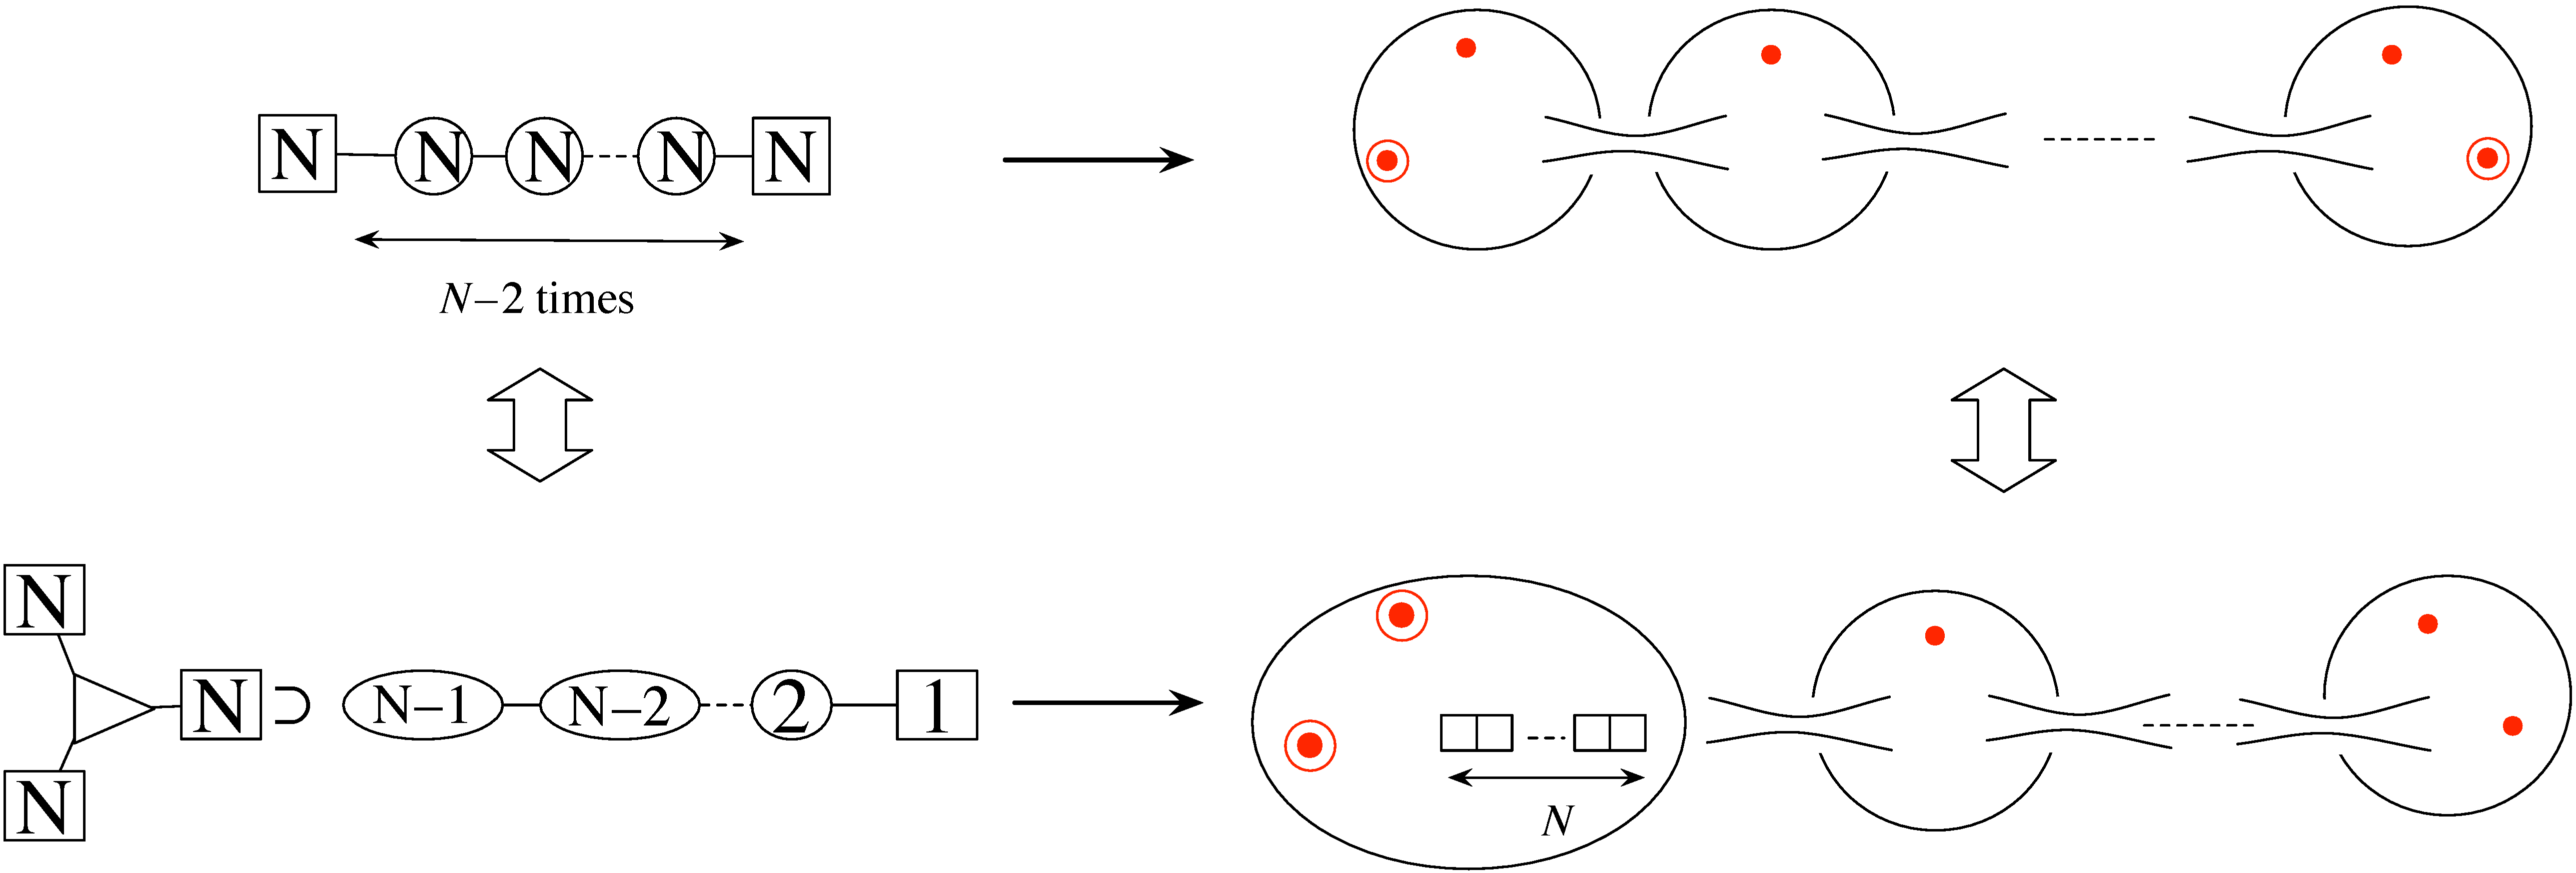
\includegraphics[width=\linewidth]{Tndual}}}
\]
\caption{产生 $T_N$ 理论的对偶。\label{fig:constructingTN}}
\end{figure}
现在可以愉快地摆弄一下穿孔了。例如，考虑规范群为 $\SU(N)^{N-2}$ 的规范理论，相邻群之间有双基本表示超多重态，首尾两个群还各有 $N$ 个额外的基本表示超多重态，见图 \ref{fig:constructingTN} 第一排。Seiberg-Witten 解很容易给出：它由 $\SU(N)$ 型理论的一个球面给出，带有两个完全穿孔和 $N-1$ 个简单穿孔。转到一个使这 $N-1$ 个简单穿孔全部退耦的对偶描述。应用第 \ref{sec:tame} 小节所学的退耦过程，得到规范群为
\begin{equation}
\SU(N-1)\times\SU(N-2)\times\cdots\SU(2),
\end{equation}
的箭图尾部，相邻两个群之间有双基本表示超多重态，最后的 $\SU(2)$ 还有一个二重态。第一个 $\SU(N-1)$ 规范化了类型为 $(1,1,\ldots,1)$ 的穿孔、即完全穿孔的味对称性 $\SU(N)$ 中的一个 $\SU(N-1)$ 子群。

\begin{figure}[h]
\[
\inc{Tn}
\]
\caption{$T_N$ 理论。\label{fig:TN}}
\end{figure}
通过这种方式，可以构造由带有三个完全穿孔的球面描述的理论。它称为 $T_N$ 理论，见图 \ref{fig:TN}。注意，$R_3=T_3$。由于有三个完全穿孔，味对称性至少为 $\SU(N)^3$。当 $N=3$ 时，前面已经看到，这一味对称性增强为 $E_6$。当 $N\ge4$ 时，原规范理论中不止有一个规范群。因此，不存在从 $\SU(N)\times\SU(N)$ 到其他群的增强。这与如下事实相符：当 $N\ge4$ 时，不存在一个包含 $\SU(N)^3$ 的群，使 $\SU(N)^2$ 增强为 $\SU(2N)$。将穿孔放在 $z=0,1,\infty$，可知 $\phi_k$ 具有形式
\begin{equation}
\phi_k=\frac{u_k^{(1)}+\cdots+u_k^{(k-2)}z^{k-3}}{z^{k-1}(z-1)^{k-1}}dz^k.
\end{equation}
因此，这一理论具有一个维数为 $3$ 的库仑支算符、两个维数为 $4$ 的库仑支算符，依此类推，直到 $N-2$ 个维数为 $N$ 的库仑支算符。

\begin{figure}[h]
\[
\begin{array}{c}
\inc{TnTn1}\\
\inc{TnTn2}
\end{array}
\]
\caption{相互耦合的 $T_N$ 理论副本的 S 对偶。\label{fig:TNTN}}
\end{figure}
现在，可以取两个 $T_N$ 理论的副本，并通过一个 $\SU(N)$ 规范多重态将它们耦合起来。在六维构造中，只是球面上有四个完全穿孔。因此，S 对偶结构与含有四个味的 $\SU(2)$ 理论完全相同，可以交换全部四个穿孔。事实上，$T_2$ 理论就是三基本表示超多重态 $Q_{ijk}$。

\subsubsection{$MN(E_7)$}\index{E7Theory@$E_7$ 理论|hyperpage}
\begin{figure}[h]
\[
\inc{E7dual}
\]
\caption{产生 $MN(E_7)$ 的对偶。\label{fig:constructingE7}}
\end{figure}
接下来，考虑图 \ref{fig:constructingE7} 中的对偶。最终得到一个三穿孔球面，带有两个完全穿孔和一个类型为 $(2,2)$ 的穿孔。在原规范理论中，有六个基本表示味耦合到 $\SU(4)$ 规范多重态，具有 $\SU(6)$ 味对称性。为了构造紫外曲线，将这六个味分为四个味和两个味，并应用图 \ref{fig:SUNtame} 第三排所示的规则。因此，三穿孔球面所代表的理论具有如下形式的味对称性 $F$：
\begin{equation}
\begin{array}{cccc}
F&\supset&\SU(6)&\times\SU(3)\\
\cup&&\cup\\
\SU(4)\times\SU(2)\times\SU(4)&\supset&\SU(4)\times\SU(2)\times\U(1)&\times\SU(3)
\end{array}.
\end{equation}

\begin{figure}[h]
\[
\inc{E7X}
\]
\caption{理论 $MN(E_7)$。\label{fig:E7}}
\end{figure}
幸而，这样的群 $F$ 唯一存在，即 $E_7$，见图 \ref{fig:E7}。当然，可以通过研究 $\phi_k(z)$ 来计算这一理论的库仑支算符数目。这里尝试另一种方法。原来的规范群是 $\SU(4)\times\SU(2)$，因此维数为 $2,3,4$ 的库仑支算符数目分别为 $2,1,1$。在对偶一侧，箭图尾部包含 $\SU(3)\times\SU(2)$，具有两个维数为 $2$ 的算符和一个维数为 $1$ 的算符。三穿孔球面所代表的理论应当补足差额。因此，它只有一个库仑支算符，维数为 $4$。这再次符合第 \ref{sec:rank-1SCFT} 小节宣称存在的一个秩为一的超共形理论的特征。它等价于 Minahan-Nemeschansky 理论 $MN(E_7)$。还可以像第 \ref{sec:AS} 小节末尾那样，检验流两点函数和希格斯支维数的一致性。
% [Tutor Note: p.159 原文 "two operators of dimension 2 and one operator of dimension 1" 中的 "dimension 1" 应为 "dimension 3"。判据：对偶一侧的箭图尾部为 $\SU(3)\times\SU(2)$，其库仑支算符的标度维数为 $\SU(3)$ 的 $2,3$ 与 $\SU(2)$ 的 $2$，即两个维数 $2$、一个维数 $3$；四维 $\cN{=}2$ 理论也不存在维数 $1$ 的库仑支算符。按此，三穿孔球面只需补足维数 $4$ 的那一个算符，与上下文的两组数目 $2,1,1$ 相符。正文照原文排版。]

\subsubsection{$MN(E_8)$}\index{E8Theory@$E_8$ 理论|hyperpage}
\begin{figure}[h]
\[
\inc{E8dual}
\]
\caption{产生 $MN(E_8)$ 理论的对偶。\label{fig:constructingE8}}
\end{figure}
现在，将它推广到 $E_8$ 对称性已经相当直接。进行图 \ref{fig:constructingE8} 所示的对偶变换。在对偶一侧，有一个三穿孔球面，带有一个完全穿孔、一个类型为 $(2,2,2)$ 的穿孔和一个类型为 $(3,3)$ 的穿孔。可知理论的味对称性 $F$ 应满足
\begin{equation}
\begin{array}{cccc}
F&\supset&\SU(5)&\times\SU(5)\\
\cup&&\cup\\
\SU(2)\times\SU(3)\times\SU(6)&\supset&\SU(2)\times\SU(3)\times\U(1)&\times\SU(5)
\end{array}.
\end{equation}
这与 Minahan-Nemeschansky 理论 $MN(E_8)$ 的结构吻合得很好，见图 \ref{fig:E8}。各种性质的检验留作读者练习。
\begin{figure}[h]
\[
\inc{E8X}
\]
\caption{$E_8$ 理论。\label{fig:E8}}
\end{figure}

\subsubsection{含有偶数个味的 $\SU(N)$ 理论的奇异极限}\label{sec:applicationL}\index{InfraredFreeTheory@红外自由理论|hyperpage}
最后，研究一个非共形的例子。考虑含有 $N_f=2n$ 个味的 $\SU(N)$ 理论，其中 $N>n$。曲线为
\begin{equation}
\frac{\Lambda^{N-n}\prod_{i=1}^n(x+\mu+\mu_i)}z
+\Lambda^{N-n}\prod_{i=1}^n(x+\mu+\tilde\mu_i)^nz
=x^N+u_2x^{N-2}+\cdots+u_N\label{Nn}
\end{equation}
微分为 $\lambda=xdz/z$。这里要求 $\sum_i\mu_i+\tilde\mu_i=0$，并将 $\U(1)$ 质量项单独记为 $\mu$。显然，当 $u_{N-n}=2\Lambda^{N-n}$ 时，$z\sim1$ 附近会发生一些事情。文献 \cite{Eguchi:1996vu} 最先考虑了这一点。正确的物理最初在文献 \cite{Gaiotto:2010jf} 中讨论。下面将看到，低能极限是一个与理论 $R_n$ 和 $X_{N-n+4}$ 耦合的红外自由 $\SU(2)$ 规范理论。

为了研究红外行为，令
\begin{equation}
u_{N-n,\text{old}}=2\Lambda^{N-n}+u_{N-n,\text{new}},\qquad z=1+\delta z
\end{equation}
并假定标度关系
\begin{equation}
\mu_i\sim\epsilon,\qquad
u_N\sim\epsilon^n,\quad u_{N-1}\sim\epsilon^{n-1},\quad\ldots,\quad u_{N-n+2}\sim\epsilon^2,\label{JJJ}
\end{equation}
以及
\begin{equation}
u_2\sim\epsilon'{}^2,\quad u_3\sim\epsilon'{}^3,\quad\ldots,\quad u_{N-n+2}\sim\epsilon'{}^{N-n+2}.
\end{equation}
于是，需要假定
\begin{equation}
\epsilon'{}^{N-n+2}\sim\epsilon^2.\label{ee}
\end{equation}
特别地，有
\begin{equation}
\epsilon\ll\epsilon'\ll1.
\end{equation}

在 $x\sim\epsilon$ 的区域中，可以将曲线 \eqref{Nn} 近似为
\begin{multline}
\frac{\Lambda^{N-n}\prod_{i=1}^n(x+\mu+\mu_i)}z
+\Lambda^{N-n}\prod_{i=1}^n(x+\mu+\tilde\mu_i)z\\
=(2\Lambda^{N-n}+u_{N-n})x^n+u_{N-n+2}x^{n-2}+\cdots+u_N
\end{multline}
并采用标度关系 \eqref{JJJ}。将它写成关于 $x$ 的 $n$ 次方程时，$x^n$ 项的系数为
\begin{equation}
\frac{\Lambda^{N-n}}z+\Lambda^{N-n}z-2\Lambda^{N-n}-u_{N-n}.\label{***}
\end{equation}
在极限 $\epsilon\to0$ 中，式 \eqref{***} 的两个零点在 $z=1$ 处碰撞。这正是第 \ref{sec:partII} 小节中，含有 $2n$ 个味的 $\SU(n)$ 理论在 $q\to1$ 极限下的情形。可以看到，得到的是与 $\SU(2)$ 规范群耦合的 $R_n$ 理论；算符 $u_{N-n+2}$ 现在被视为这一 $\SU(2)$ 的库仑支真空期望值。参数 $\mu_i$ 和 $\tilde\mu_i$ 现在是 $R_n$ 理论的 $\SU(2n)$ 对称性的质量参数。

在 $x\sim\epsilon'$ 的区域中，曲线 \eqref{Nn} 可以近似为
\begin{equation}
c\,\delta z^2=(x^{N-n}+u_2x^{N-n-2}+\cdots+\frac{u_{N-n+1}}x+\frac{u_{N-n+2}}{x^2}),
\end{equation}
其中微分 $\lambda=xd\delta z$，$c$ 是一个不重要的常数。在第 \ref{sec:ADAD} 小节已经遇到过它；它是描述含有两个味的 $\SU(N-n+1)$ 理论的 Argyres-Douglas 点的曲线。等价地，在第 \ref{sec:generalAD} 小节中将这一理论称为 $X_{N-n+4}$。

\begin{figure}[h]
\[
\inc{GSTX}
\]
\caption{含有 $N_f=2n$ 个味的 $\SU(N)$ 理论最奇异的点。\label{fig:EHIY}}
\end{figure}
总之，极限理论具有图 \ref{fig:EHIY} 所示的结构。具体而言，有一个弱耦合的 $\SU(2)$ 规范群，将 $x\sim\epsilon$ 的区域与 $x\sim\epsilon'$ 的区域连接起来：前者由 $\SU(n)$ 型六维理论的一个球面给出，代表 $R_n$ 理论；后者由 $\SU(2)$ 型六维理论的一个球面给出，代表理论 $X_{N-n+4}$。

在中间区域 $\epsilon'\gg x\gg\epsilon$ 中，曲线只是
\begin{equation}
\delta z^2\sim\frac{u_{N-n+2}}{x^2}
\end{equation}
微分为 $\lambda=\delta zdx\sim\sqrt{u_{N-n+2}}dx/x$。可见存在一个 $\SU(2)$ 规范群，且
\begin{equation}
a\sim\frac1{2\pi i}\oint\delta z\frac{dx}x\sim\sqrt{u_{N-n+2}}.
\end{equation}
于是，对偶坐标 $a_D$ 粗略地由下式给出：
\begin{equation}
a_D\sim\frac2{2\pi i}\int_{x\sim\epsilon'}^{x\sim\epsilon}\sqrt{u_{N-n+2}}\frac{dx}x
\sim\frac2{2\pi i}a\log\frac\epsilon{\epsilon'}.
\end{equation}
利用 $a\sim\epsilon$ 以及关系 \eqref{ee}，得到
\begin{equation}
a_D=\frac2{2\pi i}\frac{N-n}{N-n+2}a\log a+\cdots.
\end{equation}
回顾含有 $N_f$ 个味的 $\SU(2)$ 理论，其跑动由
\begin{equation}
a_D\sim\frac2{2\pi i}(4-N_f)a\log a+\cdots
\end{equation}
给出。因此，这一系统的有效味数为
\begin{equation}
N_f=\frac{5N-5n+8}{N-n+2}>4.
\end{equation}
现在 $\SU(2)$ 是红外自由的。注意，这正确地等于已经计算过的 $R_N$ 理论与 $X_{N-n+4}$ 理论的有效味数之和。确实，$R_N$ 理论的有效味数为 $3$，$X_{N-n+4}$ 理论的有效味数为 $2(N-n+1)/(N-n+2)$，分别见式 \eqref{k-of-su2} 和式 \eqref{GOO}。
\subsection{驯服穿孔与希格斯化}\label{sec:higgsing}\index{Higgsing@希格斯化|hyperpage}\index{NilpotentVev@幂零真空期望值|hyperpage}
\begin{figure}[h]
\[
\inc{partial-closing}
\]
\caption{穿孔类型的改变。\label{fig:partial-closing}}
\end{figure}

第 \ref{sec:tame} 小节以一种颇为临时性的方式，引入了紫外曲线上由杨图标记的穿孔。$\SU(4)$ 情形的例子展示在图 \ref{fig:SUNtame} 中。在本讲义最后一个小节里，我们希望稍微深入地研究杨图的意义。例如，应当如何理解图 \ref{fig:partial-closing} 中将完全穿孔变为简单穿孔、即类型为 $(3,1)$ 的穿孔的过程？本小节将始终以完全穿孔 $(1,1,1,1)$ 变为简单穿孔 $(3,1)$ 作为具体例子。推广到一般穿孔留作读者练习。本小节的内容基于作者与 Francesco Benini 在 2009 年至 2010 年间某时完成的一项未发表工作。

两者的 Seiberg-Witten 曲线都为
\begin{equation}
\lambda^4+\phi_2(z)\lambda^2+\phi_3(z)\lambda+\phi_4(z)=0.
\end{equation}
在两种情形中，$\phi_k(z)$ 都在 $z=0$ 处具有一个完全穿孔，在 $z=z_i$ 处具有五个简单穿孔。对于前者，$z=\infty$ 处原本是完全穿孔；对于后者，它是类型为 $(3,1,1)$ 的简单穿孔。

对于前者，场 $\phi_k(z)$ 为
\begin{equation}
\phi_k(z)=\frac{u_k^{(1)}+u_k^{(2)}z+u_k^{(3)}z^2+u_k^{(4)}z^3}{\prod_i^5(z-z_i)}\frac{dz^k}{z^{k-1}}.\label{former}
\end{equation}
对于后者，它们为
\begin{equation}
\begin{aligned}
\phi_2(z)&=\frac{u_2^{(1)}+u_2^{(2)}z+u_2^{(3)}z^2+u_2^{(4)}z^3}{\prod_i^5(z-z_i)}\frac{dz^2}z,\\
\phi_3(z)&=\frac{u_3^{(1)}+u_3^{(2)}z+u_3^{(3)}z^2}{\prod_i^5(z-z_i)}\frac{dz^3}{z^2},\\
\phi_4(z)&=\frac{u_4^{(1)}+u_4^{(2)}z}{\prod_i^5(z-z_i)}\frac{dz^4}{z^3}.
\end{aligned}\label{latter}
\end{equation}
这里，$u_k^{(i)}$ 是第 $i$ 个规范群的维数为 $k$ 的库仑支算符，根据极点结构确定它们的方法，已在式 \eqref{phifull} 附近说明。

显然，在式 \eqref{former} 中令 $u_4^{(3,4)}=u_3^{(4)}=0$，就得到式 \eqref{latter} 中的 $\phi_k(z)$。下面将解释，可以从第一个理论出发，将库仑支参数取在这一子空间上，然后移到希格斯支，从而实现第二个理论。

\begin{figure}[h]
\[
\inc{renaming-fields}
\]
\caption{为各场赋予新名称。\label{fig:renaming-fields}}
\end{figure}
为了便于分析希格斯支，为双基本表示引入新名称，见图 \ref{fig:renaming-fields}。将最右边的 $\SU(N)$ 味对称性命名为 $\SU(N)_0$，并从右向左将规范群命名为 $\SU(N)_{i=1,2,3,\ldots}$。为每个群引入一个辅助的 $N$ 维复空间 $V_i$。对于每一对相邻的 $\SU(N)_{i+1}\times\SU(N)_i$，有一个双基本表示超多重态 $(Q_b^a,\tilde Q_a^b)$，其中 $a=1,\ldots,N$ 和 $b=1,\ldots,N$ 分别是 $\SU(N)_{i+1}$ 与 $\SU(N)_i$ 的指标。将 $Q_b^a$ 视为线性映射 $A_i:V_i\to V_{i+1}$，将 $\tilde Q_a^b$ 视为反方向的映射 $B_i:V_{i+1}\to V_i$。注意，每一对 $(A_i,B_i)$ 都来自组成紫外曲线的若干三穿孔球面中的一个，如图所示。设总共有 $k$ 个三穿孔球面。

引入记号
\begin{equation}
M_i':=B_iA_i,\qquad\primeM_i:=A_iB_i.
\end{equation}
下面将反复使用显然的恒等式
\begin{equation}
\tr M_i'{}^n=\tr B_iA_i\cdots B_iA_i
=\tr A_iB_i\cdots A_iB_i=\tr{}\primeM_i{}^n.
\end{equation}

注意，$\tr M_i:=\tr M_i'=\tr\primeM_i$ 是第 $i$ 个 $\U(1)$ 味对称性的质量项，可以自然地与第 $i$ 个三穿孔球面的简单穿孔相联系。此外，还有另外两个规范不变组合，即
\begin{equation}
M_0'|_\text{traceless}:=M_0'-\frac1N\tr M_0,\qquad
\primeM_k|_\text{traceless}:=\primeM_k-\frac1N\tr M_k.
\end{equation}
$M_0'|_\text{traceless}$ 处于与最右侧球面在 $z=\infty$ 处的完全穿孔相联系的 $\SU(N)$ 味对称性的伴随表示中。类似地，$\primeM_k|_\text{traceless}$ 处于 $z=0$ 处穿孔的 $\SU(N)$ 味对称性的伴随表示中。

现在，我们希望通过给伴随表示场 $M_0'|_\text{traceless}$ 赋予非零真空期望值，对 $z=\infty$ 处的穿孔作局部修改。其他规范不变组合 $\tr M_i$（$i=1,\ldots,k$）和 $\primeM_k|_\text{traceless}$ “局域”在其他穿孔处。因此选择让它们保持为零。

来自 $\SU(N)_i$ 规范多重态中伴随表示标量的 F 项关系为
\begin{equation}
M_{i+1}'|_\text{traceless}={}\primeM_i|_\text{traceless}.
\end{equation}
由于施加了条件 $\tr M_i=0$，可以去掉取无迹部分的条件，直接写成
\begin{equation}
M_{i+1}'={}\primeM_i.
\end{equation}
于是，对任意 $n$，有如下关系：
\begin{equation}
\tr M_0'{}^n=\tr\primeM_0{}^n=\tr M_1'{}^n=\tr\primeM_1{}^n
=\cdots=\tr M_k'{}^n=\tr\primeM_k{}^n=0.
\end{equation}

这意味着，按 $\SU(N)$ 味对称性的伴随表示变换的规范不变组合 $M_0'$ 是一个幂零矩阵。可以通过复化的 $\SU(N)$ 旋转，将它化为 Jordan 标准形：
\begin{equation}
M_0'=J_{t_1}\oplus J_{t_2}\oplus\cdots,\qquad\sum_it_i=N\label{nilpotent-vev}
\end{equation}
其中 $J_t$ 是大小为 $t$ 的 Jordan 块，
\begin{equation}
J_t=\underbrace{\begin{pmatrix}
0&1\\
&0&1\\
&&0&1\\
&&&\ddots&\ddots\\
&&&&0
\end{pmatrix}}_t.
\end{equation}

再次得到了 $N$ 的一个分拆 $(t_i)$。下面将论证，这一分拆 $(t_i)$ 恰好就是第 \ref{sec:tame} 小节中用来标记穿孔的杨图。为了研究真空期望值 \eqref{nilpotent-vev} 的影响，需要找到一组满足 F 项和 D 项关系的超多重态场 $(A_i,B_i)$ 的取值。

\begin{figure}[h]
\[
\inc{more-notation}
\]
\caption{矩阵的图示记号。\label{fig:more-notation}}
\end{figure}
为了写出这样一组取值，再引入一种图示记号很有用，见图 \ref{fig:more-notation}。$N$ 维向量空间 $V$ 具有 $N$ 个基向量，用一列 $N$ 个点来表示它们。从 $V$ 到 $V'$、矩阵元为 $0$ 或 $1$ 的矩阵，可以用一组箭头表示：当且仅当矩阵的第 $(a,b)$ 元为 $1$ 时，从 $V$ 的第 $a$ 个点向 $V'$ 的第 $b$ 个点画一条箭头。图 \ref{fig:more-notation} 中间表示了大小为 $4$ 的 Jordan 块 $J_4$。同一图最右侧的图示表示投影到最后两个基向量的投影算符。

\begin{figure}[h]
\[
\inc{Higgsing}
\]
\caption{希格斯支上的一个特定点。\label{fig:higgsing}}
\end{figure}
为明确起见，令 $N=4$，并给 $M_0'$ 赋予类型为 $(3,1)$ 的幂零真空期望值，即由 $J_3\oplus J_1$ 给出。图 \ref{fig:higgsing} 给出 F 项关系的一个解。从中可以看到，此时未破缺的规范群为 $\SU(4)\times\SU(4)\times\SU(3)\times\SU(2)$。

一般而言，可以如下构造 F 项关系的解。假设希望令 $M_0'=X$，其中 $X$ 处于 Jordan 标准形。将向量空间作等同 $V_0=V_1=V_2=\cdots$。引入记号 $W_i=\Im X^i$，并将到 $W_i$ 的投影算符记为 $P_{W_i}$。然后令
\begin{equation}
A_0=X,\quad A_1=XP_{W_1},\quad A_2=XP_{W_2},\ldots
\end{equation}
并取
\begin{equation}
B_0=P_{W_1},\quad B_1=P_{W_2},\quad B_2=P_{W_3},\ldots.
\end{equation}
显然，剩余规范群具有形式
\begin{equation}
\cdots\times\SU(N_3)\times\SU(N_2)\times\SU(N_1)
\end{equation}
其中
\begin{equation}
N_i=N-\dim W_i=N-\rank X^i.
\end{equation}
定义 $s_i=N_i-N_{i-1}$。简短的组合计算表明：当 $X$ 的类型由一个从左数第 $i$ 列高度为 $t_i$ 的杨图描述时，序列 $(s_1,s_2,\ldots)$ 中的 $s_i$ 就是从下往上数第 $i$ 行的宽度。这正是第 \ref{sec:tame} 小节已经引入的规范群规则。现在来确定所得理论的无质量物质内容。

一种间接但迅速的确定物质内容的方法如下。我们从一个不含任何参数的超共形理论出发。希格斯化之后，唯一具有质量量纲的参数是超多重态场的真空期望值。根据第 \ref{sec:hypergeneral} 小节讨论过的拉格朗日量中超多重态部分与矢量多重态部分的一般退耦性质，希格斯化之后的低能理论中不能出现任何质量项或动力学能标。因此，所得理论也是超共形的。已经确定了 $N_i$，而且只能存在双基本表示场或基本表示场。这表明，$\SU(N_i)$ 应当恰好具有
\begin{equation}
n_i=2N_i-N_{i+1}-N_{i-1}\label{additional-funds}
\end{equation}
个额外的基本表示超多重态。

\begin{figure}[h]
\[
\inc{mass-term}
\]
\caption{为标量场产生的质量项。\label{fig:mass-term}}
\end{figure}
当然，这一结果也可以通过直接计算系统中各个场的质量项得到。注意，原来存在 $\cN{=}1$ 超势 $\tr A_i\Phi_iB_i$ 和 $\tr B_i\Phi_{i+1}A_i$，其中 $\Phi_i$ 是 $\SU(N)_i$ 矢量多重态中的伴随表示标量。由于给 $A_i$ 与 $B_i$ 的某些分量赋予了真空期望值，三点耦合会使超多重态标量与矢量多重态标量的某些分量配对。图 \ref{fig:mass-term} 展示了一个例子。其中，用向左下方的箭头表示的 $A_1$ 的真空期望值，使对应于 $V_2$ 的规范群的矢量多重态标量的一个分量与 $B_1$ 的一个分量之间产生质量项。

\begin{figure}[h]
\[
\inc{remaining-fields}
\]
\caption{希格斯化后剩下的场。\label{fig:remaining-fields}}
\end{figure}
可以看到，始终有一个 $\SU(N_{i+1})\times\SU(N_i)$ 的双基本表示保持无质量。但是，仔细分析质量项后会发现，有时还有更多带荷超多重态保持无质量。例如，如图 \ref{fig:remaining-fields} 所示，$V_3$ 与 $V_2$ 之间的整个双基本表示都保持无质量。在 $V_2$ 处，$\SU(4)$ 破缺到 $\SU(3)$。因此，从 $V_3$ 处未破缺的 $\SU(4)$ 的观点看，存在一个 $\SU(4)\times\SU(3)$ 双基本表示，以及一个 $\SU(4)$ 基本表示。将这一分析推广，就可以看出 $\SU(N_i)$ 的额外基本表示超多重态数目由式 \eqref{additional-funds} 给出。

\begin{figure}[h]
\[
\inc{flavor-telekinesis}
\]
\caption{味对称性的分配。\label{fig:flavor-telekinesis}}
\end{figure}

第 \ref{sec:tame} 小节曾说，$z=\infty$ 处的穿孔承载了与连接到 $\SU(N_i)$ 的额外 $n_i$ 个基本表示超多重态相关的全部味对称性。这听起来多少有些违背直觉，因为味对称性 $\SU(n_i)$ 看上去更应与第 $i$ 个节点相联系。现在可以理解这里起作用的物理机制了。为明确起见，再取类型为 $(3,1)$ 的穿孔，见图 \ref{fig:flavor-telekinesis}。根据我们的规则，真空期望值 $X=M_0'$ 为 $X=J_3\oplus J_1$；它在作用于三个基向量的 $\U(1)$ 旋转下不变，这三个基向量用图中的黑点表示。如果不伴随规范旋转，这一对称性并不保持希格斯真空期望值 $\vev{A_i}$ 和 $\vev{B_i}$ 不变。为了使对称性与希格斯真空期望值相容，需要同时旋转其他所有基向量：它们通过代表 $A_i$ 和 $B_i$ 的箭头，与原来的黑点相连接。

可以看到，希格斯真空期望值将旋转 $V_0$ 的三个基向量的 $\U(1)$ 味对称性，与旋转 $V_3$ 最后一个基向量的 $\U(1)$ 味对称性对应起来。希格斯化之后，后一个 $\U(1)$ 对称性恰好就是 $V_3$ 处 $\SU(4)$ 的额外一个基本表示超多重态所承载的味对称性，图中用实心三角形表示。这一分析可以推广到任意类型的穿孔。

总之，我们找到了对第 \ref{sec:tame} 小节引入的穿孔的一种新解释。这样的穿孔始终可以从完全穿孔得到：先将库仑支真空期望值选在适当的子空间上，再给超多重态组合 $M_0'$ 赋予幂零真空期望值；$M_0'$ 按与完全穿孔相联系的味 $\SU(N)$ 的伴随表示变换。赋予 $M_0'$ 的真空期望值，使某些 $i>0$ 的其他超多重态场 $A_i$、$B_i$ 获得非零真空期望值，从而将原规范群 $\cdots\times\SU(N)\times\SU(N)\times\SU(N)$ 破缺为 $\cdots\times\SU(N_3)\times\SU(N_2)\times\SU(N_1)$。

\section{结论与后续方向}\label{sec:conclusions}

在本讲义中，我们首先讨论了 $\cN{=}2$ 超对称规范理论的拉格朗日量，然后研究了含有不同味数的 $\SU(2)$ 规范理论的库仑支和希格斯支。在这一过程中，Seiberg-Witten 曲线和紫外曲线这两个相关概念发挥了非常重要的作用。随后，我们分析了精细调节库仑支真空期望值或恰好边缘耦合参数时会发生什么。有时，这一极限由一个对偶的弱耦合规范理论描述，含有四个味的 $\SU(2)$ 理论便是如此。然而，在大多数情况下，我们看到最终得到的是新的超共形场论，属于 Argyres-Douglas 型或 Gaiotto 型。

例如，我们在第 \ref{sec:rank-1SCFT} 小节中见到了理论 $AD_{N_f=1,2,3}(\SU(2))$ 和 $MN(E_{6,7,8})$，在第 \ref{sec:generalAD} 小节中见到了理论 $X_N$ 和 $Y_N$，在第 \ref{sec:partII} 小节中见到了 $R_N$，在第 \ref{sec:application} 小节中见到了 $T_N$。越来越多的 $\cN{=}2$ 超共形理论正在被发现，例如见文献 \cite{Cecotti:2010fi,Cecotti:2012jx,Cecotti:2013lda}。这意味着，要充分理解 $\cN{=}2$ 超对称系统之间的相互关系，就不能只关注由矢量多重态和超多重态组成的 $\cN{=}2$ 理论。

本讲义所涉及的主题，只是 $\cN{=}2$ 动力学研究这座巨大冰山的一角，还有许多进一步的研究方向。下面列举其中一些。\footnote{作者在这里并未力求穷尽和全面，只引用了少数近期文献。如有人提出请求，作者很乐意补充更多引文。} 首先，可以把一个 $\cN{=}2$ 理论放在非平凡流形上：
% [Tutor Note: p.169 原文 "a nontrival manifold" 中 "nontrival" 应为 "nontrivial"，系拼写笔误；译文按本意作“非平凡流形”。]
\begin{itemize}
\item 利用拓扑扭曲\index{TopologicalTwist@拓扑扭曲|hyperpage}，可以把它放在任意流形上 \cite{Witten:1988ze}。当流形紧致时，配分函数等价于数学家所说的 Donaldson 不变量。将 Seiberg-Witten 解应用于纯 $\SU(2)$ 理论，Witten 引入了一个新的数学不变量，如今称为 Seiberg-Witten 不变量\index{SeibergWittenInvariant@Seiberg-Witten 不变量|hyperpage} \cite{Witten:1994cg}；二十年前，它给四维微分几何带来了一场革命。
\item 可以把它放在 $S^1$ 上。此时理论在有效意义上是三维的。正如文献 \cite{Seiberg:1996nz} 首次分析的那样，作为三维理论的库仑支，自然地是在四维理论库仑支之上的一个纤维化。三维库仑支是超凯勒的，并具有有限自由度经典可积系统的结构。这一可积系统最初在文献 \cite{Donagi:1995cf} 中引入。关于现代发展，例如见文献 \cite{Gaiotto:2008cd}。
\item 可以把它放在所谓的 $\Omega$ 背景上。非常粗略地说，这涉及使 $\bR^4$ 上的整个欧氏系统绕原点作强制旋转。时空在有效意义上是紧致的，因而可以定义配分函数，通常称为 Nekrasov 配分函数。关于近期的全面讨论，例如见文献 \cite{Nekrasov:2012xe}。文献 \cite{Nekrasov:2009rc} 发现，在某种极限情形下，它给出一个量子化可积系统，即 Donagi-Witten 可积系统的量子化版本。
\item 可以把它放在圆的或形变的 $S^4$ 上。时空是紧致的，配分函数可以精确计算，例如见文献 \cite{Pestun:2007rz,Hama:2012bg,Nosaka:2013cpa}。还已知该配分函数与紫外曲线上的二维共形场论有关，例如见文献 \cite{Alday:2009aq,Wyllard:2009hg}。
\item 可以把它放在 $S^1\times S^3$ 上。配分函数称为超共形指标\index{SuperconformalIndex@超共形指标|hyperpage}，并给出紫外曲线上的二维拓扑场论。它还与多种重要的正交多项式有深刻联系，例如见文献 \cite{Gadde:2011uv,Gaiotto:2012xa}。
\item 也可以考虑其他背景。关于 $S^2\times S^1\times\bR$，见文献 \cite{Luo:2013nxa}。文献 \cite{Closset:2013sxa} 研究了 $T^2\times S^2$ 上的 $\cN{=}1$ 理论，当然也可以在那里类似地考虑 $\cN{=}2$ 系统。
\end{itemize}
其次，可以研究这些理论的动力学激发和从外部引入的算符：
\begin{itemize}
\item 我们已经看到，如何从六维构造读出饱和 BPS 界的粒子种类数。这个数是整数，因此通常不能改变，但它确实会在库仑支上的某些位置发生跳跃。这称为跨墙\index{WallCrossing@跨墙|hyperpage}，是一个受到深入研究的领域，例如见文献 \cite{Gaiotto:2009hg}。所得的谱通常可以用一种称为 BPS 箭图\index{BPSQuiver@BPS 箭图|hyperpage}的图来概括。这一观点最初在文献 \cite{Denef:2002ru} 中的 $\cN{=}2$ 超引力背景下引入。关于较新的发展，例如见文献 \cite{Denef:2007vg,Cecotti:2011rv,Manschot:2012rx}。
\item 不引入动力学粒子，也可以引入外部对象的世界线。它们称为线算符\index{LineOperator@线算符|hyperpage}。例如见文献 \cite{Drukker:2009tz,Gaiotto:2010be}。
\item 一旦允许引入外部线算符，就没有理由不引入更高维的外部对象。当它们具有两个时空维度时，称为面算符\index{SurfaceOperator@面算符|hyperpage}。Seiberg-Witten 曲线可以内禀地定义为一个面算符的红外模空间 \cite{Gaiotto:2009fs}。另一篇值得研读的近期有趣论文是文献 \cite{Gaiotto:2013sma}。
\item 进而可以考虑具有三个时空维度的对象。这就是外部畴壁\index{DomainWall@畴壁|hyperpage}。关于近期的研究，例如见文献 \cite{Dimofte:2013lba}。
\end{itemize}
关于这些主题，综述 \cite{MooreReview} 是极好的资料来源，尽管该综述本身是面向数学家的。

第三，本讲义所描述的方法还不足以求解任意的 $\cN{=}2$ 规范理论。许多四维 $\cN{=}2$ 理论确实来自六维 $\cN{=}(2,0)$ 理论，但目前也有许多理论并非如此。因此，还应该研究其他方法。
\begin{itemize}
\item 六维构造本身还需要进一步发展。关于驯服穿孔的进一步讨论，例如见文献 \cite{Chacaltana:2010ks,Chacaltana:2012ch,Chacaltana:2013oka}；关于野性穿孔，更多内容见文献 \cite{Xie:2012hs,Xie:2013jc}。
\item 四维 $\cN{=}2$ 理论的六维构造，总能提升为非紧致 Calabi-Yau 流形上的 IIB 型弦论，该流形是紫外曲线之上的一个纤维化。即便这个非紧致 Calabi-Yau 流形不是曲线之上的纤维化，其上的 IIB 型弦论也常常实现一个四维 $\cN{=}2$ 场论，这为求解 $\cN{=}2$ 系统提供了另一种途径，例如见文献 \cite{Tachikawa:2011yr,Cecotti:2012sf}。
\item 对于一般规范群 $G$，$\cN{=}2^*$ 理论，即通过伴随超多重态的质量项使 $\cN{=}4$ 超杨--米尔斯理论发生形变而得到的理论，早已得到求解 \cite{D'Hoker:1999ft}。有些令人惊讶的是，当 $G\neq\SU(N)$ 时，目前还不知道这些解的明确弦论或 M 理论构造。这清楚地表明，我们目前的理解还多么初步。
\end{itemize}

第四，$\cN{=}2$ 理论有许多性质为所有已知例子所满足，但目前还没有办法推导它们。设计研究这些性质的新方法，应当会富有成效。下面列出这一方向上的几个问题。
\begin{itemize}
\item $\cN{=}2$ 规范理论库仑支上的手征算符显然总是自由生成的。例如，在 $\SU(N)$ 规范理论中，它们由 $\tr\phi^k$（$k=2,\ldots,N$）生成，这些算符之间没有非平凡关系。从已有例子来看，由六维构造得到的所有非拉格朗日理论仍满足这一性质：库仑支算符是自由生成的。作者猜想，这实际上是一条适用于每个 $\cN{=}2$ 超对称系统的定理。
\item 文献 \cite{Buican:2013ica} 论证了，在两个 $\cN{=}2$ 超共形场论之间的重整化群流中，中心荷 $a$ 的变化存在一个非零下界。能否更严格地推导这一事实？
% [Tutor Note: p.171 原文 "Is there are more rigorous derivation of this fact?" 中 "there are" 应为 "there a"（即 "Is there a more rigorous derivation …"），系笔误；译文按本意译出。]
\item 能否刻画整个 $\cN{=}2$ 理论谱系本身？作一个类比，考虑 $\SU(2)$ 的所有表示。如果只允许直和，就需要所有不可约表示，才能构造所有可能的表示。如果还允许张量积以及取出一个不可约直和分量，那么只需要二维不可约表示，就能生成所有其他表示。

对于 $\cN{=}2$ 理论，也可以提出类似的问题。如果只允许弱规范化，需要哪些广义物质内容，即超多重态和其他“不可约”的强耦合理论，才能生成所有 $\cN{=}2$ 理论？如果还允许强耦合极限、S 对偶以及分解为组成部分，那么需要多少？通过六维、弦论或 M 理论构造，能够得到这些理论的多大“百分比”？

在某种技术意义下完备的 $\cN{=}2$ 理论，已在文献 \cite{Cecotti:2011rv} 中得到分类；$\cN{=}2$ 弱耦合规范理论，已在文献 \cite{Bhardwaj:2013qia} 中得到分类。不过，这只是进入所有可能的 $\cN{=}2$ 理论所构成的广阔空间的两个小小步骤。本讲义中见到的理论汇总于附录 \ref{sec:zoo}。
\end{itemize}

最后，作者想强调，即便是下列看起来如此简单的规范理论：
\begin{itemize}
\item 带有一个三指标反对称张量表示超多重态的 $\cN{=}2$ 超对称 $\SU(7)$ 规范理论，或
\item 带有一个有质量的三基本表示完整超多重态 $(Q_{aiu},\tilde Q^{aiu})$ 的 $\cN{=}2$ 超对称 $\SU(2)^3$ 规范理论，
\end{itemize}
也还没有得到求解。对于第一个求出这两个理论中任意一个的解的人，作者很乐意在柏校区的寿司店请他吃一顿晚餐。如文献 \cite{Bhardwaj:2013qia} 所列，还有许多其他 $\cN{=}2$ 规范理论没有已知的解。因此，这个领域仍应被看作大有可为。

希望读到这里的读者，至少已经具备了一定的基础，可以着手研读这些以及其他关于 $\cN{=}2$ 超对称理论的近期论文。如果他们继续学习，并为拓展研究前沿作出贡献，作者将感到十分欣慰。

\appendix
\section{预势与瞬子计算}\label{sec:instcount}
在第 \ref{sec:purecurve} 小节中，我们学会了如何借助 Seiberg-Witten 曲线求出纯 $\SU(2)$ 理论的 $a$ 和 $a_D$。将 $a_D$ 积分两次，便可以具体确定预势 $F(a)$。在本附录中，我们先进行这一计算，然后非常简要地解释，如何通过微观路径积分计算得到同一个预势。

\subsection{由曲线求预势}\index{Prepotential@预势|hyperpage}\index{RenormalizationGroupRelation@重整化群关系|hyperpage}\index{RiemannReciprocityLaw@Riemann 互反律|hyperpage}
纯 $\SU(2)$ 理论的曲线已在式 \eqref{curve_pure} 中给出，这里再次写出：
\begin{equation}
\Lambda^2 z+\frac{\Lambda^2}z=x^2-u,
\end{equation}
其微分为 $\lambda=xdz/z$。$a$ 和 $a_D$ 由下式确定：
\begin{equation}
a=\frac{1}{2\pi i}\oint_A\lambda,\qquad
a_D=\frac{1}{2\pi i}\oint_B\lambda.\label{aad}
\end{equation}
由此，应当确定满足 $a_D=\partial F/\partial a$ 的 $F(a)$。低能耦合为 $\tau(a)=\partial a_D/\partial a$。在式 \eqref{tauexpansion} 中，我们得到了 $\tau(a)$ 的弱耦合展开形式。积分两次，便看到 $F(a)$ 具有展开
\begin{equation}
2\pi iF(a)=-4a^2\log\frac{a}{\Lambda}+\sum_{k=1}^\infty d_k\frac{\Lambda^{4k}}{a^{4k-2}}\label{Fweak}
\end{equation}
其中 $d_k$ 是纯数。下面遵循文献 \cite{Chan:1999gj}，明确求出它们。

为此，使用所谓的重整化群关系
\begin{equation}
2\pi i\Lambda\frac{\partial}{\partial\Lambda}F(a,\Lambda)=4u\label{matone}
\end{equation}
它最初在文献 \cite{Matone:1995rx} 中推导出来。这一关系可以用多种方法证明。一种直接的方法是注意到，由式 \eqref{lambdaSU2pure} 可得
\begin{equation}
2\pi i\Lambda\frac{\partial}{\partial\Lambda}=4\frac{\partial}{\partial\tau_{UV}}
\end{equation}
这里保持紫外调节参数 $\Lambda_{UV}$ 不变。回顾紫外能标处的预势为 $F(\phi)=(\tau_{UV}/2)\tr\phi^2$，见第 \ref{sec:lel} 小节末尾。于是，关系 \eqref{matone} 只是下述陈述：
\begin{equation}
\frac{\partial}{\partial\tau_{UV}}\vev{F}=\frac12\vev{\tr\phi^2}=u.
\end{equation}

也可以选择从式 \eqref{aad} 出发，以纯数学方式证明关系 \eqref{matone}。从显然的关系开始：
\begin{equation}
(\Lambda\frac{\partial}{\partial\Lambda}+a\frac{\partial}{\partial a})F=2F.
\end{equation}
利用它，得到
\begin{align}
\frac{\partial}{\partial u}\Lambda\frac{\partial}{\partial\Lambda}F
&=\frac{\partial}{\partial u}(2F-a\frac{\partial}{\partial a}F)
=a\frac{\partial a_D}{\partial u}-\frac{\partial a}{\partial u}a_D\\
&=\frac1{(2\pi i)^2}\left(\oint_A\lambda\oint_B\frac{\partial}{\partial u}\lambda-\oint_A\lambda\oint_B\frac{\partial}{\partial u}\lambda\right).
\end{align}
这里，$\lambda=xdz/z$ 是第二类微分（即留数为零的亚纯微分），而 $\partial\lambda/\partial u=-dz/(2xz)$ 是第一类微分（即全纯微分）。因此，可以利用 Riemann 互反律来计算，例如见文献 \cite{GH} 第 2.3 节。具体地说，$\lambda$ 的二阶极点位于 $z=0$ 和 $\infty$。在这两点处，$w:=1/x$ 都是良好的局部坐标，并且有展开
\begin{equation}
\lambda=x\frac{dz}z=-2\frac{dw}{w^2}+\cdots,\qquad
\frac{\partial}{\partial u}\lambda=-\frac{dz}{2xz}=dw+\cdots.
\end{equation}
所以有
\begin{equation}
\frac{\partial}{\partial u}\Lambda\frac{\partial}{\partial\Lambda}F=\frac4{2\pi i},
\end{equation}
从而证明了式 \eqref{matone}。

现在回到式 \eqref{Fweak} 中系数 $d_k$ 的计算。令 $u=\underline a^2$，则
\begin{align}
a(\underline a)&=\frac1{2\pi i}\oint_A\lambda=\frac1{2\pi i}\oint_A(\sum_{l=0}^\infty
(z+\frac1z)^l\frac{(-1)^l(2l)!}{(1-2l)(l!)^2 2^{2l}}
\frac{\Lambda^{2l}}{\underline a^{2l-1}})\frac{dz}z\\
&=\underline a\sum_{k=0}^\infty\frac{\Lambda^{4k}}{\underline a^{4k}}\frac1{(1-4k)2^{4k}}\frac{(4k)!}{(2k)!k!k!}.\label{113}
\end{align}
现在，将展开 \eqref{Fweak} 代入关系 \eqref{matone}，得到
\begin{equation}
a^2(1+\sum_{k=1}^\infty k d_k\frac{\Lambda^{4k}}{a^{4k}})=\underline a^2.\label{114}
\end{equation}
关系 \eqref{113} 和 \eqref{114} 合在一起，足以递归确定 $d_k$。最前面的几项是
\begin{equation}
d_1=\frac12,\quad d_2=\frac5{64},\quad d_3=\frac3{64},\quad d_4=\frac{1469}{32768},\quad\ldots.\label{results-from-curve}
\end{equation}

\subsection{由瞬子计算求预势}
这里从更微观的观点，介绍同一预势的另一种计算。这一计算可以完全用纯 $\SU(2)$ 规范理论的路径积分来表述 \cite{Nekrasov:2002qd}。利用一个密切相关的五维场论，基本相同的计算可以用更物理的方式来表述。我们在这里采用后一种方法。这里的介绍将非常简略；更多细节请读者参阅文献 \cite{TachikawaInstantonReview}。

\subsubsection{$\Omega$ 背景}\index{OmegaBackground@$\Omega$ 背景|hyperpage}\index{NekrasovPartitionFunction@Nekrasov 配分函数|hyperpage}
首先利用这样一个事实：给定一个四维 $\cN{=}2$ 超对称规范理论，其规范群为 $G$，超多重态属于 $G$ 的表示 $R$，也可以考虑一个五维超对称规范理论，具有相同的规范群 $G$，超多重态属于相同的表示 $R$；将该理论紧致化在半径为 $\beta$ 的 $S^1$ 上，再取零半径极限 $\beta\to0$，就恢复原来的四维理论。

\begin{figure}[h]
\[
\inc{omega}
\]
\caption{五维 $\Omega$ 背景的示意图。\label{fig:omega}}
\end{figure}
我们在所谓的 $\Omega$ 背景上考虑这个五维理论，该背景按如下方式得到。首先，将 $\bR^5$ 看作 $\bC^2\times\bR$，坐标为 $(z_1,z_2,x_5)$，其中 $z_{1,2}$ 为复数，$x_5$ 为实数。然后作等同
\begin{equation}
(z_1,z_2,x_5)\sim(z_1e^{i\beta\epsilon_1},z_2e^{i\beta\epsilon_2},x_5+\beta).\label{omegaident}
\end{equation}
为了保持超对称性，必须在这一等同 \eqref{omegaident} 的同时进行 $\SU(2)_R$ 旋转
\begin{equation}
\diag(e^{i\beta(\epsilon_1+\epsilon_2)/2},e^{-i\beta(\epsilon_1+\epsilon_2)/2})\in\SU(2)_R.
\end{equation}
在作等同 \eqref{omegaident} 时，也可以选择进行规范旋转
\begin{equation}
e^{i\beta\vec a}\in G
\end{equation}
其中 $\vec a$ 是 $G$ 的李代数中的一个元素。图 \ref{fig:omega} 给出了该系统的示意图。

这个时空的第五方向为 $\beta$，并伴随着 $\bR^4$ 一侧转过角度 $\beta\epsilon_{1,2}$。当把 $x_5$ 看作时间方向时，系统被迫旋转，远离 $\bC^2$ 原点的任何激发都要耗费很大的能量。这使系统在有效意义上具有有限体积，大小为 $\sim1/(\epsilon_1\epsilon_2)$。因此，系统具有有限的配分函数 $Z(\epsilon_{1,2},\tau_{UV};\vec a)$，其对数表现为
\begin{equation}
\log Z(\epsilon_{1,2},\tau_{UV};\vec a)=\frac1{\epsilon_1\epsilon_2}\cF(\tau_{UV};\vec a)+\text{关于 $\epsilon_{1,2}$ 奇异性较弱的项},
\end{equation}
其中 $\cF$ 是系统单位体积的自由能。这里用五维耦合常数 $g_{UV5}$ 定义 $\tau_{UV}$；$g_{UV5}$ 的定义使规范动能项具有形式
\begin{equation}
\int dx_5\int d^4x\frac1{2g_{UV5}{}^2}\tr F_{\mu\nu}F_{\mu\nu}.\label{5dgaugekin}
\end{equation}
先对 $x_5$ 积分，产生一个因子 $\beta$，于是得到
\begin{equation}
\tau_{UV}=\beta\frac{4\pi i}{g_{UV5}{}^2}.
\end{equation}

一个基本事实是，这个自由能 $\cF$ 等于预势：
\begin{equation}
2\pi iF(\tau_{UV};\vec a)=\cF(\tau_{UV};\vec a)=\lim_{\epsilon_{1,2}\to0}\epsilon_1\epsilon_2\log Z(\tau_{UV};\vec a).\label{main-instanton-formula}
\end{equation}
取一个受控的极限 $\beta\to0$，便可以提取纯四维理论的预势。这一适用于任意 $\cN{=}2$ 理论的普遍事实，可以用多种方法推导，见文献 \cite{Nekrasov:2002qd} 或文献 \cite{Tachikawa:2004ur} 的附录。

\subsubsection{约化为超对称量子力学}\index{InstantonModuliSpace@瞬子模空间|hyperpage}\index{SupersymmetricQuantumMechanics@超对称量子力学|hyperpage}
这种重新表述听起来或许繁琐，但其好处在于，预势的计算如今归结为 $\Omega$ 背景 \eqref{omegaident} 中系统的配分函数 $Z$ 的计算。将系统约化为超对称量子力学，便可以用与第 \ref{sec:box} 小节中分析盒子内的纯 $\cN{=}1$ 规范理论大致相同的方法完成计算。注意，这里将额外维度 $x^5$ 看作时间方向 $t$。

总配分函数 $Z$ 是微扰部分 $Z_\text{pert}$ 与非微扰部分 $Z_\text{non-pert}$ 的乘积。第一部分只再现式 \eqref{Fweak} 中领头的对数项，其再现方式本身颇为有趣，但这里不再介绍。相反，下面集中讨论非微扰部分 $Z_\text{non-pert}$。计算这一部分时，可以像第 \ref{sec:box} 小节那样，限制在每个拓扑扇区中的最低能态。从式 \eqref{5dgaugekin} 可以看出，一个规范场构型的能量包含贡献
\begin{equation}
\int d^4x\frac1{2g_{UV5}{}^2}\tr F_{\mu\nu}F_{\mu\nu},\label{5dprefactor}
\end{equation}
正如式 \eqref{bound} 所示，其下界为 $8\pi^2|k|/g_{UV5}{}^2$，其中 $k$ 为瞬子数。

因此，唯一对 $Z$ 的计算有贡献的经典场构型，是在每个等时面 $t=\text{常数}$ 上都具有瞬子构型的场构型。瞬子数 $k$ 是整数，所以沿时间演化时不能改变。然而，固定 $k$ 的瞬子构成一个连续族，因此瞬子的形状可以变化。用 $M_k$ 表示这一连续族的参数空间，称为瞬子模空间。给定一点 $p\in M_k$，就有一个瞬子解 $F_{\mu\nu}(x_{1,2,3,4};p)$，其中 $\mu,\nu=1,2,3,4$。随时间 $t=x_5$ 变化，瞬子的形状也发生变化。换言之，存在 $M_k$ 中的一条路径 $p(t)$。此时，五维作用量 \eqref{5dgaugekin} 近似变为
\begin{equation}
\int dt\int d^4x\frac1{2g_{UV5}{}^2}\tr F_{\mu\nu}F_{\mu\nu}
=\int dt(\frac{8\pi^2}{2g_{UV5}{}^2}+G_{IJ}(p)\partial_t p^I(t)\partial_t p^J(t))\label{sqm}
\end{equation}
其中，右侧的第一项和第二项分别来自左侧时空指标 $\mu,\nu$ 中不含 $5$ 和含有 $5$ 的项。这里，指标 $I=1,\ldots,\dim M_k$ 对应于 $M_k$ 的局部坐标，而 $G_{IJ}(p)$ 是 $M_k$ 上的度规。

对于 $G=\SU(2)$，已知模空间 $M_k$ 是一个 $4|k|$ 维空间。因此，给定 $k$ 的系统约化为一个在 $M_k$ 上运动的点粒子的超对称量子力学；其玻色部分的作用量由式 \eqref{sqm} 给出。这本质上是 Born-Oppenheimer 近似；一个重要事实是，在超对称背景下，这一近似实际上是精确的。

在式 \eqref{bound} 附近，我们解释了 $k\ge0$ 和 $k\le0$ 的瞬子保持不同的超荷。因此，只有 $k\ge0$ 的瞬子对 $Z$ 的计算有贡献，而 $k\le0$ 的瞬子对 $\bar Z$ 有贡献。由这些考虑，得到下式：
\begin{equation}
Z_\text{non-pert}=\sum_{k=0}^\infty Z_k.
\end{equation}
这里，$Z_k$ 是 $M_k$ 上超对称量子力学的配分函数，其玻色部分的作用量为式 \eqref{sqm}。由于式 \eqref{sqm} 的第一项只给出能量的常数平移，适宜将其分离出来，写成
\begin{equation}
Z_k=e^{2\pi i\tau_{UV}k}\tilde Z_k\label{constantshift}
\end{equation}
其中 $\tilde Z_k$ 是 $M_k$ 上最低能态能量为零的超对称量子力学的配分函数。

\subsubsection{具体计算}\index{InstantonCounting@瞬子计数|hyperpage}\index{YoungDiagram@杨图|hyperpage}\index{ArmLegLength@臂长与腿长|hyperpage}
下面计算 $Z_k$。从最简单的情形 $k=0$ 开始。在此情况下，模空间 $M_0$ 只是单独一个点，而在一个点中运动的点粒子实在无事可做。希尔伯特空间只有一维，哈密顿量为零，因此有
\begin{equation}
Z_0=1.
\end{equation}

接着考虑 $k=1$。在此情况下，瞬子模空间为 $\bC^2\times(\bC^2/\bZ_2)$。其中，第一个 $\bC^2$ 指定瞬子在 $\bC^2$ 上的质心位置。一个 $k=1$ 的 $\SU(2)$ 瞬子还由大小 $\rho$ 和群流形中的一个规范方向来指定，其中 $\rho$ 是非负实数。由于规范场取值于伴随表示，规范方向取值于 $\SO(3)$ 群流形，即 $S^3/\bZ_2$。它们与大小 $\rho$ 一起参数化 $\bC^2/\bZ_2$。

为 $\bC^2$ 引入坐标 $(z_1,z_2)$，为 $\bC^2/\bZ_2$ 引入坐标 $(u,v)$，并作等同 $(u,v)\simeq-(u,v)$。在角度为 $\beta\epsilon_{1,2}$ 的旋转下，它们变换为
\begin{equation}
\begin{aligned}
(z_1,z_2,u,v)\mapsto{}&(e^{i\beta\epsilon_1}z_1,\epsilon_{i\beta\epsilon_2}z_2,\\
&e^{i\beta(\epsilon_1+\epsilon_2)/2}u,e^{i\beta(\epsilon_1+\epsilon_2)/2}v).
\end{aligned}
% [Tutor Note: p.178 式 (A.2.13) 原文第二个分量印作 $\epsilon_{i\beta\epsilon_2}z_2$，按上下文（与第一个分量
%  $e^{i\beta\epsilon_1}z_1$ 对称）应为 $e^{i\beta\epsilon_2}z_2$；正文照原文排版。]
\end{equation}
对 $z_1$ 和 $z_2$ 的作用直接来自定义；对 $u$ 和 $v$ 的作用则较为微妙。在规范旋转
\begin{equation}
\diag(e^{i\beta a},e^{-i\beta a})\in\SU(2)
\end{equation}
下，$z_{1,2}$ 不变，而
\begin{equation}
(u,v)\mapsto(e^{i\beta a}u,e^{-i\beta a}v).
\end{equation}

这些数据足以计算 $Z_2$。
% [Tutor Note: p.178 原文此处写 "compute $Z_2$"，但本段讨论的是 $k=1$ 的单瞬子贡献（下一段才计算
%  $Z_2$），按上下文应为 $Z_1$；正文照原文排版。]
首先，考虑由 $z_1\in\bC$ 描述的运动自由度的贡献。超对称波函数是 $z_1$ 的全纯函数（乘以一个非全纯的高斯因子，该因子与我们的分析无关）。波函数为 $z_1^n$ 的态，在空间旋转下乘以 $e^{in\beta\epsilon_1}$。因此，在希尔伯特空间的这一部分上，该元素的迹为
\begin{equation}
\sum_{n=0}^\infty e^{in\beta\epsilon_1}=\frac1{1-e^{i\beta\epsilon_1}}.
\end{equation}
类似地，由 $z_2$ 描述的运动给出因子 $1/(1-e^{i\beta\epsilon_2})$。如果没有等同 $(u,v)\simeq(-u,-v)$，沿 $u,v$ 的运动也会类似地给出因子
\begin{equation}
\frac1{1-e^{i\beta((\epsilon_1+\epsilon_2)/2+a)}}\frac1{1-e^{i\beta((\epsilon_1+\epsilon_2)/2-a)}}.
\end{equation}
在非负整数 $n,m$ 对应的波函数 $u^n v^m$ 中，只有 $n+m$ 为偶数的波函数才与这一等同相容。因此，沿 $u$ 和 $v$ 运动的正确贡献为
\begin{equation}
\begin{aligned}
&\sum_{n\ge0,\ m\ge0,\ n+m:\text{偶数}}e^{in\beta((\epsilon_1+\epsilon_2)/2+a)}e^{im\beta((\epsilon_1+\epsilon_2)/2-a)}\\
&\qquad=\frac{1+e^{i\beta(\epsilon_1+\epsilon_2)}}{(1-e^{i\beta(\epsilon_1+\epsilon_2+2a)})(1-e^{i\beta(\epsilon_1+\epsilon_2-2a)})}.
\end{aligned}
\end{equation}
最后，不应忘记式 \eqref{constantshift} 中能量常数平移的贡献。

合起来得到单瞬子贡献
\begin{equation}
Z_1=e^{2\pi i\tau_{UV}}\frac1{1-e^{i\beta\epsilon_1}}\frac1{1-e^{i\beta\epsilon_2}}\frac{1+e^{i\beta(\epsilon_1+\epsilon_2)}}{(1-e^{i\beta(\epsilon_1+\epsilon_2+2a)})(1-e^{i\beta(\epsilon_1+\epsilon_2-2a)})}.\label{inst-z1}
\end{equation}

考虑如何取四维极限 $\beta\to0$。式 \eqref{inst-z1} 的分母为 $\beta^4$ 阶；因此，要使 $Z_1$ 有合理的极限，必须假设
\begin{equation}
e^{2\pi i\tau_{UV}}\sim\beta^4.
\end{equation}
令 $\beta^{-1}=\Lambda_{UV}$，可见这与 $\tau_{UV}$ 的单圈跑动 \eqref{lambdaSU2pure} 相容。确实，应当认为，在 $x_5$ 方向半径的倒数所对应的能标附近，五维描述变为有效的四维描述。我们决定在保持
\begin{equation}
\underline\Lambda^4:=\beta^{-4}e^{2\pi i\tau_{UV}}
\end{equation}
固定的同时取 $\beta\to0$ 极限。于是得到
\begin{equation}
Z_1\to\underline\Lambda^4\frac12\frac1{\epsilon_1}\frac1{\epsilon_2}\frac1{(\epsilon_1+\epsilon_2)/2+a}\frac1{(\epsilon_1+\epsilon_2)/2-a}.
\end{equation}
将其代入式 \eqref{main-instanton-formula}，得到预势到这一阶的瞬子贡献：
\begin{equation}
2\pi iF_\text{non-pert}=\lim_{\epsilon_{1,2}\to0}\epsilon_1\epsilon_2\log(1+e^{2\pi i\tau_{UV}}Z_1+\cdots)=\frac12\frac{\underline\Lambda^4}{a^2}+\cdots.
\end{equation}
我们再现了与式 \eqref{results-from-curve} 相同的系数 $d_1=1/2$，但还不能就此宣布成功，因为在这一粗略推导中，没有办法预先确定曲线一侧的瞬子因子 $\Lambda^4$ 与瞬子计算一侧的对应因子 $\underline\Lambda^4$ 相同。相反，这一结果是对 $\Lambda^4=\underline\Lambda^4$ 的确认。

\begin{figure}[h]
\[
\inc{hook}
\]
\caption{给定杨图中的方格 $s$ 时，臂长与腿长的定义。$A_Y(s)$ 和 $L_Y(s)$ 分别是白圆和黑圆的数目。\label{fig:armleg}}
\end{figure}
因此，要真正看到二者一致，就需要继续算下去。解释如何进行这一计算需要多得多的篇幅，但结果可以写成下面的组合公式：
\begin{multline}
\tilde Z_k=\sum_{Y_1,Y_2}\prod_{n,m=1}^2\prod_{s\in Y_n}\frac1{1-e^{i\beta(-L_{Y_m}(s)\epsilon_1+(A_{Y_n}(s)+1)\epsilon_2+a_m-a_n)}}\\
\prod_{t\in Y_m}\frac1{1-e^{i\beta((L_{Y_n}(t)+1)\epsilon_1-A_{Y_m}(s)\epsilon_2+a_m-a_n)}}.\label{inst-general}
\end{multline}
这里，求和遍历总方格数为 $k$ 的杨图对 $(Y_1,Y_2)$；$s\in Y$ 表示 $s$ 是杨图 $Y$ 中的一个方格；最后，函数 $A_Y(s)$ 和 $L_Y(s)$ 是杨图 $Y$ 中方格 $s$ 的臂长和腿长，其定义见图 \ref{fig:armleg}。

从这一一般公式再现式 \eqref{inst-z1} 给出的 $Z_1$，是一个很好的练习；有贡献的杨图对为 $(\Young{1},0)$ 和 $(0,\Young{1})$。计算 $Z_2$ 时，需要对五个杨图对 $(\Young{2},0)$、$(\Young{11},0)$、$(\Young{1},\Young{1})$、$(0,\Young{2})$ 和 $(0,\Young{11})$ 求和；你会发现，在 $\beta\to0$ 极限中，
\begin{equation}
Z_2\to\Lambda^8\frac{(8(\epsilon_1+\epsilon_2)^2+\epsilon_1\epsilon_2-8a^2)}{\epsilon_1^2\epsilon_2^2((\epsilon_1+\epsilon_2)^2-4a^2)((2\epsilon_1+\epsilon_2)^2-4a^2)((\epsilon_1+2\epsilon_2)^2-4a^2)}.
\end{equation}

再次将它代入式 \eqref{main-instanton-formula}，得到预势到这一阶的瞬子贡献：
\begin{align}
2\pi iF_\text{non-pert}&=\lim_{\epsilon_{1,2}\to0}\epsilon_1\epsilon_2\log(1+Z_1+Z_2+\cdots)\\
&=\lim_{\epsilon_{1,2}\to0}\epsilon_1\epsilon_2\left(Z_1+(Z_2-\frac12Z_1{}^2)+\cdots\right)\label{225}\\
&=\frac12\frac{\Lambda^4}{a^2}+\frac5{64}\frac{\Lambda^8}{a^6}+\cdots,\label{226}
\end{align}
其中，从式 \eqref{225} 到式 \eqref{226} 还取了 $\beta\to0$ 极限。确实再现了式 \eqref{results-from-curve} 中已经见到的 $d_2=5/64$。使用任意喜欢的计算机代数系统，都可以直接检验：由曲线确定的系数 $d_k$，即式 \eqref{results-from-curve}，与由瞬子公式 \eqref{inst-general} 确定的系数始终一致。例如，文献 \cite{Nekrasov:2003rj} 给出了一般的数学证明。

\section{$\cN{=}2$ 理论的谱系}\label{sec:zoo}
在本讲义中，我们见到了许多四维 $\cN{=}2$ 理论。本附录旨在将它们集中汇总，因为其中许多理论是在行文过程中逐渐引入的，分散在不同位置。\footnote{作者感谢 Simone Giacomelli 帮助准备本节。}

遗憾的是，由于对全部 $\cN{=}2$ 理论的理解仍很不充分，我们无法对涉及的所有理论给出一个连贯的分类。不过，已经能够看出一些规律：存在许多标准的无穷系列，以及一些“例外”理论。此外，无穷系列最前面的某些成员会偶然地彼此相同。这与单李代数的分类如出一辙：存在四个无穷系列 $A_k=\SU(k{+}1)$、$B_k=\SO(2k{+}1)$、$C_k=\Sp(k)$ 和 $D_k=\SO(2k)$，以及例外的 $E_{6,7,8}$、$F_4$ 和 $G_2$。其中有 $A_1=B_1=C_1$、$B_2=C_2$、$A_3=D_3$ 等偶然的重合，而且某些例外系列可以自然地向下延伸，使得 $E_5=D_5$、$E_4=A_4$。

\subsection{规范理论}\label{sec:zoogauge}\index{QuiverGaugeTheory@箭图规范理论|hyperpage}\index{SemiLagrangianTheory@半拉格朗日理论|hyperpage}
首先讨论拉格朗日规范理论。正如第 \ref{sec:lagrangian} 节所详细讨论的，一个拉格朗日 $\cN{=}2$ 超对称理论基本上由以下内容指定：
\begin{itemize}
\item 一个规范群 $G$，它可以是许多单因子的乘积；
\item 以及一个属于 $G$ 的表示 $R$ 的（半）超多重态。
\end{itemize}
此外，规范群 $G$ 的每个单因子都有一个复化规范耦合，并且可以为超多重态添加质量项。

为了使理论在紫外完备，即在每个能标上都有定义，式 \eqref{n2running} 所定义的单圈β 函数必须非负。对给定的 $G$，这对可能的超多重态表示 $R$ 施加了约束。对于单群 $G$，所有这类允许表示的列表早已为人所知 \cite{Koh:1983ir,Dong:1984vt,Derendinger:1984bu}。半单群 $G$ 的分类在文献 \cite{Bhardwaj:2013qia} 中完成。

一个规范群 $G$ 为半单群的典型规范理论可按如下方式获得。取一个由顶点和边组成的图。对每个顶点 $v$，引入一个 $\SU(N_v)$ 规范多重态；对连接顶点 $v$ 和 $v'$ 的每条边 $e$，引入一个 $\SU(N_v)\times\SU(N_{v'})$ 的双基本表示超多重态。给定一个图，可以找到颜色数 $N_v$ 的一组取值，使得
\begin{itemize}
\item 理论渐近自由，当且仅当该图是有限型 Dynkin 图 $\Gamma$；
\item 理论超共形，当且仅当该图是仿射 Dynkin 图 $\hat\Gamma$。
\end{itemize}
它们通常分别称为 $\Gamma$ 型或 $\hat\Gamma$ 型箭图规范理论，最初在文献 \cite{Katz:1997eq} 中得到系统分析。

更一般地，可以从一个具有味对称性 $F$、可能是非拉格朗日的理论 $T$ 出发。然后选取子群 $G\subset F$，并尝试将规范群为 $G$ 的矢量多重态耦合到理论 $T$。只要按式 \eqref{GOO} 定义的 $G$ 的流的两点函数系数不太大，组合后的系统就应在每个能标上都有意义。这样的组合系统可称为半拉格朗日系统，因为其中既有尚无拉格朗日描述的部分 $T$，也有具有拉格朗日描述的矢量多重态部分。下面不明确列出这类半拉格朗日系统。

\subsection{六维构造}\label{sec:app6d}
在本讲义中，拉格朗日规范理论的 Seiberg-Witten 解，几乎总是用某个紧致化在紫外曲线上的六维 $\cN{=}(2,0)$ 超对称理论来表述，如第 \ref{sec:6d} 节所解释的那样。我们主要关注由 $N$ 个 M5 膜得到的六维理论：即 $\SU(N)=A_{N-1}$ 型六维 $\cN{=}2$ 理论。此外，已知还存在 $\SO(2N)=D_N$ 型以及 $E_6$、$E_7$ 和 $E_8$ 型六维 $\cN{=}(2,0)$ 理论。

\subsubsection{六维 $\cN{=}(2,0)$ 理论的类型}
对于 $A_1$ 型理论，我们在第 \ref{sec:gaiotto} 节中见到了六维世界体积上的场 $\phi(z)$，Seiberg-Witten 曲线由 $\lambda^2=\phi(z)$ 给出。在那里还看到，可以在紫外曲线上引入各种穿孔，使场 $\phi(z)$ 具有各种阶数的极点。对于 $A_{N-1}$ 型理论，我们在第 \ref{sec:duality} 节中见到了场 $\phi_2(z),\ldots,\phi_N(z)$。同样，在那里讨论了紫外曲线上的各种穿孔，它们为场 $\phi_{2,\ldots,N}(z)$ 引入各种阶数的极点。注意，$A_1$ 型的场 $\phi(z)$，在更一般的记号中对应于 $\phi_2(z)$。

我们在第 \ref{sec:SO} 小节中隐含地讨论了 $D_N$ 型六维理论。在那里，使用了世界体积场 $\phi_2(z)$、$\phi_4(z)$、$\ldots$、$\phi_{2N-2}(z)$ 和 $\phi_{2N}(z)$。不过，已知最后一个场应视为另一个场的平方：$\phi_{2N}(z)=\tilde\phi_N(z)^2$。对于 $E_n$ 型理论，存在世界体积场 $\phi_i(z)$，其中 $i$ 遍历 $E_n$ 型 Weyl 群不变量的次数。特别地，对于 $E_6$、$E_7$、$E_8$，最大的 $i$ 分别为 $12$、$18$、$30$。注意，对任意 $G$ 型六维理论，具有最大 $i$ 的世界体积场 $\phi_i(z)$ 满足 $i=h^\vee(G)$，其中 $h^\vee$ 为对偶 Coxeter 数。

\subsubsection{六维理论的穿孔}\index{TamePuncture@驯服穿孔|hyperpage}\index{WildPuncture@野性穿孔|hyperpage}\index{NilpotentElement@幂零元素|hyperpage}
驯服穿孔是指 $\phi_i(z)$ 的极点阶数小于或等于 $i$ 的穿孔。野性穿孔是指至少一个 $\phi_i(z)$ 的极点阶数大于 $i$ 的穿孔。驯服／野性穿孔也称为正则／非正则穿孔。任意类型理论中可能的驯服穿孔类型都已得到分类，见文献 \cite{Chacaltana:2012zy}。正如第 \ref{sec:tame} 小节所讨论的，对于 $A_{N-1}$ 型，驯服穿孔由 $N$ 的一个分拆标记。将一个分拆 $(t_1,\ldots,t_k)$ 与由该分拆指定 Jordan 块分解 \eqref{nilpotent-vev} 的幂零矩阵联系起来。对于任意 $G$ 型六维理论，驯服穿孔由 $G$ 的复李代数中的一个幂零元素标记，模去 $G$ 的复化伴随作用给出的共轭。对任何 $G$ 都始终存在的一个特殊幂零元素就是零元素本身。对应的穿孔称为完全穿孔，并具有相关的味对称性 $G$。对于 $G=A_{N-1}$，第 \ref{sec:tame} 小节已对此作了详细解释。

对可能的野性穿孔类型，研究还不够充分，尽管已有关于 $A_k$ 型理论的工作 \cite{Xie:2012hs}。已知对任意类型都存在一种特殊的野性穿孔，由 $i=h^\vee(G)$ 时 $\phi_i(z)$ 的极点阶数 $N$ 指定。称其为 $N$ 阶标准野性穿孔。按定义，$N>h^\vee(G)$。对于 $G=A_1$，这正是第 \ref{sec:generalAD} 小节中较为详细讨论的穿孔类型。在该小节的图中，我们用罗马数字标注极点阶数来表示这些穿孔。

\subsubsection{基本构件}\index{ClassSTheory@S 类理论|hyperpage}\index{Tinkertoy@拼装模型|hyperpage}\index{XNGTheory@$X_N(G)$ 理论|hyperpage}\index{YNGTheory@$Y_N(G)$ 理论|hyperpage}
有了这些准备，就可以按照以下步骤，构造出相当大一类四维 $\cN{=}2$ 理论：
\begin{itemize}
\item 选择六维理论的类型 $G=A_N$、$D_N$、$E_{6,7,8}$。
\item 选取放置该六维理论的紫外曲线 $C$。
\item 在 $C$ 上选取一组由各种数据标记的驯服和野性穿孔。
\item 取低能极限，使高维成分退耦。
\end{itemize}
以这种方式得到的四维理论，在文献中称为\emph{S 类理论}。

当 $C$ 的亏格较高，或穿孔较多时，可以将紫外曲线 $C$ 切开。一般而言，这一过程会在切开曲线 $C$ 的位置产生两个完全穿孔。逆过程是将一个 $G$ 矢量多重态耦合到这两个完全穿孔处两个 $G$ 味对称性的对角 $G$ 子群。对于 $G=A_{N-1}$，第 \ref{sec:duality} 节已详细描述了这一过程。

重复这一过程，就会发现任意 S 类理论都可以由规范多重态耦合以下基本成分而获得：
\begin{enumerate}
\item 带有三个驯服穿孔的球面；或
\item 带有一个驯服穿孔和一个野性穿孔的球面；或
\item 带有一个野性穿孔的球面。
\end{enumerate}
第一类中的理论称为拼装模型（tinkertoys），已在文献 \cite{Chacaltana:2010ks,Chacaltana:2011ze,Chacaltana:2012ch,Chacaltana:2013oka} 中得到广泛研究。对于 $A_{N-1}$ 型，我们在第 \ref{sec:duality} 节中讨论了其中一些例子。当三个穿孔都是完全穿孔时，理论通常记为 $T_G$；当 $G=A_{N-1}$ 时，遵循文献 \cite{Gaiotto:2009we}，也称为 $T_N$ 理论。正如第 \ref{sec:higgsing} 小节所讨论的，所有其他拼装模型都可以通过给 $T_G$ 理论赋予适当的希格斯真空期望值而获得。

对第二类和第三类理论的研究还不够充分。对于 $A_1$ 型，我们在第 \ref{sec:generalAD} 小节中以 $X_N$ 和 $Y_N$ 的名称讨论过它们。对任意类型，都存在 $X_N$ 和 $Y_N$ 的自然推广：
\begin{itemize}
\item 理论 $X_N(G)$，由 $G$ 型六维理论的一个球面得到，该球面带有一个完全穿孔和一个 $N$ 阶标准野性穿孔；
\item 理论 $Y_N(G)$，由 $G$ 型六维理论的一个球面得到，该球面仅带有一个 $N$ 阶标准野性穿孔。
\end{itemize}
这些记号在文献中完全不是标准记号。按照文献 \cite{Cecotti:2013lda} 的记号，有
\begin{equation}
X_N(G)=D_{N-h^\vee(G)}(G).\label{lda}
\end{equation}

在第 \ref{sec:pureSUN} 小节和第 \ref{sec:pureSON} 小节中，我们见到了 $G=\SU(N)$ 和 $\SO(2N)$ 时纯 $G$ 规范理论的 Seiberg-Witten 解。一般而言，当 $G=A_{N-1}$、$D_N$ 或 $E_{6,7,8}$ 时，纯 $G$ 规范理论的解已在文献 \cite{Martinec:1995by} 中求出，其结果可以用我们的语言如下表述。理论 $X_{h^\vee(G)+1}(G)$ 是具有 $G$ 对称性的空理论。取它的两个副本，并将一个 $G$ 矢量多重态耦合到它们的完全穿孔。这样就得到纯 $G$ 规范理论，其六维实现是带有两个 $h^\vee(G)+1$ 阶标准野性穿孔的球面。使两个野性奇点碰撞，就可以容易地得到这些纯理论的 Argyres-Douglas 点，正如第 \ref{sec:generalAD} 小节中对 $A_1$ 型所做的那样。两个标准野性穿孔合并为一个 $2h^\vee(G)+2$ 阶标准野性穿孔。因此得到
\begin{equation}
AD_\text{pure}(G)=Y_{2h^\vee(G)+2}(G).\label{ady}
\end{equation}
在第 \ref{sec:ADAD} 小节中，我们学到
\begin{equation}
AD_\text{pure}(\SU(N))=Y_{N+4}(A_1),\qquad
AD_\text{pure}(\SO(2N))=X_{N+2}(A_1).\label{ADDD}
\end{equation}
因此可以看出，不同 $N$ 和 $G$ 对应的 $X_N(G)$、$Y_N(G)$ 之间存在重合。

已知 $A$、$\hat A$、$D$ 和 $\hat D$ 型箭图理论可以通过这一六维构造获得。目前还不知道 $E$ 和 $\hat E$ 型箭图理论能否以这种方式获得。

\subsection{其他弦论构造}
此外还有两类利用弦论来构造 $\cN{=}2$ 理论的方法。一类是第 \ref{sec:F} 小节简要解释的 F 理论构造；另一类是在奇异 Calabi-Yau 流形上使用 IIB 型弦论。

\subsubsection{F 理论构造}\index{FTheory@F 理论|hyperpage}\index{HigherRankTheory@高秩理论|hyperpage}
F 理论是 IIB 型弦论的一个版本，其中允许轴子--伸缩子 $\tau$ 具有由 7 膜产生的非平凡 $\SL(2,\bZ)$ 单值变换。$N$ 个 D7 膜携带 $A_{N-1}$ 规范对称性，叠放在一个 O7 平面上的 $N$ 个 D7 膜携带 $D_N$ 对称性。此外，还有携带味对称性 $A_{0,1,2}$ 和 $E_{6,7,8}$ 的 7 膜。具有味对称性 $A_{0,1,2}$ 的这种额外类型的 7 膜，通常称为 $H_{0,1,2}$ 型 7 膜，以区别于通常的 D7 膜。

现在，取时空为
\begin{equation}
\bR^{1,3}\times\bC\times\bC^2,\label{Fgeom}
\end{equation}
选取一个 $G=H_{0,1,2}$ 或 $E_{6,7,8}$ 型 7 膜，将其放在
\begin{equation}
\bR^{1,3}\times\{0\}\times\bC^2.\label{Fgeomm}
\end{equation}
最后，在下述位置引入 $k$ 个 D3 膜：
\begin{equation}
\bR^{1,3}\times\{0\}\times\{0\}.
\end{equation}
将所得 $\cN{=}2$ 理论记为 $F(G,k)$。正如第 \ref{sec:rank-1SCFT} 小节中已经解释的，
\begin{equation}
AD_{N_f=n}(\SU(2))=F(H_{n-1},1)
\end{equation}
对 $n=1,2,3$ 成立，而
\begin{equation}
MN(E_n)=F(E_n,1)
\end{equation}
对 $n=6,7,8$ 成立。$k>1$ 的理论 $F(G,k)$ 是这些理论的高秩版本。理论 $F(G,k)$ 中有 $k$ 个库仑支算符，表示 $k$ 个 D3 膜沿式 \eqref{Fgeom} 中的 $\bC$ 方向运动。$F(G,k)$ 的希格斯支描述 D3 膜在 7 膜上沿式 \eqref{Fgeom} 中的 $\bC^2$ 变成瞬子的过程，因此由群 $G$ 的 $k$ 瞬子模空间给出。

这一构造还可以进一步推广：将式 \eqref{Fgeom}、\eqref{Fgeom} 中的 $\bC^2$ 方向替换为 ALE 轨形 $\bC^/\Gamma$，其可能类型已在表 \ref{tab:ADE} 中列出。这些理论尚未得到研究。

在第 \ref{sec:duality} 节、特别是第 \ref{sec:application} 小节中，我们已经讨论了 $MN(E_6)=T_3$，以及 $MN(E_{7,8})$ 也可以表示为三穿孔球面。文献 \cite{Benini:2009gi} 给出了对一般 $k$ 将 $F(E_{6,7,8},k)$ 实现为拼装模型的方法。

\subsubsection{奇异 Calabi-Yau 空间上的 IIB 型理论}\index{CalabiYauGeometry@Calabi-Yau 几何|hyperpage}\index{Conifold@锥形奇点空间|hyperpage}\index{ALEOrbifold@ALE 轨形|hyperpage}
本讲义要解释的最后一种构造如下。复维数为三的紧致 Calabi-Yau 流形上的 IIB 型弦论，给出四维 $\cN{=}2$ 超引力系统。这一构造因其与著名的镜像对称性有关而得到非常详细的研究。这里尝试使 Calabi-Yau 流形非紧致，从而使引力退耦。为了最终得到非平凡的内容，希望使 Calabi-Yau 空间具有奇点。描述复维数为三的奇异 Calabi-Yau 空间的一种简单方法，是写下含有四个复变量的方程，例如
\begin{equation}
x^2+y^2+z^2+w^2=0,\label{conifold}
\end{equation}
称为锥形奇点空间（conifold）。已知这一锥形奇点几何上的 IIB 型弦论，只产生一个自由超多重态。

这类奇异 Calabi-Yau 几何有许多类型。例如，可以用它们描述与任意 Dynkin 图相关的箭图规范理论 \cite{Katz:1997eq}。不过，这里讨论的是给出非拉格朗日理论的 Calabi-Yau 几何。

为此，先从复维数为\emph{二}而非三的奇异 Calabi-Yau 几何开始讨论。已知这些几何全部由表 \ref{tab:ADE} 中列出的 ALE 轨形 $\bC^2/\Gamma$ 穷尽。已知所有这些奇点 $\bC^2/\Gamma$ 都可以写成含三个变量的方程，见表 \ref{tab:ADEeq}。它们始终具有形式 $x^2+P_\Gamma(y,z)=0$。

\begin{table}
\[
\begin{array}{c|l@{}l}
G_\Gamma&x^2+P(y,z)&=0\\\hline
\SU(n)&x^2+y^2+z^n&=0\\
\SO(2n)&x^2+y^2z+z^{n-1}&=0\\
E_6&x^2+y^3+z^4&=0\\
E_7&x^2+y^3+yx^3&=0\\
E_8&x^2+y^3+z^5&=0
\end{array}
\]
\caption{单链李群 $G_\Gamma$ 及相应奇点 $\bC^2/\Gamma$ 的三变量方程表示。\label{tab:ADEeq}}
\end{table}

现在，用一对 $(G_\Gamma,G_{\Gamma'})$ 标记复维数为三的 Calabi-Yau 几何，定义为
\begin{equation}
P_\Gamma(x,y)+P_{\Gamma'}(z,w)=0.\label{geomGG}
\end{equation}
例如，锥形奇点几何 \eqref{conifold} 对应于一对 $(A_1,A_1)$。稍微混用一下记号，将 IIB 型弦论放在由 $(G,G')$ 标记的几何上所得到的 $\cN{=}2$ 理论，也记为同一个符号 $(G,G')$。这类理论在文献 \cite{Cecotti:2010fi} 中引入并研究。显然有
\begin{equation}
(G,G')=(G',G).
\end{equation}
此外，只要写出几何 \eqref{geomGG}，下述等式便一目了然：
\begin{equation}
(D_4,A_3)=(E_6,A_2),\qquad(E_8,A_3)=(E_6,A_4).
\end{equation}

注意，也可以通过将 IIB 型理论放在 $\bC^2/\Gamma$ 上得到 $G_\Gamma$ 型六维 $\cN{=}(2,0)$ 理论。因此，第 \ref{sec:app6d} 小节中讨论的那类模型，也可以通过将 IIB 型理论放在复维数为三的 Calabi-Yau 几何上获得，该几何是形变后的 $\bC^2/\Gamma$ 奇点在紫外曲线 $C$ 上的纤维化。这里引入的理论 $(G,G')$ 则使用一对群，但当 $G'=A_k$ 时，它们可以与 $G$ 型六维构造联系起来：
\begin{equation}
(G,A_k)=Y_{2h^\vee+k+1}(G).
\end{equation}
结合式 \eqref{ady}，得到
\begin{equation}
AD_\text{pure}(G)=Y_{2h^\vee+2}(G)=(G,A_1).\label{ADG}
\end{equation}
进一步令 $G=A_{N-1}$，该等式变为
\begin{equation}
\begin{aligned}
AD_\text{pure}(A_{N-1})&=Y_{2N+2}(A_{N-1})=(A_{N-1},A_1)\\
&=(A_1,A_{N-1})=Y_{N+4}(A_1).
\end{aligned}
\end{equation}
再令 $G=A_1$，可见 $(A_1,A_1)$ 对应于纯 $\SU(2)$ 理论的最奇异点，即表示单个超多重态的单极子点。这与式 \eqref{conifold} 之后的陈述一致。

在式 \eqref{ADG} 中令 $G=D_N$，有
\begin{equation}
AD_\text{pure}(D_N)=Y_{4N-2}(D_N)=(D_N,A_1)
\end{equation}
但由式 \eqref{ADDD} 已知，这也等于 $X_{N+2}(A_1)$；正如式 \eqref{lda} 中提到的，它在文献 \cite{Cecotti:2013lda} 中记为 $D_N(A_1)$。

本节迄今引入的理论之间，还存在其他一些偶然等价。不过，或许等到对整个 $\cN{=}2$ 理论谱系有了更清晰的认识之后，再全面讨论这些重合会更合适。

\clearpage
\phantomsection
\addcontentsline{toc}{section}{参考文献}
\providecommand{\href}[2]{#2}\begingroup\raggedright\begin{thebibliography}{100}

\bibitem{Fayet:1975yi}
P.~Fayet, ``{Fermi-Bose Hypersymmetry},''
\href{http://dx.doi.org/10.1016/0550-3213(76)90458-2}{{\em Nucl.Phys.} {\bfseries B113} (1976) 135}.

\bibitem{Seiberg:1994rs}
N.~Seiberg and E.~Witten, ``{Monopole Condensation, and Confinement in ${\mathcal{N}}\!=2$ Supersymmetric Yang-Mills Theory},''
\href{http://dx.doi.org/10.1016/0550-3213(94)90124-4}{{\em Nucl. Phys.} {\bfseries B426} (1994) 19--52},
\href{http://arxiv.org/abs/hep-th/9407087}{{\ttfamily arXiv:hep-th/9407087}}.

\bibitem{Seiberg:1994aj}
N.~Seiberg and E.~Witten, ``{Monopoles, Duality and Chiral Symmetry Breaking in ${\mathcal{N}}\!=2$ Supersymmetric QCD},''
\href{http://dx.doi.org/10.1016/0550-3213(94)90214-3}{{\em Nucl. Phys.} {\bfseries B431} (1994) 484--550},
\href{http://arxiv.org/abs/hep-th/9408099}{{\ttfamily arXiv:hep-th/9408099}}.

\bibitem{Klemm:1996bj}
A.~Klemm, W.~Lerche, P.~Mayr, C.~Vafa, and N.~P. Warner, ``{Self-Dual Strings and ${\mathcal{N}}\!=2$ Supersymmetric Field Theory},''
\href{http://dx.doi.org/10.1016/0550-3213(96)00353-7}{{\em Nucl. Phys.} {\bfseries B477} (1996) 746--766},
\href{http://arxiv.org/abs/hep-th/9604034}{{\ttfamily arXiv:hep-th/9604034}}.

\bibitem{Banks:1996nj}
T.~Banks, M.~R. Douglas, and N.~Seiberg, ``{Probing F-Theory with Branes},''
\href{http://dx.doi.org/10.1016/0370-2693(96)00808-8}{{\em Phys. Lett.} {\bfseries B387} (1996) 278--281},
\href{http://arxiv.org/abs/hep-th/9605199}{{\ttfamily arXiv:hep-th/9605199}}.

\bibitem{Witten:1997sc}
E.~Witten, ``{Solutions of Four-Dimensional Field Theories via M-theory},''
\href{http://dx.doi.org/10.1016/S0550-3213(97)00416-1}{{\em Nucl. Phys.} {\bfseries B500} (1997) 3--42},
\href{http://arxiv.org/abs/hep-th/9703166}{{\ttfamily arXiv:hep-th/9703166}}.

\bibitem{Nekrasov:2002qd}
N.~A. Nekrasov, ``{Seiberg-Witten Prepotential from Instanton Counting},'' {\em Adv. Theor. Math. Phys.} {\bfseries 7} (2004) 831--864,
\href{http://arxiv.org/abs/hep-th/0206161}{{\ttfamily arXiv:hep-th/0206161}}.

\bibitem{Gaiotto:2009we}
D.~Gaiotto, ``{${\mathcal{N}}\!=2$ Dualities},''
\href{http://dx.doi.org/10.1007/JHEP08(2012)034}{{\em JHEP} {\bfseries 1208} (2012) 034},
\href{http://arxiv.org/abs/0904.2715}{{\ttfamily arXiv:0904.2715 [hep-th]}}.

\bibitem{Bilal:1995hc}
A.~Bilal, ``{Duality in ${\mathcal{N}}\!=2$ SUSY $SU(2)$ Yang-Mills Theory: a Pedagogical Introduction to the Work of Seiberg and Witten},''
\href{http://arxiv.org/abs/hep-th/9601007}{{\ttfamily arXiv:hep-th/9601007}}.

\bibitem{Lerche:1996xu}
W.~Lerche, ``{Introduction to Seiberg-Witten Theory and Its Stringy Origin},'' {\em Nucl. Phys. Proc. Suppl.} {\bfseries 55B} (1997) 83--117,
\href{http://arxiv.org/abs/hep-th/9611190}{{\ttfamily arXiv:hep-th/9611190}}.

\bibitem{AlvarezGaume:1996mv}
L.~\'Alvarez-Gaum\'e and S.~F. Hassan, ``{Introduction to S-Duality in ${\mathcal{N}}\!=2$ Supersymmetric Gauge Theories: a Pedagogical Review of the Work of Seiberg and Witten},'' {\em Fortsch. Phys.} {\bfseries 45} (1997) 159--236,
\href{http://arxiv.org/abs/hep-th/9701069}{{\ttfamily arXiv:hep-th/9701069}}.

\bibitem{Klemm:1997gg}
A.~Klemm, ``{On the Geometry Behind ${\mathcal{N}}\!=2$ Supersymmetric Effective Actions in Four Dimensions},''
\href{http://arxiv.org/abs/hep-th/9705131}{{\ttfamily arXiv:hep-th/9705131}}.

\bibitem{Peskin:1997qi}
M.~E. Peskin, ``{Duality in Supersymmetric Yang-Mills Theory},''
\href{http://arxiv.org/abs/hep-th/9702094}{{\ttfamily arXiv:hep-th/9702094}}.

\bibitem{DiVecchia:1998ky}
P.~Di~Vecchia, ``{Duality in ${\mathcal{N}}\!=2$,4 Supersymmetric Gauge Theories},''
\href{http://arxiv.org/abs/hep-th/9803026}{{\ttfamily arXiv:hep-th/9803026}}.

\bibitem{Argyres1998Lecture}
P.~Argyres, ``{Non-perturbative dynamics of four-dimensional supersymmetric field theories},'' in {\em Conformal Field Theory: New Non-Perturbative Methods in String and Field Theory}.
\newblock Perseus, 2000.
\newblock \url{http://www.physics.uc.edu/~argyres/661/}.

\bibitem{Giveon:1998sr}
A.~Giveon and D.~Kutasov, ``{Brane Dynamics and Gauge Theory},''
\href{http://dx.doi.org/10.1103/RevModPhys.71.983}{{\em Rev. Mod. Phys.} {\bfseries 71} (1999) 983--1084},
\href{http://arxiv.org/abs/hep-th/9802067}{{\ttfamily arXiv:hep-th/9802067}}.

\bibitem{D'Hoker:1999ft}
E.~D'Hoker and D.~H. Phong, ``{Lectures on Supersymmetric Yang-Mills Theory and Integrable Systems},''
\href{http://arxiv.org/abs/hep-th/9912271}{{\ttfamily arXiv:hep-th/9912271}}.

\bibitem{WeinbergIII}
S.~Weinberg, {\em The Quantum Theories of Fields}, vol.~III.
\newblock Cambridge, 2000.

\bibitem{Terning}
J.~Terning, {\em Modern Supersymmetry}.
\newblock Cambridge, 2005.

\bibitem{TachikawaInstantonReview}
Y.~Tachikawa, ``A review on instanton counting and {W}-algebras,'' 2013, a preliminary version is available on the web.

\bibitem{JaewonThesis}
J.~Song, ``{4d/2d correspondence : instantons and W-algebras},''.
\url{http://thesis.library.caltech.edu/7103/}. PhD Thesis.

\bibitem{Giacomelli:2013tia}
S.~Giacomelli, ``{Confinement and Duality in Supersymmetric Gauge Theories},''
\href{http://arxiv.org/abs/1309.5299}{{\ttfamily arXiv:1309.5299 [hep-th]}}.

\bibitem{Gorsky:1995zq}
A.~Gorsky, I.~Krichever, A.~Marshakov, A.~Mironov, and A.~Morozov, ``{Integrability and Seiberg-Witten Exact Solution},''
\href{http://dx.doi.org/10.1016/0370-2693(95)00723-X}{{\em Phys. Lett.} {\bfseries B355} (1995) 466--474},
\href{http://arxiv.org/abs/hep-th/9505035}{{\ttfamily arXiv:hep-th/9505035}}.

\bibitem{Martinec:1995by}
E.~J. Martinec and N.~P. Warner, ``{Integrable Systems and Supersymmetric Gauge Theory},''
\href{http://dx.doi.org/10.1016/0550-3213(95)00588-9}{{\em Nucl. Phys.} {\bfseries B459} (1996) 97--112},
\href{http://arxiv.org/abs/hep-th/9509161}{{\ttfamily arXiv:hep-th/9509161}}.

\bibitem{Itoyama:1995nv}
H.~Itoyama and A.~Morozov, ``{Integrability and Seiberg-Witten Theory: Curves and Periods},''
\href{http://dx.doi.org/10.1016/0550-3213(96)00358-6}{{\em Nucl. Phys.} {\bfseries B477} (1996) 855--877},
\href{http://arxiv.org/abs/hep-th/9511126}{{\ttfamily arXiv:hep-th/9511126}}.

\bibitem{Witten:1979ey}
E.~Witten, ``{Dyons of Charge $e\theta/2\pi$},''
\href{http://dx.doi.org/10.1016/0370-2693(79)90838-4}{{\em Phys.Lett.} {\bfseries B86} (1979) 283--287}.

\bibitem{Witten:1995gf}
E.~Witten, ``{On S Duality in Abelian Gauge Theory},'' {\em Selecta Math.} {\bfseries 1} (1995) 383,
\href{http://arxiv.org/abs/hep-th/9505186}{{\ttfamily arXiv:hep-th/9505186}}.

\bibitem{Harvey:1996ur}
J.~A. Harvey, ``{Magnetic Monopoles, Duality, and Supersymmetry},''
\href{http://arxiv.org/abs/hep-th/9603086}{{\ttfamily arXiv:hep-th/9603086}}.

\bibitem{Weinberg:2006rq}
E.~J. Weinberg and P.~Yi, ``{Magnetic Monopole Dynamics, Supersymmetry, and Duality},''
\href{http://dx.doi.org/10.1016/j.physrep.2006.11.002}{{\em Phys. Rept.} {\bfseries 438} (2007) 65--236},
\href{http://arxiv.org/abs/hep-th/0609055}{{\ttfamily arXiv:hep-th/0609055}}.

\bibitem{Shifman}
M.~Shifman, {\em Advanced Topics in Quantum Field Theory}.
\newblock Cambridge, 2012.

\bibitem{Coleman:1982cx}
S.~Coleman, ``The magnetic monopole, fifty years later,'' in {\em The unity of the Fundamental Interactions}, A.~Zichichi, ed., pp.~21--117.
\newblock Springer, 1983.

\bibitem{Coleman1982cxF}
S.~Coleman, ``Le monop\^ole magnetique, cinquante ans apr\`es,'' in {\em Th\'eories de jauge en physique des hautes \'energies}, M.~K. Gaillard and R.~Stora, eds., pp.~461--507.
\newblock North Holland, 1983.

\bibitem{Aharony:2008ug}
O.~Aharony, O.~Bergman, D.~L. Jafferis, and J.~Maldacena, ``{${\mathcal{N}}\!=6$ Superconformal Chern-Simons-Matter Theories, M2-Branes and Their Gravity Duals},''
\href{http://dx.doi.org/10.1088/1126-6708/2008/10/091}{{\em JHEP} {\bfseries 10} (2008) 091},
\href{http://arxiv.org/abs/0806.1218}{{\ttfamily arXiv:0806.1218 [hep-th]}}.

\bibitem{Antoniadis:1995vb}
I.~Antoniadis, H.~Partouche, and T.~Taylor, ``{Spontaneous Breaking of ${\mathcal{N}}\!=2$ Global Supersymmetry},''
\href{http://dx.doi.org/10.1016/0370-2693(96)00028-7}{{\em Phys.Lett.} {\bfseries B372} (1996) 83--87},
\href{http://arxiv.org/abs/hep-th/9512006}{{\ttfamily arXiv:hep-th/9512006}}.

\bibitem{FujiwaraItoyamaSakaguchi}
K.~Fujiwara, H.~Itoyama, and M.~Sakaguchi, ``Spontaneous partial breaking of {$\mathcal{N}=2$} supersymmetry and the {$\U(N)$} gauge model,'' in {\em Noncommutativity and singularities}, vol.~55 of {\em Adv. Stud. Pure Math.}, pp.~223--233.
\newblock Math. Soc. Japan, Tokyo, 2009.

\bibitem{Donagi:1997sr}
R.~Y. Donagi, ``{Seiberg-Witten Integrable Systems},''
\href{http://arxiv.org/abs/alg-geom/9705010}{{\ttfamily arXiv:alg-geom/9705010}}.

\bibitem{Craps:1997gp}
B.~Craps, F.~Roose, W.~Troost, and A.~Van~Proeyen, ``{What is Special K\"ahler Geometry?},''
\href{http://dx.doi.org/10.1016/S0550-3213(97)00408-2}{{\em Nucl.Phys.} {\bfseries B503} (1997) 565--613},
\href{http://arxiv.org/abs/hep-th/9703082}{{\ttfamily arXiv:hep-th/9703082}}.

\bibitem{Freed:1997dp}
D.~S. Freed, ``{Special K\"ahler Manifolds},''
\href{http://dx.doi.org/10.1007/s002200050604}{{\em Commun.Math.Phys.} {\bfseries 203} (1999) 31--52},
\href{http://arxiv.org/abs/hep-th/9712042}{{\ttfamily arXiv:hep-th/9712042}}.

\bibitem{Intriligator:1995au}
K.~A. Intriligator and N.~Seiberg, ``{Lectures on Supersymmetric Gauge Theories and Electric--magnetic Duality},'' {\em Nucl.Phys.Proc.Suppl.} {\bfseries 45BC} (1996) 1--28,
\href{http://arxiv.org/abs/hep-th/9509066}{{\ttfamily arXiv:hep-th/9509066}}.

\bibitem{ArkaniHamed:1997mj}
N.~Arkani-Hamed and H.~Murayama, ``{Holomorphy, Rescaling Anomalies and Exact Beta Functions in Supersymmetric Gauge Theories},'' {\em JHEP} {\bfseries 06} (2000) 030,
\href{http://arxiv.org/abs/hep-th/9707133}{{\ttfamily arXiv:hep-th/9707133}}.

\bibitem{Witten:1982fp}
E.~Witten, ``{An $\SU(2)$ Anomaly},''
\href{http://dx.doi.org/10.1016/0370-2693(82)90728-6}{{\em Phys. Lett.} {\bfseries B117} (1982) 324--328}.

\bibitem{Witten:1982df}
E.~Witten, ``{Constraints on Supersymmetry Breaking},''
\href{http://dx.doi.org/10.1016/0550-3213(82)90071-2}{{\em Nucl.Phys.} {\bfseries B202} (1982) 253}.

\bibitem{Witten:1997bs}
E.~Witten, ``{Toroidal Compactification without Vector Structure},'' {\em JHEP} {\bfseries 02} (1998) 006,
\href{http://arxiv.org/abs/hep-th/9712028}{{\ttfamily arXiv:hep-th/9712028}}.

\bibitem{Kac:1999gw}
V.~G. Kac and A.~V. Smilga, ``{Vacuum Structure in Supersymmetric Yang-Mills Theories with Any Gauge Group},'' in {\em The many faces of the superworld}, pp.~185--234.
\newblock World Scientific, 1999.
\newblock \href{http://arxiv.org/abs/hep-th/9902029}{{\ttfamily arXiv:hep-th/9902029}}.
\newblock

\bibitem{BorelFreedmanMorgan}
A.~Borel, R.~Friedman, and J.~W. Morgan, ``Almost commuting elements in compact {L}ie groups,''
\href{http://dx.doi.org/10.1090/memo/0747}{{\em Mem. Amer. Math. Soc.} {\bfseries 157} no.~747, (2002) x+136},
\href{http://arxiv.org/abs/math.GR/9907007}{{\ttfamily arXiv:math.GR/9907007}}.

\bibitem{Finnell:1995dr}
D.~Finnell and P.~Pouliot, ``{Instanton Calculations Versus Exact Results in Four- Dimensional SUSY Gauge Theories},''
\href{http://dx.doi.org/10.1016/0550-3213(95)00318-M}{{\em Nucl. Phys.} {\bfseries B453} (1995) 225--239},
\href{http://arxiv.org/abs/hep-th/9503115}{{\ttfamily arXiv:hep-th/9503115}}.

\bibitem{Nekrasov:2003rj}
N.~Nekrasov and A.~Okounkov, ``{Seiberg-Witten Theory and Random Partitions},''
\href{http://arxiv.org/abs/hep-th/0306238}{{\ttfamily arXiv:hep-th/0306238}}.

\bibitem{Konishi:1996iz}
K.~Konishi, ``{Confinement, Supersymmetry Breaking and Theta Parameter Dependence in the Seiberg-Witten Model},''
\href{http://dx.doi.org/10.1016/S0370-2693(96)01527-4}{{\em Phys.Lett.} {\bfseries B392} (1997) 101--105},
\href{http://arxiv.org/abs/hep-th/9609021}{{\ttfamily arXiv:hep-th/9609021}}.

\bibitem{Aharony:2013hda}
O.~Aharony, N.~Seiberg, and Y.~Tachikawa, ``{Reading Between the Lines of Four-Dimensional Gauge Theories},''
\href{http://dx.doi.org/10.1007/JHEP08(2013)115}{{\em JHEP} {\bfseries 1308} (2013) 115},
\href{http://arxiv.org/abs/1305.0318}{{\ttfamily arXiv:1305.0318 [hep-th]}}.

\bibitem{Hollands:2010xa}
L.~Hollands, C.~A. Keller, and J.~Song, ``{From SO/Sp Instantons to W-Algebra Blocks},''
\href{http://dx.doi.org/10.1007/JHEP03(2011)053}{{\em JHEP} {\bfseries 03} (2011) 053},
\href{http://arxiv.org/abs/1012.4468}{{\ttfamily arXiv:1012.4468 [hep-th]}}.

\bibitem{Kachru:1995wm}
S.~Kachru and C.~Vafa, ``{Exact Results for ${\mathcal{N}}\!=2$ Compactifications of Heterotic Strings},''
\href{http://dx.doi.org/10.1016/0550-3213(95)00307-E}{{\em Nucl. Phys.} {\bfseries B450} (1995) 69--89},
\href{http://arxiv.org/abs/hep-th/9505105}{{\ttfamily arXiv:hep-th/9505105}}.

\bibitem{Kachru:1995fv}
S.~Kachru, A.~Klemm, W.~Lerche, P.~Mayr, and C.~Vafa, ``{Nonperturbative Results on the Point Particle Limit of ${\mathcal{N}}\!=2$ Heterotic String Compactifications},''
\href{http://dx.doi.org/10.1016/0550-3213(95)00574-9}{{\em Nucl. Phys.} {\bfseries B459} (1996) 537--558},
\href{http://arxiv.org/abs/hep-th/9508155}{{\ttfamily arXiv:hep-th/9508155}}.

\bibitem{Gaiotto:2009hg}
D.~Gaiotto, G.~W. Moore, and A.~Neitzke, ``{Wall-Crossing, Hitchin Systems, and the WKB Approximation},''
\href{http://arxiv.org/abs/0907.3987}{{\ttfamily arXiv:0907.3987 [hep-th]}}.

\bibitem{Mikhailov:1997jv}
A.~Mikhailov, ``{BPS States and Minimal Surfaces},''
\href{http://dx.doi.org/10.1016/S0550-3213(98)00524-0}{{\em Nucl. Phys.} {\bfseries B533} (1998) 243--274},
\href{http://arxiv.org/abs/hep-th/9708068}{{\ttfamily arXiv:hep-th/9708068}}.

\bibitem{Sen:1994yi}
A.~Sen, ``{Dyon - Monopole Bound States, Selfdual Harmonic Forms on the Multi - Monopole Moduli Space, and $SL(2,Z)$ Invariance in String Theory},''
\href{http://dx.doi.org/10.1016/0370-2693(94)90763-3}{{\em Phys. Lett.} {\bfseries B329} (1994) 217--221},
\href{http://arxiv.org/abs/hep-th/9402032}{{\ttfamily arXiv:hep-th/9402032}}.

\bibitem{Hitchin:1986ea}
N.~J. Hitchin, A.~Karlhede, U.~Lindstr{\"o}m, and M.~Ro\v{c}ek, ``{Hyperk\"ahler Metrics and Supersymmetry},''
\href{http://dx.doi.org/10.1007/BF01214418}{{\em Commun. Math. Phys.} {\bfseries 108} (1987) 535}.

\bibitem{Konishi:1983hf}
K.~Konishi, ``{Anomalous Supersymmetry Transformation of Some Composite Operators in SQCD},''
\href{http://dx.doi.org/10.1016/0370-2693(84)90311-3}{{\em Phys.Lett.} {\bfseries B135} (1984) 439}.

\bibitem{Argyres:1999fc}
P.~C. Argyres and A.~Buchel, ``{New S-Dualities in ${\mathcal{N}}\!=2$ Supersymmetric $SU(2)$ $\times$ $SU(2)$ Gauge Theory},'' {\em JHEP} {\bfseries 11} (1999) 014,
\href{http://arxiv.org/abs/hep-th/9910125}{{\ttfamily arXiv:hep-th/9910125}}.

\bibitem{Argyres:1995jj}
P.~C. Argyres and M.~R. Douglas, ``{New Phenomena in $SU(3)$ Supersymmetric Gauge Theory},''
\href{http://dx.doi.org/10.1016/0550-3213(95)00281-V}{{\em Nucl. Phys.} {\bfseries B448} (1995) 93--126},
\href{http://arxiv.org/abs/hep-th/9505062}{{\ttfamily arXiv:hep-th/9505062}}.

\bibitem{Argyres:1995xn}
P.~C. Argyres, M.~R.~Plesser, N.~Seiberg, and E.~Witten, ``{New ${\mathcal{N}}\!=2$ Superconformal Field Theories in Four Dimensions},''
\href{http://dx.doi.org/10.1016/0550-3213(95)00671-0}{{\em Nucl. Phys.} {\bfseries B461} (1996) 71--84},
\href{http://arxiv.org/abs/hep-th/9511154}{{\ttfamily arXiv:hep-th/9511154}}.

\bibitem{Minahan:1996fg}
J.~A. Minahan and D.~Nemeschansky, ``{An ${\mathcal{N}}\!=2$ Superconformal Fixed Point with $E_6$ Global Symmetry},''
\href{http://dx.doi.org/10.1016/S0550-3213(96)00552-4}{{\em Nucl. Phys.} {\bfseries B482} (1996) 142--152},
\href{http://arxiv.org/abs/hep-th/9608047}{{\ttfamily arXiv:hep-th/9608047}}.

\bibitem{Minahan:1996cj}
J.~A. Minahan and D.~Nemeschansky, ``{Superconformal Fixed Points with $E_N$ Global Symmetry},''
\href{http://dx.doi.org/10.1016/S0550-3213(97)00039-4}{{\em Nucl. Phys.} {\bfseries B489} (1997) 24--46},
\href{http://arxiv.org/abs/hep-th/9610076}{{\ttfamily arXiv:hep-th/9610076}}.

\bibitem{McOrist:2013bga}
J.~McOrist, I.~V. Melnikov, and B.~Wecht, ``{Global Symmetries and ${\mathcal{N}}\!=2$ SUSY},''
\href{http://arxiv.org/abs/1312.3506}{{\ttfamily arXiv:1312.3506 [hep-th]}}.

\bibitem{DeWolfe:1998bi}
O.~DeWolfe, T.~Hauer, A.~Iqbal, and B.~Zwiebach, ``{Constraints on the BPS Spectrum of ${\mathcal{N}}\!=2$, D = 4 Theories with A-D-E Flavor Symmetry},''
\href{http://dx.doi.org/10.1016/S0550-3213(98)00652-X}{{\em Nucl. Phys.} {\bfseries B534} (1998) 261--274},
\href{http://arxiv.org/abs/hep-th/9805220}{{\ttfamily arXiv:hep-th/9805220}}.

\bibitem{Noguchi:1999xq}
M.~Noguchi, S.~Terashima, and S.-K. Yang, ``{${\mathcal{N}}\!=2$ Superconformal Field Theory with ADE Global Symmetry on a D3-Brane Probe},''
\href{http://dx.doi.org/10.1016/S0550-3213(99)00343-0}{{\em Nucl. Phys.} {\bfseries B556} (1999) 115--151},
\href{http://arxiv.org/abs/hep-th/9903215}{{\ttfamily arXiv:hep-th/9903215}}.

\bibitem{Argyres:2010py}
P.~C. Argyres and J.~Wittig, ``{Mass Deformations of Four-Dimensional, Rank 1, ${\mathcal{N}}\!=2$ Superconformal Field Theories},''
\href{http://arxiv.org/abs/1007.5026}{{\ttfamily arXiv:1007.5026 [hep-th]}}.

\bibitem{Chacaltana:2012ch}
O.~Chacaltana, J.~Distler, and Y.~Tachikawa, ``{Gaiotto Duality for the Twisted $A_{2N-1}$ Series},''
\href{http://arxiv.org/abs/1212.3952}{{\ttfamily arXiv:1212.3952 [hep-th]}}.

\bibitem{Cecotti:2013lda}
S.~Cecotti, M.~Del~Zotto, and S.~Giacomelli, ``{More on the ${\mathcal{N}}\!=2$ Superconformal Systems of Type $D_P$(G)},''
\href{http://arxiv.org/abs/1303.3149}{{\ttfamily arXiv:1303.3149 [hep-th]}}.

\bibitem{Argyres:2012fu}
P.~C. Argyres, K.~Maruyoshi, and Y.~Tachikawa, ``{Quantum Higgs Branches of Isolated ${\mathcal{N}}\!=2$ Superconformal Field Theories},''
\href{http://dx.doi.org/10.1007/JHEP10(2012)054}{{\em JHEP} {\bfseries 1210} (2012) 054},
\href{http://arxiv.org/abs/1206.4700}{{\ttfamily arXiv:1206.4700 [hep-th]}}.

\bibitem{Nekrasov:2004vw}
N.~Nekrasov and S.~Shadchin, ``{Abcd of Instantons},''
\href{http://dx.doi.org/10.1007/s00220-004-1189-1}{{\em Commun. Math. Phys.} {\bfseries 252} (2004) 359--391},
\href{http://arxiv.org/abs/hep-th/0404225}{{\ttfamily arXiv:hep-th/0404225}}.

\bibitem{Hollowood:1997pp}
T.~J. Hollowood, ``{Strong Coupling ${\mathcal{N}}\!=2$ Gauge Theory with Arbitrary Gauge Group},'' {\em Adv. Theor. Math. Phys.} {\bfseries 2} (1998) 335--355,
\href{http://arxiv.org/abs/hep-th/9710073}{{\ttfamily arXiv:hep-th/9710073}}.

\bibitem{Tachikawa:2011yr}
Y.~Tachikawa and S.~Terashima, ``{Seiberg-Witten Geometries Revisited},''
\href{http://dx.doi.org/10.1007/JHEP09(2011)010}{{\em JHEP} {\bfseries 1109} (2011) 010},
\href{http://arxiv.org/abs/1108.2315}{{\ttfamily arXiv:1108.2315 [hep-th]}}.

\bibitem{Donagi:1995cf}
R.~Donagi and E.~Witten, ``{Supersymmetric Yang-Mills Theory and Integrable Systems},''
\href{http://dx.doi.org/10.1016/0550-3213(95)00609-5}{{\em Nucl. Phys.} {\bfseries B460} (1996) 299--334},
\href{http://arxiv.org/abs/hep-th/9510101}{{\ttfamily arXiv:hep-th/9510101}}.

\bibitem{Nekrasov:2012xe}
N.~Nekrasov and V.~Pestun, ``{Seiberg-Witten Geometry of Four Dimensional ${\mathcal{N}}\!=2$ Quiver Gauge Theories},''
\href{http://arxiv.org/abs/1211.2240}{{\ttfamily arXiv:1211.2240 [hep-th]}}.

\bibitem{Chacaltana:2010ks}
O.~Chacaltana and J.~Distler, ``{Tinkertoys for Gaiotto Duality},''
\href{http://dx.doi.org/10.1007/JHEP11(2010)099}{{\em JHEP} {\bfseries 1011} (2010) 099},
\href{http://arxiv.org/abs/1008.5203}{{\ttfamily arXiv:1008.5203 [hep-th]}}.

\bibitem{Gaiotto:2011xs}
D.~Gaiotto, G.~W. Moore, and Y.~Tachikawa, ``{On 6D $\cN=(2,0)$ Theory Compactified on a Riemann Surface with Finite Area},''
\href{http://dx.doi.org/10.1093/ptep/pts047}{{\em Prog. Theor. Exp. Phys.} {\bfseries 2013} (2013) 013B03},
\href{http://arxiv.org/abs/1110.2657}{{\ttfamily arXiv:1110.2657 [hep-th]}}.

\bibitem{Argyres:2007cn}
P.~C. Argyres and N.~Seiberg, ``{S-Duality in ${\mathcal{N}}\!=2$ Supersymmetric Gauge Theories},''
\href{http://dx.doi.org/10.1088/1126-6708/2007/12/088}{{\em JHEP} {\bfseries 12} (2007) 088},
\href{http://arxiv.org/abs/0711.0054}{{\ttfamily arXiv:0711.0054 [hep-th]}}.

\bibitem{Gaiotto:2008nz}
D.~Gaiotto, A.~Neitzke, and Y.~Tachikawa, ``{Argyres-Seiberg Duality and the Higgs Branch},''
\href{http://dx.doi.org/10.1007/s00220-009-0938-6}{{\em Commun.Math.Phys.} {\bfseries 294} (2010) 389--410},
\href{http://arxiv.org/abs/0810.4541}{{\ttfamily arXiv:0810.4541 [hep-th]}}.

\bibitem{Eguchi:1996vu}
T.~Eguchi, K.~Hori, K.~Ito, and S.-K. Yang, ``{Study of ${\mathcal{N}}\!=2$ Superconformal Field Theories in 4 Dimensions},''
\href{http://dx.doi.org/10.1016/0550-3213(96)00188-5}{{\em Nucl. Phys.} {\bfseries B471} (1996) 430--444},
\href{http://arxiv.org/abs/hep-th/9603002}{{\ttfamily arXiv:hep-th/9603002}}.

\bibitem{Gaiotto:2010jf}
D.~Gaiotto, N.~Seiberg, and Y.~Tachikawa, ``{Comments on Scaling Limits of 4D ${\mathcal{N}}\!=2$ Theories},''
\href{http://dx.doi.org/10.1007/JHEP01(2011)078}{{\em JHEP} {\bfseries 1101} (2011) 078},
\href{http://arxiv.org/abs/1011.4568}{{\ttfamily arXiv:1011.4568 [hep-th]}}.

\bibitem{Cecotti:2010fi}
S.~Cecotti, A.~Neitzke, and C.~Vafa, ``{R-Twisting and 4D/2D Correspondences},''
\href{http://arxiv.org/abs/1006.3435}{{\ttfamily arXiv:1006.3435 [hep-th]}}.

\bibitem{Cecotti:2012jx}
S.~Cecotti and M.~Del~Zotto, ``{Infinitely Many ${\mathcal{N}}\!=2$ SCFT with ADE Flavor Symmetry},''
\href{http://dx.doi.org/10.1007/JHEP01(2013)191}{{\em JHEP} {\bfseries 1301} (2013) 191},
\href{http://arxiv.org/abs/1210.2886}{{\ttfamily arXiv:1210.2886 [hep-th]}}.

\bibitem{Witten:1988ze}
E.~Witten, ``{Topological Quantum Field Theory},''
\href{http://dx.doi.org/10.1007/BF01223371}{{\em Commun.Math.Phys.} {\bfseries 117} (1988) 353}.

\bibitem{Witten:1994cg}
E.~Witten, ``{Monopoles and Four Manifolds},'' {\em Math.Res.Lett.} {\bfseries 1} (1994) 769--796,
\href{http://arxiv.org/abs/hep-th/9411102}{{\ttfamily arXiv:hep-th/9411102}}.

\bibitem{Seiberg:1996nz}
N.~Seiberg and E.~Witten, ``{Gauge Dynamics and Compactification to Three-Dimensions},''
\href{http://arxiv.org/abs/hep-th/9607163}{{\ttfamily arXiv:hep-th/9607163}}.

\bibitem{Gaiotto:2008cd}
D.~Gaiotto, G.~W. Moore, and A.~Neitzke, ``{Four-dimensional wall-crossing via three-dimensional field theory},''
\href{http://dx.doi.org/10.1007/s00220-010-1071-2}{{\em Commun.Math.Phys.} {\bfseries 299} (2010) 163--224},
\href{http://arxiv.org/abs/0807.4723}{{\ttfamily arXiv:0807.4723 [hep-th]}}.

\bibitem{Nekrasov:2009rc}
N.~A. Nekrasov and S.~L. Shatashvili, ``{Quantization of Integrable Systems and Four Dimensional Gauge Theories},''
\href{http://arxiv.org/abs/0908.4052}{{\ttfamily arXiv:0908.4052 [hep-th]}}.

\bibitem{Pestun:2007rz}
V.~Pestun, ``{Localization of Gauge Theory on a Four-Sphere and Supersymmetric Wilson Loops},''
\href{http://dx.doi.org/10.1007/s00220-012-1485-0}{{\em Commun.Math.Phys.} {\bfseries 313} (2012) 71--129},
\href{http://arxiv.org/abs/0712.2824}{{\ttfamily arXiv:0712.2824 [hep-th]}}.

\bibitem{Hama:2012bg}
N.~Hama and K.~Hosomichi, ``{Seiberg-Witten Theories on Ellipsoids},''
\href{http://dx.doi.org/10.1007/JHEP09(2012)033, 10.1007/JHEP10(2012)051}{{\em JHEP} {\bfseries 1209} (2012) 033},
\href{http://arxiv.org/abs/1206.6359}{{\ttfamily arXiv:1206.6359 [hep-th]}}.

\bibitem{Nosaka:2013cpa}
T.~Nosaka and S.~Terashima, ``{Supersymmetric Gauge Theories on a Squashed Four-Sphere},''
\href{http://dx.doi.org/10.1007/JHEP12(2013)001}{{\em JHEP} {\bfseries 1312} (2013) 001},
\href{http://arxiv.org/abs/1310.5939}{{\ttfamily arXiv:1310.5939 [hep-th]}}.

\bibitem{Alday:2009aq}
L.~F. Alday, D.~Gaiotto, and Y.~Tachikawa, ``{Liouville Correlation Functions from Four-Dimensional Gauge Theories},''
\href{http://dx.doi.org/10.1007/s11005-010-0369-5}{{\em Lett. Math. Phys.} {\bfseries 91} (2010) 167--197},
\href{http://arxiv.org/abs/0906.3219}{{\ttfamily arXiv:0906.3219 [hep-th]}}.

\bibitem{Wyllard:2009hg}
N.~Wyllard, ``{$A_{N-1}$ Conformal Toda Field Theory Correlation Functions from Conformal ${\mathcal{N}}\!=2$ $SU(N)$ Quiver Gauge Theories},''
\href{http://dx.doi.org/10.1088/1126-6708/2009/11/002}{{\em JHEP} {\bfseries 11} (2009) 002},
\href{http://arxiv.org/abs/0907.2189}{{\ttfamily arXiv:0907.2189 [hep-th]}}.

\bibitem{Gadde:2011uv}
A.~Gadde, L.~Rastelli, S.~S. Razamat, and W.~Yan, ``{Gauge Theories and Macdonald Polynomials},''
\href{http://dx.doi.org/10.1007/s00220-012-1607-8}{{\em Commun.Math.Phys.} {\bfseries 319} (2013) 147--193},
\href{http://arxiv.org/abs/1110.3740}{{\ttfamily arXiv:1110.3740 [hep-th]}}.

\bibitem{Gaiotto:2012xa}
D.~Gaiotto, L.~Rastelli, and S.~S. Razamat, ``{Bootstrapping the Superconformal Index with Surface Defects},''
\href{http://arxiv.org/abs/1207.3577}{{\ttfamily arXiv:1207.3577 [hep-th]}}.

\bibitem{Luo:2013nxa}
Y.~Luo, M.-C. Tan, and J.~Yagi, ``{$\mathcal{N} {=} 2$ supersymmetric gauge theories and quantum integrable systems},''
\href{http://dx.doi.org/10.1007/JHEP03(2014)090}{{\em JHEP} {\bfseries 1403} (2014) 090},
\href{http://arxiv.org/abs/1310.0827}{{\ttfamily arXiv:1310.0827 [hep-th]}}.

\bibitem{Closset:2013sxa}
C.~Closset and I.~Shamir, ``{The $\mathcal{N}=1$ Chiral Multiplet on $T^2\times S^2$ and Supersymmetric Localization},''
\href{http://dx.doi.org/10.1007/JHEP03(2014)040}{{\em JHEP} {\bfseries 1403} (2014) 040},
\href{http://arxiv.org/abs/1311.2430}{{\ttfamily arXiv:1311.2430 [hep-th]}}.

\bibitem{Denef:2002ru}
F.~Denef, ``{Quantum Quivers and Hall / Hole Halos},''
\href{http://dx.doi.org/10.1088/1126-6708/2002/10/023}{{\em JHEP} {\bfseries 0210} (2002) 023},
\href{http://arxiv.org/abs/hep-th/0206072}{{\ttfamily arXiv:hep-th/0206072}}.

\bibitem{Denef:2007vg}
F.~Denef and G.~W. Moore, ``{Split States, Entropy Enigmas, Holes and Halos},''
\href{http://dx.doi.org/10.1007/JHEP11(2011)129}{{\em JHEP} {\bfseries 1111} (2011) 129},
\href{http://arxiv.org/abs/hep-th/0702146}{{\ttfamily arXiv:hep-th/0702146}}.

\bibitem{Cecotti:2011rv}
S.~Cecotti and C.~Vafa, {\em {Classification of Complete ${\mathcal{N}}\!=2$ Supersymmetric Theories in 4 Dimensions}}, vol.~18 of {\em Surveys in differential geometry, vol}.
\newblock Intl. Press, 2013.
\newblock \href{http://arxiv.org/abs/1103.5832}{{\ttfamily arXiv:1103.5832 [hep-th]}}.
\newblock

\bibitem{Manschot:2012rx}
J.~Manschot, B.~Pioline, and A.~Sen, ``{From Black Holes to Quivers},''
\href{http://dx.doi.org/10.1007/JHEP11(2012)023}{{\em JHEP} {\bfseries 1211} (2012) 023},
\href{http://arxiv.org/abs/1207.2230}{{\ttfamily arXiv:1207.2230 [hep-th]}}.

\bibitem{Drukker:2009tz}
N.~Drukker, D.~R. Morrison, and T.~Okuda, ``{Loop operators and S-duality from curves on Riemann surfaces},''
\href{http://dx.doi.org/10.1088/1126-6708/2009/09/031}{{\em JHEP} {\bfseries 0909} (2009) 031},
\href{http://arxiv.org/abs/0907.2593}{{\ttfamily arXiv:0907.2593 [hep-th]}}.

\bibitem{Gaiotto:2010be}
D.~Gaiotto, G.~W. Moore, and A.~Neitzke, ``{Framed BPS States},''
\href{http://arxiv.org/abs/1006.0146}{{\ttfamily arXiv:1006.0146 [hep-th]}}.

\bibitem{Gaiotto:2009fs}
D.~Gaiotto, ``{Surface Operators in ${\mathcal{N}}\!=2$ 4D Gauge Theories},''
\href{http://arxiv.org/abs/0911.1316}{{\ttfamily arXiv:0911.1316 [hep-th]}}.

\bibitem{Gaiotto:2013sma}
D.~Gaiotto, S.~Gukov, and N.~Seiberg, ``{Surface Defects and Resolvents},''
\href{http://dx.doi.org/10.1007/JHEP09(2013)070}{{\em JHEP} {\bfseries 1309} (2013) 070},
\href{http://arxiv.org/abs/1307.2578}{{\ttfamily arXiv:1307.2578 [hep-th]}}.

\bibitem{Dimofte:2013lba}
T.~Dimofte, D.~Gaiotto, and R.~van~der Veen, ``{RG Domain Walls and Hybrid Triangulations},''
\href{http://arxiv.org/abs/1304.6721}{{\ttfamily arXiv:1304.6721 [hep-th]}}.

\bibitem{MooreReview}
G.~W. Moore, ``{Applications of the six-dimensional (2,0) theory to physical mathematics},''.
\url{http://www.physics.rutgers.edu/~gmoore/FelixKleinLectureNotes.pdf}.

\bibitem{Chacaltana:2013oka}
O.~Chacaltana, J.~Distler, and A.~Trimm, ``{Tinkertoys for the Twisted D-Series},''
\href{http://arxiv.org/abs/1309.2299}{{\ttfamily arXiv:1309.2299 [hep-th]}}.

\bibitem{Xie:2012hs}
D.~Xie, ``{General Argyres-Douglas Theory},''
\href{http://dx.doi.org/10.1007/JHEP01(2013)100}{{\em JHEP} {\bfseries 1301} (2013) 100},
\href{http://arxiv.org/abs/1204.2270}{{\ttfamily arXiv:1204.2270 [hep-th]}}.

\bibitem{Xie:2013jc}
D.~Xie and P.~Zhao, ``{Central Charges and RG Flow of Strongly-Coupled ${\mathcal{N}}\!=2$ Theory},''
\href{http://dx.doi.org/10.1007/JHEP03(2013)006}{{\em JHEP} {\bfseries 1303} (2013) 006},
\href{http://arxiv.org/abs/1301.0210}{{\ttfamily arXiv:1301.0210}}.

\bibitem{Cecotti:2012sf}
S.~Cecotti and M.~Del~Zotto, ``{Half-Hypers and Quivers},''
\href{http://dx.doi.org/10.1007/JHEP09(2012)135}{{\em JHEP} {\bfseries 1209} (2012) 135},
\href{http://arxiv.org/abs/1207.2275}{{\ttfamily arXiv:1207.2275 [hep-th]}}.

\bibitem{Buican:2013ica}
M.~Buican, ``{Minimal Distances Between SCFTs},''
\href{http://arxiv.org/abs/1311.1276}{{\ttfamily arXiv:1311.1276 [hep-th]}}.

\bibitem{Bhardwaj:2013qia}
L.~Bhardwaj and Y.~Tachikawa, ``{Classification of 4d N=2 gauge theories},''
\href{http://dx.doi.org/10.1007/JHEP12(2013)100}{{\em JHEP} {\bfseries 1312} (2013) 100},
\href{http://arxiv.org/abs/1309.5160}{{\ttfamily arXiv:1309.5160}}.

\bibitem{Chan:1999gj}
G.~Chan and E.~D'Hoker, ``{Instanton Recursion Relations for the Effective Prepotential in ${\mathcal{N}}\!=2$ Superyang-Mills},''
\href{http://dx.doi.org/10.1016/S0550-3213(99)00638-0}{{\em Nucl.Phys.} {\bfseries B564} (2000) 503--516},
\href{http://arxiv.org/abs/hep-th/9906193}{{\ttfamily arXiv:hep-th/9906193}}.

\bibitem{Matone:1995rx}
M.~Matone, ``{Instantons and Recursion Relations in ${\mathcal{N}}\!=2$ SUSY Gauge Theory},''
\href{http://dx.doi.org/10.1016/0370-2693(95)00920-G}{{\em Phys. Lett.} {\bfseries B357} (1995) 342--348},
\href{http://arxiv.org/abs/hep-th/9506102}{{\ttfamily arXiv:hep-th/9506102}}.

\bibitem{GH}
P.~Griffiths and J.~Harris, {\em Principles of Algebraic Geometry}.
\newblock John Wiley and Sons, 1978.

\bibitem{Tachikawa:2004ur}
Y.~Tachikawa, ``{Five-Dimensional Chern-Simons Terms and Nekrasov's Instanton Counting},''
\href{http://dx.doi.org/10.1088/1126-6708/2004/02/050}{{\em JHEP} {\bfseries 0402} (2004) 050},
\href{http://arxiv.org/abs/hep-th/0401184}{{\ttfamily arXiv:hep-th/0401184}}.

\bibitem{Koh:1983ir}
I.~Koh and S.~Rajpoot, ``{Finite ${\mathcal{N}}\!=2$ Extended Supersymmetric Field Theories},''
\href{http://dx.doi.org/10.1016/0370-2693(84)90302-2}{{\em Phys.Lett.} {\bfseries B135} (1984) 397}.

\bibitem{Dong:1984vt}
F.-X. Dong, P.-Y. Xue, T.-S. Tu, and X.-J. Zhou, ``{Possible Candidates for Finite Supersymmetric Grand Unified Theories},''
\href{http://dx.doi.org/10.1016/0370-2693(84)90765-2}{{\em Phys.Lett.} {\bfseries B140} (1984) 333}.

\bibitem{Derendinger:1984bu}
J.~Derendinger, S.~Ferrara, and A.~Masiero, ``{Exceptional Ultraviolet Finite Yang-Mills Theories},''
\href{http://dx.doi.org/10.1016/0370-2693(84)90819-0}{{\em Phys.Lett.} {\bfseries B143} (1984) 133}.

\bibitem{Katz:1997eq}
S.~Katz, P.~Mayr, and C.~Vafa, ``{Mirror Symmetry and Exact Solution of 4D ${\mathcal{N}}\!=2$ Gauge Theories. I},'' {\em Adv. Theor. Math. Phys.} {\bfseries 1} (1998) 53--114,
\href{http://arxiv.org/abs/hep-th/9706110}{{\ttfamily arXiv:hep-th/9706110}}.

\bibitem{Chacaltana:2012zy}
O.~Chacaltana, J.~Distler, and Y.~Tachikawa, ``{Nilpotent Orbits and Codimension-Two Defects of 6D N=(2,0) Theories},''
\href{http://dx.doi.org/10.1142/S0217751X1340006X}{{\em Int.J.Mod.Phys.} {\bfseries A28} (2013) 1340006},
\href{http://arxiv.org/abs/1203.2930}{{\ttfamily arXiv:1203.2930 [hep-th]}}.

\bibitem{Chacaltana:2011ze}
O.~Chacaltana and J.~Distler, ``{Tinkertoys for the $D_N$ Series},''
\href{http://arxiv.org/abs/1106.5410}{{\ttfamily arXiv:1106.5410 [hep-th]}}.

\bibitem{Benini:2009gi}
F.~Benini, S.~Benvenuti, and Y.~Tachikawa, ``{Webs of Five-Branes and ${\mathcal{N}}\!=2$ Superconformal Field Theories},''
\href{http://dx.doi.org/10.1088/1126-6708/2009/09/052}{{\em JHEP} {\bfseries 0909} (2009) 052},
\href{http://arxiv.org/abs/0906.0359}{{\ttfamily arXiv:0906.0359 [hep-th]}}.

\end{thebibliography}\endgroup

\clearpage
\phantomsection
\addcontentsline{toc}{section}{概念与术语索引}
\printindex
\end{document}
